%--------------------PREAMBLE-------------------------
\documentclass[a4paper,11 pt,twoside, BCOR11mm]{scrbook}
%--------------------Packages-------------------------
\usepackage{latexsym}         % Fuer recht seltene Zeichen
\usepackage[utf8]{inputenc}   % =E4 =F6 =FC =DF; danach  geht auch das ß richtig
\usepackage{caption}          % Figure-Captions formatieren
%\captionsetup[subfigure]{font={sf,md,sl,small},labelfont={sf,md,sl,small}}
%\setkomafont{caption}{\itshape\sffamily}
%\setkomafont{captionlabel}{\upshape\bfseries\sffamily}
\usepackage{sectsty}          % Section headings formatieren
\usepackage{amsmath,amsthm}
%\usepackage{fancyhdr}
\usepackage[automark, komastyle, headsepline, plainfootsepline]{scrpage2}
\usepackage{amssymb}
\usepackage{algorithm}
\usepackage{algorithmic}
\usepackage[a4paper,lmargin={2.5cm},rmargin={2.5cm},tmargin={3cm},bmargin={2.5cm}]{geometry}
\usepackage{picinpar}
\usepackage{enumitem}
\usepackage{graphicx}
\usepackage{wrapfig}
\usepackage{graphics} % for pdf, bitmapped graphics files
\usepackage{epsfig} % for postscript graphics files
\usepackage{mathptmx} % assumes new font selection scheme installed
\usepackage{times} % assumes new font selection scheme installed
\usepackage{amsmath} % assumes amsmath package installed
\usepackage{amssymb}  % assumes amsmath package installed
\usepackage{inputenc}
\usepackage{siunitx}
\usepackage{xcolor}
\usepackage{eqparbox}
%\usepackage{subcaption} 
\usepackage{scrhack}
\usepackage{epigraph}
\usepackage[caption=false,font=footnotesize]{subfig}
\usepackage[acronym, toc, shortcuts]{glossaries}
\usepackage{nomencl}
\usepackage{tumcolor}
%\usepackage[]{isodate}
\usepackage[backend=biber,
			style=alphabetic,
			sorting=nyt,
			urldate=iso8601,
			date=iso8601,
			firstinits=true,
			maxbibnames=99,
			maxcitenames=99]{biblatex} 
\addbibresource{../literature/literature.bib}
\usepackage{stmaryrd} % for some symbols like \varoast (* within a circle)
\usepackage{url}
\def\UrlBreaks{\do\/\do-}
\setcounter{biburlnumpenalty}{100}
\setcounter{biburllcpenalty}{100}
\setcounter{biburlucpenalty}{100}
\usepackage[
	colorlinks=true
%	urlcolor=black,
	linkcolor=black,
%	citecolor=black
	]{hyperref}
%----------------------Data---------------------------
% TODO: everything
\newcommand{\fullname}{Florian Mirus}
\newcommand{\email}{florian.mirus@bmwgroup.com}
\newcommand{\headline}{Towards a cognitive automotive environment model: a novel approach based on distributed representations and spiking neural networks}
\newcommand{\thesistitle}{\headline}
\newcommand{\thesisyear}{2019}
\newcommand{\university}{Technical University Munich}
\newcommand{\matnr}{\todo}
\newcommand{\chairman}{Prof.~Dr.-Ing.~Werner Hemmert}
\newcommand{\supervisorA}{Prof.~Dr.~J\"org Conradt}
\newcommand{\supervisorAuni}{K\"onigliche Technische Hochschule (KTH) Stockholm}
\newcommand{\supervisorB}{Prof.~Dr.~Andreas Herkersdorf}
\newcommand{\supervisorBuni}{Technische Universit\"at M\"unchen}
\newcommand{\supervisorC}{Prof.~Dr.~Muster~Maxmann}
\newcommand{\supervisorCuni}{Muster~University}
\newcommand{\faculty}{Department of Electrical and Computer Engineering}
\newcommand{\institute}{Neuroscientific System Theory}
\newcommand{\thday}{11th}
\newcommand{\thmonth}{December}
\newcommand{\thyear}{2020}
\newcommand{\thtype}{PhD Thesis}
\newcommand{\degree}{Doktor-Ingenieurs (Dr.-Ing.)}
\newcommand{\subdate}{01. Oktober 2019}
\newcommand{\accdate}{17. November 2020}
\newcommand{\facultyger}{Fakult\"at f\"ur Elektrotechnik und Informationstechnik}

%--------------------Commands-------------------------
\newcommand\notice[1]{}
\newcommand\seppar{ \vspace{2ex} \noindent }
% Command for highlighting ToDos
\newcommand{\todo}[1]{{\color{red}\textit{TODO: #1}}}
\newcommand{\todots}{\todo{\ldots}}
% Command for C++
\newcommand{\CC}{C\nolinebreak\hspace{-.05em}\raisebox{.4ex}{\tiny\bf +}\nolinebreak\hspace{-.10em}\raisebox{.4ex}{\tiny\bf +}}
\def\CC{{C\nolinebreak[4]\hspace{-.05em}\raisebox{.4ex}{\tiny\bf ++}}}
% Command for dots in quotes
\newcommand*\elide{\textup{[\dots]\,}}
\makeatletter
\renewcommand{\@chapapp}{}% Not necessary...
\newenvironment{chapquote}[2][2em]
  {\setlength{\@tempdima}{#1}%
   \def\chapquote@author{#2}%
   \parshape 1 \@tempdima \dimexpr\textwidth-2\@tempdima\relax%
   \itshape}
  {\par\normalfont\hfill--\ \chapquote@author\hspace*{\@tempdima}\par\bigskip}
\makeatother
\newcommand{\abbil}[3]{#1:  #2  \longrightarrow  #3 }
\newcommand{\abb}[5]{#1:  #2  \longrightarrow  #3, #4 \longmapsto #5 }
\newcommand{\ts}{\textsuperscript}
\newcommand{\Mod}[1]{\ \mathrm{mod}\ #1}
\newcommand{\acfl}[1]{\aclp{#1} (\acsp{#1})}
\newcommand{\norm}[1]{\left\| #1 \right\|}
\newcommand*\diff{\mathop{}\!\mathrm{d}}
\newcommand*\Diff[1]{\mathop{}\!\mathrm{d^#1}}

\newtheorem{theorem}[equation]{Theorem}
\AfterEndEnvironment{theorem}{\noindent\ignorespaces}
\newtheorem{cor}[equation]{Corollary}
\AfterEndEnvironment{cor}{\noindent\ignorespaces}
\newtheorem{lemma}[equation]{Lemma}
\AfterEndEnvironment{lemma}{\noindent\ignorespaces}
\newtheorem{ex}[equation]{Example}
\AfterEndEnvironment{ex}{\noindent\ignorespaces}
\theoremstyle{definition}
\newtheorem{defn}[equation]{Definition}
\AfterEndEnvironment{defn}{\noindent\ignorespaces}
\AfterEndEnvironment{proof}{\noindent\ignorespaces}
%--------------------Glossary-------------------------
\makeglossaries
%--------------------------------------------------------------------
% set glossary style
%--------------------------------------------------------------------
\setacronymstyle{short-long}
%--------------------------------------------------------------------
% actual glossary entries
%--------------------------------------------------------------------
%--------------------------------------------------------------------
% miscellaneous
%--------------------------------------------------------------------
\newacronym[plural=GPUs, longplural=Graphics Processing Units]{GPU}{GPU}{Graphics Processing Unit}
\newacronym{TUM}{TUM}{Technical University Munich}
\newacronym{EU}{EU}{European Union}
\newacronym{FET}{FET}{Future Emerging Technologies}
\newacronym{ICT}{ICT}{Information and Communication Technologies}
\newacronym{CT}{CT}{Computerized Tomography}
\newacronym{MRI}{MRI}{Magnetic Resonance Imaging}
\newacronym{PC}{PC}{Personal Computer}
\newacronym{AI}{AI}{Artificial Intelligence}
\newacronym{DDR}{DDR}{Double Data Rate}  
\newacronym{SDRAM}{SDRAM}{synchronous dynamic random-access memory}
%--------------------------------------------------------------------
% autonomous driving / robotics
%--------------------------------------------------------------------
\newacronym{ADAS}{ADAS}{Advanced Driver Assistance Systems}
\newacronym{DATMO}{DATMO}{Detection And Tracking of Moving Objects}
\newacronym{CV}{CV}{Computer Vision}
\newacronym{LIDAR}{LIDAR}{Light Detection and Ranging}
\newacronym{RADAR}{RADAR}{Radio Detection and Ranging}
\newacronym{US}{US}{Ultrasonic Sensors}
\newacronym{DGPS}{DGPS}{Differential Global Positioning Systems}
\newacronym{IMU}{IMU}{Inertial Measurement Unit}
\newacronym{ACC}{ACC}{Adaptive Cruise Control}
\newacronym{SLAM}{SLAM}{Simultaneous Localization and Mapping}
%--------------------------------------------------------------------
% neuromorphic projects
%--------------------------------------------------------------------
\newacronym{DARPA}{DARPA}{Defense Advanced Research Projects Agency}
\newacronym{SyNAPSE}{SyNAPSE}{Systems of Neuromorphic Adaptive Plastic Scalable Electronics}
\newacronym{FACETS}{FACETS}{Fast Analog
Computing with Emergent Transient States}
\newacronym{BrainScaleS}{BrainScaleS}{Brain-inspired multiscale computation in neuromorphic hybrid systems}
\newacronym{BBP}{BBP}{Blue Brain Project}
\newacronym{HBP}{HBP}{Human Brain Project}
%--------------------------------------------------------------------
% machine learning
%--------------------------------------------------------------------
\newacronym{SVM}{SVM}{Support Vector Machine}
\newacronym{ANN}{ANN}{Artificial Neural Network}
\newacronym{HNN}{HNN}{Hardware Neural Network}
\newacronym{SNN}{SNN}{Spiking Neural Network}
\newacronym{RNN}{RNN}{Recurrent Neural Network}
\newacronym{SOM}{SOM}{Self-Organizing Map}
\newacronym{RBM}{RBM}{Resctricted Boltzmann Machine}
\newacronym{RBF}{RBF}{Radial Basis Functions Network}
\newacronym{ART}{ART}{Adaptive Resonance Theory}
\newacronym{DNN}{DNN}{Deep Neural Network}
\newacronym{CNN}{CNN}{Convolutional Neural Network}
\newacronym{DBN}{DBN}{Deep Belief Network}
\newacronym{HMM}{HMM}{Hidden Markov Model}
\newacronym{HRL}{HRL}{Hughes Research Laboratories}
\newacronym{MNIST}{MNIST}{Mixed National Institute of Standards and Technology}
\newacronym{CUAVE}{CUAVE}{Clemson University Audio Visual Experiments}
%--------------------------------------------------------------------
% neuromorphic hard-/software
%--------------------------------------------------------------------
\newacronym{ROLLS}{ROLLS neuromorphic processor}{Reconfigurable On-Line Learning Spiking}
\newacronym{SpiNNaker}{SpiNNaker}{Spiking Neural Network Architecture}
\newacronym{CAVIAR}{CAVIAR}{Convolution Address-Event Representation Vision Architecture for Real-Time}
\newacronym{HICANN}{HICANN}{High Input Count Analog Neural Network}
\newacronym{PyNN}{PyNN}{Python Neural Networks}
\newacronym{Nengo}{Nengo}{Neural Engineering Objects}
\newacronym{AER}{AER}{Address Event Representation}
\newacronym{DVS}{DVS}{Dynamic Vision Sensor}
\newacronym{DAVIS}{DAVIS}{Dynamic and Active Pixel Vision Sensor}
\newacronym{APS}{APS}{Active Pixel Sensor}
\newacronym{DAS}{DAS}{Dynamic Audio Sensor}
\newacronym{PACMAN}{PACMAN}{Partitioning And Configuration MANager}
\newacronym{NEST}{NEST}{NEural Simulation Tool}
\newacronym{PyNCS}{PyNCS}{Python Neuromorphic Cognitive Systems}
\newacronym{STDP}{STDP}{Spike Timing Dependant Plasticity}
\newacronym{NEF}{NEF}{Neural Engineering Framework}
\newacronym{VLSI}{VLSI}{Very-Large-Scale Integration}
\newacronym{LIF}{LIF}{Leaky-Integrate-and-Fire}
\newacronym{IF}{IF}{Integrate-and-Fire}
\newacronym{Spaun}{Spaun}{Semantic Pointer Architecture Unified Network}
\newacronym{FPGA}{FPGA}{Field Programmable Gate Array}
\newacronym{CCD}{CCD}{Charge Coupled Device}
\newacronym{ASIC}{ASIC}{Application Specific Integrated Circuit}
\newacronym{ETANN}{ETANN}{Electrically Trainable Artificial Neural Network}
\newacronym{BP}{BP}{Back Propogation}
\newacronym{LEGION}{LEGION}{Local Excitatory Global Inhibitory Oscillator Network}
\newacronym{AF}{AF}{Activation Function}
\newacronym{SIMD}{SIMD}{single instruction multiple data}
\newacronym{PE}{PE}{Processing Element}
\newacronym{GP}{GP}{General Purpose}
\newacronym{SAND}{SAND}{Simple Applicable Neural Device}
\newacronym{HAGEN}{HAGEN}{Heidelberg AnaloG Evolvable Neural Network}
\newacronym{FINFET}{FinFET}{Fin Field Effect Transistor}
\newacronym{STM}{STM}{synaptic time multiplexing}
\newacronym{HNC}{HNC}{Hecht-Nielsen Neurocomputer Corporation}
\newacronym{ANC}{ANC}{Analog Network Core}
\newacronym{MOSFET}{MOSFET}{Metal Oxide Semiconductor Field Effect Transistor}
\newacronym{EEPROM}{EEPROM}{Electrically Erasable Programmable Read-Only Memory}
\newacronym{SNR}{SNR}{signal-to-noise ratio}
%------------------Nomenclature-----------------------
\makenomenclature
\nomenclature[1a]{$\mathbb{N}$}{The set of natural numbers}
\nomenclature[1b]{$\mathbb{Z}$}{The ring of integers}
\nomenclature[1c]{$\mathbb{R}$}{The field of real numbers}
\nomenclature[1d]{$\mathbb{C}$}{The field of complex numbers}
\nomenclature[1e]{$\mathcal{S}(D)$}{The $D$-dimensional \acs{SPA}} 
\nomenclature[1f]{$\zeta_{n}$}{A $n$-th root of unity}
\nomenclature[1g]{$\Re\left(\cdot\right)$}{The real part of a complex number}
\nomenclature[2a]{$\varoast$}{Circular convolution or, more generally, the binding operation of a \acs{VSA}}
\nomenclature[2b]{$\oplus$}{Element-wise addition or, more generally, the superposition operation of a \acs{VSA}}
\nomenclature[2c]{$\odot$}{Element-wise multiplication}
\nomenclature[2d]{$\phi\left(\cdot, \cdot\right)$}{The measure of similarity of two vectors in a \acs{VSA}}
\nomenclature[3a]{$\pmb{0}$}{The neutral element regarding addition or superposition}
\nomenclature[3b]{$\pmb{1}$}{The neutral element regarding multiplication or binding}
\nomenclature[4a]{$\mathbf{v}$}{Vector}
\nomenclature[4b]{$\bar{\mathbf{v}}$}{The pseudo-enverse element of a vector}
\nomenclature[4c]{$\mathbf{v}^{-1}$}{The exact inverse element of a vector}
\nomenclature[5a]{$\norm{\cdot}$}{Norm}
\nomenclature[5b]{$\propto$}{Proportional to}
\nomenclature[5c]{$\mathbb{E}\left(\cdot\right)$}{The expected value of a random variable}
\nomenclature[5d]{$\mathcal{N}_{\mu, \sigma}$}{The normal distribution with mean $\mu$ and standard deviation $\sigma$}
\nomenclature[5e]{$\mathcal{B}_{\alpha, \beta}$}{The beta distribution with shape parameters $\alpha$ and $\beta$}


%----------------------Style--------------------------
% \sloppy % needed to avoid line overflow
%--------------TRENNUNGSLISTE-------------------------
\hyphenation{}
%-----------------------------------------------------
%\allsectionsfont{\sffamily}
\captionsetup{margin=1cm,font=small,labelfont=bf}

\RequirePackage{tumcolor}
\RequirePackage[absolute]{textpos}%
\RequirePackage{calc}%
% used for toc tweaking
\RequirePackage{etoolbox}
\pagestyle{scrheadings}
\clearscrheadfoot
\setheadsepline{0.4pt}
\setlength{\parindent}{0ex}

\renewcommand{\chaptermark}[1]{\markboth{#1}{}}

\renewcommand{\sectionmark}[1]{\markright{\thesection\ #1}}
\rehead{{\bfseries\leftmark}}
\lohead{{\bfseries\rightmark}}
\lehead{{\bfseries\thepage}}
\rohead{{\bfseries\thepage}}
%TODO remov draft date in final version 
\cefoot[draft from \today]{draft from \today}
\cofoot[draft from \today]{draft from \today}

%------------------END PREAMBLE-----------------------

%--------------------DOCUMENT-------------------------
\begin{document}
%-------------------Frontmatter-----------------------
% --- Titlepage
% The title page is fully centered.
\def\titlepagebindingcor#1{\def\@titlepagebindingcor{#1}}
\def\@titlepagebindingcor{0mm}

\def\TUMLogoWidth{19mm}

% Left and right margins are exactly the same.
\def\defaultwidth{150mm}%
\def\defaulthpos{30mm + \@titlepagebindingcor}%

% Vertical positions of title page entities
\def\titlevpos{100.2mm}%
\def\informationvpos{147mm}%
\def\examinervpos{196.5mm}%
\def\datevpos{241mm}%

% --- Robustify
% check if hyperref package was loaded
%\newif\if@hyperrefloaded\@hyperrefloadedtrue
%\AtBeginDocument{%
%\@ifpackageloaded{hyperref}{%
%    \@hyperrefloadedtrue%
%  }{%
%    \@hyperrefloadedfalse%
%  }
%}

% Title Page
%\renewcommand\maketitle{%
%  % pdf links: only if hyperref was loaded in main file
%  \if@hyperrefloaded
%    \hypersetup{%
%      bookmarks    = true,         % show bookmarks bar?
%      pdftoolbar   = true,         % show Acrobat’s toolbar?
%      pdfmenubar   = true,         % show Acrobat’s menu?
%      pdffitwindow = false,        % window fit to page when opened
%      pdfstartview = {FitH},       % fits the width of the page to the window
%      pdftitle     = {\@title},    % title
%      pdfauthor    = {\@author},   % author
%      pdfsubject   = {PhD Thesis}, % subject of the document
%      pdfcreator   = {\@author},   % creator of the document
%      pdfnewwindow = true,         % links in new window
%    }%
%  \fi

\begin{titlepage}
    \if@titlepage@sansserif
      \sffamily
    \fi



    % Layouting helper
    \if@titlepage@showlayout
      % Logo box with 105% size rel. to TUM logo
      \begin{textblock*}{10.5mm}(9.75mm, 9.75mm)
          \hspace{1mm} \vspace{10.5mm}
      \end{textblock*}

      % top and bottom margin check for logo and fak text
      \begin{textblock*}{180mm}(25mm, 10mm)
          \hspace{1mm} \vspace{10mm}
      \end{textblock*}

      \begin{textblock*}{190mm}(10mm, 148.5mm) % mid
          \noindent\makebox[\hsize]{\rule{\textwidth}{1pt}}
      \end{textblock*}

      \begin{textblock*}{190mm}(10mm, 99mm) % first third
          \noindent\makebox[\hsize]{\rule{\textwidth}{1pt}}
      \end{textblock*}

      \begin{textblock*}{190mm}(10mm, 198mm) % second third
          \noindent\makebox[\hsize]{\rule{\textwidth}{1pt}}
      \end{textblock*}
    \fi



    % Logos
    % FAK logo
%    \input{inc/fak_placement.tex}
	\begin{textblock*}{10.5mm}(9.75mm + \@titlepagebindingcor, 9.75mm)
		\noindent 
\includegraphics[height = 10.5mm]{frontmatter/images/FAK_EI_RGB_s.eps}
	\end{textblock*}

    % FAK text
    %                         See TUM CD Handbook page 16
    %                         x    + x    + 0.5x
    \begin{textblock*}{120mm}(10mm + 10mm + 5mm + \@titlepagebindingcor, 13.78mm)
        \footnotesize
        \fontfamily{phv}\selectfont
        \noindent \textcolor{TUMBlue}{
          {\facultyger{}}
        }\\
        \fontfamily{phv}\selectfont
        \textcolor{TUMBlue}{
          Technische Universit\"at M\"unchen
        }
    \end{textblock*}

    % TUM logo
    \begin{textblock*}{\TUMLogoWidth}(\paperwidth - \TUMLogoWidth - 10mm, 10mm)
        \noindent \includegraphics[height = 10mm]{frontmatter/images/TUM_Logo_blau_rgb_s.eps}
    \end{textblock*}



    % Titel und Autor
    % Keep the name position fixed. Longer titles expand towards top.
    \begin{textblock*}{\defaultwidth}[0,1](\defaulthpos, \titlevpos)
        \centering

        {\bfseries \Large \textcolor{TUMBlue} \thesistitle{}}
%        \ifdefempty{subtitle}{}{\vspace{1ex}\bfseries\large subtitle}

        \vspace{10mm}

        {\bfseries \large \fullname{}}\\

    \end{textblock*}



    % Informationstext
    \begin{textblock*}{\defaultwidth}(\defaulthpos, \informationvpos)
        \centering
        \raggedright

        Vollst\"andiger Abdruck der von der {\facultyger{}} der Technischen
        Universit\"at M\"unchen zur Erlangung des akademischen Grades eines\\

        \vspace{6mm}

        \centering {\bfseries \large {\degree{}}}\\

        \vspace{6mm}
        \raggedright

        genehmigten Dissertation.\\

    \end{textblock*}



    % Prüfer
    \begin{textblock*}{\defaultwidth}(\defaulthpos, \examinervpos)
        \centering
        \raggedright

        \textbf{Vorsitzender:}\\
        \hspace{8mm}\hphantom{1. } \chairman{}

        \vspace{2mm}

        \textbf{Pr\"ufende der Dissertation:}\\
        \hspace{8mm}1. \supervisorA{}\\
          \hspace{8mm}\hphantom{2. }\supervisorAuni{}\\
        \hspace{8mm}2. \supervisorB{}\\
          \hspace{8mm}\hphantom{2. }\supervisorBuni{}\\
          %\hspace{8mm}3. \supervisorC{}
          %,\\\hspace{8mm}\hphantom{3. }\supervisorCuni
%


    \end{textblock*}



    % Daten
    \begin{textblock*}{\defaultwidth}(\defaulthpos, \datevpos)
        \raggedright

        Die Dissertation wurde am \subdate{} bei der Technischen Universit\"at
        M\"unchen eingereicht und durch die {\facultyger{}}
          am \accdate{}
        angenommen.

    \end{textblock*}

\end{titlepage}

% force empty page
\mbox{}
\newpage
\thispagestyle{empty}
\mbox{}
\newpage

% \setcounter{page}{1}
\thispagestyle{empty}

%% --- toc tweaking
%% Add toc itself to toc (second command)
%% AND link to the correct page (first command)
%% Without first command, the pdf link targets an empty page
%\pretocmd{\tableofcontents}{%
%	\if@openright\cleardoublepage\else\clearpage\fi
%	\phantomsection
%	\addcontentsline{toc}{chapter}{\contentsname}
%}{}{}%
%
%% Make subsubsection numbered
%\setcounter{secnumdepth}{3}
%
%% Make subsubsection appear in TOC
%\setcounter{tocdepth}{3}

\pagenumbering{roman}
\chapter*{Abstract}
\addcontentsline{toc}{chapter}{Abstract}  

The race to autonomous driving is currently one of the main forces for pushing research forward in the automotive domain.
One major reason for this development in recent years is the rapid progress of Artificial Intelligence, especially the success of deep learning, which has shown remarkable results in tasks essential for autonomous driving.
The focus of the young and emerging research field \emph{neuromorphic engineering} is on biologically inspired computing systems and algorithms, aiming to close the gap in performance and efficiency between biological and artificial computing systems.
Prototypes of neuromorphic computing hardware, although not technologically mature yet, show promise to be a useful, energy-efficient addition in future automotive applications.
However, neuromorphic computing approaches are just beginning to draw attention in the automotive domain due to these novel spiking-neuron architectures encapsulating a drastically different computing paradigm and therefore call for alternative algorithmic approaches and new programming substrates.

In this thesis, we present a first step towards a cognitive environment model for automotive applications using distributed representations and a spiking neuron substrate.
We investigate the use of vector representations, which have been previously used for problems such as cognitive modeling or natural language processing, for knowledge representation and reasoning in automotive context.
This approach to information encoding is rather generic and can be applied to various different tasks with little modifications to the representation itself.
Furthermore, such vector-based representations offer to the opportunity to be implemented in a spiking neuron substrate, which supports efficient learning algorithms and deployment on dedicated neuromorphic hardware.
This also allows us to combine the advantages of symbolization with the benefits of neural networks.
We investigate varying instantiations of our vector-based scene representation applied to different tasks.

In a first sample application, we introduce a model, that learns to classify the current driving context based on a distributed representation of the current driving scene. 
The conceptual focus here is to capture semantics of the scene allowing conclusions about the type of environment the vehicle is currently navigating, but also investigating how varying vector vocabularies and learning architectures influence task performance.
Another essential ingredient of an environment model especially in automotive context is precise knowledge about the current state and future development of all dynamic objects in the vehicle's surroundings.
We focus on the task of predicting the behavior, that is, future motion of those other traffic participants around the vehicle based on a vector-based description of the current scene using convolutive vector powers to encode spatial information.
We hypothesize, that these structured representations have the potential to capture mutual interactions between dynamically moving agents.
Prediction of other traffic participants' behavior also offers the opportunity to explore different learning approaches.
For instance, human drivers have acquired comprehension through past experience of how other cars will probably act, but adapt this knowledge continuously when encountering new situations.
From this inspiration, we learn a generic model of dynamic behavior through offline training and refine this model when perceiving behavior of a particular object through a novel mixture-of-experts model employing online learning.
To complement these more high-level reasoning tasks with a perspective on motor control, we also introduce a novel neuromorphic control architectures, that can be used to implement generic control algorithms in the language of \acp{SNN}.
This approach allows to divide larger tasks in small sub-networks combining the advantages of manual programming with neural network learning.
This allows a first impression of how future neural vehicle control based on our distributed, cognitive environment model could be achieved.

\chapter*{Zusammenfassung}
\addcontentsline{toc}{chapter}{Zusammenfassung}

Der Wettlauf in Richtung des ersten vollkommen autonom fahrenden Automobils ist aktuell eine der Hauptursachen f\"ur den rasanten Fortschritt der Forschung im Automobilsektor.
Ein Hauptgrund f\"ur diese Entwicklung in den vergangenen Jahren ist der Fortschritt im Bereich der k\"unstlichen Intelligenz und insbesondere von sogenannten tiefen neuronalen Netzen, die au{\ss}ergew\"ohnliche Erfolge in Bereichen erzielt haben, die f\"ur das autonome Fahren von entscheidender Bedeutung sind.
Der Schwerpunkt des aktuell noch jungen, doch wachsenden Forschungsgebietes \emph{Neuromorphic Computing} liegt hingegen auf biologisch inspirierten Computersystemen und Algorithmen, die darauf abzielen das Gef\"alle zwischen biologischen und k\"unstlichen Systemen hinsichtlich Leistung und Effizienz zu verringern.
Obwohl neuromorphe Hardware-Prototypen technologisch noch nicht so ausgereift sind wie ihre traditionelleren Gegenst\"ucke, so zeigen sie doch vielversprechendes Potenzial zuk\"unftige Fahrzeuge im Hinblick auf Energieffizienz zu verbessern.
Allerdings ziehen diese neuromorphen Ans\"atze nur langsam das Interesse der Automobilindustrie auf sich, da diese neuartigen Computerarchitekturen auf sogenannten gepulsten neuronalen Netzen (kurz \acsp{SNN} vom englischen \aclp{SNN}) basieren, welche sich drastisch von klassischen neuronalen Netzen unterscheiden und daher neuartige Paradigmen hinsichtlich Algorithmik und Programmierung ben\"otigen werden.

Im Rahmen dieser Dissertation machen wir einen ersten Schritt in Richtung eines kognitiven Umgebungsmodells f\"ur Anwendungen im Bereich des automatisierten Fahrens unter Verwendung verteilter Darstellungen und gepulster neuronaler Netze.
Wir untersuchen den Einsatz von Vektor-Darstellungen, die bisher vorrangig f\"ur die Modellierung kognitiver Prozesse oder in der Sprachverarbeitung verwendet wurden, zur Wissensrepr\"asentation im Fahrzeugumfeld.
Dieser generische Ansatz zur Informationsdarstellung erlaubt den Einsatz in verschiedenen Anwendungsbereichen ohne gr\"o{\ss}e Anpassungen an der Repr\"asentation selbst.
Dar\"uber hinaus eignet sich eine solche Darstellung f\"ur die Implementierung in gepulsten neuronalen Netzen, welche neuartige, effiziente Lernverfahren sowie die Verwendung auf dedizierter neuromorpher Hardware erlaubt.
Weiterhin lassen sich dadurch die Vorteile symbolischer Darstellungen mit den St\"arken und automatisierten Lernverfahren von neuronalen Netzen kombinieren.
Wir untersuchen die Eignung unserer vektor-basierten Szenen-Repr\"asentation an Hand von verschiedenen Anwendungsbeispielen.

In einer ersten Anwendung pr\"asentieren wir ein Modell, welches basierend auf unserer Vektor-Darstellung der Umgebung lernt den aktuellen Fahrkontext zu klassifizieren.
Der konzeptionelle Fokus liegt dabei darauf, die semantische Bedeutung der aktuellen Fahrsituation in der Darstellung zu erfassen, aber auch den Einfluss unterschiedlicher Faktoren wie beispielsweise des zugrundeliegenden Vektor-Vokabulars oder des verwendeten Lernverfahrens zu untersuchen.
Ein weiterer wichtiger Bestandteil eines Umgebunsmodells im Automobilbereich ist genaues Wissen \"uber den aktuellen Zustand sowie die Vorhersage aller sich bewegenden Objekte im Umfeld des Fahrzeugs.
Wir untersuchen die Pr\"adiktion dieser Objekte auf Basis unserer verteilten Repr\"asentation.
Diese nutzt eine neuartige Vektor-Darstellung r\"aumlicher Informationen unter Verwedung von Vektor-Potenzen, welche auf der zyklischen Faltung basieren.
Hier untersuchen wir die Hypothese, dass eine solche strukturierte Darstellung in der Lage ist den gegenseitigen Einfluss zwischen den verschiedenen, sich bewegenden Verkehrsteilnehmern zu erfassen.
Weiterhin erlaubt dieses herausfordernde Anwendungsbeispiel die Untersuchung verschiedener Lernverfahren.
Ein erfahrener Autofahrer hat beispielsweise im Laufe der Zeit ein umfassendes Verst\"andnis daf\"ur entwickelt, wie sich andere Verkehrsteilnehmer in bestimmten Situationen verhalten werden.
Gleichzeitig ist er aber auch in der Lage, dieses Vorwissen auf Basis der aktuellen Fahrsituation kontinuierlich anzupassen und sich auf das Verhalten der anderen Fahrer spontan einzustellen.
Mit dieser Inspiration entwickeln wir ein generisches Modell zur Vorhersage von dynamischen Objekten, welches auf Basis von vorab gesammelten Daten lernt.
Dieses Modell verfeinern wir durch ein sogenanntes Abstimmen-von-Experten-Modell (englisch mixture-of-experts model), welches in der Lage ist die Bewegungsvorhersage zur Laufzeit auf Basis des aktuellen Fahrkontexts anzupassen.
Erg\"anzend pr\"asentieren wir eine neuartige neuromorphe Steuerungsarchitektur, die die Implementierung von Steuerungsalgorithmen in gepulsten neuronaler Netzen erlaubt.
Diese erm\"oglicht es durch die Aufteilung des Gesamtproblems in kleinere Teilnetze die Vorteile manueller Programmierung mit automatisierten Lernverfahren neuronaler Netze zu kombinieren.
Dadurch gewinnen wir einen ersten Eindruck, wie eine zuk\"unftige, neuronale Fahrzeugsteuerung auf Basis unseres kognitiven Umgebungsmodells aussehen k\"onnte.

\chapter*{Acknowledgment}
\addcontentsline{toc}{chapter}{Acknowledgment}
\begin{chapquote}{Carl Friedrich Gauss}
It is not knowledge, but the act of learning, not possession but the act of getting there, which grants the greatest enjoyment
\end{chapquote}

Scientific work such as the doctoral thesis at hand would not be possible without the support of several people.
I was fortunate enough to meet a number of great people during the preparation of this thesis I would like to express my gratitude to.
First and foremost, I would like to express my gratitude towards  my supervisor, Prof. J\"org Conradt, who gave me the opportunity to work on this interesting topic while giving me the freedom to creatively explore the research area.
Furthermore, he introduced me to his \acl{NST} at Technical University of Munich, where he created an atmosphere of creativity, scientific rigor but also great camaraderie.
Randomizing the order, I would like to thank Cristian Axenie for his enthusiasm, encouragement as well as endless nights at the robot lab, Nikolai Waniek for discussions on scientific as well as any other topics of current interest, Christoph Richter for proof-reading papers as well as his pragmatic approach to research, Lukas Everding for his deadpan sense of humor and Eme\c{c} Er\c{c}elik for his help and support with organizing practical lectures at the University as well as at the BMW Summer School.
Prof. Conradt also introduced me to the neuromorphic engineering community in general and to Dr. Terry Stewart from \ac{CNRG} at University of Waterloo in particular, who also had a great impact on my doctoral research.
I would like to thank him for his continuous support across the Atlantic Ocean and for generously sharing his wide knowledge on spiking neurons, Nengo, and machine learning in general, but moreover for becoming a great mentor and role model for me.
Furthermore, I am also deeply grateful to Prof. Chris Eliasmith, the head of \ac{CNRG}, as well as Terry and all the members of \ac{CNRG} for hosting me during a six week research visit at University of Waterloo in summer 2017.
This visit not only allowed me to push my research forward thanks to the remoteness of being an ocean and a six hour time delay apart from the \enquote{usual business}.
Furthermore, I was also fortunate to meet lots of great people at University of Waterloo sharing their knowledge and experience, but I also had a great time at jam sessions or simply visiting and enjoying the beauty of Canada.
My research visit also allowed me to initiate a collaboration project between \ac{ABR}, a \ac{CNRG} spin-off company, and BMW Group with some results of that project making their way into this thesis.
As part of this collaboration project, I would like to thank Terry, Peter Blouw, Daniel Rasmussen and Eric Hunsberger on the technical side, but also Peter Suma on the administrative side for fighting with me through the pain of paperwork to make the project actually work.

I am also deeply thankful to Dr. Hans-J\"org V\"ogel, my supervisor at BMW Group, for giving me the opportunity to pursue my Ph.D. in the environment of BMW's research department.
Furthermore, he always supported and advised me with scientific and administrative tasks, defended the idea of applying neuromorphic computing \enquote{in a car} within the company and always had an \enquote{open door}, whenever something unexpected occurred.
I would also like to thank Martin Arend, the leader of my department for the most time during my Ph.D. years at BMW Group for being the nicest boss a Ph.D. student could hope for and furthermore, for not only supporting my research visit to Canada, but also joining for a couple of days and giving me the opportunity to accompany him when meeting the local start-up scene.
Another great part of pursuing my doctoral studies at BMW Group was the network of fellow Ph.D. students within BMW's ProMotion program.
Meeting and talking to other students with similar tasks, success stories but also problems and frustrations helped me to overcome these usual but unpleasant parts of doctoral studies when progress stagnated.
In particular, I would like to express my gratitude towards Leopold Walkling and Julian Tatsch for sharing their knowledge, experience and data sets.
Furthermore, I would like to thank the \enquote{Improve} group (in no particular order): Franziska Hertlein, Sascha Steyer, Nicola Hupp, Florian Roider, Jens Schulz, Marc Vogt, Daniel Knobloch, Alexander Terres, Jan Korus, Julius Riedelbauch, Michael Ponnath, Peter R\"osch, Philip Kotter and Annette B\"ohmer.
I would also like to thank my fellow Ph.D. students at our department LT-3 Maike Hartstern and Christoph Segler for sharing the ups and downs of a Ph.D. at BMW in general and at LT-3 in particular as well as interesting scientific and daily-life discussions.
Particularly, I would like to thank Christoph for our shared efforts regarding the \enquote{management} of the dev-box as well as remembering literally every single administrative problem one could run into at BMW and, more importantly, its solution.
I would also like to express my gratitude to a couple of \enquote{regular} BMW colleagues for giving feedback to papers, talks or slides, helping out with administrative issues, interesting lunch-break discussions or simply for being great colleagues.
Again, randomizing the order, I would like to thank Mohsen Kaboli, Tom Hubregtsen, Sebastian Wirkert, Fridolin Bauer, Nadine Stockinger and Suomy Jacob. 
Additionally, I would like to thank Angelika Sch\"afer and Simone Barnloher as well as Susanne Schneider for their help and patience regarding administrative tasks related to business trips at BMW or student supervision at TUM respectively.
Finally, I would like to thank all the students I had the pleasure to supervise either at BMW or at TUM doing master or bachelor theses, project practicals, scientific seminars or simply lectures.
I hope they have learned as much from me as I learned from them.

I am also deeply thankful to my parents, Rainer and Ingrid Mirus, for being a constant source of support and encouragement when things do not work as originally planned and for providing a basement to partly finish writing of this thesis.
Thank you for supporting my life-long journey from the first steps up until this point and beyond.
Furthermore, I would like to express my gratitude to Helga Wallitzer, my mother-in-law, especially for her support during the first weeks after the birth of our daughter Isabella, which allowed me to find some sleep and get at least some work done during that great yet stressful time.
Last but not least, I would like to express the most heartfelt gratitude to my lovely wife Lisa for being on my side ever since I made the decision to move to Munich for the Ph.D., enduring my temper during the frustrating times, supporting me selflessly in everything that I do and for making me the greatest gift in the world: our daughter Isabella.
I could not have finished this thesis without you.
Thank you for everything! 

\vspace{1cm}
\fullname\\
Munich, September 2019

\tableofcontents
\cleardoublepage
\setcounter{page}{1}

\phantomsection
\printglossary[title=List of Abbreviations, type=\acronymtype, style=treenoname]

\cleardoublepage
\phantomsection
\renewcommand{\nomname}{Conventions}
\addcontentsline{toc}{chapter}{Conventions}
\printnomenclature

\cleardoublepage
\phantomsection
\todototoc
\listoftodos

\cleardoublepage
\phantomsection
\addcontentsline{toc}{chapter}{List of Figures}
\listoffigures

\cleardoublepage
\phantomsection
\addcontentsline{toc}{chapter}{List of Tables}
\listoftables

%\cleardoublepage
%\phantomsection
%\addcontentsline{toc}{chapter}{List of Algorithms}
%\listofalgorithms

\cleardoublepage

\pagenumbering{arabic}
%--------------------Chapters-------------------------
\chapter{Introduction}%
\label{chap:introduction}

\section{Preamble}%
\label{sec:preamble}

The race to autonomous driving is currently one of the main forces pushing research forward in the automotive domain.
With highly automated vehicle prototypes gradually making their way to our public roads and fully-automated driving on the horizon, it seems to be a matter of time until we see robot taxis or cars navigating us through urban traffic or heavy stop-and-go on highways.
One major reason for this development in recent years is the rapid progress of \ac{AI}, especially the success of deep learning, which has shown remarkable results in tasks essential for autonomous driving such as object detection, classification \parencite{Ciresan2012} and control \parencite{Bojarski2016}.
Although more and larger data sets \parencite{Geiger2013a, Cordts2016} become available and powerful, parallel computing hardware like \acp{GPU} facilitates training of increasingly deep network architectures \parencite{Simonyan2014}, power consumption remains a critical issue.
Especially in the automotive domain as a mobile application, energy-efficiency is of crucial importance.
Furthermore, current automated vehicle prototypes rely on a rich setup of redundant sensory systems to perceive sufficient information about the outside world \parencite{Aeberhard2015}.
These sensor setups are estimated and expected to grow even further with increasing level of automation of future vehicles.
In contrast, human drivers are capable of handling challenging driving situations under changing environmental conditions by using mainly the human eyes as primary sensor input and the brain for information processing.
Furthermore, the human brain is also comparably small and efficient consuming only \SI{20}{\watt} of power, which is equivalent to a compact fluorescent light bulb, while comprising only \SI{2}{\percent} of the body weight \parencite[Chap. 2.1]{Eliasmith2013}.
Therefore, the focus of the young and emerging research field neuromorphic engineering is on biologically inspired computing systems and algorithms, aiming to close the gap in performance and efficiency between biological and artificial computing systems.
With researchers expecting a growing discrepancy between the energy and efficiency requirements of future applications, e.g., see figure~\ref{fig:energy_efficiency_issues} as well as \textcite{Marr2013, Farahini2016, Akopyan2015}, the demand for alternative approaches regarding computing hardware and algorithms is likely to increase.
\begin{figure}[h!]
    \centering
    \resizebox{.9\textwidth}{!}{%
        \subfloat[\label{subfig:Synapse_plot_machine_vs_environmental_complexity}]{%
            \includegraphics[height=3cm]{imgs/Synapse_plot_machine_vs_environmental_complexity.png}
        }
        \subfloat[\label{subfig:Marr_energy_eff_wall}]{%
            \includegraphics[height=3cm]{imgs/Marr_energy_eff_wall.png}
        }
    }
    \caption{Expected discrepancy between energy-efficiency requirements of future applications and the development of computing hardware.~\protect\subref{subfig:Synapse_plot_machine_vs_environmental_complexity} Image source: \textcite{Farahini2016}, adapted from the \acs{DARPA} \acs{SyNAPSE} program.~\protect\subref{subfig:Marr_energy_eff_wall} Image source: \textcite{Marr2013}.}
    \label{fig:energy_efficiency_issues}
\end{figure}
Although the neuromorphic prototypes of computing hardware such as \ac{SpiNNaker} \parencite{Furber2014} or  IBM's TrueNorth \parencite{Akopyan2015} dedicated to processing so-called \acp{SNN} are not technologically mature nor available as commercial products yet, they show promise to be a useful addition in future automotive applications.
Since these novel spiking-neuron architectures encapsulate a drastically different computing paradigm compared to the conventional von-Neumann architecture \parencite{vonNeumann1993}, they also call for alternative algorithmic approaches and new programming substrates \parencite{Amir2013}.

In this thesis, we investigate potential applications of neuromorphic approaches in automotive context.
Given the complexity of driving a car autonomously in all possible real-world situations, tackling the complete set of all necessary tasks is out of scope of a single thesis.
Therefore, we need to focus on certain sub-tasks.
Regarding this selection process, we contemplate two concepts.
We categorize tasks necessary for highly automated driving using the perception-action-cycle and rate their level of complexity using Moravec's paradox \parencite{Moravec1988}.
Moracev's paradox postulates the observation, that tasks or skills that seem effortless to humans are harder to reverse-engineer than tasks we experience or expect to be difficult.
Moracev argues, that we learned those seemingly effortless skills over billions of years of evolution through experience about the nature of the world such that they became unconscious to us.
A good example of this paradox is the fact that artificial systems are already able to defeat the world's best human players in games like Chess \parencite{Hsu2002} or Go \parencite{Silver2016}, which are considered particularly difficult by humans.
On the other hand, we are still struggling to create robots that solve seemingly effortless sensorimotor tasks like climbing stairs or opening doors \parencite{Guizzo2015, Norton2017}.

The perception-action-cycle \parencite{Fuster2004} is the concept of a circular flow of information between an organism or agent (living or artificial) when interacting with its environment through goal-directed behavior (Fig.~\ref{fig:perc-act-cicle}).
\begin{figure}[t!]
	\centering
	%	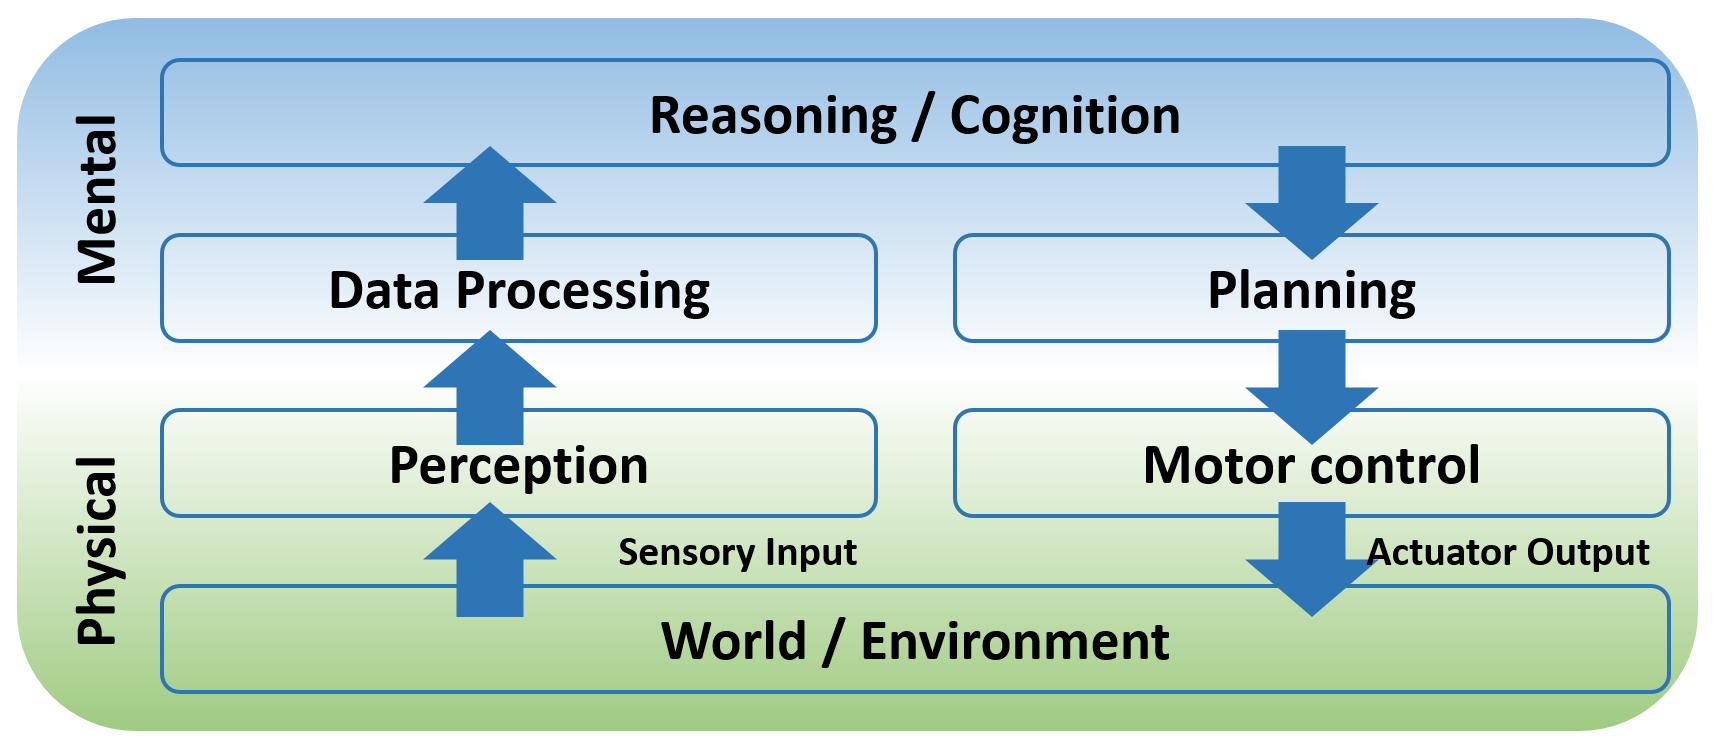
\includegraphics[width=0.85\textwidth, height=150px]{imgs/ActionPerceptionCycle.eps}
	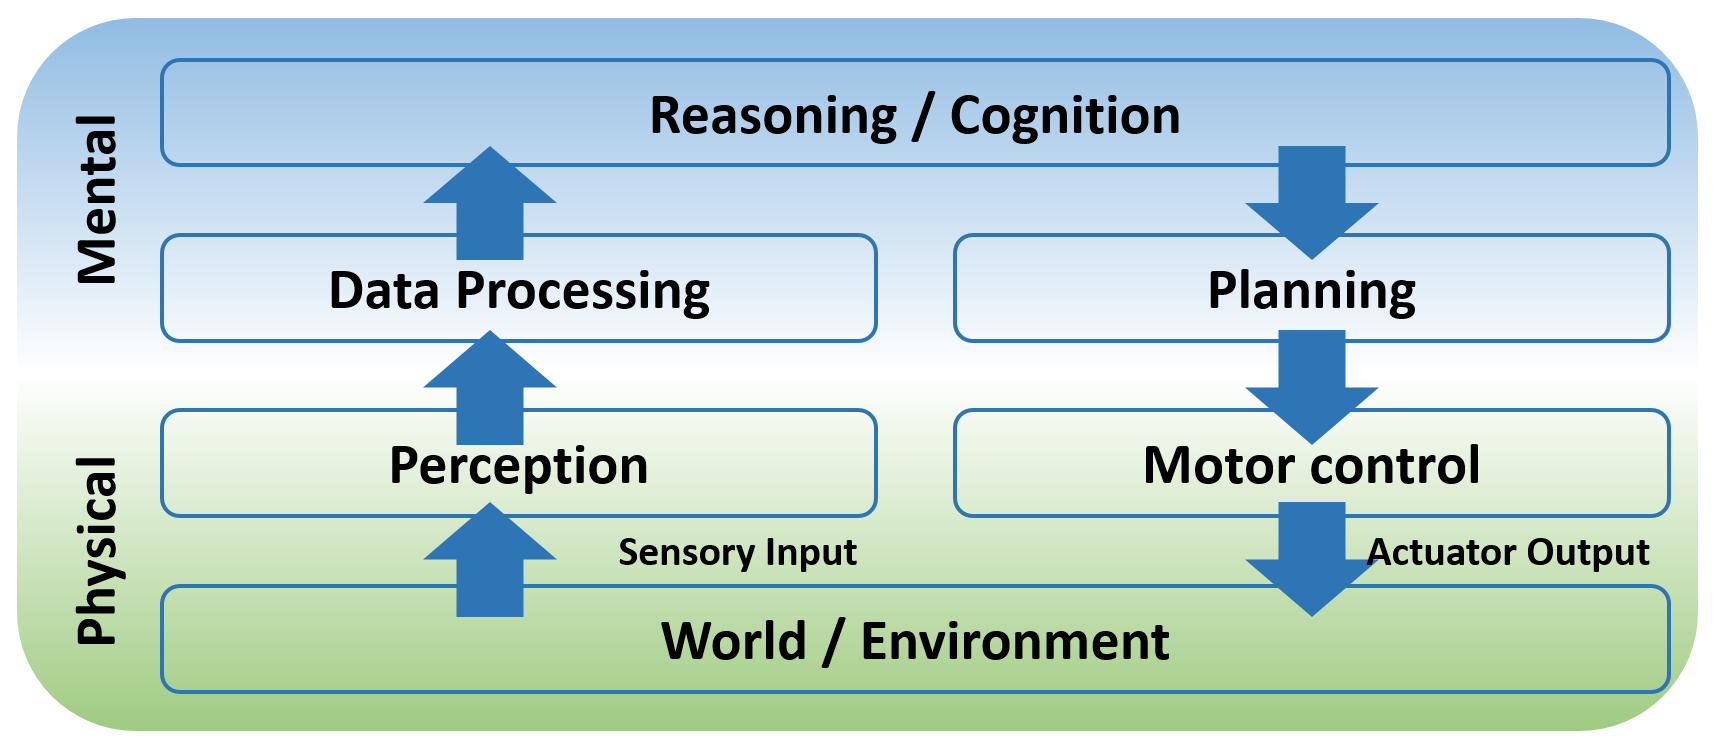
\includegraphics[width=0.85\textwidth]{imgs/ActionPerceptionCycle.eps}
	\caption{Schematic visualization of the perception-action-cycle}
	\label{fig:perc-act-cicle}
\end{figure}
Instead of considering the directional aspects of the cycle in the opposite categories of perception and action, it is also common to separate tasks in terms of hierarchy \parencite{Loeb2014}.
Interaction with the physical world through sensing and manipulation is considered on a lower hierarchical level within the perception-action-cycle while formation of mental representations and reasoning about them reside on a higher level.
We refer to those different hierarchical levels as \emph{physical} and \emph{mental} or \emph{lower} and \emph{upper} interchangeably.

Considering the physical/lower level of the perception-action-cycle, \acp{DNN} have recently shown significant progress and success at perception tasks like object detection and classification.
Therefore, we believe a lot more research is necessary until neuromorphic approaches using \acp{SNN} are sufficiently mature to compete with those traditional approaches, although current work in this directions shows promising results \parencite{Hunsberger2015}.
Similar arguments hold true for automated learning approaches regarding vehicle control.
Although sophisticated learning techniques show promise to improve motor control, to date most controllers for automated vehicles or robots in general are \enquote{designed and tuned by human engineers} \parencite{Deisenroth2013}.
One of the main reasons is the fact that control of an automated vehicle is an extremely safety-critical domain, while at the same time machine learning approaches in general pose additional challenges regarding safety validation \parencite{Koopman2016}.
Furthermore, those tasks on the physical level of the perception-action-cycle are solved effortlessly by humans and therefore, according to Moravec's paradox, we should expect them to be hard to master for artificial learning systems.
Therefore, we decided to focus on the mental/upper part of the perception-action-cycle in this thesis.
On the one hand, we believe that tasks in this part of the cycle show promise to benefit most from neuromorphic approaches.
On the other hand, \enquote{mental} tasks do not necessarily need to be performed and evaluated in closed-loop systems, which make them less problematic regarding safety issues, and therefore ideal candidates for further investigations.
It should be clear however, that \enquote{perception/action and higher level cognition are not two independent parts of one systems, but rather two integrated aspects of cognitive beings such as as ourselves} \parencite{Eliasmith2013}.
Current artificial systems are still far away from integrating both aspect effectively and more research will be necessary to close this gap.

Returning to the application domain of automated driving, precise knowledge about the current state of the environment is essential for autonomous agents and biological organisms alike to plan a secure path for navigation and to safely interact with the world.
In case of highly automated vehicles, perception of the outside world usually happens through a variety of different sensor systems such as cameras, \acs{RADAR} and \acs{LIDAR} sensors \parencite{Aeberhard2015}.
This observed information needs to be collected and combined into a central environment model, which is the (mental) basis for further reasoning and decision making.
One essential ingredient for such a model of the environment, or mental tasks in general, is knowledge or information representation.
It is an open research question to date, how the human brain represents knowledge and what underlying neural or computational substrate it uses to encode information \parencite{Wang2003, Samsonovich2012, Handjaras2016}.
Most modern approaches to reasoning or cognitive tasks in context of robotics or automated driving are built upon Bayesian probability theory and use \enquote{computer-scientific} approaches to knowledge representation.
This could be lists of objects (cf.~Fig.~\ref{subfig:urban_object_lists}) with a numerical encoding of properties when working on a higher level of abstraction.
On a lower level, another common approach especially in context of neural-network learning is to label raw sensory data, for example individual pixels of images (cf.~Fig.~\ref{subfig:urban_semantic_labels}).
However, when we as humans observe a particular scene (e.g., while driving), our mental representation will probably be very different from those aforementioned approaches.
\begin{figure}[t!]
	\centering
	\subfloat[Urban traffic scenario\label{subfig:urban_scene}]{%
		\includegraphics[width=0.45\textwidth]{imgs/urban_scene.eps}
	}
	\subfloat[Pixel-wise labels\label{subfig:urban_semantic_labels}]{%
		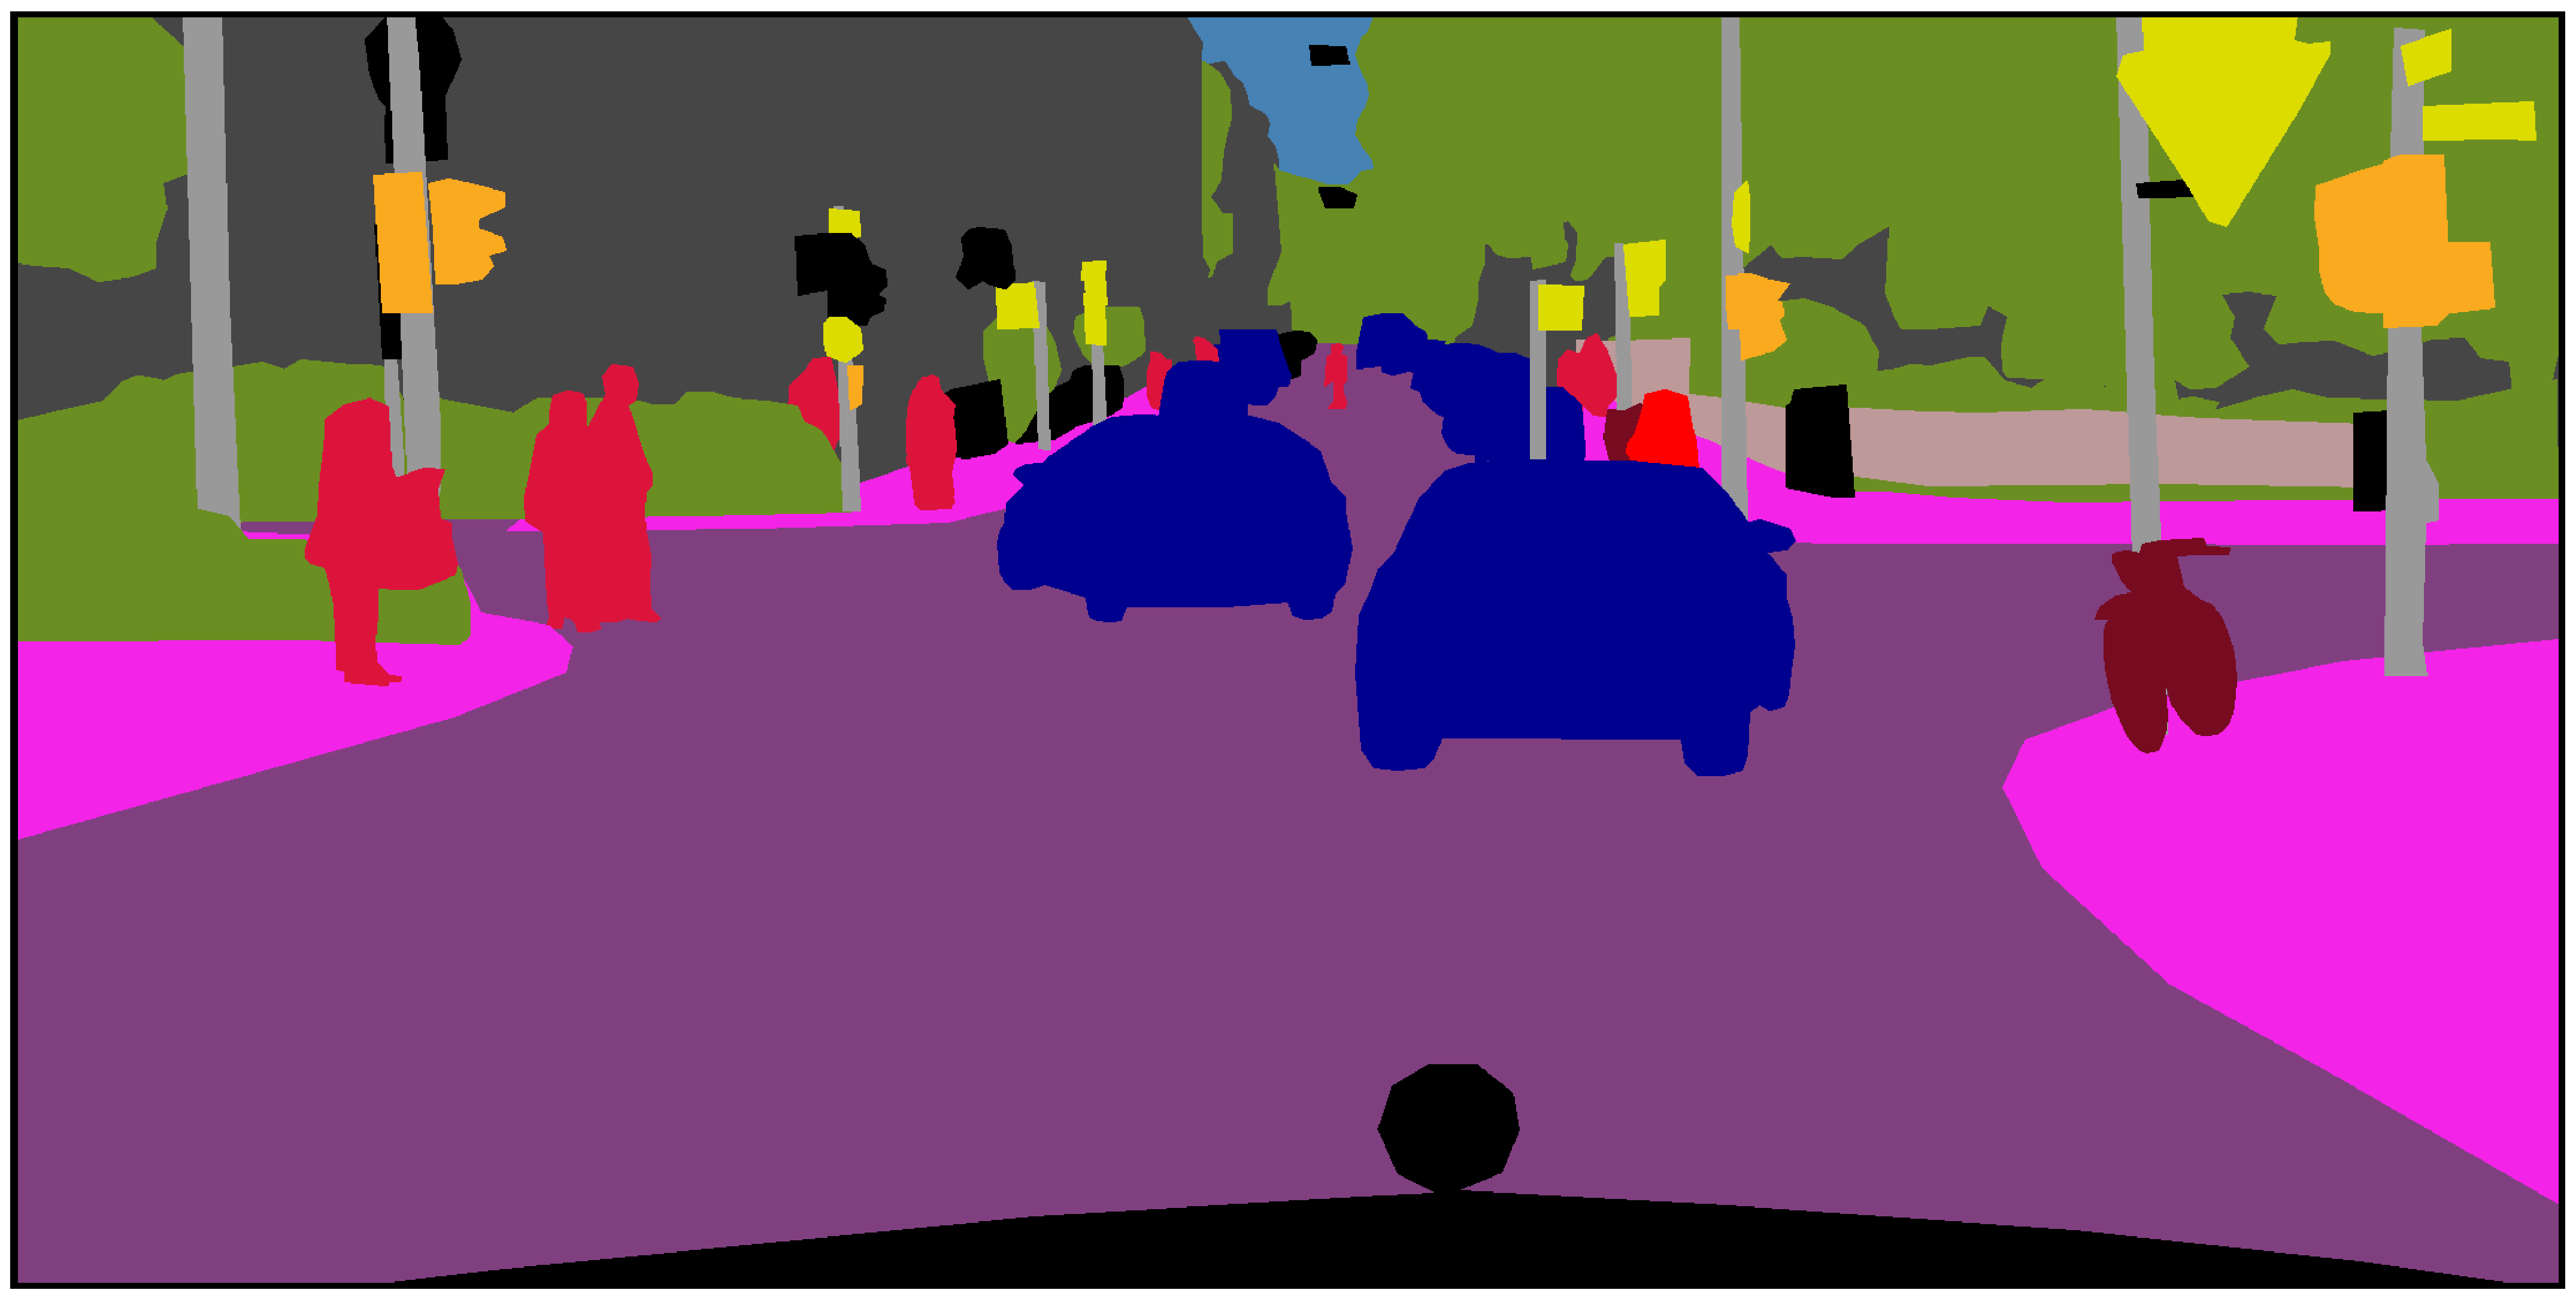
\includegraphics[width=0.45\textwidth]{imgs/urban_scene_pixel_labels.eps}
	}\\
	\subfloat[Bounding boxes indicating objects of interest\label{subfig:urban_scene_boxes}]{%
		\includegraphics[width=0.45\textwidth]{imgs/urban_scene_bound_boxes.eps}
	}
	\subfloat[Exemplary representation using lists of objects\label{subfig:urban_object_lists}]{%
		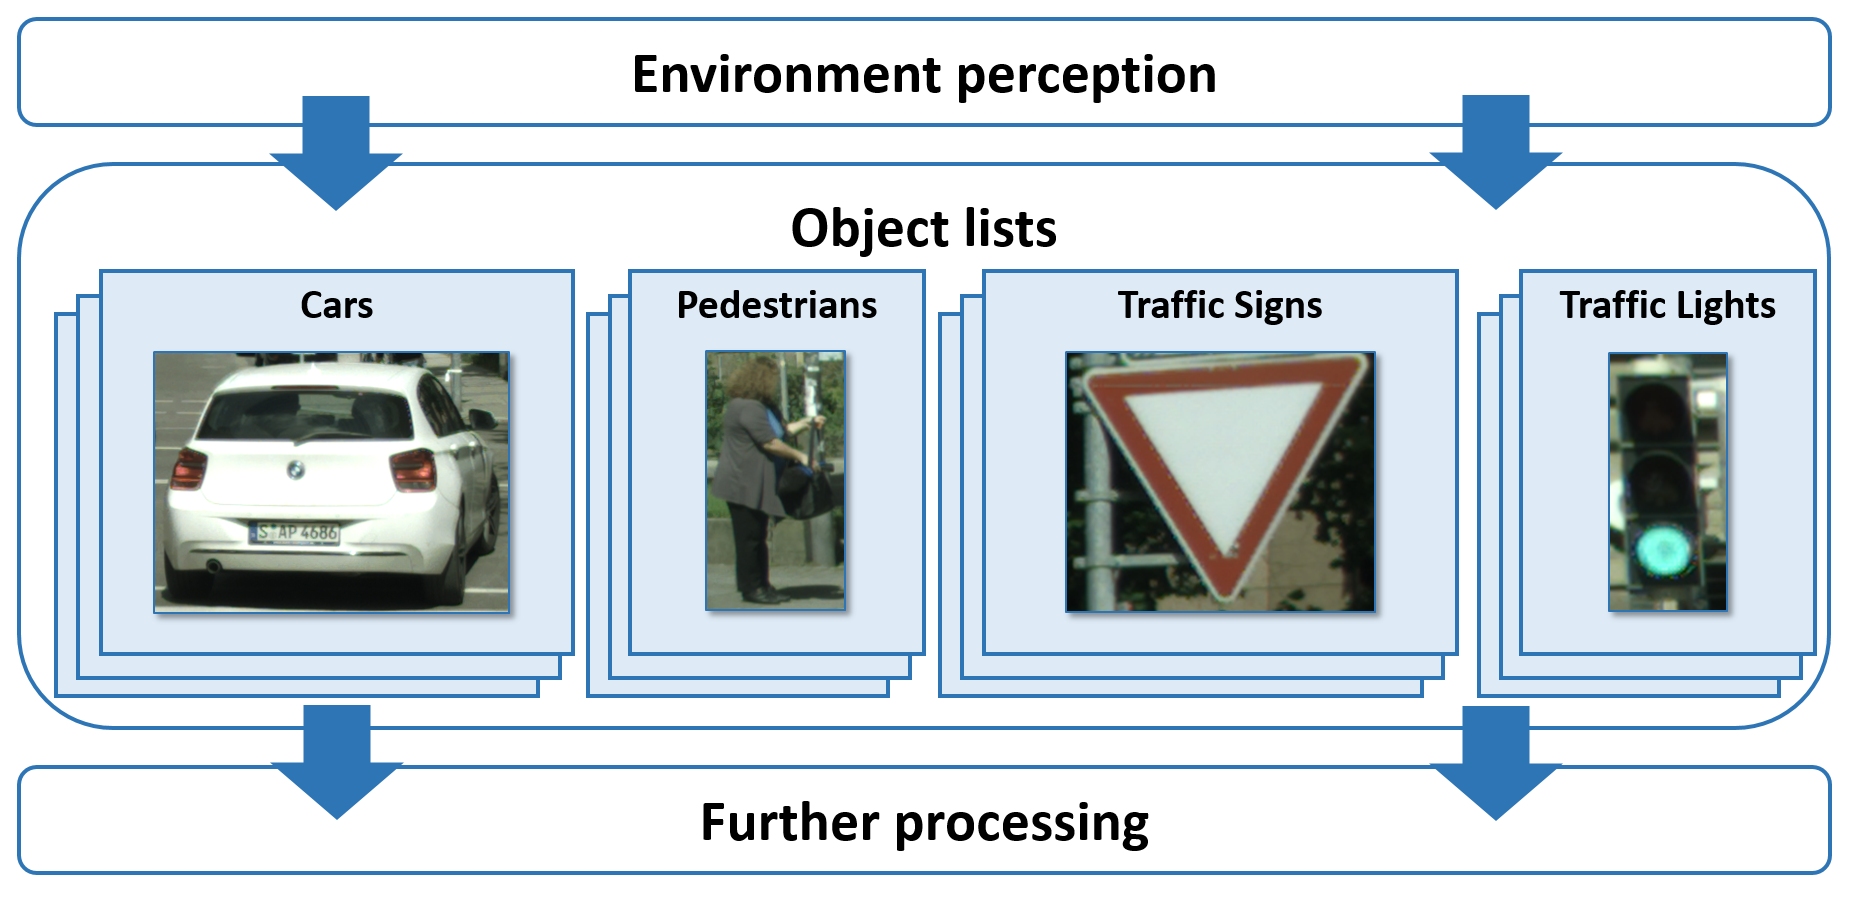
\includegraphics[width=0.45\textwidth, height=3.6cm]{imgs/urban_scene_object_lists.eps}
	}
	\caption{Example of urban driving scene with different approaches to representation. Images \ref{subfig:urban_scene}, \ref{subfig:urban_semantic_labels} and \ref{subfig:urban_scene_boxes} are (adapted) from the Cityscapes data set \parencite{Cordts2016}.}
    \label{fig:urban_scene}
\end{figure}
A human observer's representation/description of Fig.~\ref{subfig:urban_scene} would probably be in a semantic/linguistic form, for instance \emph{a blue car turning left, a white car turning right, three pedestrians waiting on the left side of the road, green traffic lights, a yield way sign}.
One common approach to encode such conceptual, semantic information or, more generally, natural language in computer-readable fashion is by using vector representations.
\acfp{VSA} is a term coined by \textcite{Gayler2003} to cover this family of modeling approaches that represent symbols or structures by mapping them to (high-dimensional) vectors.

In this thesis, we present a first step towards a cognitive environment model for automotive applications using distributed representations.
We investigate the use of these vector representations for knowledge representation and reasoning in automotive context.
This approach to information encoding is rather generic and can be applied to various different tasks with little modifications to the representation itself.
Furthermore, \acp{VSA} offer the opportunity to be implemented in a spiking neuron substrate \parencite{Eliasmith2013}, which support efficient learning algorithms and deployment on dedicated neuromorphic hardware.
This allows us to combine the advantages of symbolization with the benefits of neural networks.
We investigate varying instantiations of our representation applied to different tasks.
In a first sample application, we introduce a model learning to classify the current driving context based on a distributed representation of the current driving scene. 
The conceptual focus here is to capture semantics of the scene allowing conclusions about the type of environment the vehicle is currently navigating.
Another essential ingredient of an environment model especially in automotive context is precise knowledge about the current state and future development of all dynamic objects in the ego-vehicle's surroundings.
We focus on the task of predicting the behavior of those other traffic participants around the ego-vehicle based on a vector description of the current scene.
We hypothesize, that these structured representation have the potential to capture mutual interactions between dynamically moving agents.
Prediction of other traffic participants behavior also offers the opportunity to explore different learning approaches.
Human drivers have acquired comprehension through past experience of how other cars will probably act, but adapt this knowledge continuously when encountering new situations.
From this inspiration, we learn a generic model of dynamic behavior through offline (i.e., batch) training and refine this model when perceiving behavior of a particular object through online learning.
To complement the more high-level reasoning tasks with a perspective on motor control, we also introduce a novel neuromorphic control architectures, that can be used to implement generic control algorithms in the language of \acp{SNN}.
This approach allows to divide larger tasks in small sub-networks combining the advantages of manual programming with neural network learning.

\section{Outline of the thesis}%
\label{sec:outline_of_the_thesis}

This section provides a brief overview of the thesis structure as well as a short summary for each chapter.
Chapter~\ref{chap:research_context} summarizes the state-of-the-art in several areas related to the core of the thesis at hand spanning from biologically inspired hardware and software over cognitive modeling techniques to automated driving research.
We give an overview over all of these sub-topics providing a detailed description where necessary while putting these details in context of a bigger picture.

Chapter~\ref{chap:introduction_to_vsas} introduces the key ingredients for the models developed in later chapter, distributed representations and \acp{SNN}, and establishes the mathematical apparatus and the essential theoretical properties of these ingredients.
After proposing a more rigorous mathematical formalism to describe the general theory of \acp{VSA}, we proceed to the \ac{SPA} as a special case of \acp{VSA} with additional features and theory to be presented.
Furthermore, we give an introduction to the general ideas for cognitive modeling based on \acp{VSA} like vocabularies and structured representation generation.
Furthermore, we present a brief description of the \ac{NEF} and how it can be used to implement cognitive architectures based on vector representations in a spiking neuron substrate.

In chapter~\ref{chap:a_cognitive_approach_to_represent_automotive_scenes}, we proceed to present the general approach to encode automotive scenes in semantic vectors as representational substrate.
We show different approaches to generate vector vocabularies, which are the basic ingredients to built more complex, structured representations from them.
We demonstrate successful embedding of several similarity structures into vector vocabularies designed for automotive applications.
Additionally, we present several approaches to representing numerical values in our vector substrate introducing a novel approach based on a convolutive power, generalizing exponentiation to circular convolution.
We conclude the chapter with a thorough analysis regarding the systematic limitations regarding the vectors capacity, i.e., amount of information such vector representations can effectively store.

Chapter~\ref{chap:driving_context_classification} introduces the first sample instantiation of our vector representation applied to the task of driving context classification based on a scene vector encapsulating the current driving situation.
We establish the vector-based scene representation for the context classification task and use it as input data to a learning model implemented in a spiking neuron substrate.
To evaluate the model's performance, we present several reference learning systems using either the vector representation or visual information as input and compare them to human level performance.
Finally, we analyze the influence of the underlying vocabularies encoding different similarity structures on the learning model's classification performance.
All evaluations are conducted using real-world driving data.

In chapter~\ref{chap:behav_pred}, we introduce a second instantiation of our scene representation to predict the behavior of other objects in the vehicle's surroundings.
In the context of vehicle trajectory prediction, we employ our novel approach to encode spatial information in distributed representations to encode the positions of several vehicles in vectors of fixed length.
We employ neural networks built from \ac{LSTM} units as well as simpler single-layer \acp{SNN} to predict vehicle trajectories based on past motion.
We analyze the influence of hyperparameters, information provided to the models as well as the composition of the training data on the models' prediction accuracy.
Furthermore, we compare the models with respect to situations in which one particular model outperforms the others.
Finally, we show that it is generally possible to detect abnormal samples indicating potentially dangerous situation based solely on the distributed vector representation and unsupervised learning.
The evaluation conducted in the chapter uses data from two different data sets containing real-world driving data.

Chapter~\ref{chap:mix_online_learning} introduces an extension of the proposed trajectory prediction models for online adaptation through incremental learning.
Building on the findings in chapter~\ref{chap:behav_pred}, we present a novel mixture-of-experts model implemented in a spiking neuron substrate meant to be trained at run time to improve the prediction performance over several individual predictors.
One of the strengths of this model is that, instead of having to start from a completely blank state, it relies on several expert models, which have been previously trained and validated offline.
This model, like all models making predictions about the future, faces the issue that the actual motion of the predicted vehicle needed to compare the model's anticipated values to is future data and thus not available at the time the model actually makes its predictions.
To avoid potentially long delays in the online learning process, we propose a novel approach to spread the error signal of earlier predictions over later predictions.
Revisiting the data sets used in chapter~\ref{chap:behav_pred}, we evaluate two different variants of the mixture models adapting their weights either solely based on the prediction error or the current context of the scene.
We show, that our online learning model is able to improve over the individual predictors already after being exposed to a small set of example vehicles.

Chapter~\ref{chap:closed_loop_neuromorphic_control_systems} presents a first step towards a neuromorphic control architecture by developing two sample instantiations of neurally-inspired control algorithms.
We establish neuromorphic control architectures, that can be used to implement generic control algorithms in the language of \acp{SNN} with the advantage, that the overall task can be divided into several sub-networks.
This approach allows us to combine manual programming with the advantages of neural network learning.
Manually programmed sub-tasks can either complement learning networks within the system or serve as an initial approximation of the desired function, which allows more directed learning to improve task performance avoiding the need to start learning from a completely blank state.
As mentioned earlier, control of an automated vehicle is an extremely safety-critical application.
Hence, we present two sample applications in simplified setups: one on mobile robot manipulation demonstrating initial manual programming of a non-trivial robotic task in a spiking neuron substrate and one on vehicle trajectory control demonstrating how manually programmed modules can be complemented by learning networks.

Chapter~\ref{chap:discussion} summarizes the work and interprets the results achieved in this thesis.
We discuss the main advantages of the representations and models proposed in this work while also addressing limitations indicated by either systematic or experimental analysis.
We conclude the thesis by proposing a series of extensions and improvements, which potentially contribute to adopting the principles investigated in this thesis on a wider scale to obtain a more mature representation framework for automotive applications.

\section{Contributions of and to this thesis}%
\label{sec:contributions_of_and_to_this_thesis}

This thesis presents a first step towards a cognitive environment model for automated vehicles and thereby a provides a novel perspective to knowledge representation in automotive context.
The two key ingredients for our approach are distributed representations and \acp{SNN}, which in combination offer a promising modeling substrate for cognitive tasks as shown in \textcite{Eliasmith2013, Eliasmith2012}. 
The possibility to implement distributed representations in a spiking neuron substrate offers the potential to combine symbol-like processing with the strength of neural network learning.
Additionally, \acp{SNN} are one option to tackle increasing energy-efficiency requirements in future automated vehicles equipped with a plethora of sensors and computing systems.
This thesis presents a strict mathematical formalism regarding the theory of distributed representations, summarizing their key features in a generic framework.
Thereby, we lay the foundation for our novel approach to build structured representations of automotive scenes.
We demonstrate the general feasibility of our approach in two sample instantiations.
For all the models and representation approaches investigated in this thesis, we present a thorough and detailed analysis regarding parameters and accuracy including a comparison to several baseline models.
While the models employing our structured representations achieve promising results in terms of accuracy without clearly outperforming more traditional approaches, we expect the critical benefits of our approach to be revealed when being actually deployed on specialized computing hardware. 
As shown by \textcite{Hunsberger2016}, implementing learning models in \acp{SNN} is often a trade-off between energy-efficiency and accuracy.
Finally, we establish neuromorphic control architectures, that can be used to implement generic control algorithms in the language of \acp{SNN}.
This approach can benefit from splitting larger tasks in small sub-networks, that can be manually programmed to complement or bootstrap learning networks.

This dissertation was supported by the \ac{BMW} AG, where I was employed as doctoral candidate and later in a permanent position during the preparation of this thesis.
Therefore, parts of the literature review and text that presents the research context in chapter~\ref{chap:research_context}, especially the section on neuromorphic computing hardware, was conducted in collaboration with \ac{BMW} colleagues.
The research on the mobile manipulation task was conducted during a collaboration project between \ac{TUM} and University of Waterloo while the work on vehicle trajectory control was supported by Benjamin Zorn during his internship at \ac{BMW}.
The approaches, principles and models presented in the sections on structured vocabularies in chapters~\ref{chap:a_cognitive_approach_to_represent_automotive_scenes} and~\ref{chap:driving_context_classification} were developed in collaboration with Robert Darius during the preparation of his Master's thesis \parencite{Darius2018} under my supervision at \ac{BMW} Group.
Many of the novel approaches presented in this thesis arose from discussions with researchers from the \ac{CNRG} at University of Waterloo, where I spent a six week research visit in summer 2017.
This research visit spawned a follow-up collaboration project between \ac{BMW} and \acf{ABR}, during which parts of chapters~\ref{chap:behav_pred} and~\ref{chap:mix_online_learning} were developed in collaboration.
This collaboration covered mainly the implementation of the \ac{LSTM} model based on numerical input in chapter~\ref{chap:behav_pred} as well as discussions about the online learning approach presented in chapter~\ref{chap:mix_online_learning}.
Researchers involved in this collaboration co-authored some of the publications listed in~\ref{subsec:list_of_publications}.
Finally, figures displayed in this thesis, which have been reprinted or adapted from others or quotations are clearly marked as such.
Anything not indicated as quotation or external source is the author's original work.

\subsection{List of Publications}%
\label{subsec:list_of_publications}

The following list gives an overview of the publications written and submitted during the preparation and work on this thesis.
Beside published articles, we also list submitted or already accepted manuscripts waiting for final publications at the time of submission of this thesis.

\subsubsection{Published peer-reviewed journal papers}
\begin{enumerate}
	\item \printpublication{Mirus2018a}
\end{enumerate}

\subsubsection{Published peer-reviewed conference papers}
\begin{enumerate}
    \item \printpublication{Mirus2019c}
	\item \printpublication{Mirus2019}
	\item \printpublication{Mirus2019a}
	\item \printpublication{Mirus2018}
\end{enumerate}

\subsubsection{Submitted peer-reviewed journal papers}
\begin{enumerate}
	\item \printpublication{Mirus2019b}
\end{enumerate}


\chapter{Research Context}
Highly automated driving is currently an immensely attractive field for both academic and industrial research groups. 
A fully autonomous vehicle, which is able to tackle challenging driving situations without external input comparable to a human driver's performance, is yet to be build.
In this thesis, we propose a novel approach to knowledge and information representation for automotive environment models using cognitive modelling techniques.
More precisely, we adopt \acfp{VSA}, which are commonly used in tasks like cognitive modelling and natural language processing, for the specific application of automotive environment modelling.
To our knowledge, \acp{VSA} have not been applied in this particular context. 
In order to put our work in context of the current research landscape and to circumscribe this thesis, we need to review related work from several different areas like automated driving and mobile robotics, computational neuroscience, artificial intelligence and neuromorphic engineering.
A comprehensive overview for all of these research areas is out of scope of a single thesis.
However, we aim to cover the most significant results from all areas at least briefly, whereas we present an in-depth review of relevant work related to the thesis at hand, where necessary.

\section{Automated Driving}
"Robotics is the science of building computer-controlled mechanical devises, which are able to perceive and manipulate the physical world" \cite{Thrun2005}.
Automated driving in automotive context is a special case of robotics, since an autonomous vehicle can be considered a wheeled mobile robot, which is able to fulfill the transportation capabilities of a traditional car without human input. 
In order to navigate safely to a desired goal, a mobile robot needs to solve several problems like localization ("where am I?"), path planning ("how do I get from A to B?"), environment perception ("where is everyone else?"), knowledge representation and reasoning ("which decisions to infer from available information?") as well as motion control ("how to move my actuators?").
In automotive context, an automated vehicle furthermore needs to detect the current state of the driver ("what is the driver up to") to ensure that he can take over control in safety-critical situations or in case of malfunctions.
The human driver as a fallback option in such situations is of crucial importance, since the level of driving automation gradually increases instead of a hard transition to automated driving systems.
In their J3016 standard \cite{SAE_J3016}, the \ac{SAE} delivers a classification system identifying six different levels of driving automation from "no automation" to "full automation".
Table \ref{tab:autonomy_levels} gives an overview of the particular automation levels according to \cite{SAE_J3016} in more detail.\\
On the road to fully automated driving, several \ac{ADAS} have been developed during the last decades and thus made a huge jump by incrementally increasing complexity and therefor the level of autonomy.
The history of automated driving research goes back to the 1980's, when governmental institutions funded several explorative projects worldwide to research functionalities like automatic vehicle driving and intelligent route planning resulting in early prototypes.
In 1986, several European research groups and vehicle manufacturers started the \ac{PROMETHEUS} project \cite{Dickmanns1990} and demonstrated a variety of different approaches to automated driving.
Another research initiative established during that period is Carnegie Mellon University's Navlab \cite{Thorpe1988}, which achieved the first completely autonomous drive from Pittsburg to San Diego.
After that first explorative phase, the US government established the \ac{NAHSC} in 1995 and shortly shortly followed by the foundation of the \ac{AHSRA} 1996 in Japan.
The main contribution of this first phase was the identification and deep analysis of problems, that would need to be tackled by researchers, to understand requirements and possible effects of future automated vehicles.
\cite{Bertozzi2000} gives an overview of the achievements and perspectives obtained in the projects during that period.\\
\begin{center}
	\begin{tabular}{|c | l | p{10cm}|}
		\hline
		\textbf{Level} & \textbf{Name} & \textbf{Narrative Definition}\\ \hline
		0 & No Automation & the full-time performance by the human driver of all aspects of the dynamic driving task, even when enhanced by warning or intervention systems \\ \hline
		1 & Driver Assistance & the driving mode-specific execution by a driver assistance system of either steering or acceleration/deceleration using information about the driving environment and with the expectation that the human driver perform all remaining aspects of the dynamic driving task \\ \hline
		2 & Partial Automation & the driving mode-specific execution by one or more driver assistance systems of both steering and acceleration/deceleration using information	 about the driving environment and with the expectation that the human driver perform all remaining aspects of the dynamic driving task \\ \hline
		3 & Conditional Automation &  the driving mode-specific performance by an automated driving system of all aspects of the dynamic driving task with the expectation that the human driver will respond appropriately to a request to intervene \\ \hline
		4 & High Automation & the driving mode-specific performance by an automated driving system of all aspects of the dynamic driving task, even if a human driver does not respond appropriately to a request to intervene \\ \hline
		5 & Full Automation & the full-time performance by an automated driving system of all aspects of the dynamic driving task under all roadway and environmental conditions that can be managed by a human driver \\ \hline
	\end{tabular}
	\label{tab:autonomy_levels}
	\captionof{table}{Table depicting different levels of vehicle automation identified in \cite{SAE_J3016}}
\end{center}
A major milestone in the research field of automated driving was the first \ac{DARPA} Grand Challenge in 2004, where unmanned vehicles had to complete a \SI{240}{\kilo\meter}, unrehearsed off-road course autonomously through the Mojave Desert in Nevada to win the price money of \$1 million. 
Although no participating vehicle successfully finished the race \cite{Bacha2004} in the first challenge, valuable insights have been gained.
Using those insights to make significant progress, five teams (out of 23) were able to successfully complete the second \ac{DARPA} Grand Challenge in 2005 with Stanford's Stanley robot winning first place \cite{Thrun2006}.
After the success of the second Grand Challenge, the \ac{DARPA} organized the Urban Challenge in 2007, switching the focus to automated driving in urban environments \cite{Buehler2009}.
In this competition, vehicles had to complete a \SI{97}{\kilo\meter} urban area course autonomously in less than \SI{6}{\hour}, while obeying California state driving laws, avoiding other participating vehicles and other objects using only on-board sensors and \ac{GPS}.
Six vehicles out of the 11 final participants successfully finished the competition, with Carnegie Mellon's Boss robot \cite{Urmson.2008} being named the winner finishing the course in little over \SI{4}{\hour} with an average speed of approximately \SI[per-mode=symbol]{22.5}{\kilo\meter\per\hour}.
\\
The technology developed for the \ac{DARPA} challenges formed the basis for commercial \ac{ADAS}, which have seen rapid progress since then and gradually made their way into series-production vehicles.
There exists a large variety of commercial systems, like e.g. \ac{ACC} or intelligent parking assistance systems, modern vehicles are already equipped with.
These systems have the potential to increase comfort and safety in road traffic and, in the long run enable fully autonomous driving (cf. Level 5 in Table \ref{tab:autonomy_levels}). 
On the other hand, many research teams and initiative were spawned or inspired from \ac{DARPA} Challenges these competitions and continued their research work after the .
\begin{figure}[t!]
	\centering
	\resizebox{.9\textwidth}{!}{%
	\subfloat[\label{subfig:stanley}]{%
		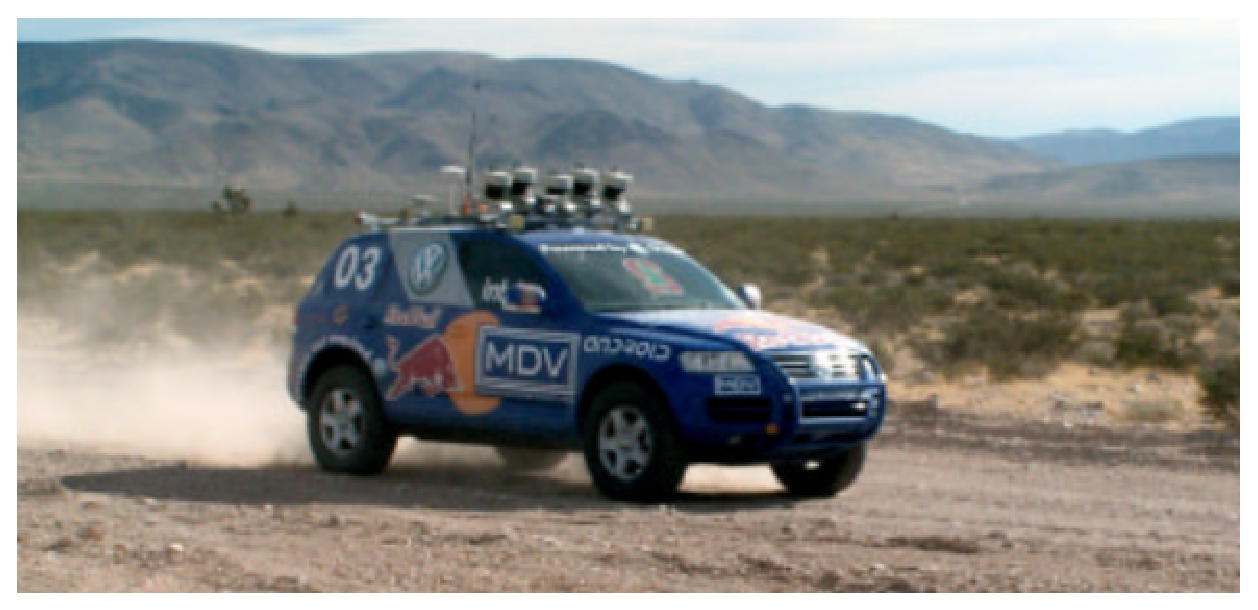
\includegraphics[height=3cm]{imgs/Stanley.eps}
	}
	\subfloat[\label{subfig:boss}]{%
		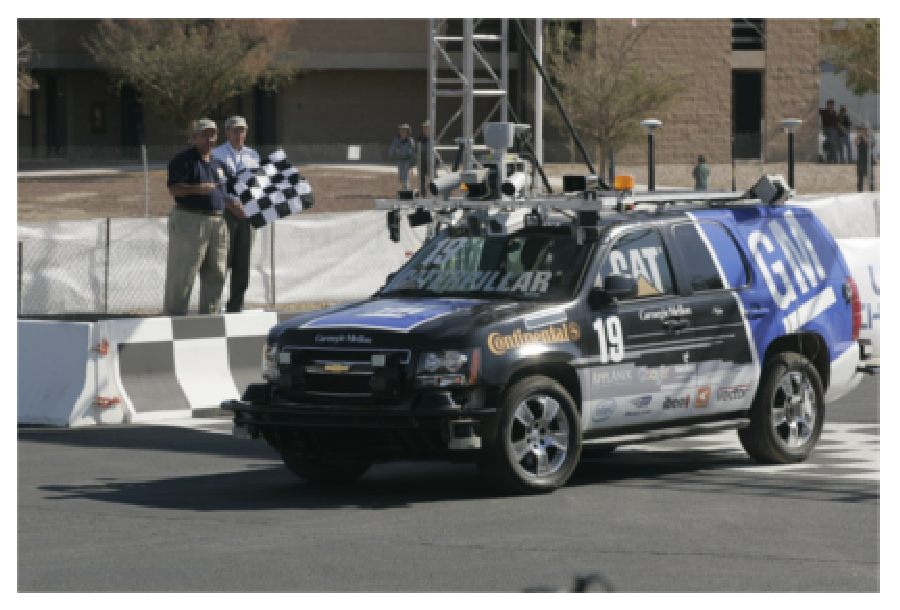
\includegraphics[height=3cm]{imgs/Boss_DARPA_urban_challenge.eps}
	}
}
	\caption{The winning robots from the 2005 \ac{DARPA} Grand Challenge and 2007 Urban Challenge. Fig. \ref{subfig:stanley} shows Stanford's Stanley at the 2005 \ac{DARPA} Grand Challenge (Image from \cite{Thrun2006}), Fig. \ref{subfig:boss} shows Carnegie Mellon's BOSS at the 2007 \ac{DARPA} Urban Challenge (Image from \cite{Urmson.2008}).}\label{fig:darpa_chal}
\end{figure}
Many researchers involved in the winning teams continued their research within Google's self-driving car project, which started in 2009 and evolved into the Spin-Off company Waymo \cite{Waymo} in 2016.
Another research team continuing their efforts after the \ac{DARPA} challenges is the Annieway team \cite{Annieway}.
One of their major contributions is the release and maintenance of the KITTI vision benchmark suite \cite{Geiger2013IJRR}, a publicly available data set containing data from various test drives in the city of Karlsruhe, rural areas as well as highways focusing on providing real world data for vision tasks like stereo, optical flow and 3D object detection and tracking.\\
The main research goal after the \ac{DARPA} Challenges was to develop automated driving with off-the-shelf sensors \cite{Furgale2013}.
As this thesis focuses on environmental modelling in context of autonomous driving, this section presents research from this field like road detection and modelling (Sec. \ref{subsec:lane}), object detection (Sec. \ref{subsec:obj_detect}) and tracking (Sec. \ref{subsec:obj_track}) as well as sensor fusion (Sec. \ref{subsec:sensor_fusion}) while other aspects like localization \cite{Levinson2010, Thrun2005}, path planning (\todo{citation}) and motion control (\todo{citation}) are neglected.
\subsection{Object Detection and Classification}
\label{subsec:obj_detect}
\subsection{Behaviour Analysis}
\label{subsec:behav_analysis}
\section{Neuromorphic Systems}
To fully understand biological systems like the brain, which evolved over millions of years, is an ongoing yet unsolved challenge in biology and neuroscience.
Even small animals like insects or rodents show remarkable behavioural flexibility and the ability to constantly adapt to a rapidly changing and noisy world, which is unmatched by modern computing machines.
Mammals and primates are able to perform more sophisticated behaviours culminating in complex cognitive computations humans are capable of doing like thinking, problem solving, memory, reasoning, decision making, strategic planning, knowledge representation, learning etc.
The "biological computer" enabling these behaviours and cognitive abilities is the brain consisting of large networks of neural cells (or neurons), which communicate by sending and receiving electric signals via synapses.
At the same time, brains are comparably small and efficient: the human brain for example consumes only \SI{20}{\watt} of power (equivalent to a compact fluorescent light bulb) and comprises \SI{2}{\percent} of the body weight \cite[Chap. 2.1]{Eliasmith2013}. \\
Several research fields like computational neuroscience, neuromorphic engineering and neurorobotics try to reverse engineer biological systems to achieve similar performance and computational power.
During the last decades, researchers and engineers strived to close the gap in performance and efficiency between biological and artificial computing systems by mimicing neuro-biological architectures in hardware and implementing models of neural systems in software.
This biologically inspired, \textit{neuromorphic} approach promises not only to perform computations in a more efficient way, but also to tackle problems unsolvable with current computing machines.
\subsection{Historical remarks}
\begin{figure*}[t!]
	\centering
	\includegraphics[width=0.95\textwidth,height=270px, natwidth=944,natheight=350]{imgs/Neuromorphic_Timeline_alpha.png}
	\caption{Historical developments in computational neuroscience, neuromorphic engineering and machine learning.\todo{check and possibly update this figure}}
	\label{fig:neuro_time}
\end{figure*}

The term neuromorphic itself was first introduced by Carver Mead in the late 1980s \cite{Mead90}, when describing one of the first silicon retinas.
He called artificial systems that share organization principles with biological nervous systems neuromorphic.
An interesting prototype of a silicon retina, which is now considered a milestone, was implemented by Misha Mahowald, a PhD student of Carver Mead. 
Her thesis received Caltech's Milton and Francis Clauser Doctoral Prize for its originality and potential for opening up new avenues of human thought and endeavor.
Since these early days of neuromorphic engineering, the term has widely been used to describe \ac{VLSI} systems \cite{Mead1989}, novel computing devices \cite{Schemmel2010}, sensory systems \cite{Lichtsteiner2008, Liu2010}, software \cite{Davison2008, Bekolay2014} and algorithms \cite{ReverterValeiras2016}.
Considering the number of scientists, neuromorphic engineering is still a comparably young field of research but received an increased interest during the last decade from both academic and industrial research groups caused by the funding of large, ambitious projects.
Although there have been several achievements in the field during the 1990s \cite{Mead1989, Mahowald1992, Indiveri1997, Cauwenberghs1998} and early 2000s \cite{Liu2002}, the \ac{FACETS} project \cite{FACETS-proj} and the \ac{BBP} \cite{BlueBrain-proj}, both starting in 2005 and mainly funded by the \ac{EU} under the FP6-\ac{FET} program, were among the first big-budget neuromorphic projects.
The follow-up project \ac{BrainScaleS} \cite{BrainScaleS-proj, Schemmel2010} (2011-2015) built on and extended the research conducted during the \ac{FACETS} project. 
The main developments of the \ac{FACETS} and \ac{BrainScaleS} projects are the \ac{HICANN} chip \cite{Schemmel2010} and the Python-based simulator-independant language \ac{PyNN} \cite{Davison2008} for building neural network models.
Building on \ac{BBP} the \ac{BrainScaleS} hardware development is currently continued in the neuromorphic computing platform of \ac{HBP} \cite{HBP-proj, Calimera2013}, a large ten-year research project, which was selected as one of the two \ac{EU}-\ac{FET} flagships in 2013 and is granted around one billion euros funding.
Another project starting in 2005, initially funded by the UK government until 2014 and now also part of the neuromorphic computing platform of \ac{HBP}, is the \ac{SpiNNaker} project \cite{Furber2014} during which the neuromorphic computing hardware of the same name was developed.
The \ac{HBP} is organized in thirteen platforms in total, which focus on different research fields related to the brain like for example theoretical neuroscience, neurorobotics, cognitive architectures, high performance computing, brain simulation and the aforementioned neuromorphic computing platform (see \cite{HBP-proj} for details).\\
Beside these research activities in Europe, the \ac{DARPA} funded another big-budget neuromorphic project: the \ac{SyNAPSE} program \cite{SYNAPSE-proj, Srinivasa2012}, which started in 2008 and is scheduled to run until 2016, has received 102.6 million US dollars in funding as of January 2013. 
The program aims to build an electronic microprocessor system that matches a mammalian brain in function, size, and power consumption.
Achievements during the \ac{SyNAPSE} program, which is primarily contracted to IBM Research and \acs{HRL}, so far are include brain simulations, design of brain-inspired neuromorphic achitectures \cite{Nere2012} and the development of a digital neurosynaptic core \cite{Merolla2011}, which is a building block of IBM's recently published TrueNorth chip \cite{Akopyan2015}.
Further project results are the Corelet language \cite{Amir2013} and the simulator Compass \cite{Preissl2012}, which enable dedicated software development as well as simulation and testing of TrueNorth algorithms on standard hardware respectively.\\
Beside these projects, the neuromorphic community is coming together at two annual (three- resp. two-week) workshops in Telluride and CapoCaccia, which have been established in 1994 and 2007 respectively, to discuss the current state of research in lectures and interactive talk sessions, to forge new ideas and to work on hands-on projects in small workgroups.\\
The original definition of neuromorphic engineering also covers \acp{ANN} in general.
This research field even goes back to the 1940s when McCulloch and Pitts introduced artificial neurons as computational units \cite{McCulloch1988}, which embody a simplified model of biological neurons.
These first simple networks were able to calculate compositions of basic logic functions \cite{McCulloch1988, Rojas1996}.
Rosenblatt \cite{Rosenblatt58} proposed the first neural network, which was capable of learning, by adding numerical weights to the connections of the network with threshold functions as activation functions: the \textit{perceptron}.
Minsky and Papert \cite{Minsky1969} showed, that single-layer perceptrons are not able to calculate an XOR-function or, more generally, are only capable of learning linearly separable patterns.
This caused a decreased interest in neural networks research until the rediscovery of the backpropagation algorithm \cite{Werbos1974} in the 1980s \cite{Rumelhart1988}, which introduced a practically feasible method to optimize the network weights using gradient descent and led to a resurgence of neural network research.
%This gradient descent called for continuous activation functions (mostly sigmoid or hyperbolic) instead of threshold-functions as activation functions, which made the so-called second generation \ac{ANN} universal approximators for continuous functions \cite{Cybenko1989}.
Since then, various different network architectures like feed-forward, \acp{CNN}, \acp{RNN}, \acp{RBF}, \acp{RBM}, \acp{SOM} and \ac{ART} just to name a few \cite{Schmidhuber2015} have been proposed for different learning paradigms.
Although several simpler methods like Boosting \cite{Freund1997} or \acp{SVM} \cite{Vapnik1995} have been developed and achieved noteworthy results, the availability of powerful, parallelized computing hardware like \acp{GPU} as well as the advent and success  of deep learning (partly achieving better-than-human accuracy) made \acp{ANN} \cite{Rojas1996} and especially \acp{DNN} \cite{LeCun2015} the state-of-the-art for several machine learning tasks like visual digit \cite{Ciresan2012a} and traffic sign \cite{Ciresan2012} recognition in recent years.
Another great achievement in the field of deep learning was the victory of AlphaGo \cite{Silver2016} over the world's best Go player Lee Sedol in March 2016, which was considered to be at least a decade away due to the complexity of Go.
Compared to Deep Blue, the system that beat former chess world champion Garri Kasparov in 1997 \cite{Hsu2002} with sheer computational power by brute forcing through a large number of possible moves in advance to find the best one, this strategy is not feasible for Go due to its higher complexity (larger board, more options to consider per move).
In contrast, modern \acp{DNN} trained by a combination of supervised learning from human expert games and reinforcement learning from self-play have been used for the evaluation of board positions and selection of moves to avoid expensive lookahead search \cite{Silver2016}.
A comprehensive and historical overview of relevant literature concerning \acp{ANN} and especially \acp{DNN} can be found in \cite{Schmidhuber2015, LeCun2015}.

%----------------------------------------------------------------------------------------------------------
\subsection{\aclp{ANN}}
\label{subsec:ML_ANN}
%----------------------------------------------------------------------------------------------------------
Machine learning is the science of constructing computer programs, which improve with experience. 
This is attractive if manually programming a desired functionality is not cost-efficient, intractable or simply impossible.  
The overall goal of machine learning algorithms is to generalize beyond examples, i.e. to generate models that describe the presented input sufficiently well to make the best possible prediction when confronted with previously unseen data.
A formal, widely cited definition of machine learning has been presented by Thomas M. Mitchell in \cite{Mitchell1997}:

\begin{defn}
	A computer program is said to \textbf{learn} from experience $E$ with respect to some class of tasks $T$ and performance measure $P$ if its performance at tasks in $T$, as measured by $P$, improves with experience $E$.
\end{defn}
A large body of research has focused on machine learning during the last decades.
From the first theoretical considerations concerning artificial neural networks by McCulloc and Pitts(\todo{Citation}) in the 1940s and the first Multilayer-Perceptrons by Rosenblatt (\todo{Citation}) about a decade later, machine learning algorithms started to receive widespread attention with the rediscovery \cite{Rumelhart1988} of the well-known backpropagation algorithm \cite{Werbos1974}.
Since then, several approaches to machine learning, apart from artificial neural networks, like AdaBoost (\todo{Citation}), Decision Trees (\todo{citation}), Bayesian Networks (\todo{citation}) or \ac{SVM} (\todo{citation Vapnik, V. (1995), The Nature of Statistical Learning Theory. Springer Verlag, Cristianini, N. and Shawe-Taylor, J. (2000). An Introduction to Support Vector Machines and Other Kernel-Based Learning Methods. Cambridge University Press, Cambridge}) have been proposed.
These methods vary in representation of the data, the evaluation (or objective) function, the optimization technique and the learning paradigm.
Through availability of larger datasets and increased computational power, machine learning has seen significant progress in recent years.
The use of deep neural networks \cite{Schmidhuber2015}, enabled through modern, powerful computing hardware like \ac{GPU}, yielded a significant performance boost in several classification tasks. 
Today, modern deep learning algorithms can even rival human performance on different visual classification tasks like traffic sign \cite{Ciresan2012} or digit recognition \cite{Ciresan2012a}.

So-called second generation \ac{ANN} introduced continuous (e.g. sigmoid or hyperbolic) instead of step- or threshold-functions (\todo{Citation}) as activation functions, which made them universal approximators for continuous functions \cite{Cybenko1989}.

%----------------------------------------------------------------------------------------------------------
\subsection{\aclp{SNN}}
\label{subsec:SNN}
%----------------------------------------------------------------------------------------------------------
\begin{figure}
	\centering
	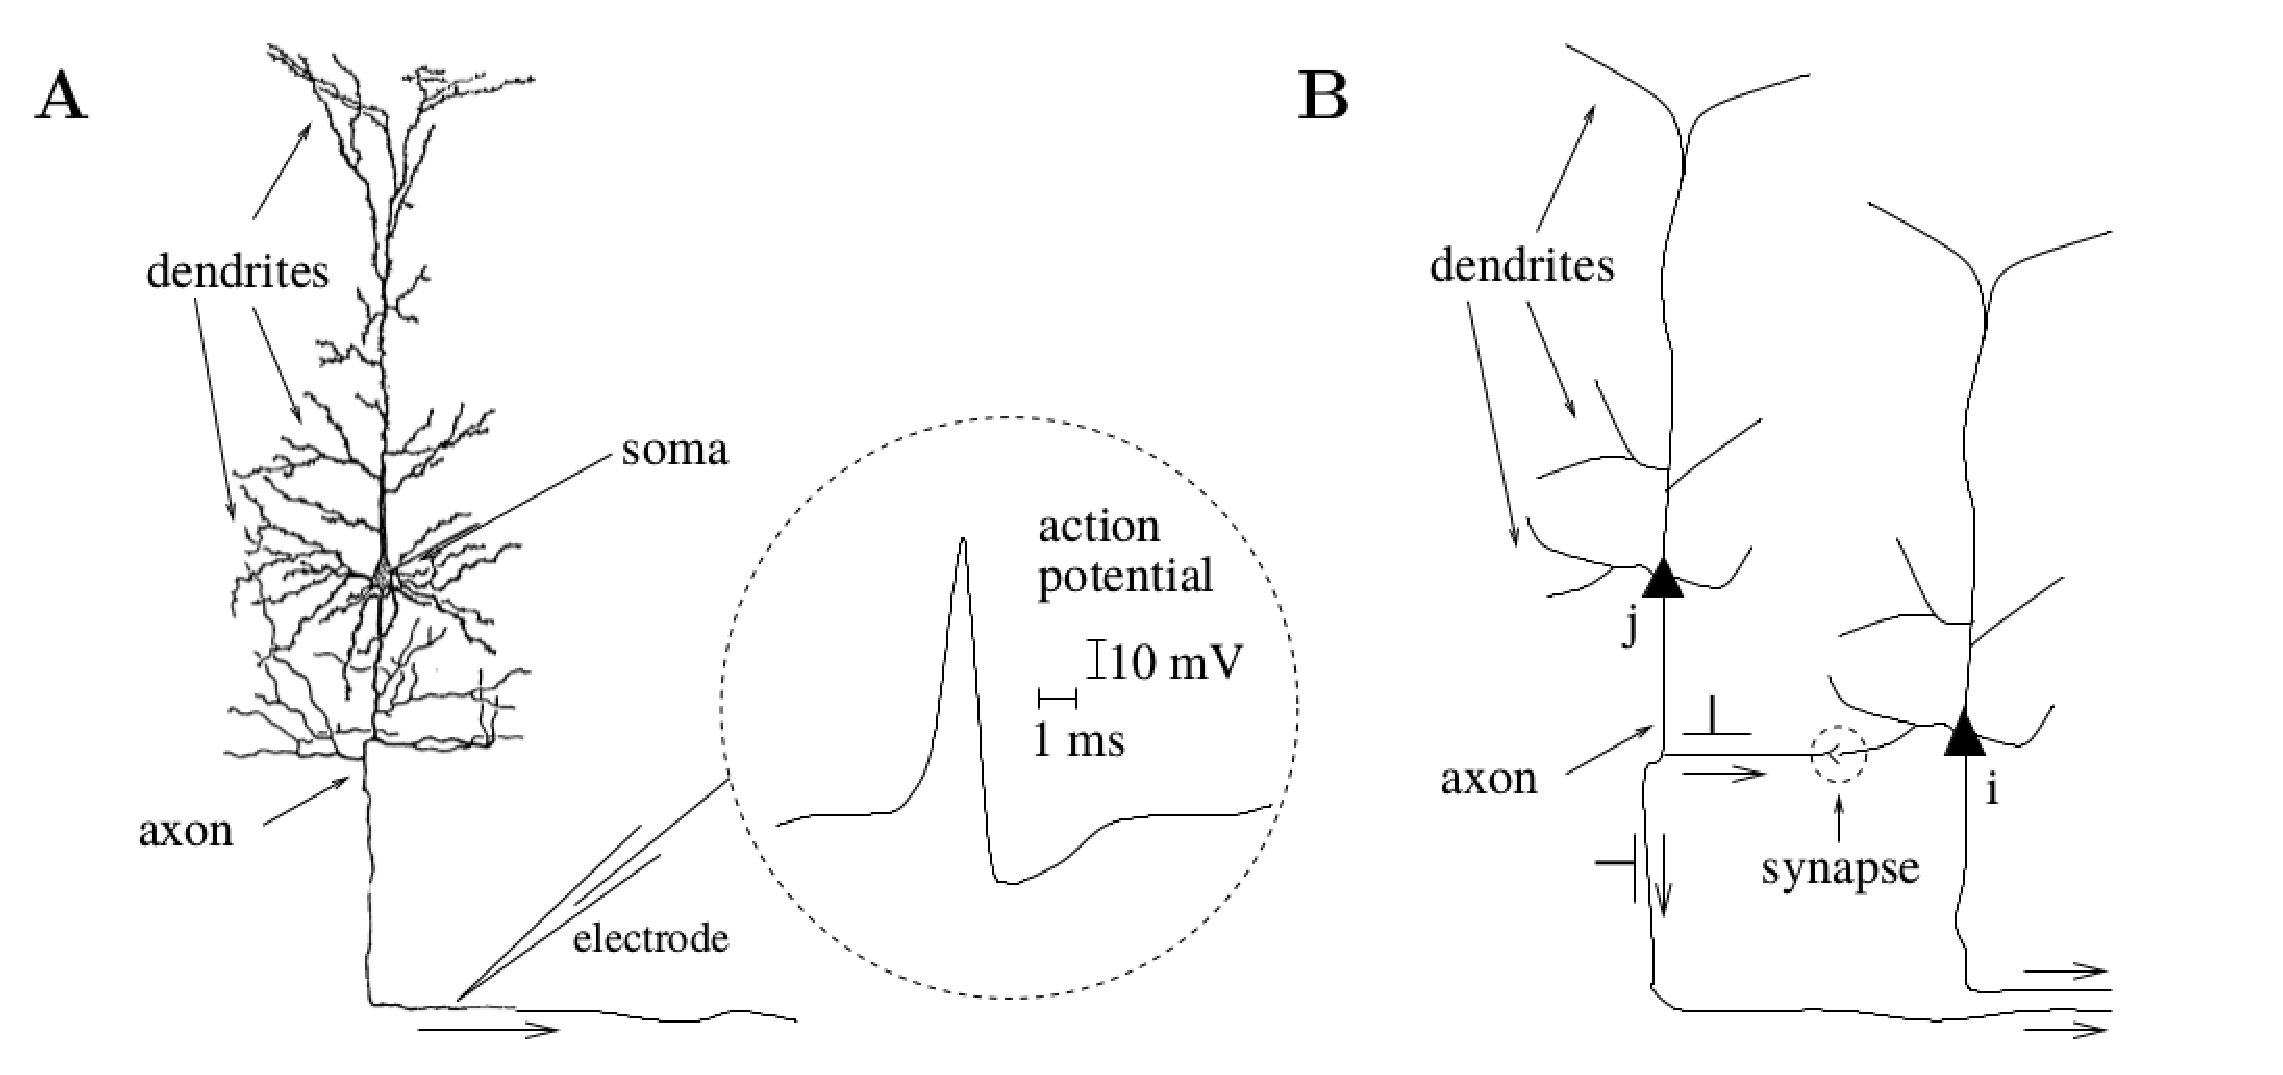
\includegraphics[width=0.85\textwidth]{imgs/Neuron_model.eps}
	\caption{Neuron visualization. Image source \cite{Gerstner2002}}
	\label{fig:biological_neuron}
\end{figure}
Biological neurons exchange information by sending short and sudden pulses, so-called action potentials or spikes.
\todo{include some text here referring to fig \ref{fig:biological_neuron}}
Whenever the membrane potential of a neuron, which can be in- or decreased by incoming spikes depending on the synaptic weight, reaches a certain threshold, the neuron produces a spike itself and resets its membrane potential afterwards \cite{Gerstner2002, Paugam2009}.
Recent neuroscientific research suggests that the exact timing of those spikes encodes information rather than just average firing rates \cite{Bohte2004}.
While traditional \acp{ANN} used in machine learning neglect these biological details, \acp{SNN} embody these spike times and are therefore often referred to as the third generation of neural networks \cite{Maass1997, Paugam2009}.
Maass showed in \cite{Maass1997}, that \acp{SNN} have at least the same computational power as threshold and sigmoidal neural networks of similar size.\\
The simplest spiking neuron model is the \acf{LIF} model with 
\begin{equation}
\frac{\partial V}{\partial t}(t) = - \frac{1}{\tau_{m}} \left( V\left(t\right) - R \cdot I\left(t\right) \right)
\label{eq:LIF}
\end{equation}
\begin{figure}
	\centering
	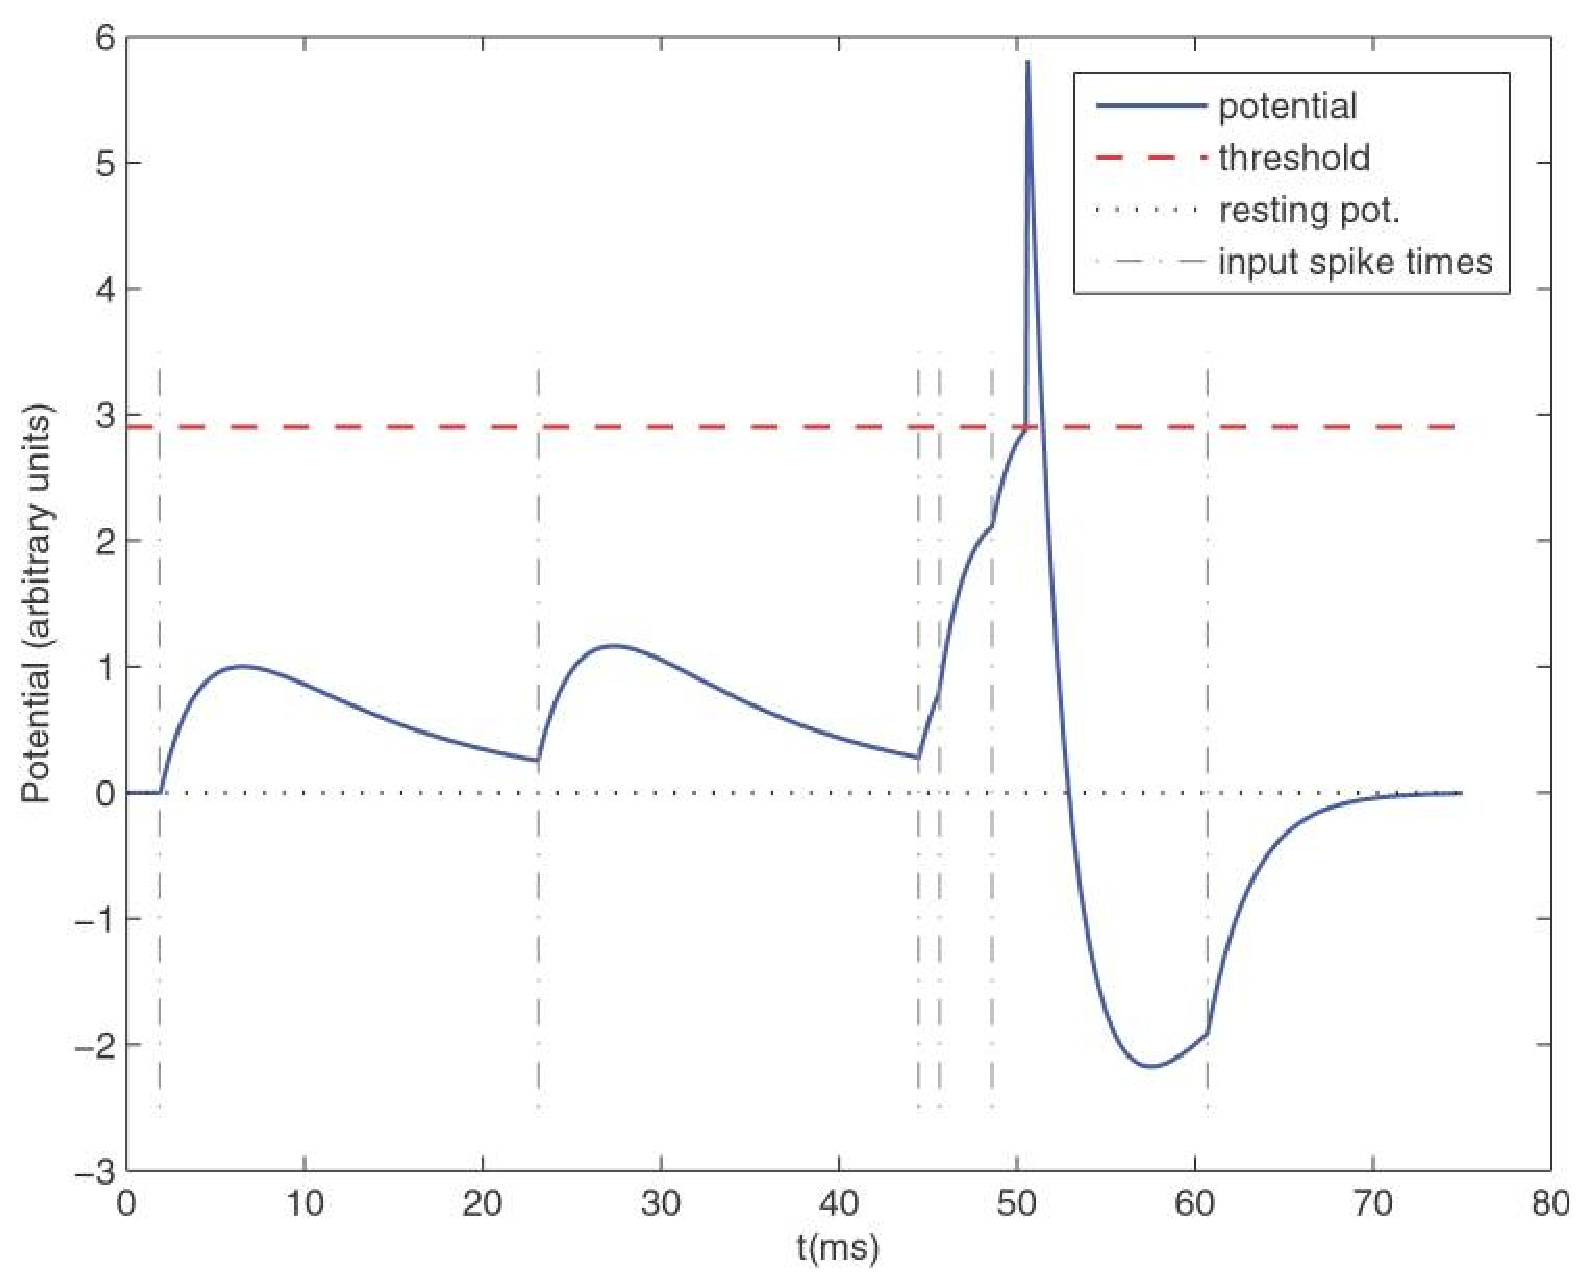
\includegraphics[width=0.75\textwidth]{imgs/LIF_Neuron.eps}
	\caption{Neuron visualization. Image source \cite{Masquelier2007}}
	\label{fig:lif_neuron_model}
\end{figure}
describing the subthreshold behaviour of the neuron, where $V$ is the voltage across the membrane, $I(t)$ is the input current, $R$ is the passive membrane resistance and $\tau_{m}$ is the membrane time constant.
Simply put, equation \ref{eq:LIF} states as follows: the membrane voltage increases in the presence of input current $I(t)$ depending on the membrane resistance $R$ while at the same time, especially in the absence of input current ($I(t)=0$), the voltage decreases or "leaks out" depending on the membrane time constant $\tau_{m}$.
When the voltage $V(t)$ passes a certain threshold $\vartheta$, the neuron produces a spike and the voltage is reset to a resting state $c$ for a certain refractory time interval $\tau_{ref}$ during which incoming spikes have no impact on the membrane potential.
Figure \ref{fig:lif_neuron_model} shows an an example curve of the membrane potential of one \ac{LIF} neuron based on six incoming spikes and visualizes the previously described behaviour. \todo{wording?}
The \ac{LIF} model, despite its biological simplifications, is maybe the most widely used neuron model for simulations due to its simplicity and comparably low computational complexity \cite{Izhikevich2004}, which allows simulations of large networks of neurons in reasonable time.
In contrast, the famous Hodgin-Huxley-model \cite{Hodgkin1952} with its four differential equations and dozens of (biologically meaningful) parameters is the model of high biological plausibility but also computationally challenging regarding large simulations \cite{Izhikevich2004}.
In 2003, Izhikevich proposed a neuron model \cite{Izhikevich2003} as compromise between biological plausibility and computational feasibility.
He showed that this simple model, described by two differential equations with four parameters, is able to produce all known spiking behaviours observed in cortical neurons \cite{Izhikevich2004}. \\
One major hindrance for the widespread adoption of \acp{SNN} has been the problem, that standard learning algorithms for traditional \acp{ANN} like backpropagation \cite{Werbos1974} can not be directly applied to \acp{SNN}.
Although an analogon, the so-called SpikeProp algorithm \cite{Bohte2002} for \acp{SNN} has been developed, the more natural approach is to transfer and mimic biologically inspired learning approaches like Hebbian learning \cite{Hebb1949} or \ac{STDP} \cite{Bi2001}.
An overview of several learning approaches for \acp{SNN} possibly applied with neuromorphic hardware can be found in \cite{Walter2015}.
Another possibility is to train a traditional \ac{ANN} and convert the resulting network into a \ac{SNN} \cite{Diehl2015, Hunsberger2015}.
An example for this approach is the network performing the visual digit recognition task as part of the larger \ac{Spaun} model \cite{Eliasmith2012}, which was derived by training a \ac{DNN} consisting of four \ac{RBM} layers and converting this network using the principles of the \ac{NEF} \cite{Eliasmith2003}.
Although theroretically superior \cite{Maass1997}, \acp{SNN} have not yet outperformed state-of-the-art \acp{DNN} in terms of accuracy in practical machine learning applications \cite{Schmidhuber2015}.\\
Beside the aforementioned procedures to solve traditional machine learning tasks with \acp{SNN} and thereby encode artificial functions in spiking neurons, a different approach is to try to understand how complex cognitive behaviours and the underlying neural functions are performed in the brain.
Therefore, the question how the brain encodes complex information and behaviour in trains of spikes and also how to decode these spike trains to reconstruct the encoded information needs to be answered. 
Although modern research has shed some light on this question regarding the neural code, it is still mainly unanswered as we do not fully understand the anatomical and neurophysiological processes within the brain \cite{Stanley2013}.
Currently, there exist several approaches to code information as spike trains, which can be summarized by the categories rate coding, temporal coding \cite[Chap. 7.6]{Gerstner2014}, population coding \cite[Chap. 1]{Gerstner2002}, \cite{Ponulak2011, Boerlin2011} or sparse coding \cite{Olshausen1996}.
Except for the biologically unrealistic rate coding approach, there are cues for all of these coding schemes and even combinations \cite{Gupta2014} of them to appear in biological systems.

%----------------------------------------------------------------------------------------------------------
\subsection{Neural Engineering}
\label{subsec:neural_eng}
%----------------------------------------------------------------------------------------------------------
In this section, we give a brief overview of the \acf{NEF}, as we will be making use of it in forthcoming chapters.
The \ac{NEF} \cite{Eliasmith2003} is a mathematical theory, which provides a set of methods to construct biologically plausible, large-scale neural models.
These methods can be divided into the three main principles of the \ac{NEF}: \emph{representation}, \emph{transformation} and \emph{dynamics}.
The \ac{Nengo} \cite{Bekolay2014, Nengo} software suite is a python library, which implements the \ac{NEF}'s principles.
\ac{Nengo} has been used to build a variety of neural models, e.g. models of the basal ganglia system \cite{Stewart2010, Stewart2012} and \acf{Spaun} \cite{Eliasmith2012}, a large-scale, functional model of the brain, which is able to perform eight cognitive tasks.
Furthermore, \ac{Nengo} has been used to interface neural models with physical, neuromorphic hardware systems and robots \cite{Conradt2014, Stewart2016, Mirus2018a}.
Here, we give a brief introduction to the \ac{NEF}'s principles and refer to \cite{Eliasmith2003, Eliasmith2013, Bekolay2014} for more details.
\subsubsection{Representation}
\label{subsubsec:nef_representation}
The first principle of the \ac{NEF}, representation, provides mathematical tools to encode information, namely time-varying real-valued vectors, in the activity of neural populations.
It is based on the assumption, that neurons have a "preferred direction vector" in the represented space, each neuron responds most strongly to.
This assumption is grounded by the findings of \cite{Georgopoulos1989} that each neuron in motor cortex of rhesus monkeys has a different preferred arm direction.
The \ac{NEF} expands this idea to neural representations in general.
\begin{figure}[t!]
	\centering
	\subfloat[Tuning curves \label{subfig:nef_rep_tuning_curves}]{%
		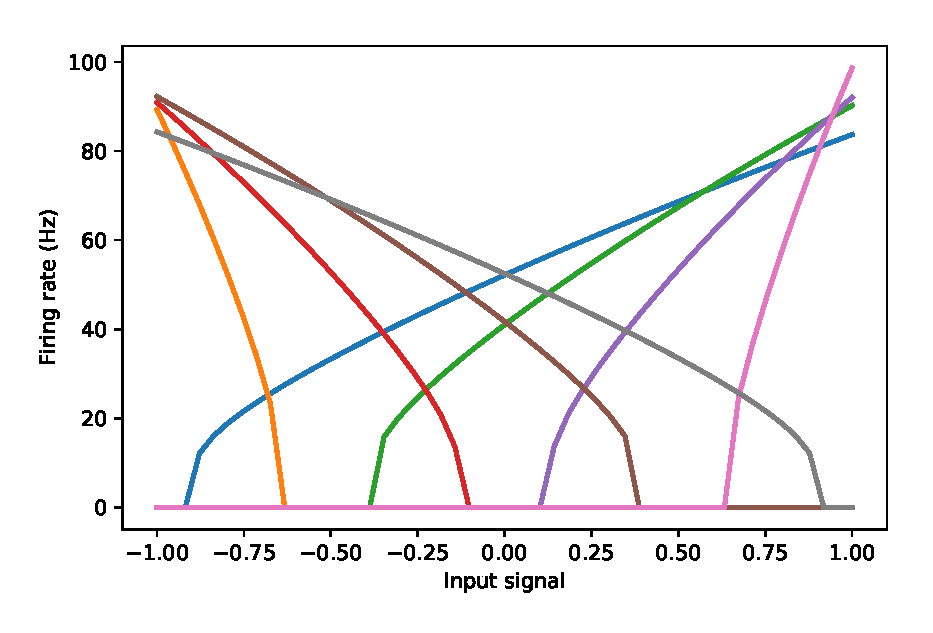
\includegraphics[width=0.45\textwidth]{imgs/NEF_tuning_curves.eps}
	}
	\subfloat[Spike times\label{subfig:nef_rep_spike_raster}]{%
		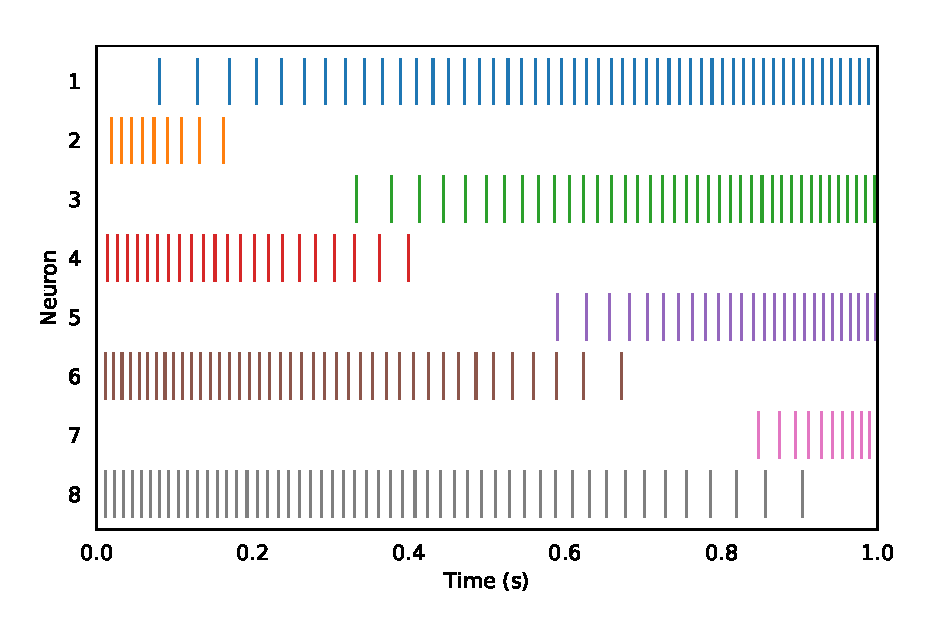
\includegraphics[width=0.45\textwidth]{imgs/NEF_spikes_raster.eps}
	}\\
	\vspace{-0.4cm}
	\subfloat[Decoded output\label{subfig:nef_rep_decoded}]{%
		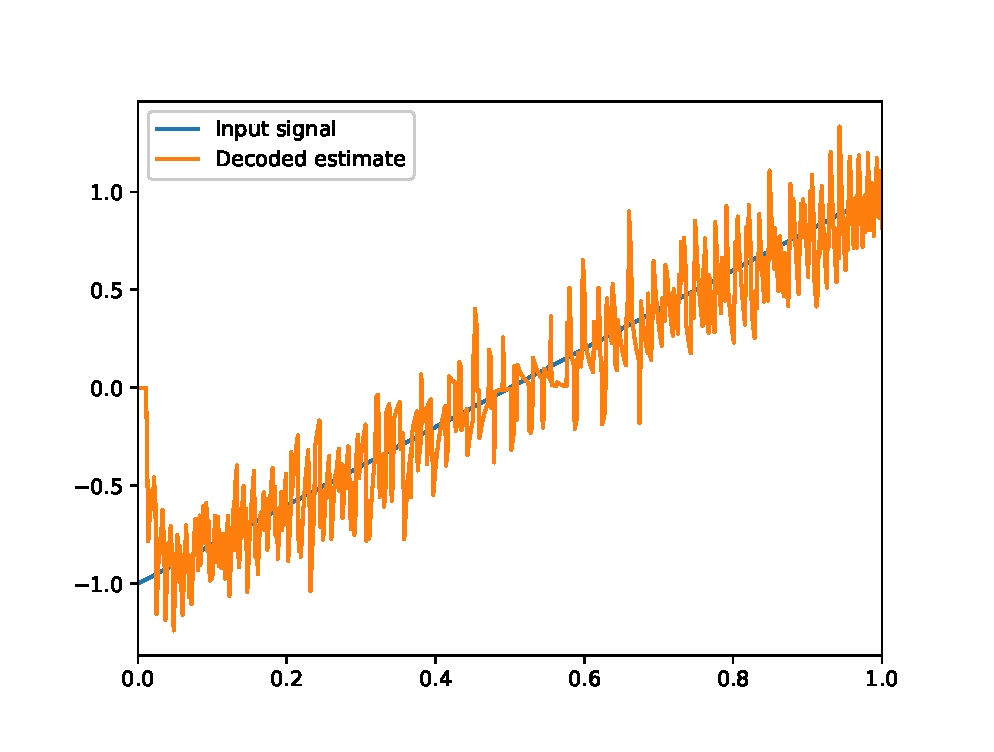
\includegraphics[width=0.45\textwidth]{imgs/NEF_decoded_output.eps}
	}
	\subfloat[Filtered neural activity\label{subfig:nef_rep_spike_filtered}]{%
		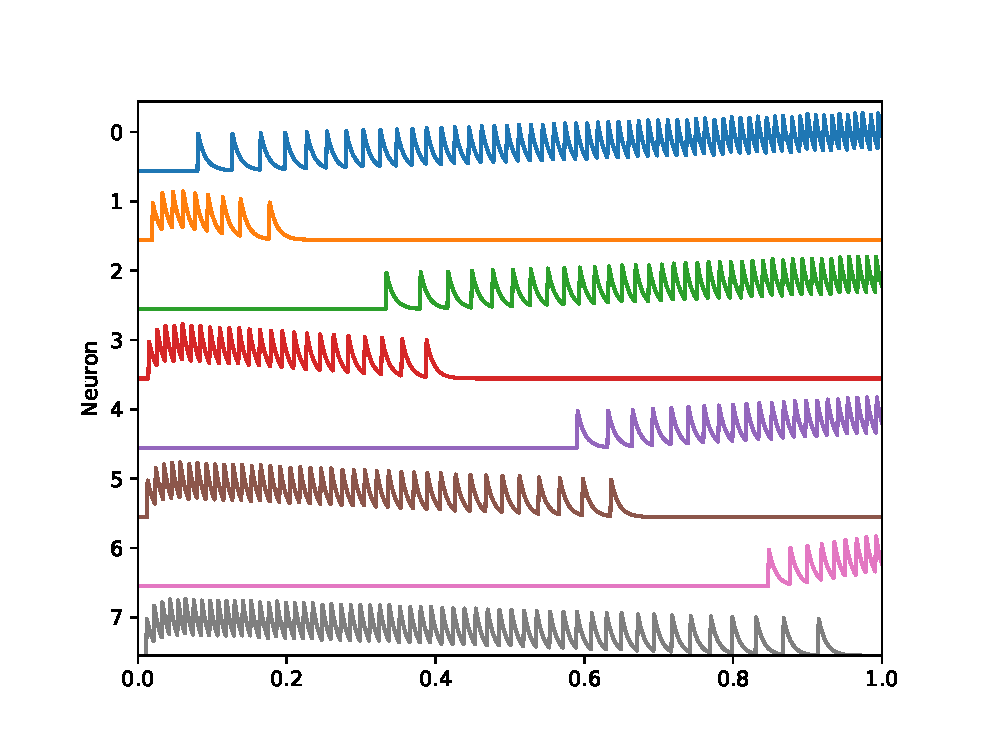
\includegraphics[width=0.45\textwidth]{imgs/NEF_spikes_filtered.eps}
	}
	\caption{The representation principle of the \ac{NEF}. Images adapted from \cite{Bekolay2014}}\label{fig:nef_representation}
\end{figure}
Let $A$ be a population of $N \in \mathbb{N}$ neurons encoding a subset $V$ of a real-valued vector space, i.e. $V\subseteq \mathbb{R}^{n}$.
Given a function $\abbil{\mathbf{x}}{\mathbb{R}}{V}$, we can write the activity $a_{i}$ of the $i$-th neuron in a neural population encoding a time-varying vector $\mathbf{x}(t)$ as a spike train, i.e. a sum of delta functions
\begin{equation}
a_{i}\left(\mathbf{x}(t)\right) = \sum_{j=1}^{m_{i}} \delta(t - t_{j}) = G_{i}(\underbrace{\alpha_{i}\langle\mathbf{e}_{i},\mathbf{x}(t)\rangle + J_{i}}_{=:c}) \quad \textrm{ for } 1 \leq i \leq N, 
\label{eq:nef_encoding}
\end{equation}
where $G_{i}$ is the spiking neural non-linearity, $\alpha_{i}$ is the gain of the neuron, $\mathbf{e}_{i}$ is the neuron's preferred direction or encoding vector and $J_{i}$ is a bias current to account for neural background activity and $t_{j}$ are the $m{i}$ spike-times of the $i$-th neuron.
Notably, the current flowing into the cell is completely determined by $c$, whereas the spiking behaviour of the neuron model is represented by the non-linear function $G_{i}$.
The input current $c$ and therefore the \ac{NEF}'s encoding process is independent of particular spiking neuron models.\\
To decode the input values $\mathbf{x}(t)$ back out of the neural population $A$, the spike train is convolved with an exponentially decaying filter $\abbil{h}{\mathbb{R}}{\mathbb{R}}$ to simulate the process of neurons generating postsynaptic current after spiking (cf. fig. \ref{subfig:nef_rep_spike_filtered}) resulting in
\begin{equation}
\tilde{a}_{i}\left(\mathbf{x}(t)\right) = \sum_{j=1}^{m_{i}} h(t) \ast \delta(t - t_{j}) = \sum_{j=1}^{m_{i}} h(t - t_{j}).
\label{eq:nef_filtered_activity}
\end{equation}
A simple model of an exponential decaying filter is the function $\abb{h}{\mathbb{R}}{\mathbb{R}}{t}{e^{\sfrac{-t}{\tau_{p}}}}$, where $\tau_{P}$ denotes the postsynaptic time constant.
We obtain an estimation $\mathbf{\hat{x}}(t)$ of the original input $\mathbf{x}(t)$ as a weighted sum with some decoder values $\mathbf{d}_{i}$
\begin{equation}
\mathbf{\hat{x}}(t) = \sum_{i=1}^{N} \tilde{a}_{i}\left(\mathbf{x}(t)\right) \mathbf{d}_{i}.
\label{eq:nef_decoding} 
\end{equation} 
To calculate the optimal decoders $\mathbf{d}_{i}$, we need to minimize the error between input $\mathbf{x}(t)$ and decoded output $\mathbf{\hat{x}}(t)$
\begin{equation}
E = \int \left( \mathbf{x}(t) - \sum_{i=1}^{N} \tilde{a}_{i}\left(\mathbf{x}(t)\right) \mathbf{d}_{i}\right)^{2} \diff \mathbf{x}(t).
\label{eq:decoder_calculation}
\end{equation}
\ac{Nengo} solves for the decoders $\mathbf{d}_{i}$ by default using least squares optimization \cite{Eliasmith2013}[Appendix B1].
Fig. \ref{fig:nef_representation} visualizes this encoding process for $V = \left[ -1, 1\right] \subset \mathbb{R}$ and a population of $8$ neurons.
Fig. \ref{subfig:nef_rep_tuning_curves} shows the tuning curves of individual neurons, which define how these neurons respond to specific input values.
Equation \ref{eq:nef_encoding} is depicted in fig. \ref{subfig:nef_rep_spike_raster}, which shows a raster plot of the neurons' spike times based on the input signal shown in fig. \ref{subfig:nef_rep_decoded}.
Fig. \ref{subfig:nef_rep_spike_filtered}, which shows the filtered neural activity for each neuron, visualizes equation \ref{eq:nef_filtered_activity}.
Finally, fig. \ref{subfig:nef_rep_decoded} depicts the original input value as well as the estimated output of the neural populations' activity (cf. equation \ref{eq:nef_decoding}).
Note, that the neural population's decoded output is only a noisy approximation of the original input value, whose accuracy can be improved by increasing the number of neurons in the population.
\subsubsection{Transformation}
\begin{figure}[t]
	\centering
	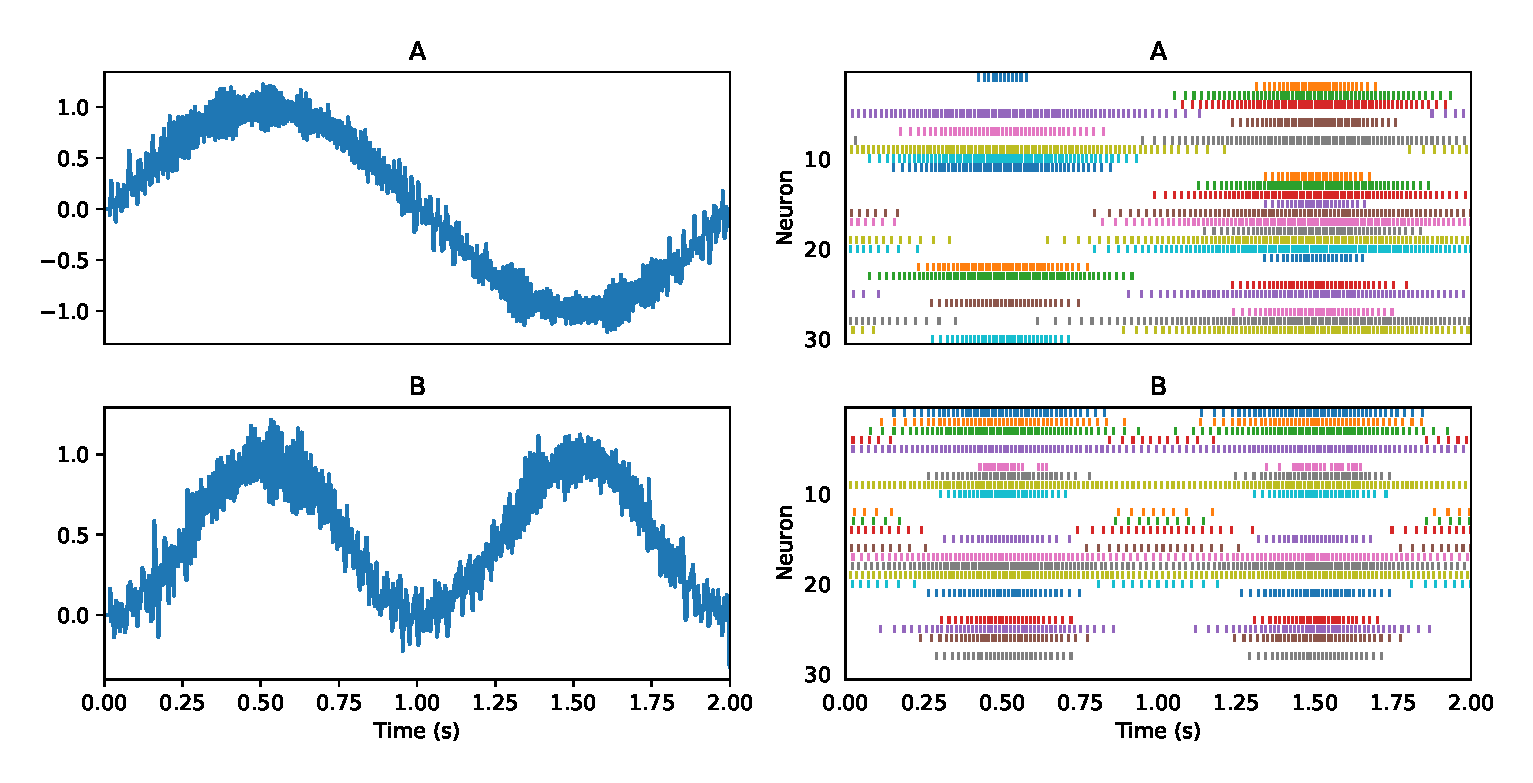
\includegraphics[width=0.85\textwidth]{imgs/NEF_transformation.eps}
	\caption{The transformation principle of the \ac{NEF}.}
	\label{fig:nef_transformation}
\end{figure}
The second main principle of the \ac{NEF}, \emph{transformation}, provides the mathematical tools to compute functions across conncetions between populations of neurons.
Let $A$ resp. $B$ be populations of $N$ resp. $M$ neurons encoding a time-varying vector $\mathbf{x}(t) \in V \subset \mathbb{R}^{n}$ resp. $\mathbf{y}(t) \in W \subset \mathbb{R}^{m}$ according to the representation principle and a function $\abbil{f}{V}{W \subset \mathbb{R}^{m}}$.
In order to approximate the funtion $f$ across a connection from population $A$ to population $B$, we use the tools of the representation principle, but we calculate a different set of decoder values $\mathbf{d}_{i}^{f}$ for population $A$ by minimizing the error
\begin{equation}
\label{eq:nef_transformation}
E = \int \left( f(\mathbf{x}(t)) - \sum_{i=1}^{N} \tilde{a}_{i}\left(\mathbf{x}(t)\right) \mathbf{d}_{i}^{f}\right)^{2} \diff \mathbf{x}(t).
\end{equation}
Given encoders $\mathbf{e}_{j}^{B}$ and gain $\alpha_{j}^{B}$ for $1 \leq j \leq M$ of population $B$, we can derive a weight matrix for the connection from $A$ to $B$ approximating the function $f$ by
\begin{equation}
w_{ij} = \alpha_{j}^{B} \mathbf{d}_{i}^{f} L \mathbf{e}_{j}^{B} \quad \textrm{for } 1 \leq i \leq N \textrm{ and } 1 \leq j \leq M, 
\end{equation}
where $L$ is a $M \times N$ linear operator. 
Here, the \ac{NEF} makes the assumption, that connection weights can be factored into encoders, decoders and a linear transform.
Fig. \ref{fig:nef_transformation} visualizes this \ac{NEF}'s transformation principle for $V = W = \left[ -1, 1\right] \subset \mathbb{R}$, two neural populations $A$, $B$ containing $30$ neurons each.
The left resp. right panel of plots shows the populations' decoded outputs resp. the neurons' spike times.
Population $A$ uses the representation principle to encode a sine function, whereas the transformation principle was used to calculate the function $\abb{f}{V}{W}{x}{f(x)=x^{2}}$ across the connection from $A$ to $B$.

\subsubsection{Dynamics}
\begin{figure}[t]
	\centering
	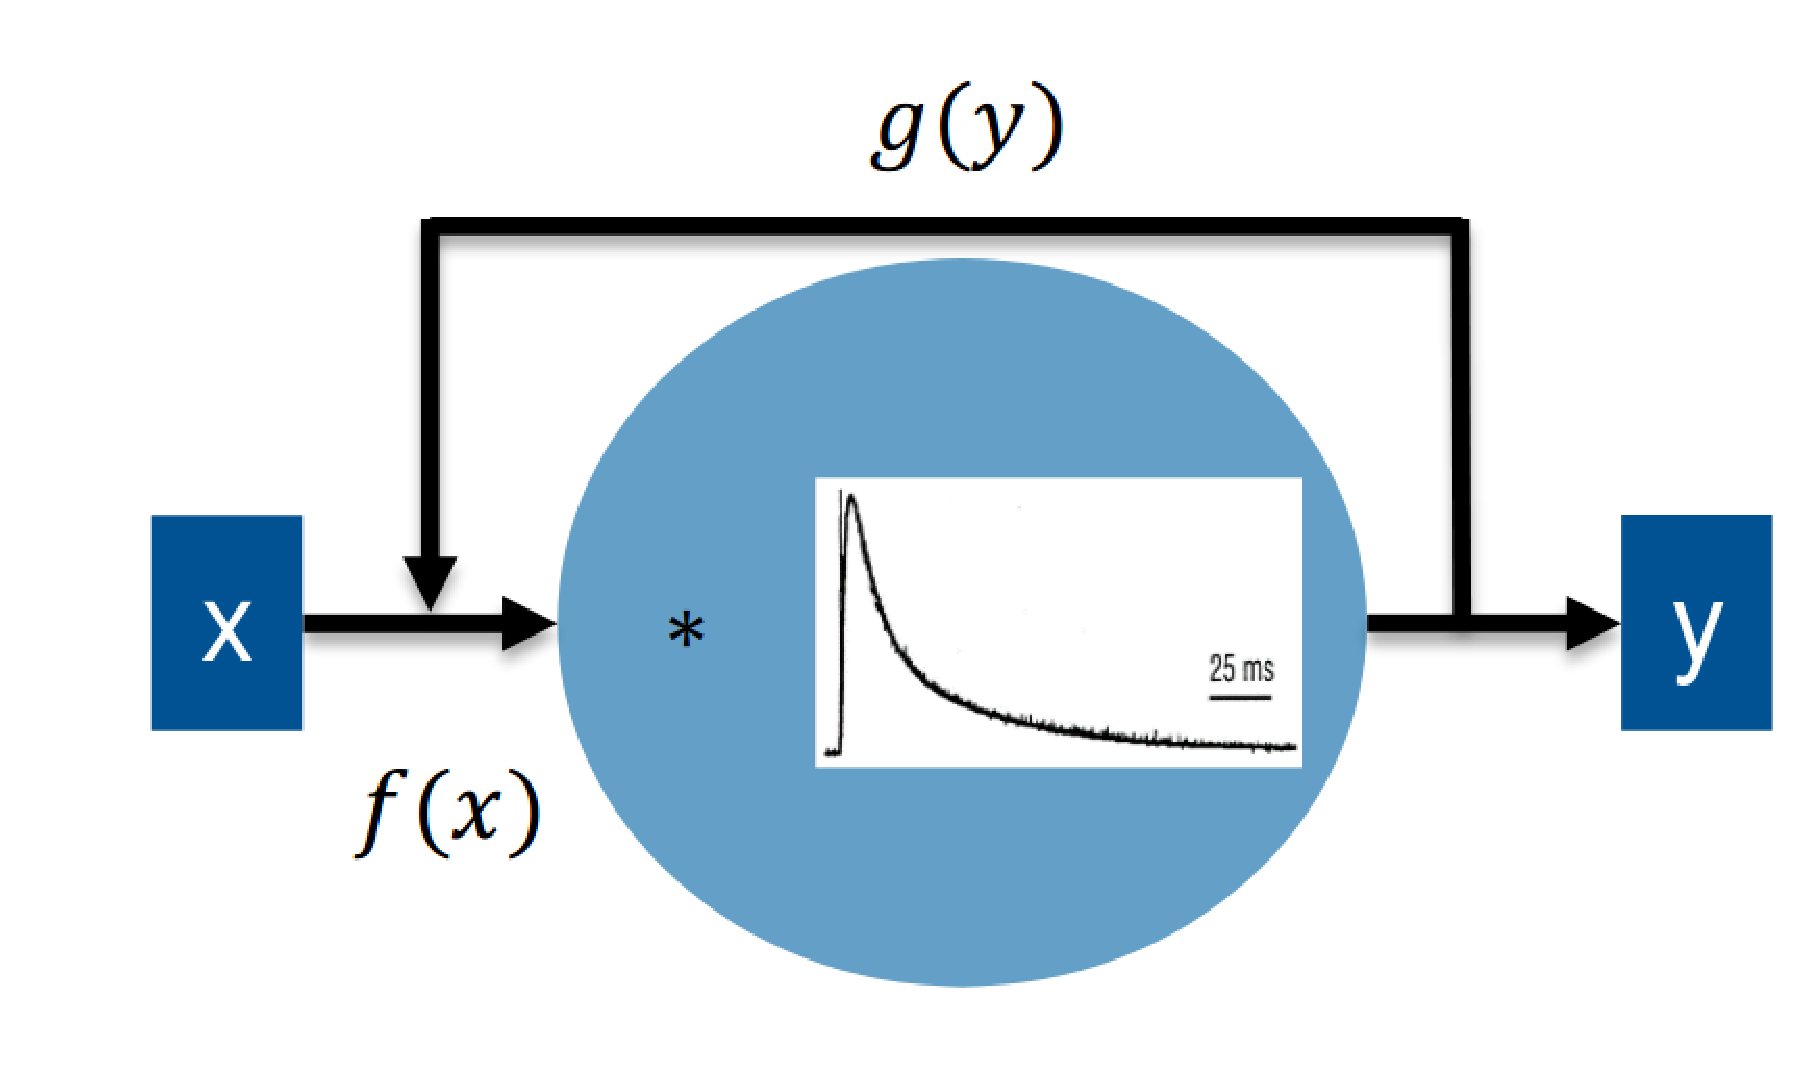
\includegraphics[width=0.85\textwidth]{imgs/NEF_recurrent.eps}
	\caption{The dynamics principle of the \ac{NEF} for recurrent connections. \todo{make a better figure!}}
	\label{fig:nef_dynamics}
\end{figure}
The third main principle of the \ac{NEF}, \emph{dynamics}, provides a set of mathematical tools to implement dynamical systems in neural populations through recurrent connections.
Let $A$ be a population of neurons with an incoming connection approximating the function $\abbil{f}{V}{W \subset \mathbb{R}^{m}}$ and a recurrent connection approximating the function $\abbil{g}{W}{W}$ (cf. fig. \ref{fig:nef_dynamics}).
Thus, the overall function the population is approximating is 
\begin{equation}
\mathbf{y}(t) = h(t) \ast \left(f(\mathbf{x}(t)) + g(\mathbf{y}(t))\right)
\label{eq:nef_dyn}
\end{equation}
with exponential decaying filter function $\abb{h}{\mathbb{R}}{\mathbb{R}}{t}{e^{\sfrac{-t}{\tau}}}$.
By applying the Laplace transform to equation \ref{eq:nef_dyn}, we get
\begin{equation}
\label{eq:nef_dyn_laplace}
\mathbf{Y}(s) = \frac{1}{1 + s\tau}\left(F(\mathbf{X}(s)) + G(\mathbf{Y}(s))\right).
\end{equation}
We can rearrange equation \ref{eq:nef_dyn_laplace} to
\begin{equation}
s\mathbf{Y}(s) = \frac{G(\mathbf{Y}(s))-\mathbf{Y}}{\tau} + \frac{F(\mathbf{X}(s))}{\tau}.
\end{equation}
Transforming back leads to the differential equation
\begin{equation}
\frac{\partial \mathbf{y}(t)}{\partial t} = \frac{g(\mathbf{y}(t)-y)}{\tau} + \frac{f(\mathbf{x}(t))}{\tau}.
\end{equation}
Thus, to construct a neural model approximating a differential equation of the form 
\begin{equation}
\frac{\mathbf{y}(t)}{\partial t} = a(\mathbf{y}(t)) + b(\mathbf{x}(t))
\label{eq:nef_dyn_diffeq}
\end{equation}
with functions $\abbil{a}{W}{W}$ and $\abbil{b}{V}{W}$, the first two principles of the \ac{NEF} can be used to create a neural population of the form as shown in fig. \ref{fig:nef_dynamics}.
By setting the functions $g(\mathbf{y}(t))=\tau a(\mathbf{y}(t)) + \mathbf{y}(t)$ and $f(\mathbf{x}(t))=\tau b(\mathbf{x}(t))$, we obtain a neural model approximating the desired dynamical system described by the differential equation \ref{eq:nef_dyn_diffeq}.
%The term "neuromorphic" was first introduced by Carver Mead in \cite{Mead90}, when describing one of the first silicon retinas.
%For clarity, a first broad definition is provided, which will need some refinement while proceeding in this section:
%\begin{defn}
%\label{def:neuromorph}
%Artificial systems, that share organization principles with biological nervous systems are called \textbf{neuromorphic}.
%\end{defn} 
%Biologically inspired systems and algorithms have seen significant progress and achieved remarkable results, e.g. in the field of machine learning, despite some simplifications in terms of biological accuracy.
%So-called first and second generation \ac{ANN} described in \ref{subsec:ML_ANN} are also covered by definition \ref{def:neuromorph} as neuromorphic systems, although they neglect some biological details.
%\subsection{Spiking Neural Networks}
%Biological neurons exchange information by sending short and sudden increases in their membrane voltage, so-called action potentials or spikes.
%Recent neurological research suggests that the exact timing of those spikes encodes information rather than just average firing rates (\todo{Citation}).
%While \ac{ANN} of the first two generations neglect these biological details, recent neural networks structures, so-called \ac{SNN} \cite{Paugam2009}, embody these spike times and are therefor often referred to as the third generation of neural networks . 
%
%
%
%\label{subsec:spiking_neural_nets}
%
%\subsection{Neural Modelling}
%\subsection{Neuromorphic Hardware}
%The field of neuromorphic computing achieved several significant advances in recent years, massively increasing the number of neurons simultaneously available in complex models and achieving real-time (less than $\SI{100}{\milli\second}$) execution through hardware implementation. 
%This basic research is resulting in semiconductor implementations becoming available on a wider scale, such as University of Manchester's \ac{SpiNNaker} Chip \cite{Furber2014} or IBM’s recently announced True North \cite{Akopyan2015} architecture.
%\section{Traditional Computing}

\section{\aclp{VSA}}
The term \acfp{VSA} - first coined by Ross W. Gayler \cite{Gayler2003} - refers to a class of similar approaches for cognitive modeling making use of distributed representations.
The basic idea behind all of those approaches is to represent structure (e.g. cognitive concepts, symbols or language) in a high-dimensional vector space by mapping each entity to be represented to a (possibly random) vector.
One of the most important properties of high-dimensional vector spaces enabling this kind of representation is the fact, that two high-dimensional random vectors are likely to be dissimilar.
In the following, we will show what we mean by fuzzy terms like \emph{dissimilar} or \emph{likely} and provide more precise statements.\\
One main requirement in the context of cognitive modeling is the ability of the modeling framework to address the binding problem \cite{Treisman1999}.
In \cite{Jackendoff2002}, Jackendoff phrases this as the problem of "combining independent bits into a single coherent percept". 
One strength of \acp{VSA} is that they offer the possibility to manipulate their entities (i.e. vectors) through algebraic operations, usually at least one \emph{addition-like} and \emph{multiplication-like} operation each.
Typically, the multiplication operation is used for binding different representations into a new vector.
This operation, depending on the vector representation, is constructed with some desirable properties in mind (see Definition \ref{def:binding}).
A first attempt on using a multiplication operation on vectors for binding was done by Smolensky \cite{Smolensky1990} using the tensor product.
The major drawback of this approach is exploding dimensionality of the tensor product.
For finite dimensional vector spaces  $V$ and $W$ of dimensions $n$ and $m$, the tensor space $V \otimes W$ is a vector space of dimension $n\cdot m$.
As a consequence, each binding operation $v\otimes w$ for vectors $v \in V, w \in W$ would increase the dimension of the representational space, which is computationally infeasible and leads to poor scaling.
This lead researchers to define several slightly different multiplication or binding operations, depending on the underlying numerical structure.
The most prominent examples are elementwise multiplication in Gayler's \ac{MAP}-architecture \cite{Gayler1998}, the XOR-operation in Kanerva's \acp{BSC} \cite{Kanerva2000, Kanerva2009} as well as circular convolution in Plate's \acp{HRR} \cite{Plate1991, Plate1994}.

\subsection{Mathematical properties of \aclp{VSA}}
%Before we provide a formal definition for \acp{VSA}, we introduce some terms and auxiliary tools needed for later use.
%\begin{defn}
%	\label{def:metric}
%	Let $M$ be a set. A function 
%	\[
%	\abb{d}{M \times M}{\mathbb{R}}{(x,y)}{d(x,y)} 
%	\]
%	is called a \emph{metric}, if and only if for any $x, y \in M$ the following conditions hold:
%	\begin{enumerate}
%		\item $d(x,y) \geq 0$ (non-negativity)
%		\item $d(x,y) = 0 \Longleftrightarrow x = y$ (identity of indiscernibles)
%		\item $d(x,y) = d(y,x)$ (symmetry)
%		\item $d(x,z) \leq d(x,y) + d(y,z)$ (triangle inequality)
%	\end{enumerate}
%	We call the ordered pair $(M,d)$ a \emph{metric space}.
%\end{defn}


\begin{defn}
	\label{def:VSA}
	Let $N \subseteq K$ be a subset of some number field $K$ (ie.e a set of numbers) and $D \in \mathbb{N}$ a natural number. 
	Furthermore, let 
	\[V_{D}(N)=\{\left(x_{0}, \cdots, x_{D-1}\right)  | x_{i} \in N\} \subseteq K^{D}\] 
	be the set of all $D$-tuples with entries in $N$. 
	Let
	\begin{align*}
	&\abb{\oplus}{V_{D}(N) \times V_{D}(N)}{K^{D}}{(v,w)}{\oplus(v,w) =: v\oplus w}, \\
	&\abb{\varoast}{V_{D}(N) \times V_{D}(N)}{K^{D}}{(v,w)}{\varoast(v,w) =: v\varoast w}
	\end{align*}
	be functions with $\oplus$ following the rules of ordinary addition - namely commutativity, associativity, existence of a neutral element and existence of inverse elements - and for any elements $u,v,w \in V_{D}(N)$
	\[u \varoast (v \oplus w) = u \varoast v \oplus u \varoast w.\]
	If there is furthermore a distinct element $\pmb{1} \in V_{D}(N)$ with 
	\[v \varoast \pmb{1} = \pmb{1} \varoast v = v\]
	for any $v \in V_{D}(N)$ and a function $\abbil{\phi}{V_{D}(N) \times V_{D}(N)}{\left[-1,1\right]}$, we call $(V_{D}(N), \varoast, \oplus, \phi)$ a \emph{\acrfull{VSA}} of dimension $D$.
	The function $\phi$ is called a \emph{measure of similarity}.
	If $N$ is a subset of the real or complex numbers, i.e. $N \subset \mathbb{R}$ or $N \subseteq \mathbb{C}$, we call any \ac{VSA} $\left(V_{D}(N), \varoast, \oplus, \phi\right)$ \emph{continuous}.
\end{defn}
Although the set $V_{D}(N)$ might not be a vector space in the strict mathematical sense (in most cases it is at least a subset of a vector space), we will refer to its elements as \emph{vectors}.
\todo{note that VSA in general must not be closed under its operations}
%The metric in definition \ref{def:VSA} is needed as measure of similarity between vectors. 
Before we proceed in deriving some important properties of \acp{VSA}, we present some of the most prominent examples.

\begin{ex} \aclp{VSA}
	\label{ex:VSAs}
	\begin{enumerate}
		\item The first example of a \ac{VSA} is Kanerva's \acfl{BSC} \cite{Kanerva2009}. 
		He restricts the elements of his vectors to binary values, i.e. $N=\{0,1\}$
		The operations $\varoast$ and $\oplus$ in this case are the XOR-function and a thresholded sum respectively.
		With $v_{i} = \left(v_{i 0}, \cdots, v_{i D-1}\right) \in V_{D}(N)$ and  $i \in \{1, \cdots, n\}$, the operation $\oplus$ is usually defined in the following way
		\begin{align*}
		v_{1} \oplus \cdots \oplus v_{n} =: &x = \left(x_{0}, \cdots, x_{D-1}\right) \textrm{ with } \\
		&x_{j}:= \begin{cases}
		1 & \sum\limits_{i=1}^{n} v_{ij} \geq \frac{n}{2} \\
		0 & \sum\limits_{i=1}^{n} v_{ij} < \frac{n}{2}
		\end{cases}.
		\end{align*}
		This definition ensures, that the results of the addition operation $\oplus$ remain binary.
		Usually, a normalized Hamming distance 
		\[
		\phi(v,w) := 1 - \frac{2}{D} \left| \{ v_{i} \neq w_{i} | i \in \{0, \cdots, D-1\} \} \right|
		\]
		is used as a measure of similarity in this architecture.
		\acp{BSC} have some interesting properties compared to other \acp{VSA}: 
		The neutral element for both operations $\varoast$ and $\oplus$ is the vector $\pmb{0} := \left(0, \cdots, 0\right)$, while all vectors are self-inverse regarding the multiplication operation $\varoast$, i.e. $v \varoast v = \pmb{0}$ for any $v \in V_{D}(N)$.
		
		\item The first example of \ac{VSA} in continuous space is Gayler's \acrfull{MAP} architecture \cite{Gayler1998} with $N \subseteq \mathbb{R}$ and the cosine simlarity as measure of similarity 
		\[
		\phi(v,w) = \frac{v \cdot w}{\norm{v}\norm{w}}=\cos(\theta),
		\]
		with $\theta$ being the angle between the vectors $v,w \in V_{D}(N)$.
		The operations $\varoast$ and $\oplus$ are simply element-wise multiplication and addition with neutral elements $\pmb{1}=\left(1, \cdots, 1\right)$ and $\pmb{0} := \left(0, \cdots, 0\right)$ respectively.
		
		\item Another example of a \ac{VSA} in continuous space is Plate's \acfl{HRR} \cite{Plate1994, Plate1997}.
		The main difference compared to the \ac{MAP} architecture is, that Plate in general allows complex vector values, i.e. $N \subseteq \mathbb{C}$ and uses a different multiplication operation $\varoast$ - namely circular convolution.
		For any two vectors $x, y \in V_{D}(N)$, circular convolution $\varoast$ is defined as
		\begin{align*}
		z = v \varoast w \qquad \textrm{ with } z_{j} := \sum_{k=0}^{D-1} x_{k}y_{(j-k)\Mod{D}}.
		\end{align*}
		\begin{figure}
			\centering
			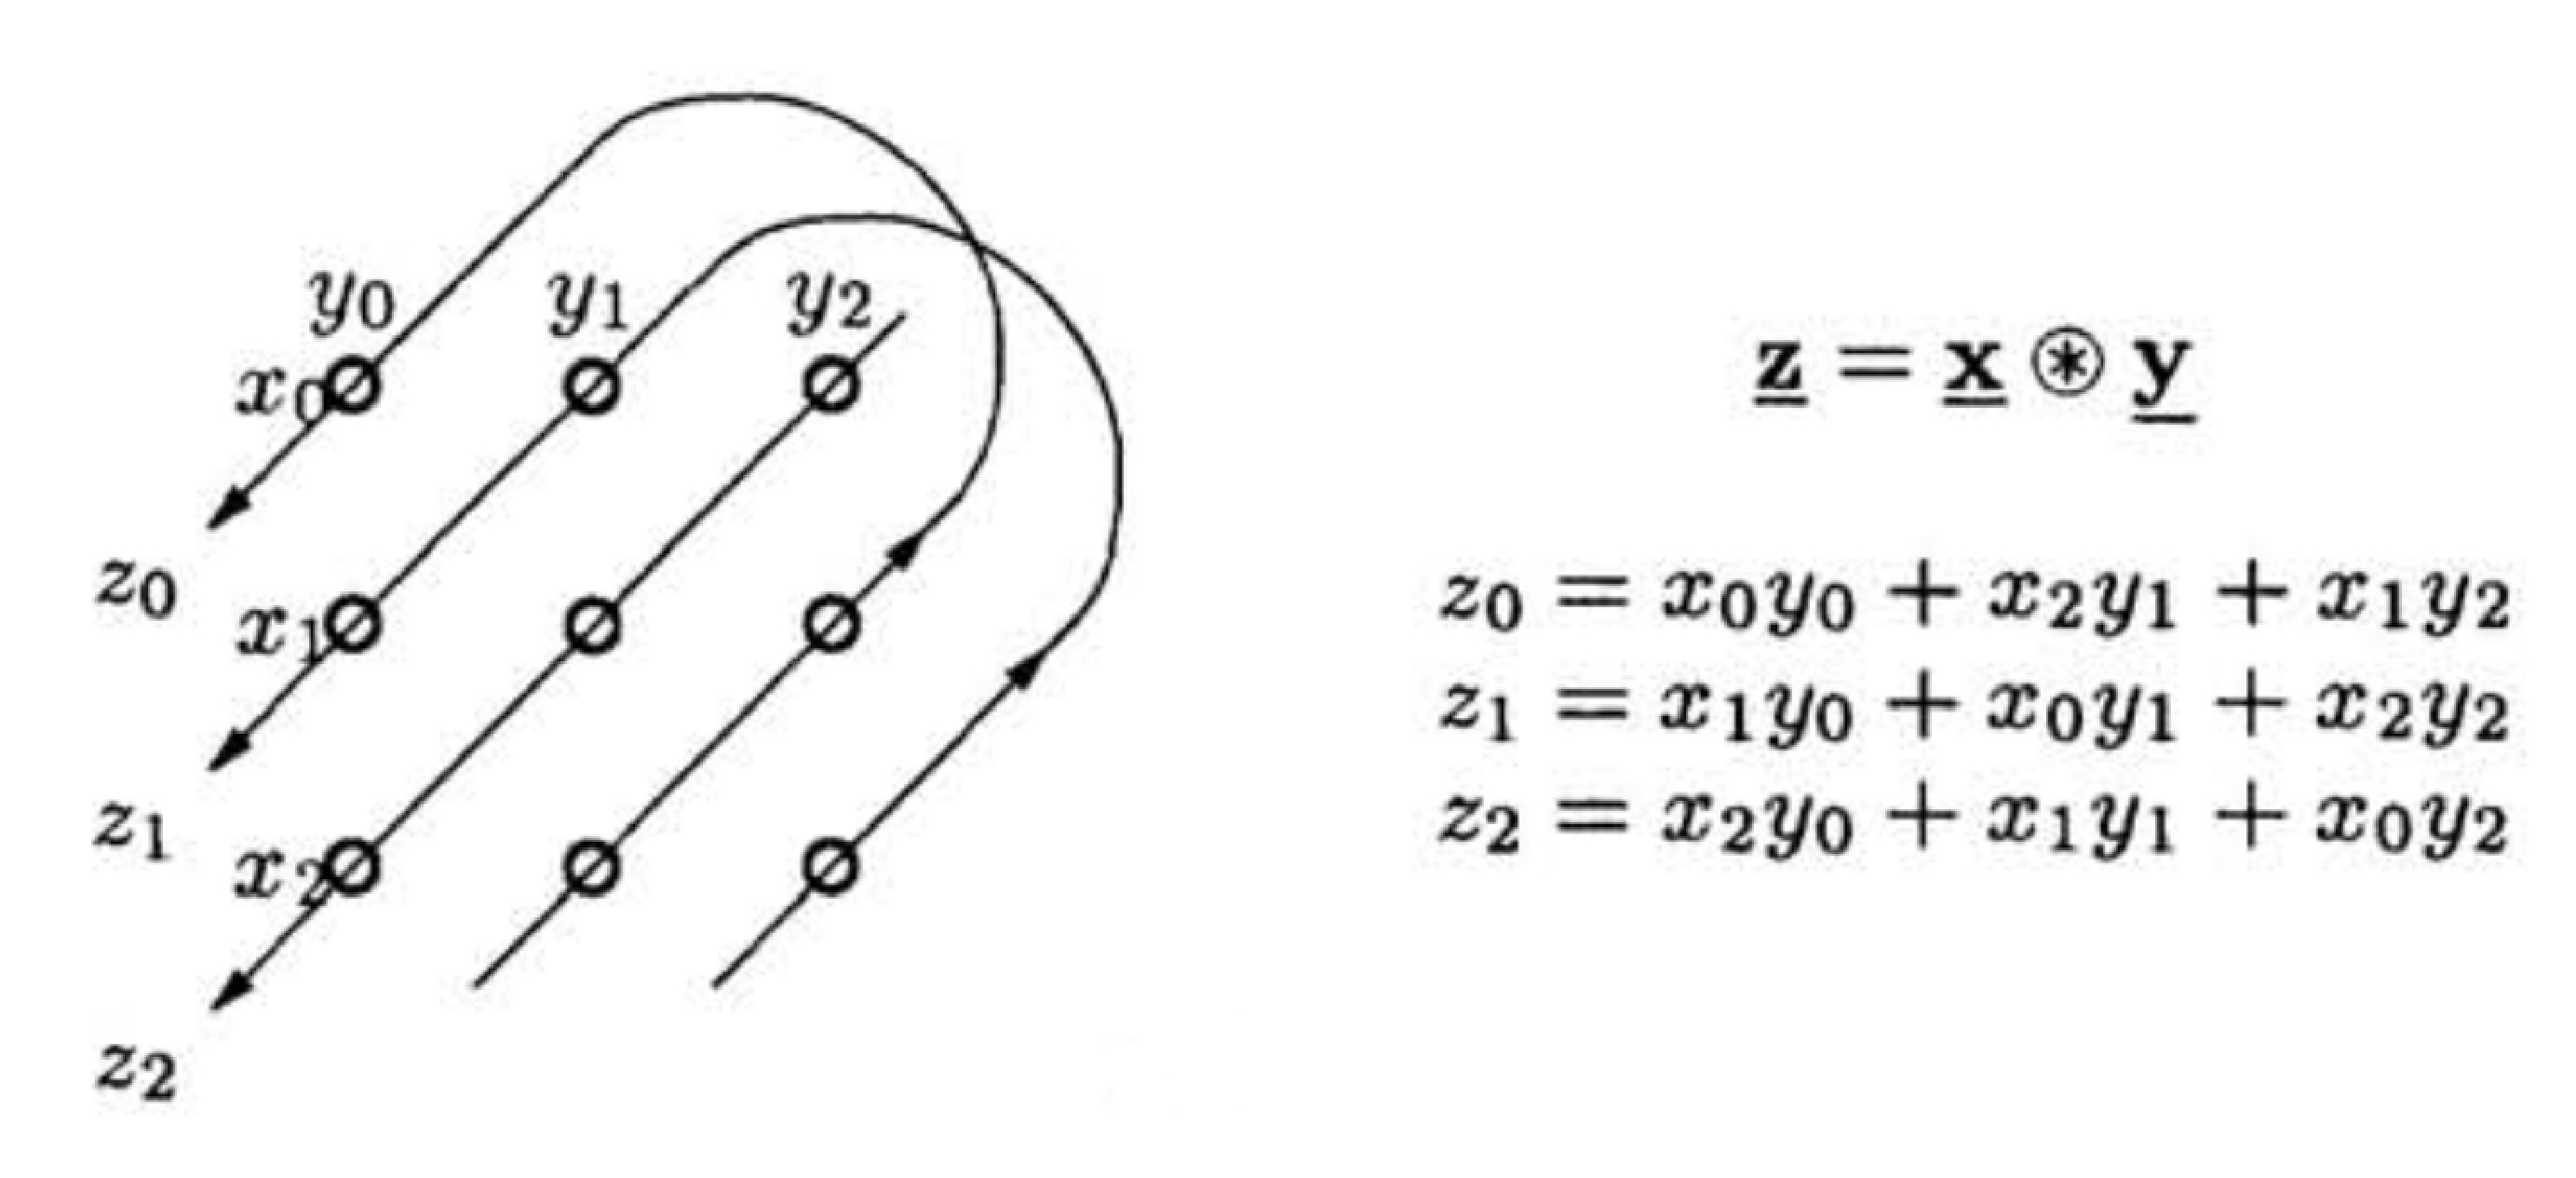
\includegraphics[width=0.85\textwidth]{imgs/circular_convolution_visualization_hor.eps}
			\caption{Visualization of circular convolution as compressed outer product for $3$-dimensional vectors. Image source \cite{Plate1994a}}
			\label{fig:circ_conv}
		\end{figure}
		The neutral element regarding circular convolution is $\pmb{1} = \left(1, 0, \cdots, 0\right)$. 
		One important property of this operation is the fact, that circular convolution can efficiently be computed using the \ac{DFT}.
		The \ac{DFT} is defined as the function
		\[
		\abb{\ac{DFT}}{\mathbb{C}^{D}}{\mathbb{C}^{D}}{x}{\left(\sum_{j=0}^{D-1} x_{j} \zeta_{D}^{-jk} \right)_{k=0}^{D-1}} \qquad \textrm{ with } \zeta_{D} = \exp\left( \frac{i 2 \pi}{D} \right).
		\]
		Similarly, the \ac{IDFT} is defined as the function 
		\[
		\abb{\ac{IDFT}}{\mathbb{C}^{D}}{\mathbb{C}^{D}}{x}{\left( \frac{1}{D} \sum_{j=0}^{D-1} x_{j} \zeta_{D}^{jk} \right)_{k=0}^{D-1}}.
		\]
		From the convolution theorem we know, that we can calculate the circular convolution of any two vectors $v, w \in V_{D}(N)$ by
		\[
		v \varoast w = \ac{IDFT}\left(\ac{DFT}(v) \odot \ac{DFT}(w) \right),
		\]
		with $\odot$ denoting element-wise multiplication in this case.
		This induces that circular convolution obeys the same rules (commutativity and associativity) as element-wise multiplication, as both operations are the same except for a change of basis. 
	\end{enumerate}
\end{ex}
As mentioned earlier, one of the most important features of (high-dimensional) \acp{VSA} is the fact that two random vectors are likely to be dissimilar.
We will derive this result in the following Theorem.
\begin{theorem}
	\label{theorem:VSA_cossim_distribution}
	Let $\left(V_{D}(N), \varoast, \oplus, \phi \right)$ a \acl{VSA}. 
	For two randomly chosen vectors $v, w \in V_{D}(N)$, the distribution of the similarity $\phi\left(v,w\right)$ is a version of the beta-distribution $\beta\left(\frac{D-1}{2},\frac{D-1}{2}\right)$ scaled and shifted to the interval $\left[-1,1\right]$ with mean $\mu=0$ and variance $\sigma^2=\frac{c^2}{D}$ up to a constant $c$. The standardized distribution trends with growing $D$ to a normal distribution.
\end{theorem}
\begin{proof}
	We will only give the proof of this Theorem for real valued \acp{VSA}, i.e. $N \subseteq \mathbb{R}$ and $\phi$ as the cosine similarity.
	Without loss of generality, we assume the vectors $v,w$ picked randomly from the unit sphere $\mathbb{S}^{D-1} = \{ v \in \mathbb{R}^{D} | \norm{v} = 1 \}$, as we can simply normalize the vectors by $\frac{v}{\norm{v}}$.
	Since binary \acp{VSA} can be associated with a euclidean sphere as well, the same result can be proven for those architectures with similar arguments (see \cite{Kanerva1988} for details).
	Due to symmetry of the unit sphere $\mathbb{S}^{D-1}$, we can furthermore - again without loss of generality - choose one vector as a unit vector, i.e. $w=\left(1, 0 , \cdots, 0\right)$.
	Thereby, the cosine similarity for $v=\left(v_{0}, \cdots, v_{D-1}\right)$ is given by $\phi\left(v,w\right) = v_{0}$
	By fixing one coordinate, we get the constraint $\sum_{i=1}^{D-1} v_{i}^{2} = 1-v_{0}^{2}$ which is equivalent to a lower dimensional sphere $\mathbb{S}^{D-2}$ with radius $\sqrt{1-v_{0}^2}$.
	Hence the cosine similarity $\phi\left(v,w\right)=:x$ is proportional to the surface of a conical frustum constructed from $\mathbb{S}^{D-2}$ with radius $\sqrt{1-x^{2}}$, slope $\frac{1}{\sqrt{1-x^{2}}}$ and some height $h$, i.e. the density function is proportional to
	\[
	f_{\phi(v,w)}(x) \propto \frac{\sqrt{1-x^{2}}^{(D-2)}}{\sqrt{1-x^{2}}} h \propto \left(1-x^{2}\right)^{\frac{D-3}{2}}.
	\]
	Substituting $x=2u-1$, we get 
	\[
	\left(1-\left(2u-1\right)^{2}\right)^{\frac{D-3}{2}} \propto \left(u-u^2\right)^{\frac{D-3}{2}} = \left(u \left(1-u\right)\right)^{\frac{D-3}{2}} = u^{\left(\frac{D-1}{2}-1\right)} \left(1-u\right)^{\left(\frac{D-1}{2}-1\right)},
	\]
	which is the density function of the beta distribution $\beta\left(\frac{D-1}{2},\frac{D-1}{2}\right)$.
	Thus, the cosine similarity is also beta distributed, but scaled and shifted to the interval $\left[-1,1\right]$ by $x=2u-1$.\\
	For $\alpha=\beta=\frac{D-1}{2}$, the mean of the beta distribution is $\tilde{\mu}=\frac{1}{2}$. Applying the substitution, we get the mean of the shifted distribution $\mu = 2\tilde{\mu }-1 = 0$.\\
	Making use of the simplification that the distribution of similarity is the same as the distribution in the first coordinate, the variance is given by the expected value of the square value of the first coordinate, i.e. $\mathbb{E}(v_{0}^{2})$.
	Since all coordinate are identically distributed, we get
	\[
	\mathbb{E}(v_{0}) = \frac{1}{D} \sum_{i=0}^{D-1} \mathbb{E}(v_{i}^2)= \frac{1}{D} \underbrace{\mathbb{E}\left(\sum_{i=0}^{D-1} v_{i}^2\right)}_{=:c^2}=\frac{c^2}{D}.
	\]
	Hence variance of the distribution of the cosine similarity is $\sigma^2=\frac{c^2}{D}$.
	In the particular case of the unit sphere $\mathbb{S}^{D-1}$, we get $c^{2}=1$ and a variance of $\sigma^2=\frac{1}{D}$.\\
	To see the convergence behaviour of the standardized distribution, we look at the logarithm of its density function %$f_{\phi(v,w)}\left(\frac{x}{\sqrt{D}}\right)$
	\begin{equation}
	\label{eq:log_dens}
	\log\left(f_{\phi(v,w)}\left(\frac{x}{\sqrt{D}}\right)\right) = \frac{D-3}{2}\log\left(1-\frac{x^2}{D}\right) + C.
	\end{equation}
	Using the Tayler series approximation of the logarithm, equation \ref{eq:log_dens} transforms to
	\begin{align*}
	\log\left(f_{\phi(v,w)}\left(\frac{x}{\sqrt{D}}\right)\right) &= \frac{D-3}{2}\left(-\frac{x^2}{D} + \frac{x^4}{4D} \pm \ldots \right) + C = -\frac{1}{2}x^2 + \frac{3}{2D}x^2 + \mathcal{O}\left(\frac{x^4}{D}\right)  + C  \\
	&\longrightarrow -\frac{1}{2}x^2 + C = \log\left(f_{\mathcal{N}}\left(x\right)\right) \textrm{ for } D \longrightarrow \infty.
	\end{align*}
	Hence, with growing $D$ the standardized distribution of the cosine similarity trends to a normal distribution. 
\end{proof} 
Theorem \ref{theorem:VSA_cossim_distribution} states, that the probability of finding two random, non-orthogonal vectors in a \ac{VSA} decreases with growing vector dimension.
Fig. \ref{fig:cosine_dist}, which shows the probability distributions of cosine similarity for different vector dimensions, illustrates this result. 
Furthermore, Theorem \ref{theorem:VSA_cossim_distribution} allows us to give a more formal definition of the term "dissimilar".
\begin{defn}
	\label{def:similar}
	Let $(V_{D}(N), \varoast, \oplus, \phi)$ be a \acrfull{VSA} of dimension $D$. We call any two vectors $v, w \in V_{D}(N)$ \emph{dissimilar}, if 
	\[ 
	\left| \phi(v,w) \right| \leq \epsilon, \textrm{ with } \epsilon:=\tfrac{3}{\sqrt{D}}.
	\]
	Analogously, we call any two vectors $v, w \in V_{D}(N)$ \emph{similar}, if	$\left| \phi(v,w) \right| > \epsilon$. 
	If furthermore 	
	\[
	1-\epsilon < \left| \phi(v,w) \right| \leq 1,
	\]
	we call $v, w \in V_{D}(N)$ \emph{highly similar}, denoted by $v \approx w$.
\end{defn}
Definition \ref{def:similar} can also be stated as follows: we consider any two vectors similar, if their similarity is higher than what we would expect from two randomly chosen vectors.
Therefore, we make use of the fact, that for growing dimension $D$, the cosine similarity follows approximately a normal distribution $\mathcal{N}\left(\mu, \sigma\right)$, with $\mu=0$ and $\sigma=\tfrac{1}{\sqrt{D}}$ and the so-called three-sigma-rule.
This rule, which follows from Chebyshev's inequality, states that the probability $\mathbb{P}\left(\mu-3\sigma \leq X \leq \mu+3\sigma \right) \geq 0.95$ for any unimodal distributed random variable $X$.
For normally distributed $X$, this probability is even approximately \SI{99.7}{\percent}.
Given Definition \ref{def:similar}, the probability of two randomly chosen vectors being similar is below \SI{0.3}{\percent}, while the actual numerical interval $\left[-3\sigma, 3\sigma\right]$ only depends on the vector dimension $D$.\\
Based on the definition of similarity, we derive criteria for "good" multiplication functions in \acp{VSA}.
\begin{defn}
	\label{def:binding}
	Let $(V_{D}(N), \varoast, \oplus, \phi)$ be a \acrfull{VSA} of dimension $D$. We call its multiplication function 
	\[\abb{\varoast}{V_{D}(N) \times V_{D}(N)}{K^{D}}{(v,w)}{\varoast(v,w) =: v\varoast w}\]
	a \emph{binding function} if 
	\begin{enumerate}
		\item for any two vectors $v, w \in V_{D}(N)$, the vector $v \varoast w$ is dissimilar to both $v$ and $w$, i.e.
		\[
		\left| \phi(v,v \varoast w) \right| \leq \epsilon \textrm{ and } \left| \phi(w,v \varoast w) \right| \leq \epsilon.
		\]
		\item for any vector $v \in V_{D}(N)$, there exists a vector $\bar{v} \in V_{D}(N)$ with $v \varoast \bar{v} \approx \mathbf{1}$. We call $\bar{v}$ a \emph{pseudo-inverse} element. 
		If furthermore $v \varoast \bar{v} = \mathbf{1}$, we call the vector $\bar{v}$ \emph{exact inverse}.
	\end{enumerate}
\end{defn}
It is worth noting, that all multiplication operations mentioned in example \ref{ex:VSAs} fulfill the criteria for binding functions as stated in Definition \ref{def:binding}. 
\begin{figure}[t!]
	\centering
	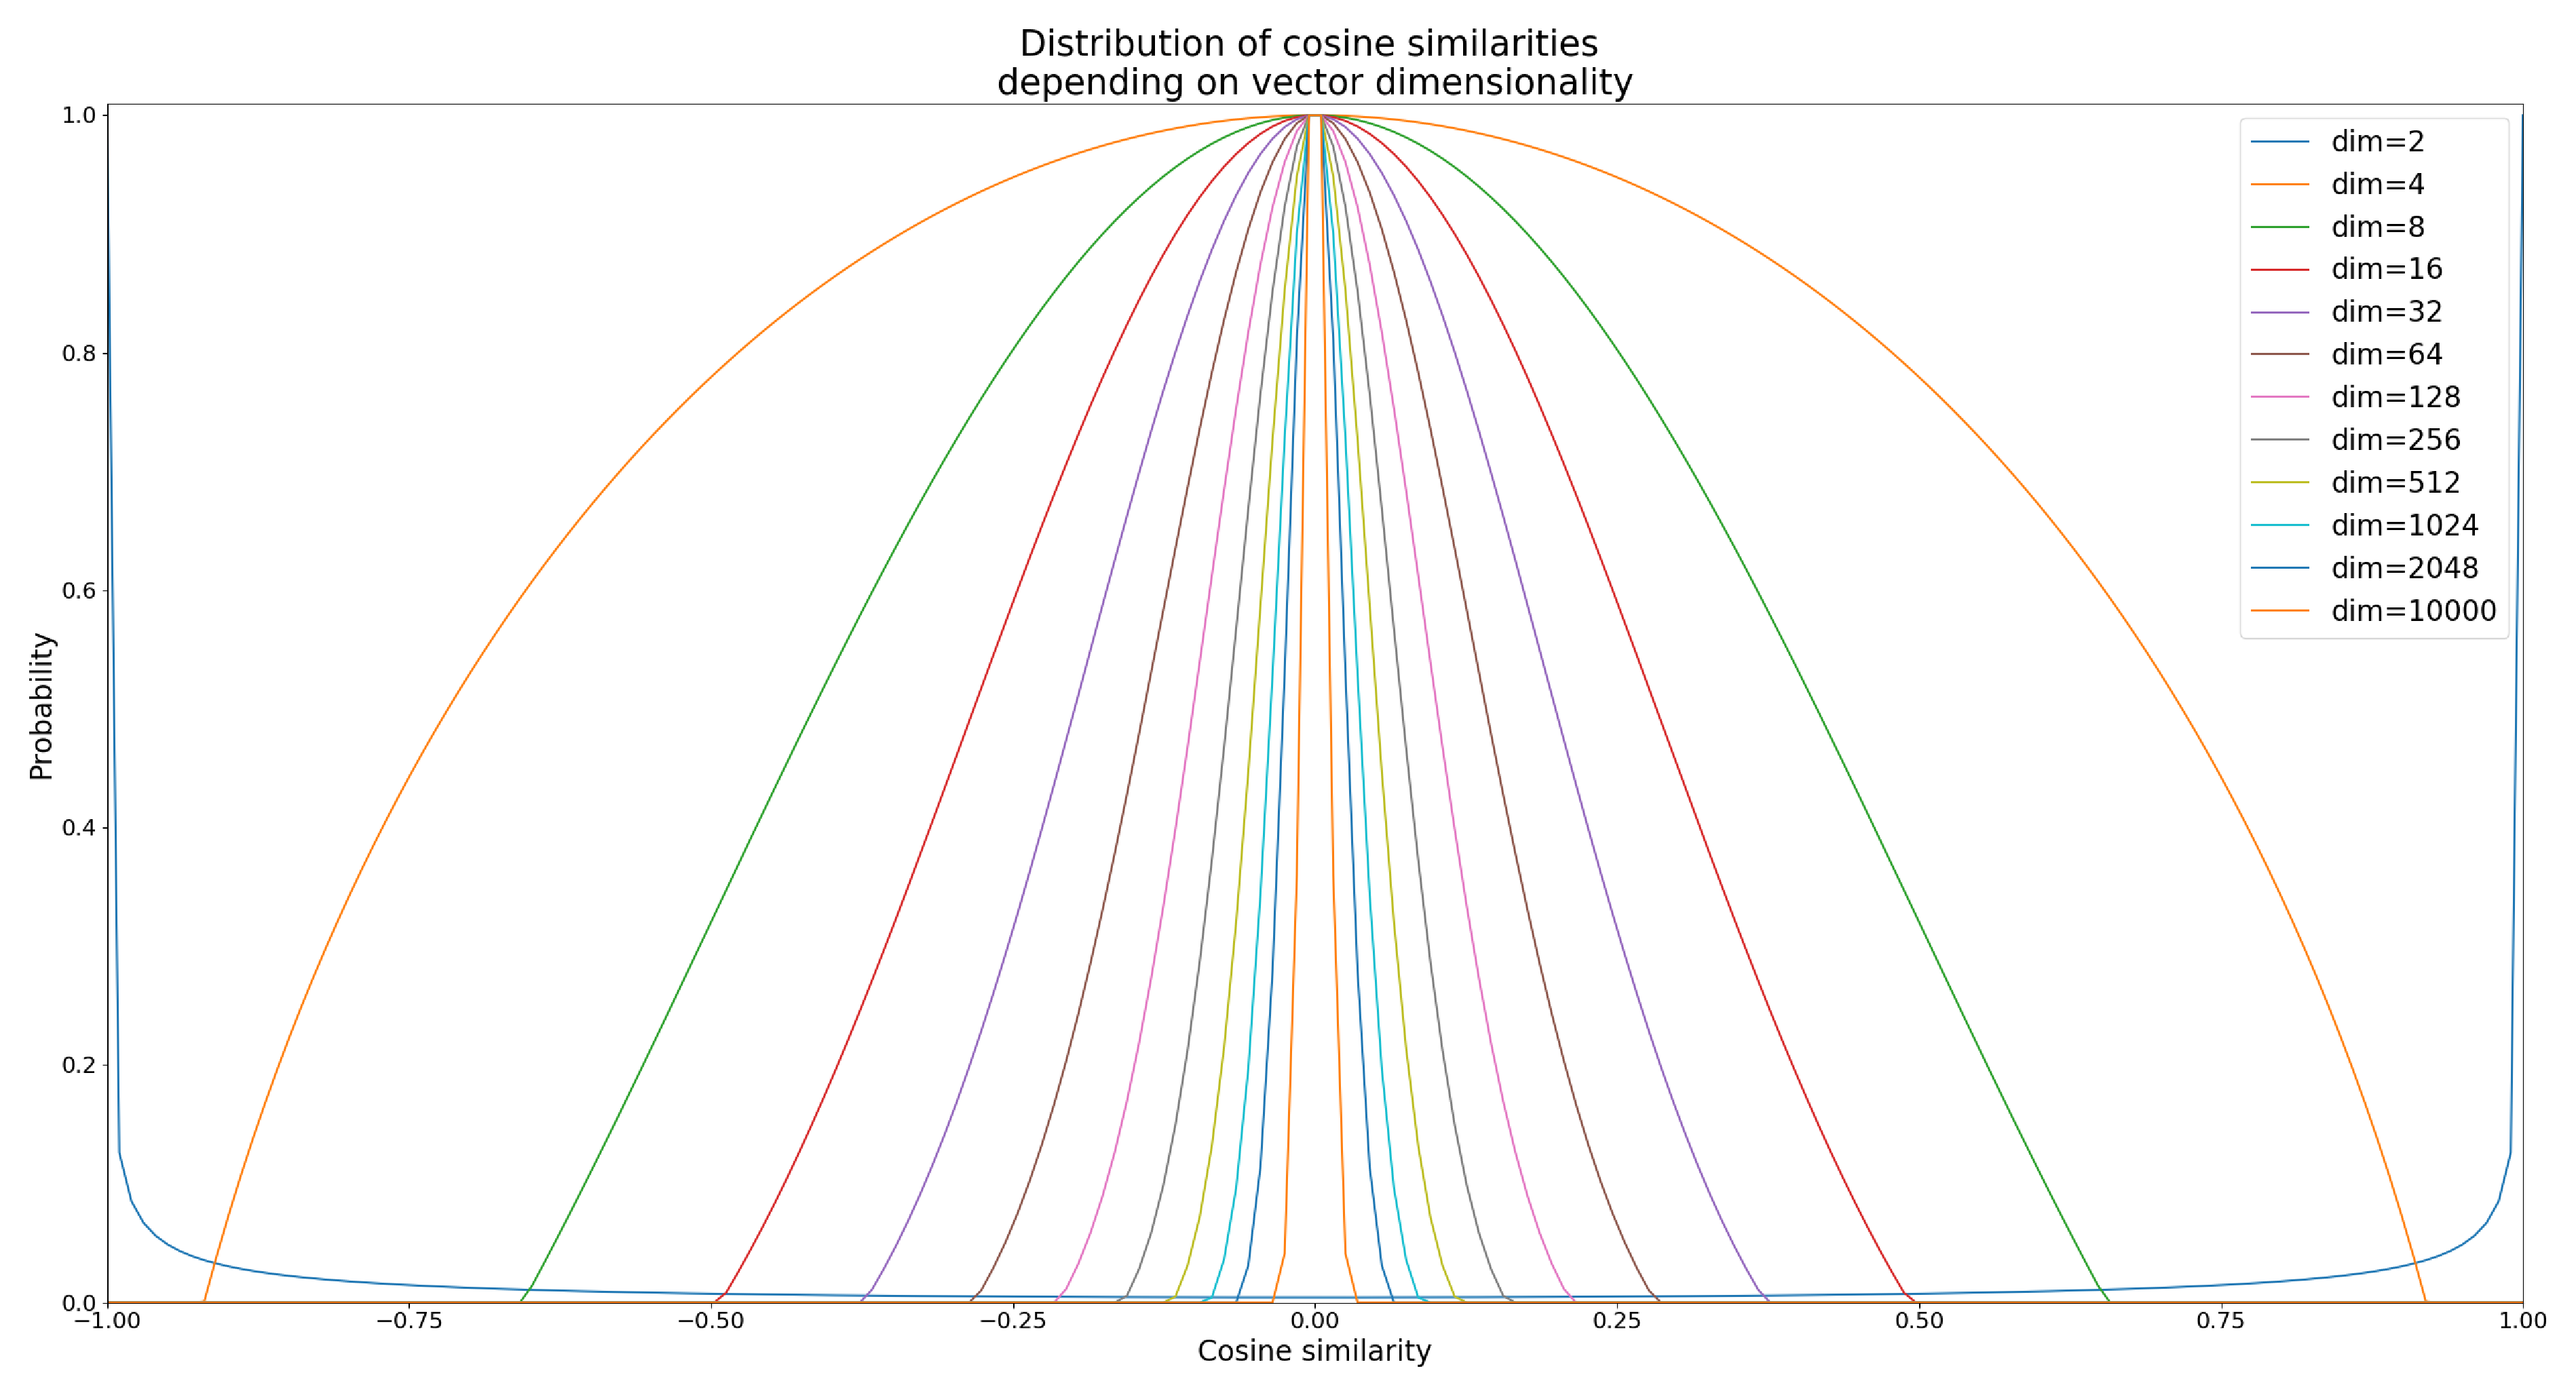
\includegraphics[width=0.85\textwidth]{imgs/distributions_cosine_sims.eps}
	\caption{Visualization of cosine similarity distributions for different vector dimensions \todo{remove figure title in python, make labels larger for better readability}}
	\label{fig:cosine_dist}
\end{figure}
The first criteria is intended to allow structured representations in \acp{VSA}.
Representations built solely upon an addition function lack a mechanism to impose structure, as the sum of vectors is similar to all summands.
For continuous \acp{VSA}, this result is straightforward due to the linearity of the dot product, but it holds true for \acp{BSC} as well.
Therefore, summing vectors only allows to encode unordered sets of entities.
The property of binding functions to map two vectors to a vector dissimilar to both inputs enables structured representations.\\
The second criteria of Definition \ref{def:binding} for binding functions is the basis to decode or recover the individual vector ingredients from structured representations.
The existence of a (pseudo-) inverse element allows the retrieval of $v,w \in V_{D}(N)$ from $v \varoast w$ by
\begin{equation}
\label{eq:retrieval}
\bar{v} \varoast \left(v \varoast w\right) = \underbrace{\bar{v} \varoast v}_{\approx \mathbf{1}} \varoast w = \tilde{w} \approx w.
\end{equation}
In case of exact inverse elements, the right hand side of equation \ref{eq:retrieval} becomes an exact equality $\tilde{w}=w$.
In most cases, however, the result $\tilde{w}$ is not exactly equal to $w$, but highly similar.
It is this inherent inexactness of most \acp{VSA} what makes them suitable candidates for cognitive modelling \cite{Eliasmith2013}.
On the other hand, it imposes a functional demand for a clean-up memory.
A clean-up memory is a mechanism, which maps noisy versions of vectors like $\tilde{w}$ to their exact counterparts, here $w$.
Therefore, we need to have a set of vectors, which represent established concepts or symbols the system has knowledge of.

\begin{defn}
\label{def:clean-up-mem}
	Let $(V_{D}(N), \varoast, \oplus, \phi)$ be a \acrfull{VSA} of dimension $D$ with binding function $\varoast$.
	We call a finite subset $\vartheta \subsetneq V_{D}(N)$ a \emph{vocabulary}.
	A function $\abbil{\gamma}{K^{D}}{\vartheta}$ is called a \emph{clean-up memory}, if 
	\begin{enumerate}
		\item for any vector $v\in K^{D}$ we have
		\[
		\phi\left(v, \gamma(v)\right) > \phi\left(v, w\right), \textrm{ for any vector } w \in \vartheta, \gamma(v) \neq w.
		\]
		\item for any two highly similar vectors $ v \neq \tilde{v} \in K^{D}, v \in \vartheta$, i.e. $\tilde{v} \approx v$, we have $\gamma(\tilde{v})=v$.
	\end{enumerate}
\end{defn}

Definition \ref{def:clean-up-mem} states, that the cleaned-up version of a vector is more similar to the original (noisy) version than any other vector in the vocabulary.

\todo{focus on \acp{HRR} and \ac{SPA} from now on add properties of (pseudo-) inverses and unitary vectors}

\subsection{Cognitive Modelling with \aclp{VSA}}
\todo{explain how modelling with VSAs works referring to neural modelling section and explain implementation in SNNs}
\chapter{Theoretical Background}
In this chapter, we briefly present the theoretical background for some frameworks and methods used throughout this thesis.


\section{\aclp{VSA}}
The term \acp{VSA} - first coined by Ross Gayler \cite{Gayler2003} - refers to a class of similar approaches for cognitive modeling making use of distributed representations.
The basic idea behind all of those approaches is to represent structure (e.g. cognitive concepts, symbols or language) in a high-dimensional vector space by mapping each entity to be represented to a (possibly random) vector.
One of the most important properties of high-dimensional vector spaces enabling this kind of representation is the fact, that two high-dimensional random vectors are likely to be dissimilar.
In the following, we will show what we mean by fuzzy terms like \emph{dissimilar} or \emph{likely} and provide more precise statements.\\
One main requirement in the context of cognitive modeling is the ability of the modeling framework to address the binding problem.
In \cite{Jackendoff2002}, Jackendoff phrases this as the problem of "combining independent bits into a single coherent percept". 
One strength of \acp{VSA} is that they offer the possibility to manipulate their entities (i.e. vectors) through algebraic operations, usually at least one \emph{addition-like} and \emph{multiplication-like} operation each.
Typically, the multiplication operation is used for binding different representations into a new vector.
This operation, depending on the vector representation, is constructed with some desirable properties in mind (see section ??\todo{insert reference}) %TODO insert reference.
A first attempt on using a multiplication operation on vectors for binding was done by Smolensky \cite{Smolensky1990} using the tensor product.
The major drawback of this approach is exploding dimensionality of the tensor product.
For finite dimensional vector spaces  $V$ and $W$ of dimensions $n$ and $m$, the tensor space $V \otimes W$ is a vector space of dimension $n\cdot m$.
As a consequence, each binding operation $v\otimes w$ for vectors $v \in V, w \in W$ would increase the dimension of the representational space, which is computationally infeasible and leads to poor scaling.
This lead researchers to define several slightly different multiplication or binding operations, depending on the underlying numerical structure.
The most prominent examples are elementwise multiplication in Gayler's \ac{MAP}-architecture \cite{Gayler1998}, the XOR-operation in Kanerva's \acp{BSC} \cite{Kanerva2000, Kanerva2009} as well as circular convolution in Plate's \acp{HRR} \cite{Plate1991, Plate1994}.

\subsection{Mathematical properties of \aclp{VSA}}
%Before we provide a formal definition for \acp{VSA}, we introduce some terms and auxiliary tools needed for later use.
%\begin{defn}
%	\label{def:metric}
%	Let $M$ be a set. A function 
%	\[
%	\abb{d}{M \times M}{\mathbb{R}}{(x,y)}{d(x,y)} 
%	\]
%	is called a \emph{metric}, if and only if for any $x, y \in M$ the following conditions hold:
%	\begin{enumerate}
%		\item $d(x,y) \geq 0$ (non-negativity)
%		\item $d(x,y) = 0 \Longleftrightarrow x = y$ (identity of indiscernibles)
%		\item $d(x,y) = d(y,x)$ (symmetry)
%		\item $d(x,z) \leq d(x,y) + d(y,z)$ (triangle inequality)
%	\end{enumerate}
%	We call the ordered pair $(M,d)$ a \emph{metric space}.
%\end{defn}
 

\begin{defn}
	\label{def:VSA}
	Let $N$ be a set of numbers and $D \in \mathbb{N}$ a natural number. 
	Furthermore, let 
	\[V_{D}(N)=\{\left(x_{0}, \cdots, x_{D-1}\right)  | x_{i} \in N\}\] 
	be the set of all $D$-tuples with entries in $N$. 
	Let
	\begin{align*}
		&\abb{\oplus}{V_{D}(N) \times V_{D}(N)}{V_{D}(N)}{(v,w)}{\oplus(v,w) =: v\oplus w}, \\
		&\abb{\varoast}{V_{D}(N) \times V_{D}(N)}{V_{D}(N)}{(v,w)}{\varoast(v,w) =: v\varoast w}
	\end{align*}
	be functions with $\oplus$ following the rules of ordinary addition - namely commutativity, associativity, existence of a neutral element and existence of inverse elements - and for any elements $u,v,w \in V_{D}(N)$
	\[u \varoast (v \oplus w) = u \varoast v \oplus u \varoast w.\]
	If there is furthermore a distinct element $\pmb{1} \in V_{D}(N)$ with 
	\[v \varoast \pmb{1} = \pmb{1} \varoast v = v\]
	for any $v \in V_{D}(N)$ and a function $\abbil{\phi}{V_{D}(N) \times V_{D}(N)}{\left[-1,1\right]}$, we call $(V_{D}(N), \varoast, \oplus, \phi)$ a \emph{\acrfull{VSA}} of dimension $D$.
	The function $\phi$ is called a \emph{measure of similarity}.
	If $N$ is a subset of the real or complex numbers, i.e. $N \subset \mathbb{R}$ or $N \subseteq \mathbb{C}$, we call any \ac{VSA} $\left(V_{D}(N), \varoast, \oplus, \phi\right)$ \emph{continuous}.
\end{defn}
Although the set $V_{D}(N)$ might not be a vector space in the strict mathematical sense (in most cases it is at least a subset of a vector space), we will refer to its elements as \emph{vectors}.
%The metric in definition \ref{def:VSA} is needed as measure of similarity between vectors. 
Before we proceed in deriving some important properties of \acp{VSA}, we present some of the most prominent examples.

\begin{ex} \aclp{VSA}
	\begin{enumerate}
		\item The first example of a \ac{VSA} is Kanerva's \acfl{BSC} \cite{Kanerva2009}. 
		He restricts the elements of his vectors to binary values, i.e. $N=\{0,1\}$
		The operations $\varoast$ and $\oplus$ in this case are the XOR-function and a thresholded sum respectively.
		With $v_{i} = \left(v_{i 0}, \cdots, v_{i D-1}\right) \in V_{D}(N)$ and  $i \in \{1, \cdots, n\}$, the operation $\oplus$ is usually defined in the following way
		\begin{align*}
		v_{1} \oplus \cdots \oplus v_{n} =: &x = \left(x_{0}, \cdots, x_{D-1}\right) \textrm{ with } \\
		&x_{j}:= \begin{cases}
		1 & \sum\limits_{i=1}^{n} v_{ij} \geq \frac{n}{2} \\
		0 & \sum\limits_{i=1}^{n} v_{ij} < \frac{n}{2}
		\end{cases}.
		\end{align*}
		This definition ensures, that the results of the addition operation $\oplus$ remain binary.
		Usually, a normalized Hamming distance 
		\[
		\phi(v,w) := 1 - \frac{2}{D} \left| \{ v_{i} \neq w_{i} | i \in \{0, \cdots, D-1\} \} \right|
		\]
		is used as a measure of similarity in this architecture.
		\acp{BSC} have some interesting properties compared to other \acp{VSA}: 
		The neutral element for both operations $\varoast$ and $\oplus$ is the vector $\pmb{0} := \left(0, \cdots, 0\right)$, while all vectors are self-inverse regarding the multiplication operation $\varoast$, i.e. $v \varoast v = \pmb{0}$ for any $v \in V_{D}(N)$.
		
		\item The first example of \ac{VSA} in continuous space is Gayler's \acrfull{MAP} architecture \cite{Gayler1998} with $N \subseteq \mathbb{R}$ and the cosine simlarity as measure of similarity 
		\[
		\phi(v,w) = \frac{v \cdot w}{\norm{v}\norm{w}}=\cos(\theta),
		\]
		with $\theta$ being the angle between the vectors $v,w \in V_{D}(N)$.
		The operations $\varoast$ and $\oplus$ are simply element-wise multiplication and addition with neutral elements $\pmb{1}=\left(1, \cdots, 1\right)$ and $\pmb{0} := \left(0, \cdots, 0\right)$ respectively.
		
		\item Another example of a \ac{VSA} in continuous space is Plate's \acfl{HRR} \cite{Plate1994, Plate1997}.
		The main difference compared to the \ac{MAP} architecture is, that Plate in general allows complex vector values, i.e. $N \subseteq \mathbb{C}$ and uses a different multiplication operation $\varoast$ - namely circular convolution.
		For any two vectors $v, w \in V_{D}(N)$, circular convolution $\varoast$ ist defined as
		\begin{align*}
		z = v \varoast w \qquad \textrm{ with } z_{j} := \sum_{k=0}^{D-1} v_{k}w_{(j-k)\Mod{D}}.
		\end{align*}
		\todo{include visualization of circular convolution}
		The neutral element regarding circular convolution is $\pmb{1} = \left(1, 0, \cdots, 0\right)$. 
		One important property of this operation is the fact, that circular convolution can efficiently be computed using the \ac{DFT}.
		The \ac{DFT} is defined as the function
		\[
		\abb{\ac{DFT}}{\mathbb{C}^{D}}{\mathbb{C}^{D}}{x}{\left(\sum_{j=0}^{D-1} x_{j} \zeta_{D}^{-jk} \right)_{k=0}^{D-1}} \qquad \textrm{ with } \zeta_{D} = \exp\left( \frac{i 2 \pi}{D} \right).
		\]
		Similarly, the \ac{IDFT} is defined as the function 
		\[
		\abb{\ac{IDFT}}{\mathbb{C}^{D}}{\mathbb{C}^{D}}{x}{\left( \frac{1}{D} \sum_{j=0}^{D-1} x_{j} \zeta_{D}^{jk} \right)_{k=0}^{D-1}}.
		\]
		From the convolution theorem we know, that we can calculate the circular convolution of any two vectors $v, w \in V_{D}(N)$ by
		\[
		v \varoast w = \ac{IDFT}\left(\ac{DFT}(v) \odot \ac{DFT}(w) \right),
		\]
		with $\odot$ denoting element-wise multiplication in this case.
		This induces that circular convolution obeys the same rules (commutativity and associativity) as element-wise multiplication, as both operations are the same except for a change of basis. 
	\end{enumerate}
\end{ex}
As mentioned earlier, one of the most important features of (high-dimensional) \acp{VSA} is the fact that two random vectors are likely to be dissimilar.
We will derive this result in the following theorem.
\begin{theorem}
	Let $\left(V_{D}(N), \varoast, \oplus, \phi \right)$ a \acl{VSA}. 
	For two randomly chosen vectors $v, w \in V_{D}(N)$, the distribution of the similarity $\phi\left(v,w\right)$ is a version of the beta-distribution $\beta\left(\frac{D-1}{2},\frac{D-1}{2}\right)$ scaled and shifted to the interval $\left[-1,1\right]$ with mean $\mu=0$ and variance $\sigma^2=\frac{c^2}{D}$ up to a constant $c$. The standardized distribution trends with growing $D$ to a normal distribution.
\end{theorem}
\begin{proof}
	We will only give the proof of this theorem for real valued \acp{VSA}, i.e. $N \subseteq \mathbb{R}$ and $\phi$ as the cosine similarity.
	Without loss of generality, we assume the vectors $v,w$ picked randomly from the unit sphere $\mathbb{S}^{D-1} = \{ v \in \mathbb{R}^{D} | \norm{v} = 1 \}$, as we can simply normalize the vectors by $\frac{v}{\norm{v}}$.
	Since binary \acp{VSA} can be associated with a euclidean sphere as well, the same result can be proven for those architectures with similar arguments (see \cite{Kanerva1988} for details).
	Due to symmetry of the unit sphere $\mathbb{S}^{D-1}$, we can furthermore - again without loss of generality - choose one vector as a unit vector, i.e. $w=\left(1, 0 , \cdots, 0\right)$.
	Thereby, the cosine similarity for $v=\left(v_{0}, \cdots, v_{D-1}\right)$ is given by $\phi\left(v,w\right) = v_{0}$
	By fixing one coordinate, we get the constraint $\sum_{i=1}^{D-1} v_{i}^{2} = 1-v_{0}^{2}$ which is equivalent to a lower dimensional sphere $\mathbb{S}^{D-2}$ with radius $\sqrt{1-v_{0}^2}$.
	Hence the cosine similarity $\phi\left(v,w\right)=:x$ is proportional to the surface of a conical frustum constructed from $\mathbb{S}^{D-2}$ with radius $\sqrt{1-x^{2}}$, slope $\frac{1}{\sqrt{1-x^{2}}}$ and some height $h$, i.e. the density function is proportional to
	\[
	f_{\phi(v,w)}(x) \propto \frac{\sqrt{1-x^{2}}^{(D-2)}}{\sqrt{1-x^{2}}} h \propto \left(1-x^{2}\right)^{\frac{D-3}{2}}.
	\]
	Substituting $x=2u-1$, we get 
	\[
	\left(1-\left(2u-1\right)^{2}\right)^{\frac{D-3}{2}} \propto \left(u-u^2\right)^{\frac{D-3}{2}} = \left(u \left(1-u\right)\right)^{\frac{D-3}{2}} = u^{\left(\frac{D-1}{2}-1\right)} \left(1-u\right)^{\left(\frac{D-1}{2}-1\right)},
	\]
	which is the density function of the beta distribution $\beta\left(\frac{D-1}{2},\frac{D-1}{2}\right)$.
	Thus, the cosine similarity is also beta distributed, but scaled and shifted to the interval $\left[-1,1\right]$ by $x=2u-1$.\\
	For $\alpha=\beta=\frac{D-1}{2}$, the mean of the beta distribution is $\tilde{\mu}=\frac{1}{2}$. Applying the substitution, we get the mean of the shifted distribution $\mu = 2\tilde{\mu }-1 = 0$.\\
	Making use of the simplification that the distribution of similarity is the same as the distribution in the first coordinate, the variance is given by the expected value of the square value of the first coordinate, i.e. $\mathbb{E}(v_{0}^{2})$.
	Since all coordinate are identically distributed, we get
	\[
	\mathbb{E}(v_{0}) = \frac{1}{D} \sum_{i=0}^{D-1} \mathbb{E}(v_{i}^2)= \frac{1}{D} \underbrace{\mathbb{E}\left(\sum_{i=0}^{D-1} v_{i}^2\right)}_{=:c^2}=\frac{c^2}{D}.
	\]
	Hence variance of the distribution of the cosine similarity is $\sigma^2=\frac{c^2}{D}$.
	In the particular case of the unit sphere $\mathbb{S}^{D-1}$, we get $c^{2}=1$ and a variance of $\sigma^2=\frac{c^2}{D}$.\\
	To see the convergence behaviour of the standardized distribution, we look at the logarithm of its density function %$f_{\phi(v,w)}\left(\frac{x}{\sqrt{D}}\right)$
	\[
	\log\left(f_{\phi(v,w)}\left(\frac{x}{\sqrt{D}}\right)\right) = \frac{D-3}{2}\log\left(1-\frac{x^2}{D}\right) + C.
	\]
	Using the Tayler series approximation of the logarithm, this transforms to
	\begin{align*}
	\log\left(f_{\phi(v,w)}\left(\frac{x}{\sqrt{D}}\right)\right) &= \frac{D-3}{2}\left(-\frac{x^2}{D} + \frac{x^4}{4D} \pm \ldots \right) + C = -\frac{1}{2}x^2 + \frac{3}{2D}x^2 + \mathcal{O}\left(\frac{x^4}{D}\right)  + C  \\
																  &\longrightarrow -\frac{1}{2}x^2 + C = \log\left(f_{\mathcal{N}}\left(x\right)\right) \textrm{ for } D \longrightarrow \infty.
	\end{align*}
	Hence, with growing $D$ the standardized distribution of the cosine similarity trends to a normal distribution.
\end{proof}
\include{chapters/vector_representations_of_automotive_scenes}
\include{chapters/driving_context_classification}
\chapter{Instantiating a cognitive model for predicting vehicle behavior}
\label{chap:behav_pred}

%\todo[inline]{check behavior prediction chapter for consistency}

Predicting future behavior and positions of other traffic participants from observations is a key problem, that needs to be solved by human drivers and automated vehicles alike to safely navigate their environment and to reach their desired goal.
Therefore, we picked behavior prediction as another task for investigating the potential of vector representations in automotive context.
In contrast to the task of classifying the current driving context presented in chapter~\ref{chap:driving_context_classification}, predicting future positions of vehicles is a regression problem, i.e., we are predicting continuous values such as spatial positions instead of discrete class labels.
However, future positions of vehicles not only depend on each vehicle's own past positions and dynamic data such as velocity and acceleration but also on the behavior of the other traffic participants in the vehicle's surroundings.
For instance, in a situation as shown in Fig.~\ref{fig:on_board_data_example}, the behavior of the target vehicle, as depicted by a solid blue and dotted orange line for past and future positions respectively, is influenced by the surrounding vehicles, as illustrated by solid and dotted gray lines for past and future positions respectively.
The target vehicle is approached from behind by a faster vehicle causing it to eventually change its lane to the right, which, for now, is still occupied by the ego-vehicle and another vehicle.
All of these external influences have an impact on the target vehicle's motion (and vice versa).
We hypothesize that structured vector representations will be able to capture these relations and mutual influence between traffic participants, which is necessary for reliable predictions.
As we aim for a model-free data representation, we avoid introducing any physical constraints or restrictions regarding our data-representation or the predicting models.
Although this allows for physically unrealistic or even impossible trajectory predictions, we want our neural network models to figure out the best predictions on their own without biasing them in any direction.
In this section, we present a representation of spatial information for multiple objects in semantic vectors of fixed length using the convolutive power introduced in Definition~\ref{def:conv_power}.
In contrast to other representations of spatial data, the dimensionality of our vectors is independent of the number of encoded entities.
We use this representation as input for simple feed-forward neural networks and more sophisticated \ac{LSTM}-based models and compare them against each other and a linear prediction model as the simplest baseline.
We conduct a thorough and detailed analysis and evaluate our  models on two different data sets, namely one proprietary data set recorded with an automated vehicle prototype and one publicly available trajectory data set.

We analyze our models with respect to the context, i.e., which model performs best depending on the current driving situation.
Furthermore, we investigate the influence of the composition of the training data on the models' performance.
Additionally, we show that by using our vector representation with a simple network architecture we can achieve results comparable to more complex models.

\section{Data and preprocessing}
\label{sec:data_preproc}

In this chapter, we use two different data sets for training and evaluation of our behavior prediction models, which we describe in more detail in subsequent sections.
We refer to those data sets as \emph{On-board} or $D_1$ (see section~\ref{subsec:onboard-dataset}), which is our main data set, and \emph{\acs{NGSIM}} or $D_2$ (see section~\ref{subsec:ngsim-dataset}), which is a publicly available data set used for reference and comparability.
In this section, we describe both data sets regarding available features, available sources of information as well as their key differences and the preprocessing procedure.

\subsection{On-board-sensors data set}
\label{subsec:onboard-dataset}

\begin{figure}[t!]
	\centering
	\includegraphics[width=\textwidth]{imgs/on_board_example_with_imgs_target.png}
    \caption{Data visualization of one driving situation example from the \emph{On-board} data set $D_1$.
        The dots in the left plot indicate the position of the vehicles and color-code the vehicle type (red=motorcycle, green=car, blue=truck, black=ego-vehicle), blue and orange lines show past and future motion of the target vehicle whereas gray lines depict the other vehicles' motion.
        The right figures show raw images of the ego-vehicle's front and rear camera with the target vehicle
    highlighted by a red rectangle.}\label{fig:on_board_data_example}
\end{figure}

This is our main data set used in this chapter.
It contains real-world data gathered using the on-board sensors of an automated vehicle prototype, which we refer to as the \emph{ego-vehicle}, during test drives mainly on highways in the area of Munich, Germany.
Therefore, we refer to this data set as the \emph{On-board} data set.
The data set contains object-lists with a variety of features obtained by fusing different sensor sources.
Apart from features about motion and behavior of the dynamic objects in the scene such as position, velocity and acceleration, which are estimated from \ac{LIDAR} sensors, there is also visual information like object type probabilities or lane information, which is acquired from additional camera sensors \parencite[see][for further information on the sensor setup]{Aeberhard2015}.
Table~\ref{tab:target_data_features} gives an overview and detailed description of the data features available in this data set, which are relevant for our models.
\begin{center}
	\begin{tabular}{|l | p{12cm}|}
		\hline
		\textbf{Data label} & \textbf{Description}\\ \hline
		Position & Lateral/Longitudinal position absolute/relative to the ego-vehicle's position estimated from range sensor readings \\ \hline
		Velocity& Lateral/Longitudinal velocity absolute/relative to the ego-vehicle's velocity estimated from range sensor readings \\ \hline
		Acceleration & Lateral/Lateral acceleration absolute/relative to the ego-vehicle's velocity estimated from range sensor readings \\ \hline
		Lane & Information about the lane relative to the ego-vehicle estimated from fused sensor reading (camera and range sensors) \\ \hline
		LaneBorderDistance & Distance to left/right border of the current lane estimated from fused sensor reading (camera and range sensors) \\ \hline
		LaneCurvature & Information about the lane curvature estimated from fused sensor reading (camera and range sensors) \\ \hline
		TypeProbability & Probability for the object being a of certain type (e.g. car or truck) estimated from camera sensors \\ \hline
	\end{tabular}
	\captionof{table}{Table depicting different features for dynamic objects within the training data}
	\label{tab:target_data_features}
\end{center}
In contrast to the data set used in chapter~\ref{chap:driving_context_classification}, the object-lists of the data set used here contain already preprocessed information as a fusion from the different available sensor sources.
This fused information about objects is available at a frequency of roughly \SI{5}{\hertz}.
The main feature of this data set is that all information (position, velocity, etc.) about vehicles other than the ego-vehicle is measured with respect to that ego-vehicle and its coordinate system.
Figure~\ref{fig:on_board_data_example} shows one example situation from this data set: the left plot depicts the already preprocessed) positional information of all vehicles detected by the ego-vehicle's on-board sensors.
The dots indicate the current position of the vehicles and color-code the vehicle type (red=motorcycle, green=car, blue=truck, black=ego-vehicle).
The blue and orange lines illustrate \SI{5}{\second} of past and future motion of the target vehicle respectively.
Solid and dashed gray lines depict the other vehicles' past and future motion respectively.
On the right-hand side, the raw images from the front and rear camera give an impression of the driving situation at hand with the target vehicle highlighted by a red box.
In total, the \emph{On-board} data set contains \num{3891} vehicles, which yield a total length of roughly \SI{28.3}{\hour} when adding up the time each individual vehicle is visible.

\subsection{\acs{NGSIM} US-101 data set}
\label{subsec:ngsim-dataset}

\begin{figure}[t!]
	\centering
	\resizebox{.95\textwidth}{!}{%
		\subfloat[\label{subfig:ngsim_highway_top_view}]{%
			\includegraphics[height=4cm]{imgs/ngsim_highway_top_view.jpg}
		}
		\subfloat[\label{subfig:ngsim_example_xy}]{%
			\includegraphics[height=4cm]{imgs/ngsim_example_xy.eps}
		}
	}
    \caption{Visualization of \emph{\ac{NGSIM}} data set:~\protect\subref{subfig:ngsim_highway_top_view} depicts the highway segment from top view perspective indicating the camera's position. Image source: \textcite{NGSIM-US101}.~\protect\subref{subfig:ngsim_example_xy} visualizes the data of one particular driving situation from the data set.}\label{fig:ngsim_dataset}
\end{figure}

The \ac{NGSIM} US-101 data set \parencite{NGSIM-US101} is a publicly available data set recorded on a segment of approximately \SI{640}{\meter} length with \num{6} lanes on the US-101 freeway in Los Angeles, California.
Although the data set was originally intended for driver behavior analysis and traffic flow models \parencite{He2017}, it has also been used to train trajectory prediction models, for instance proposed by \textcite{Altche2018, Deo2018}.
The data set was recorded using cameras observing freeway traffic from rooftops with trajectory-data being extracted later from the obtained video footage.
Figure~\ref{fig:ngsim_dataset} shows the recorded highway segment from top view perspective indicating the camera's position (Fig.~\ref{subfig:ngsim_highway_top_view}) as well as the visualization of one example driving situation (Fig.~\ref{subfig:ngsim_example_xy}).
The data set contains a total of \SI{45}{\minute} of driving data split into three \SI{15}{\minute} segments of mild, moderate and congesting traffic conditions.
Apart from positional information in lateral and longitudinal direction (in a global and local coordinate system), additional features such as instantaneous velocity, acceleration, vehicle size as well as the current lane are available for each vehicle.
The trajectory data is sampled with a frequency of \SI{10}{\hertz}.
The main difference to the \emph{On-board} data set is the fact that the \emph{\ac{NGSIM}} data set is recorded with external stationary cameras instead of a driving vehicle's on-board sensors.
Thus, there is no ego-vehicle present in the data and all information is available in absolute coordinates instead of being measured relative to one particular ego-vehicle.
In total, the \emph{\ac{NGSIM}} data set contains \num{5930} vehicles and therefore a total time of roughly \SI{91.3}{\hour} when adding up the time each individual vehicle is visible.

\subsection{Preprocessing}
\label{subsec:preproc}

In this section, we describe the preprocessing steps performed before training our models to prepare the trajectory information contained in our two data sets as input for neural networks.
Although we aim to keep these preprocessing steps as consistent as possible across both data sets, there are some mild differences, which we will point out here.
We aim to anticipate positions of dynamic objects \SI{5}{\second} into the future based on past positions \SI{5}{\second} prior to their current location for one object at a time.
As the two data sets are sampled at different frequencies, we interpolate the available data over \num{20} equidistant steps to achieve intervals of \SI{0.25}{\second} to improve consistency and comparability.
Furthermore, we translate the current position of the target vehicle, i.e., the vehicle to be predicted, to be the origin of the reference coordinate system.
That is, the current position of the target vehicle will be at position $\left(0,0\right)$ for all data samples consistently across both data sets (see Fig.~\ref{fig:on_board_data_example} and~\ref{subfig:ngsim_example_xy}).
The reason for this design choice is two-fold: on the one hand, we make samples from both data sets, which originally have different coordinate frames (global vs.\ ego-vehicle) as reference, more comparable and consistent.
On the other hand, by moving the current position of the target vehicle to the origin of the reference coordinate system of the sample, we prevent our models from treating similar trajectories differently due to positional variations.
Finally, to improve suitability of the data as input for neural networks, we divide all $x$-positions by a factor of \num{10} such that $x$-/$y$-values are scaled to a similar order of magnitude.
Since the \emph{\acs{NGSIM}} data set $D_2$ is sampled at a high frequency of \SI{10}{\hertz} and contains more data than the \emph{On-board} data set, we use only every \num{10}th data point.
Thereby, we avoid the creation of too many overlapping, and therefore too similar, data samples for the \emph{\ac{NGSIM}} data set.
Furthermore, we swapped the dimensions of the positions in the \emph{\ac{NGSIM}} data set such that for both data sets $x$- and $y$-direction correspond to longitudinal and lateral positions respectively.
For training and evaluating our models, we split both data sets into two distincts subset containing training $T_i \subset D_i$ and validation data $V_i \subset D_i$.
Those training and validation subsets contain \SI{90}{\percent} and \SI{10}{\percent} of the objects within the data sets respectively with $T_i \cap V_i = \varnothing$ to avoid testing our models on vehicles they have been trained with.

\subsection{Data set peculiarities}%
\label{subsec:data_set_peculiarities}

\begin{figure}[t]
    \centering
    \includegraphics[width=0.9\linewidth]{imgs/on_board_lane_change_example_with_imgs.png}
    \caption{Data visualization of one data sample from the \emph{On-board} data set $D_1$ containing a future lane change of the target vehicle.
        The dots in the left plot indicate the position of the vehicles and color-code the vehicle type (red=motorcycle, green=car, blue=truck, black=ego-vehicle), blue and orange lines show past and future motion of the target vehicle whereas gray lines depict the other vehicles' motion.
        The images in the top row show raw images recorded using the ego-vehicle's front and rear camera with the target vehicle highlighted by a red bounding box.}
    \label{fig:on_board_lane_change_example_with_imgs}
\end{figure}

In this section, we analyze the composition of our data sets regarding the amount of \enquote{interesting} behavior of the target vehicle.
Both, the \emph{On-board} and \emph{\ac{NGSIM}} data set consist of mainly highway driving, where we would expect mainly straight driving with the most interesting situations being the target vehicle, i.e., the vehicle whose motion we aim to predict, performing a lane change.
Hence, we are interested in the amount of situations where the target vehicle actually performs a lane change and how much more prominent normal straight driving is in both our data sets.
For the \emph{On-board} data set, we have information about the current lane as well as the distance to the lane borders estimated from the ego-vehicle's cameras available for all vehicles.
The \emph{\ac{NGSIM}} data set contains information about the current lane for each vehicle extracted from the external camera's video footage.
Thus, the selection process for the examples containing a lane change is straightforward for both data sets.
Figure~\ref{fig:on_board_lane_change_example_with_imgs} shows one data sample from the \emph{On-board} data set containing a lane change performed by the target vehicle in its future motion to be predicted.
Comparing this example to the one shown in Fig.~\ref{fig:on_board_data_example}, which shows mainly straight driving for all vehicles present in the scene, we observe that a lane change mainly influences the vehicle's motion in lateral ($y$) direction.

\begin{figure}[t]
    \centering
    \includegraphics[width=1.\linewidth]{imgs/data_set_lane_change_distribution.eps}
    \caption{Visualization of the composition of both data sets regarding lane changes of the target vehicle.}
    \label{fig:data_set_lane_change_distribution}
\end{figure}

Figure~\ref{fig:data_set_lane_change_distribution} shows the amount of situations where the target vehicle performs a lane change in comparison to the amount of situations where no such behavior occurs for both, the \emph{On-board} and \emph{\ac{NGSIM}} data set.
For the \emph{On-board} data set, in \SI{86.1}{\percent} of all data samples the target vehicle does not perform a lane change, i.e., only \SI{13.8}{\percent} of all data samples contain a lane change performed by the target vehicle.
We further distinguish between lane changes performed during the trajectory history, i.e., the past \SI{5}{\second} before the current time step (labeled as \emph{past} in Fig.~\ref{fig:data_set_lane_change_distribution}) and lane changes that are performed in the future, i.e., during the future \SI{5}{\second} from the current time step (labeled as \emph{future} in Fig.~\ref{fig:data_set_lane_change_distribution}).
We consider the lane changes in the future part of data samples to be the most interesting and challenging ones, since any model making predictions about the future trajectory needs to be able to anticipate these lane changes.
For the \emph{On-board} data set, \SI{7}{\percent} of all data samples contain a lane change in the trajectory history, while \SI{8.2}{\percent} of the samples contain a future lane change performed by the target vehicle.
In comparison to the \SI{86.1}{\percent} of data samples not containing a lane change, the amount of samples with interesting behavior other than straight driving within the data set is significantly less present.
For the \emph{\ac{NGSIM}} data set, the discrepancy between the amount of samples without the target vehicle performing a lane change and the number of samples containing a lane change is even more significant.
The percentage of samples without a target vehicle lane change is \SI{95.1}{\percent} while only \SI{4.9}{\percent} of the samples contain a lane change performed by the target vehicle at all.
The amount of samples containing a future lane change performed by the target vehicle is only \SI{2.6}{\percent} of all samples in the \emph{\ac{NGSIM}} data set.
Hence, there is a significant imbalance in both data sets between examples containing mainly straight driving by the target vehicle, namely \SI{86.1}{\percent} and \SI{95.1}{\percent} of all samples in the \emph{On-board} and \emph{\ac{NGSIM}} data set respectively, where most likely already simple prediction approaches are able to achieve reasonable results.

\subsection{Performance baselines}
\label{subsec:baselines}

\begin{figure}[th!]
	\centering
	\subfloat[Overtaking maneuvre at $t=\SI{90}{\second}$\label{subfig:overtaking1}]{%
		\includegraphics[clip,width=\columnwidth]{imgs/Vis_overtaking_maneuvre_t1.png}
	}
	\vspace{-0.3cm}
	\subfloat[Overtaking maneuvre at $t=\SI{94}{\second}$\label{subfig:overtaking2}]{%
		\includegraphics[width=\columnwidth]{imgs/Vis_overtaking_maneuvre_t2.png}
	}
	\vspace{-0.3cm}
	\subfloat[Overtaking maneuvre at $t=\SI{98}{\second}$\label{subfig:overtaking3}]{%
			\includegraphics[width=\columnwidth]{imgs/Vis_overtaking_maneuvre_t3.png}
	}
	\vspace{-0.3cm}
	\subfloat[Overtaking maneuvre at $t=\SI{100}{\second}$\label{subfig:overtaking4}]{%
			\includegraphics[width=\columnwidth]{imgs/Vis_overtaking_maneuvre_t4.png}
	}
	\caption{An example scene visualizing the data of an overtaking maneuver in a highway situation at selected time steps.}
    \label{fig:overtaking}
\end{figure}

In this section, we present and discuss the models we aim to use as performance baselines for our \ac{SPA}-based trajectory prediction approaches.
Therefore, we begin with an example:
Figure~\ref{fig:overtaking} shows an overtaking maneuver in a highway situation from the \emph{On-board} data set at four different selected time steps.
The ego-vehicle is overtaken by another car, the target vehicle to be predicted, approaching from behind.
During that overtaking maneuver, the ego-vehicle itself performs a lane change from the middle to the most right of the three lanes.
Figures~\ref{subfig:overtaking1}--~\ref{subfig:overtaking4} show different times of the situation.
Solid lines indicate previous positions whereas dashed lines indicate future positions or predictions.
The solid blue line depicts the past motion of the target vehicle overtaking the ego-vehicle, while solid gray lines visualize the past positions of other vehicles in the scene.
The dashed green line illustrates predictions from a simple linear model based on a constant velocity assumption.
This example illustrates the general trend we observe for both data sets used in this chapter that already simple linear prediction models achieve solid prediction accuracy, especially in $x$-direction.
This makes sense as both data sets almost exclusively contain highway driving situations, which in turn consists of significantly more straight driving and rather rare lane-change maneuvers as analyzed in section~\ref{subsec:data_set_peculiarities}.
For straight driving, linear prediction based on a constant velocity assumption is already a solid prediction approach, especially if all dynamic information (position, velocity etc.) is given relative to an already moving ego-vehicle like with the \emph{On-board} data set $D_1$.
Hence, we use these linear prediction models based on a constant velocity assumption as the simplest baseline models to compare our neural models using our distributed vector representations as input.

The analysis of related research on trajectory prediction in automotive context given in section~\ref{subsec:trajectory_prediction} suggests, that the most successful current state-of-the-art approaches rely mainly on \ac{LSTM}-based neural network architectures.
They are typically combined with other neural networks such as convolutional layers or classification networks \parencite{Deo2018a} to improve model performance.
In this chapter, we use \ac{LSTM}-based models as well as simpler feed-forward neural networks to predict trajectories based on our semantic vector representation of the current driving situation.
Hence, we use the same models just employing a different encoding (see section~\ref{subsec:scene_representation_in_vectors} for further details on the reference encoding schemes) of the input data avoiding further complexity of additional networks or layers to make the models as comparable as possible.

\section{Representation and models}
\label{sec:repr_models}

In this section, we describe the models we use for the behavior prediction task.
The input data for our models are sequences of positional data either as raw numerical values or in the form of semantic vectors as described in section~\ref{subsec:scene_representation_in_vectors}.
\ac{LSTM}-based neural network architectures have proven to be powerful tools for sequential data analysis and are widely used for behavior, or more generally, motion prediction.
We also investigate much simpler feed-forward neural networks constructed using the principles of the \acf{NEF} (c.f.\ section~\ref{sec:neural_eng}) to evaluate the performance gains achieved by the more complex \ac{LSTM} models.
To encode spatial information of driving situations in sequences of semantic vectors of fixed length, we employ the convolutive vector power introduced in Definition~\ref{def:conv_power} and analyzed in sections~\ref{subsec:different_vector_representations_for_numerical_values} and~\ref{subsec:capacity_analysis_limitations_to_vector_representations}.
For reference, we also describe a simpler vector representation employing the scalar multiplication encoding of numerical values also shown in section~\ref{subsec:different_vector_representations_for_numerical_values} as well as a raw numerical representation encoding only the positional information of the target vehicle.  
Furthermore, we describe the architecture of the learning models used for behavior prediction from that input data.
Importantly, here we use our models to predict one particular target vehicle at a time instead of trying to jointly predict the progress of the entire scene.
To achieve a forecast of the development of all vehicles in the scene, we would deploy several instantiations of the same network.
Using this approach, we only have to train one model while we can use each detected vehicle as training example, which significantly increases the amount of training data. 

\subsection{Scene representation in vectors}%
\label{subsec:scene_representation_in_vectors}

We use three different encoding schemes of the positional input data in this chapter.
Our main encoding scheme is the semantic vector representation as depicted in the following section making use of the convolutive vector power to encode numerical values (see also section~\ref{subsec:different_vector_representations_for_numerical_values}).
We also apply two other encoding schemes using the scalar multiplication encoding of numerical values in vectors (see also~\ref{subsec:different_vector_representations_for_numerical_values} as well as simply using the raw numerical values of the input data.

\subsubsection{Convolutive power representation}%
\label{ssubsec:convolutive_power_representation}

\begin{figure}[t!]
  \centering
  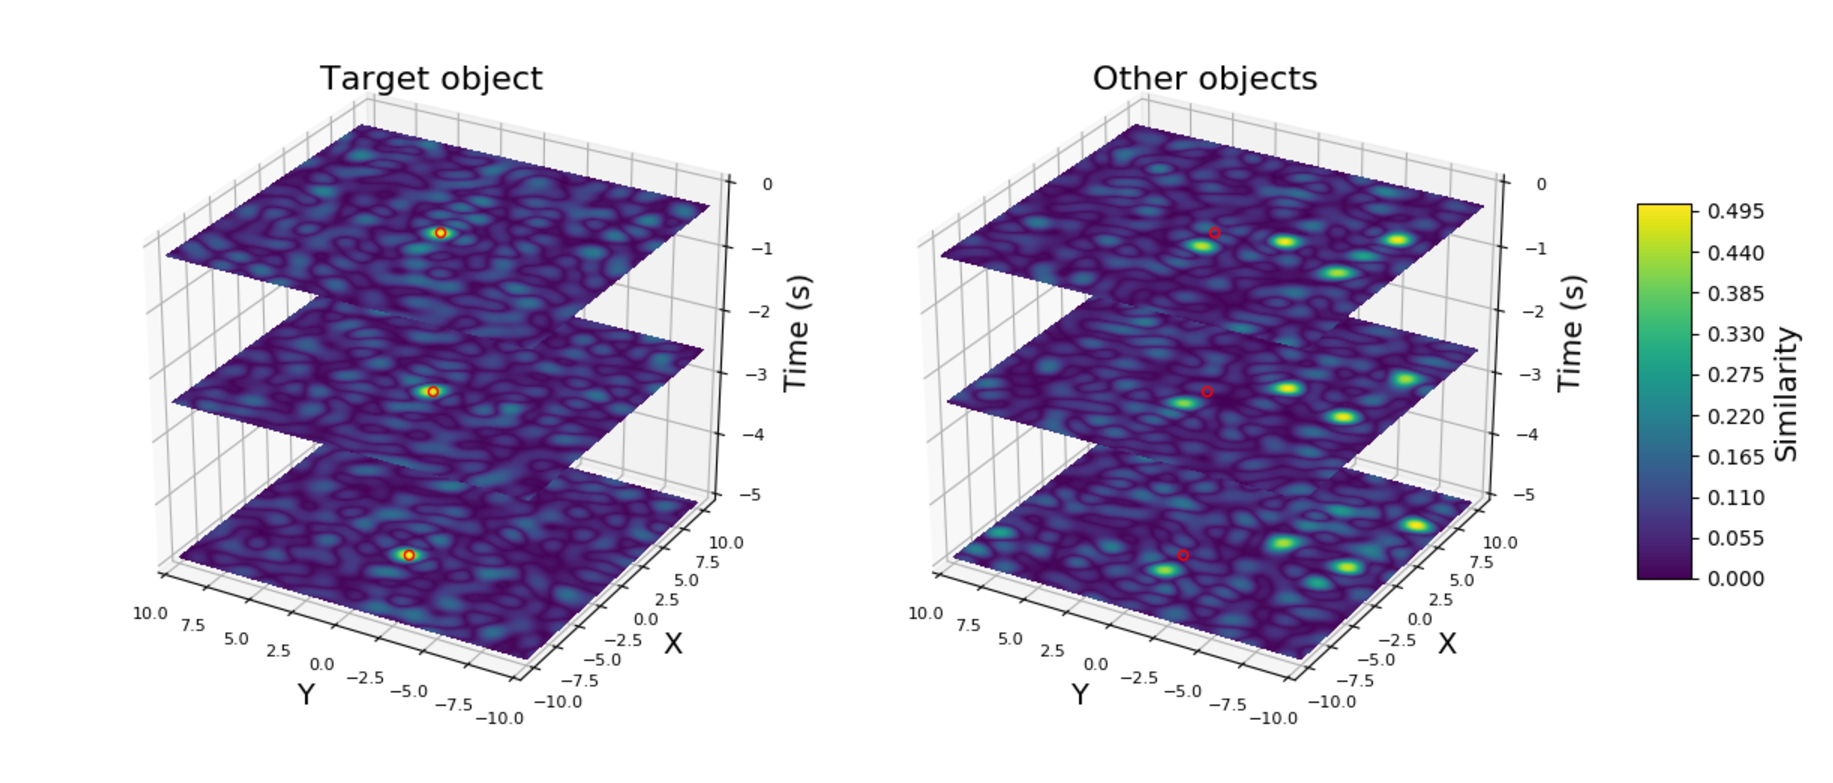
\includegraphics[width=0.95\textwidth]{imgs/spa_power_representation_in_time_viridis.eps}
  \caption{Visualization of the convolutive vector-power representation of one particular driving situation over time at selected time-steps as a heat map of similarity values for \num{512}-dimensional vectors. 
  The red circles indicate the measured position of the target vehicle.}
  \label{fig:spa_power}
\end{figure}

In this section, we investigate the expressive power of encoding the spatial positions of multiple vehicles using the convolutive vector-power introduced in Definition~\ref{def:conv_power}.
Given the results of section~\ref{subsec:the_influence_of_varying_vocabularies} that the impact of similarity structures in rather small vocabularies is neglectable, we create a random vocabulary $V$ of atomic vectors here.
We assign a random real-valued vector from the unit sphere to each category of dynamic objects (e.g.\ car, motorcycle, truck) as well as random unitary vectors (c.f.\ Definition~\ref{def:unitary_vec}) $\mathbf{X}$ and $\mathbf{Y}$ to encode the units of spatial positions in vectors.
We use unitary vectors $\mathbf{X}$ and $\mathbf{Y}$ since they have unit length and are closed under convolutive exponentiation as shown in Lemma~\ref{lemma:unitary_vec}.
Therefore, by encoding spatial positions with powers of unitary vectors, we avoid exploding lengths of our final scene vectors, which would lead to additional noise and unwanted behavior when using them as input for neural networks.
Furthermore, we use additional random ID-vectors $\mathbf{TARGET}$ and $\mathbf{EGO}$ representing the target object to be predicted and, if applicable, the ego-vehicle.
Given a situation as shown in Fig.~\ref{fig:on_board_data_example} with a sequence of prior positions $(x_{t}, y_{t})$ for the target vehicle at time step $t \in \left\{t_{0}, \ldots, t_{N} \right\}$ and equivalent sequences $(x_{obj,t}, y_{obj,t})$ for other traffic participants, we encapsulate this information in a scene vector

\begin{equation}
	\label{eq:conv_power_enc}
  \mathbf{S}_{t} = \underbrace{\mathbf{TARGET}\varoast \mathbf{TYPE}_{target} \varoast \mathbf{X}^{x_{t}} \varoast \mathbf{Y}^{y_{t}}}_{\textrm{target-vehicle}} \oplus \underbrace{\sum_{obj} \mathbf{TYPE}_{obj} \varoast \mathbf{X}^{x_{obj,t}} \varoast \mathbf{Y}^{y_{obj,t}}}_{\textrm{other objects}},
\end{equation}

This yields a sequence of semantic scene vectors $\mathbf{S}_{t}$ for $t \in \left\{t_{0}, \ldots, t_{N} \right\}$ encoding the past spatial development of objects in the current driving situation.
An alternative option could be to simply sum up the vectors at each past time step to encode the complete motion history within a single vector.
However, given the results regarding the capacity of the convolutive power encoding shown in section~\ref{subsec:capacity_analysis_limitations_to_vector_representations}, we decided for a sequence of individual vectors instead, which is also a more suitable input to neural networks employing \ac{LSTM} units.
Figure~\ref{fig:spa_power} depicts the aforementioned scene vector representation: the left plots show similarities (depicted as heat map) between the vector $\mathbf{S}_{t}$ encoding the scene from Fig.~\ref{fig:on_board_data_example} and the vectors $ \mathbf{v}_{i}=\mathbf{TARGET}\varoast \mathbf{TYPE}_{target} \varoast \mathbf{X}^{\bar{x}_{i}} \varoast \mathbf{Y}^{\bar{y}_{i}}$ for a sequence of discrete position samples ${\bar{x}_{i}, \bar{y}_{i}}$.
Similarly, the right plots show similarities between $\mathbf{S}_{t}$ and $\mathbf{CAR} \varoast \mathbf{X}^{\bar{x}_{i}} \varoast \mathbf{Y}^{\bar{y}_{i}}$ visualizing all other objects in the scene of type \emph{car}.
Importantly, each vector in the sequence $ \mathbf{S}_{t}$, i.e., each plane in the sequence of heat maps shown in Fig.~\ref{fig:spa_power} is a spatial encoding vector of the type depicted Fig.~\ref{fig:spa_power_encoding}
Hence, we can encode spatial information of several different objects in a sequence of semantic vectors and reliably decode it back out.
This allows us to encode automotive scenes with varying number of dynamic objects in a vector representation of fixed dimension.
Note that by using this vector representation as input data for a neural network (or any other predictor), we predict the future position of one other traffic participant at a time.
The indication vector $\mathbf{TARGET}$ bound to the target vehicle, i.e., the object we want the model to predict, indicates the network the current focus.
To predict all objects present in a scene during deployment, multiple instantiations of the same network can be used.
Thereby, the amount of training data generated per file increases with the number of objects while we only need to train one network.

To avoid accumulation of noise in the vectors (cf.\ section~\ref{subsec:capacity_analysis_limitations_to_vector_representations}) while focusing on the vehicles most relevant for prediction, we only use objects closer than \SI{40}{\meter} to the target vehicle in the \emph{On-board} data set.
For the \emph{\ac{NGSIM}} data set $D_2$, we additionally include only objects on the same lane as the target vehicle and on adjacent lanes.
Thereby, we aim for consistency across both data sets and we keep the input data as comparable as possible to what a driving vehicle could be able to detect using its on-board sensors.

For the \emph{On-board} data set $D_1$, we use two different variants of this representation, which differ in that the ego-vehicle's position is used or excluded in the \emph{other objects} part of Equation~\eqref{eq:conv_power_enc}, yielding two sequences $(\mathbf{S}_{t}^{ego})_{t_0}^{t_N}$ and $(\mathbf{S}_{t})_{t_0}^{t_N}$.
We used \acs{Nengo}'s \ac{SPA} package for implementation and therefore refer to these two encoding schemes $(\mathbf{S}_{t})_{t_0}^{t_N}$ and $(\mathbf{S}_{t}^{ego})_{t_0}^{t_N}$ as \emph{\ac{SPA}-power} and \emph{\ac{SPA}-power-with-ego} respectively.
As the \emph{\ac{NGSIM}} data set $D_2$ does not contain an ego-vehicle, we only investigate the \emph{\ac{SPA}-power} encoding scheme there.

\subsubsection{Reference encoding schemes}%
\label{ssubsec:reference_encoding_schemes}

For a simple reference vector-representation, we employ the scalar multiplication encoding for numerical values shown in section~\ref{subsec:different_vector_representations_for_numerical_values}.
Therefore, we add the positional vectors $\mathbf{X}$ and $\mathbf{Y}$ scaled with the target vehicle's prior positions $(x_{t}, y_{t})$ at each time step $t$, yielding the sequence $\tilde{\mathbf{S}}_{t} =  x_{t} \cdot \mathbf{X} + y_{t}\cdot \mathbf{Y}$.
We refer to this simpler encoding scheme based on the scalar multiplication encoding as \emph{\ac{SPA}-simple}.
Finally, we also use plain numerical position values $p_t = (x_{t}, y_{t})$ as another reference encoding scheme of the input data to our learning models, which we refer to as \emph{numerical}.
Importantly, only the \emph{\ac{SPA}-power} representation variants $(\mathbf{S}_{t})_{t_0}^{t_N}$ and $(\mathbf{S}_{t}^{ego})_{t_0}^{t_N}$ contain positional information about vehicles other than the target.

\subsection{\acs{LSTM}-based prediction models}%
\label{subsec:lstm_based_prediction_models}

\begin{figure}[t!]
  \centering
  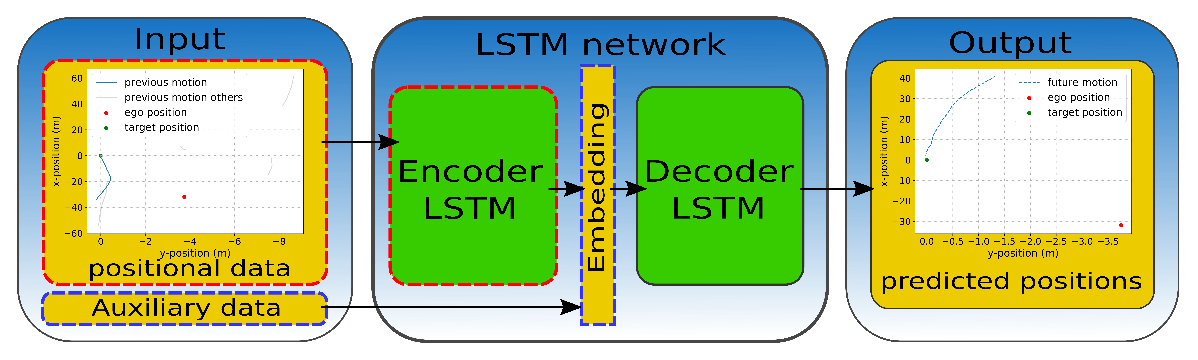
\includegraphics[width=0.95\textwidth]{imgs/lstm_arch.eps}
  \caption{Visualization of our \ac{LSTM}-based learning architecture. Modules that change with varying encoding scheme of the input data are highlighted through dashed red borders whereas parts that change when varying the data set are highlighted through dashed blue borders.}\label{fig:lstm_arch}
\end{figure}

In this section, we use a \acf{LSTM} \parencite{Hochreiter1997} network-architecture for the prediction of vehicle positions.
Our network consists of one \ac{LSTM} encoder and decoder cell for sequence to sequence prediction, which means that the input and the final result of our model is sequential data.
The encoder \ac{LSTM} takes positional data for $20$ past, equidistant time frames as input.
That is, the input data is a sequence of \num{20} items of either positions of the target vehicle or a sequence of high-dimensional vectors encoding this positional data.
The resulting embedding vector encodes the history of the input data over those time frames.
This embedding vector is concatenated with additional auxiliary information to aid the model when predicting the future trajectory of the target vehicle.
This auxiliary data is information, that is available to the system when the prediction is to happen, i.e., sensory data available at prediction time or future data about the ego-vehicle such as its own planned trajectory (see section~\ref{subsec:evaluation_of_the_lstm_based_prediction_models} for further details on this auxiliary data).
Finally, the embedding vector is used as input for the decoder \ac{LSTM} to predict future vehicle positions.
The output of each model is a sequence of \num{20} positions of the target vehicle predicted over a certain temporal horizon into the future.
We use the same network architecture for all encoding schemes of the input data and for both data sets.
However, the dimensionality of the input and the information used as auxiliary information to enrich the embedding vector vary over different encoding schemes and data sets respectively.
Figure~\ref{fig:lstm_arch} visualizes the architecture of our \ac{LSTM} models indicating modules that change when varying the encoding scheme by a dashed red border whereas parts that change with the data set are highlighted through a dashed blue border.

\subsection{Simple feed-forward \acs{NEF}-based prediction models}%
\label{subsec:simple_feed_forward_nef_based_prediction_models}

As an alternative to the \ac{LSTM}-models, we also considered a much simpler single-hidden-layer network defined using the \acf{NEF} \parencite{Eliasmith2003}.
While this is usually used for constructing large-scale biologically realistic neuron models \parencite{Eliasmith2012}, the \ac{NEF} software toolkit \acs{Nengo} \parencite{Bekolay2014} also allows for traditional feed-forward artificial neural networks using either spiking or non-spiking neurons.
For these \ac{NEF} networks, we use a single hidden layer, with randomly generated (and fixed) input weights, and use least-squares optimization to compute the output weights.
We employ the principles of the \ac{NEF} as shown in section~\ref{sec:neural_eng} to instantiate and train these models.
As with any traditional network, we can have any number of input, output, and hidden neurons, all following this same process.
The goal here is to provide a simple baseline for comparison to the \ac{LSTM} networks, to see what (if any) performance gain is produced by the more complex network approach.
However, these simpler networks are unable to process sequential data in the same way as the \ac{LSTM} models.
Therefore, we will have to slightly adapt our data, especially the semantic vector sequences, to make it suitable as input for the feed-forward networks.

\subsection{Excursion on unsupervised anomaly detection}%
\label{subsec:excursion_on_unsupervised_anomaly_detection}

In this section, we take a brief detour on anomaly detection.
We are further interested in the information encapsulated within our semantic vector representation and if it can be used to detect potentially dangerous driving situations from just the vector representation.
\acp{VSA} in general already have an intrinsic mechanism of comparing vectors with one another through the measure of similarity $\phi$.
However, it is not clear if simply comparing vectors in terms of similarity to, for instance, the mean pairwise-similarity of all known vectors, or a subset of vectors considered \enquote{normal}, will differentiate outliers from the \enquote{normal data}.
A-priori, it might not even be clear what vectors belong to the baseline set of normal data or how to define vectors to be considered as inliers.
One option could be to manually define metrics such as the number of vehicles in the scene or a threshold for the distance between the vehicles to detect crowded and potentially dangerous situations.
However, such an approach suffers from the typical issues of manual engineering such as biases introduced by the human designer as well as poor scaling.
Therefore, we employ an unsupervised learning approach based on fully-connected autoencoder neural networks similar to the one proposed in \textcite{Chen2017}.
We train an autoencoder neural network on the latest vector in the sequence $(\mathbf{S}_{t})_{t_0}^{t_N}$ of our scene vectors based on the convolutive vector-power representation in unsupervised fashion.
Thereby, the network is trained to reconstruct, i.e., generate replicates of, the data it is given.
Once the network is trained on a sufficiently large data set, we can calculate the element-wise error between the original vector $ \mathbf{v} = \left(v_{0}, \ldots, v_{D-1}\right)$ and the replicate vector $ \tilde{\mathbf{v}} = \left(\tilde{v}_{0}, \ldots, \tilde{v}_{D-1}\right)$ generated by the neural network autoencoder, i.e.,
\begin{equation}
\label{eq:anom_error}
\epsilon_{ \mathbf{v}} = \sqrt{ \frac{1}{D} \sum\limits_{i=0}^{D-1} \left(v_{i} - \tilde{v}_{i}\right)^{2}}.
\end{equation}
Vectors exceeding a certain threshold $c$ for this reconstruction error, i.e., $\epsilon_{ \mathbf{v}} > c$ will be considered as outliers or anomalies.
The threshold $c$ is generated from the percentage of examples we expect to be anomalies within the data set, which is typically chosen in the range of \SIrange{5}{15}{\percent}.

\section{Experiments and results}
\label{sec:experiments}

In this section, we describe the training process and parameters of all our models and give a detailed analysis and evaluation of the results achieved.
The \ac{LSTM} models are implemented in Tensorflow \parencite{Abadi2016} whereas the \ac{NEF} models are implemented using the \acs{Nengo} software suite \parencite{Bekolay2014}.
We use the \ac{RMSE} as our main metric for evaluation purposes.
In contrast to earlier work, we inspect the \ac{RMSE} for lateral and longitudinal directions separately to give more detailed insights into the models' behavior.
Calculating the \ac{RMSE} of the Euclidean distance would absorb the influence of the lateral \ac{RMSE} since it is an order of magnitude smaller than the longitudinal \ac{RMSE}, while we consider both directions to be at least equally important.
The lateral \ac{RMSE} is even more informative regarding the models' performance on, for instance, lane change maneuvers.
For all evaluations in this section, we refer to the longitudinal and lateral direction as $x$- and $y$-direction respectively.
Furthermore, we investigate where the models show their best performance looking for correlations between prediction accuracy and specific driving situations.

For both model types, we follow the same order of analyzing steps: firstly, we perform an investigation of the model's hyperparameters to find the best possible configuration for each model.
Secondly, we describe the process of training each model with all peculiarities corresponding to the data used or the training process itself.
Finally, we evaluate the trained models and compare their performance.
For the hyperparameter analysis, we conduct a thorough investigation on both our network architectures using only numerical input data for simplicity and to keep the time needed for training limited.
Systematically, we only analyze one parameter at a time and fix the best value for that parameter for the subsequent analysis of other parameters.
However, we also inspect certain parameter pairs jointly if there are correlations or mutual influences between the parameters to be expected.
All hyperparameter analyses in this section on both model types are performed on the \emph{On-board} data set $D1$.
If not declared otherwise, all figures show the performance of the investigated models on the validation part $V_1 \subset D_1$ of the \emph{On-board} data set.
The training process however is intended to be kept as coherent as possible between the data sets and differences having an impact on the training process will be highlighted where necessary.
Finally, we evaluate both model types' performance on both available data sets and, especially for the \ac{LSTM}-based models, we give a thorough analysis on which model performs best depending on the current driving context.
Thereby, we will identify strengths and weaknesses of each particular model.

\begin{center}
    \resizebox{\textwidth}{!}{%
        \begin{tabular}{cccccccc}
            \toprule
            \thead{Short name} & \thead{Input} & \thead{Position \\ encoding} & \thead{Network \\ architecture} & \thead{Training} & \thead{Number of \\ Units/Neurons} & \thead{Data set}\\ 
            \midrule
            linear & \makecell{current position \\ and velocity} & - & Linear regression & - & - & both \\ 
            \midrule
            LSTM numerical & sequence of positions & - & \makecell{\acs{LSTM} with one \\ encoder/decoder cell each} & \makecell{Offline, \\ backpropagation} & \makecell{\num{150} units \\ per cell} & both \\ \midrule
            LSTM \acs{SPA} \num{1} & semantic vector sequence & convolutive power & \makecell{\acs{LSTM} with one \\ encoder/decoder cell each} & \makecell{Offline, \\ backpropagation} & \makecell{\num{150} units \\ per cell} &both \\ 
            \midrule
            LSTM \acs{SPA} \num{2} & semantic vector sequence & scalar multiplication & \makecell{\acs{LSTM} with one \\ encoder/decoder cell each} & \makecell{Offline, \\ backpropagation} & \makecell{\num{150} units\\  per cell} &both \\ 
            \midrule
            LSTM \acs{SPA} \num{3} & semantic vector sequence & \makecell{convolutive power \\ incl.\ ego-vehicle} & \makecell{\acs{LSTM} with one \\ encoder/decoder cell each} & \makecell{Offline, \\ backpropagation} & \makecell{\num{150} units \\ per cell} &\emph{On-board} \\ 
            \midrule
            \acs{NEF} numerical & sequence of positions & - & \acs{NEF} Single-layer & \makecell{Offline, \\ least-squares} & \num{3000} neurons & both \\ 
            \midrule
            \acs{NEF} \acs{SPA} \num{1} & semantic vector sum & \makecell{convolutive power \\ incl.\ ego-vehicle} & \acs{NEF} Single-layer & \makecell{Offline, \\ least-squares} & \num{3000} neurons  &\emph{On-board} \\ 
            \midrule
            \acs{NEF} \acs{SPA} \num{2} & semantic vector sum & convolutive power & \acs{NEF} Single-layer & \makecell{Offline, \\ least-squares} & \num{3000} neurons &\emph{\ac{NGSIM}}\\ 
            \bottomrule
        \end{tabular}
    }
	\captionof{table}{Summary of the evaluated models regarding architecture, input data, encoding and training.}
	\label{tab:evaluated_models}
\end{center}

Table~\ref{tab:evaluated_models} summarizes the models evaluated in this section.
The models \ac{LSTM} \ac{SPA} \num{1} - \num{3} as well as \ac{LSTM} numerical employ the same network architecture as described in section~\ref{subsec:lstm_based_prediction_models} with sequential information as input data (using the different encoding schemes presented in section~\ref{ssubsec:reference_encoding_schemes}) and are analyzed in section~\ref{subsec:evaluation_of_the_lstm_based_prediction_models}.
The models \ac{NEF} \ac{SPA} \num{1} and \num{2} employ the simpler, single-layer, feed-forward architecture as described in section~\ref{subsec:simple_feed_forward_nef_based_prediction_models} with a vector obtained as partial sum of vectors from the whole sequence used as input for the \ac{LSTM} models (see section~\ref{subsec:evaluation_of_nef_based_feed_forward_prediction_models} for further details).
The models will be denoted in legends of the figures in this chapter by their short name given in table~\ref{tab:evaluated_models}.

In section~\ref{subsec:scene_representation_in_vectors}, we have described the different encoding schemes we will use to evaluate our models.
We mentioned that the models employing the convolutive power to encode the input data (i.e., \ac{LSTM} \ac{SPA} \num{1}, \num{3} and \ac{NEF} \ac{SPA} \num{1} and \num{2}) are the only ones having access to information about objects other than the target vehicle.
Although these models therefore have access to more data than the other reference models such as \ac{LSTM} numerical, we are interested in evaluating the benefits of encoding the interconnections between vehicles implicitly in the input data using our semantic vector encoding instead of introducing a more complex network architecture.
Therefore, we focus on the same network architecture for all encoding schemes in this chapter and leave a comparison with more sophisticated network architectures, for instance, ones combining \acp{LSTM} with social pooling layers as in \textcite{Deo2018a} or \textcite{Alahi2016} for future work.

\subsection{Evaluation of the \acs{LSTM}-based prediction models}%
\label{subsec:evaluation_of_the_lstm_based_prediction_models}

In this section, we will investigate the \ac{LSTM}-based prediction models.

\subsubsection{Hyperparameter analysis}%
\label{ssubsec:hyperparameter_analysis_lstms}

\begin{figure}[t!]
  \centering
  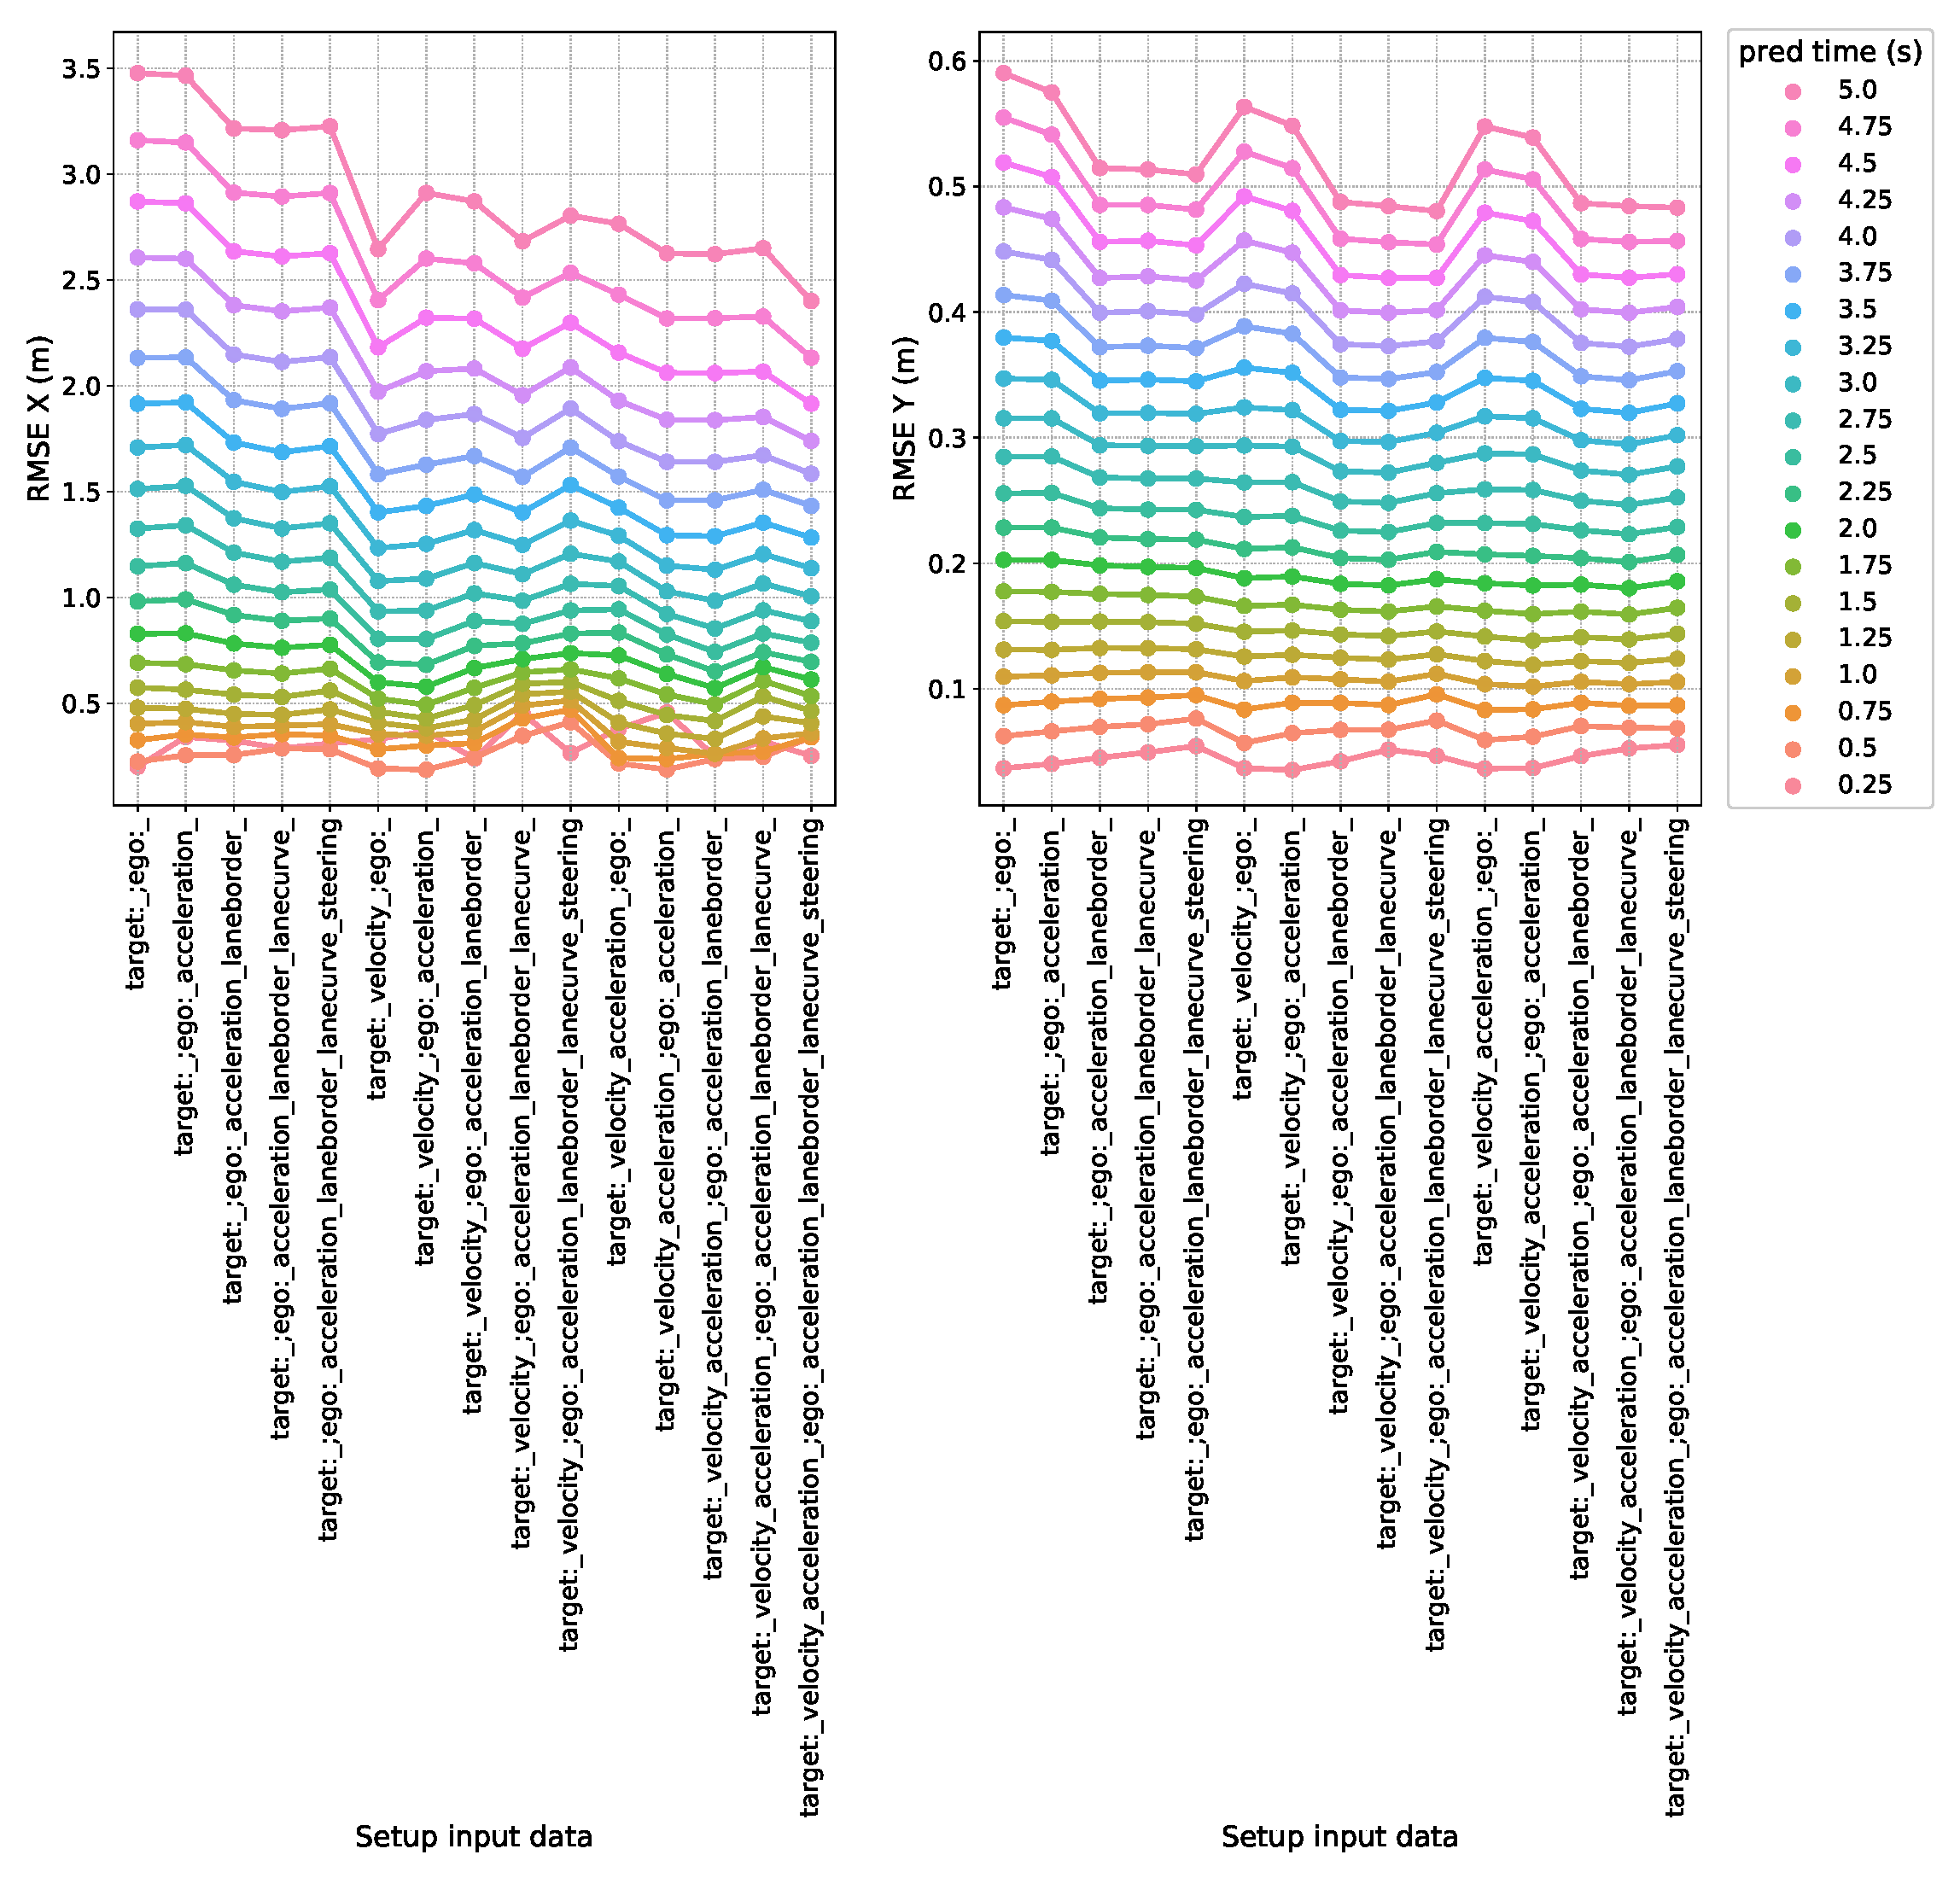
\includegraphics[width=0.95\textwidth]{imgs/lstm_input_data_analysis.eps}
  \caption{Analysis of the \ac{RMSE} for different variations of numerical input to our \ac{LSTM} model trained on the \emph{On-board} data set for \num{8} epochs.}
  \label{fig:lstm_input_data_analysis}
\end{figure}

For the \ac{LSTM}-models, we firstly investigated the composition of the input data to the model to get an idea, what kind of information is useful for the task of motion prediction.
Therefore, we trained several instantiations of our \ac{LSTM}-network architecture on the \emph{On-board} data set $D_1$ for different variations of the input data, for \num{8} epochs each.
Table~\ref{tab:input_data_setups} summarizes the different setups and shows what kind of data is included in each setup shown in Fig.~\ref{fig:lstm_input_data_analysis}.
The simplest setting (setup \num{1}) is using only the positional information of the target vehicle as input and its instantaneous velocity as additional information in the embedding without including any information about the ego-vehicle.
We refer to this setting as the default setting in this section.
In addition, we also analyze settings, where additional information like velocity (setups \num{6}-\num{15}) and acceleration (setups \num{11}-\num{15}) of the target vehicle are available to the system.
Furthermore, if all dynamic information is available relative to the ego-vehicle, there are other features that could be useful for motion prediction such as the current curvature of the road or the current velocity or steering values of the ego-vehicle itself.
For instance, if the ego-vehicle performs a lane change or the road bends, this will influence the relative motion of all other vehicles while this information most likely will not be available from just the positions of the target vehicle. 
On the other hand, if such information is available to the system, it would improve the model's capability of abstracting and inferring correlations between the available information in such situations.
In this evaluation, we include the history of the ego-vehicle's information to the input data and future values to the embedding, whereas we include additional information about the target vehicle to the input data only. 

Figure~\ref{fig:lstm_input_data_analysis} depicts the \ac{RMSE} ($y$-axis) for each input data setup given in table~\ref{tab:input_data_setups} on the $x$-axis at each prediction time step.
Each tick on the $x$-axis corresponds to one input setup, whereas each group of \num{5} ticks from left to right corresponds to one fixed setup for the target vehicle.
The left group contains only the default data about the target vehicle (setups \num{1}-\num{5} in table~\ref{tab:input_data_setups}), the middle group contains the history of the target vehicle's velocity (setups \num{6}-\num{10} in table~\ref{tab:input_data_setups}) and the right group contains additionally the history of the target vehicle's acceleration (setups \num{11}-\num{15} in table~\ref{tab:input_data_setups}).
\begin{center}
    \resizebox{\textwidth}{!}{%
        \begin{tabular}{cccccccc}
            \toprule
            \multirow{2}{1in}{\thead{Setup \#}} & \multicolumn{3}{c|}{\thead{Included target vehicle data}} & \multicolumn{4}{|c}{\thead{Included ego-vehicle data}} \\ 
            \cmidrule{2-8}
             & \thead{Position} & \thead{Velocity} & \thead{Acceleration} & \thead{Acceleration} & \thead{Lane Border} & \thead{Lane Curvature} & \thead{Steering}\\ 
            \midrule
            1 & \checkmark & & & & & &  \\
            \midrule
            2 & \checkmark & & & \checkmark& & &  \\
            \midrule
            3 & \checkmark & & & \checkmark& \checkmark& &  \\
            \midrule
            4 & \checkmark & & & \checkmark& \checkmark& \checkmark&  \\
            \midrule
            5 & \checkmark & & & \checkmark& \checkmark& \checkmark& \checkmark \\
            \midrule
            6 & \checkmark & \checkmark& & & & &  \\
            \midrule
            7 & \checkmark & \checkmark& & \checkmark& & &  \\
            \midrule
            8 & \checkmark & \checkmark& & \checkmark& \checkmark& &  \\
            \midrule
            9 & \checkmark & \checkmark& & \checkmark& \checkmark& \checkmark&  \\
            \midrule
            10 & \checkmark & \checkmark& & \checkmark& \checkmark& \checkmark& \checkmark \\
            \midrule
            11 & \checkmark & \checkmark& \checkmark& & & &  \\
            \midrule
            12 & \checkmark & \checkmark& \checkmark& \checkmark& & &  \\
            \midrule
            13 & \checkmark & \checkmark& \checkmark& \checkmark& \checkmark& &  \\
            \midrule
            14 & \checkmark & \checkmark& \checkmark& \checkmark& \checkmark& \checkmark&  \\
            \midrule
            15 & \checkmark & \checkmark& \checkmark& \checkmark& \checkmark& \checkmark& \checkmark \\
            \bottomrule
        \end{tabular}
    }
    \captionof{table}{Summary of the input data setups of the different models evaluated in Fig.~\ref{fig:lstm_input_data_analysis}.}
	\label{tab:input_data_setups}
\end{center}
Each tick within one group corresponds to one setting for the ego-vehicle, whereas again from left to right the amount of available information increases.
Therefore, the rightmost tick contains information about the ego-vehicle's acceleration, distance to the lane border as well as the curvature of the current lane and its current steering values (setup \num{15} in table~\ref{tab:input_data_setups}). 
We observe that adding more information about both, the ego- and target vehicle, indeed improves prediction accuracy significantly: the difference between the best and worst setting is more than \SI{1}{\meter} in $x$-direction and more than \SI{0.1}{\meter} in $y$-direction.
For both dimensions, setup \num{15} using all available information outperforms the simpler setups.
However, there are some interesting peculiarities visible in this analysis that are worth noting.
For instance, the input information improving performance in $x$-direction the most appears to be the target vehicle's velocity (setups \num{1}-\num{5} vs. setups \num{6}-\num{10}). 
\begin{figure}[t!]
	\centering
    \subfloat[\label{subfig:lstm_units_analysis}]{%
        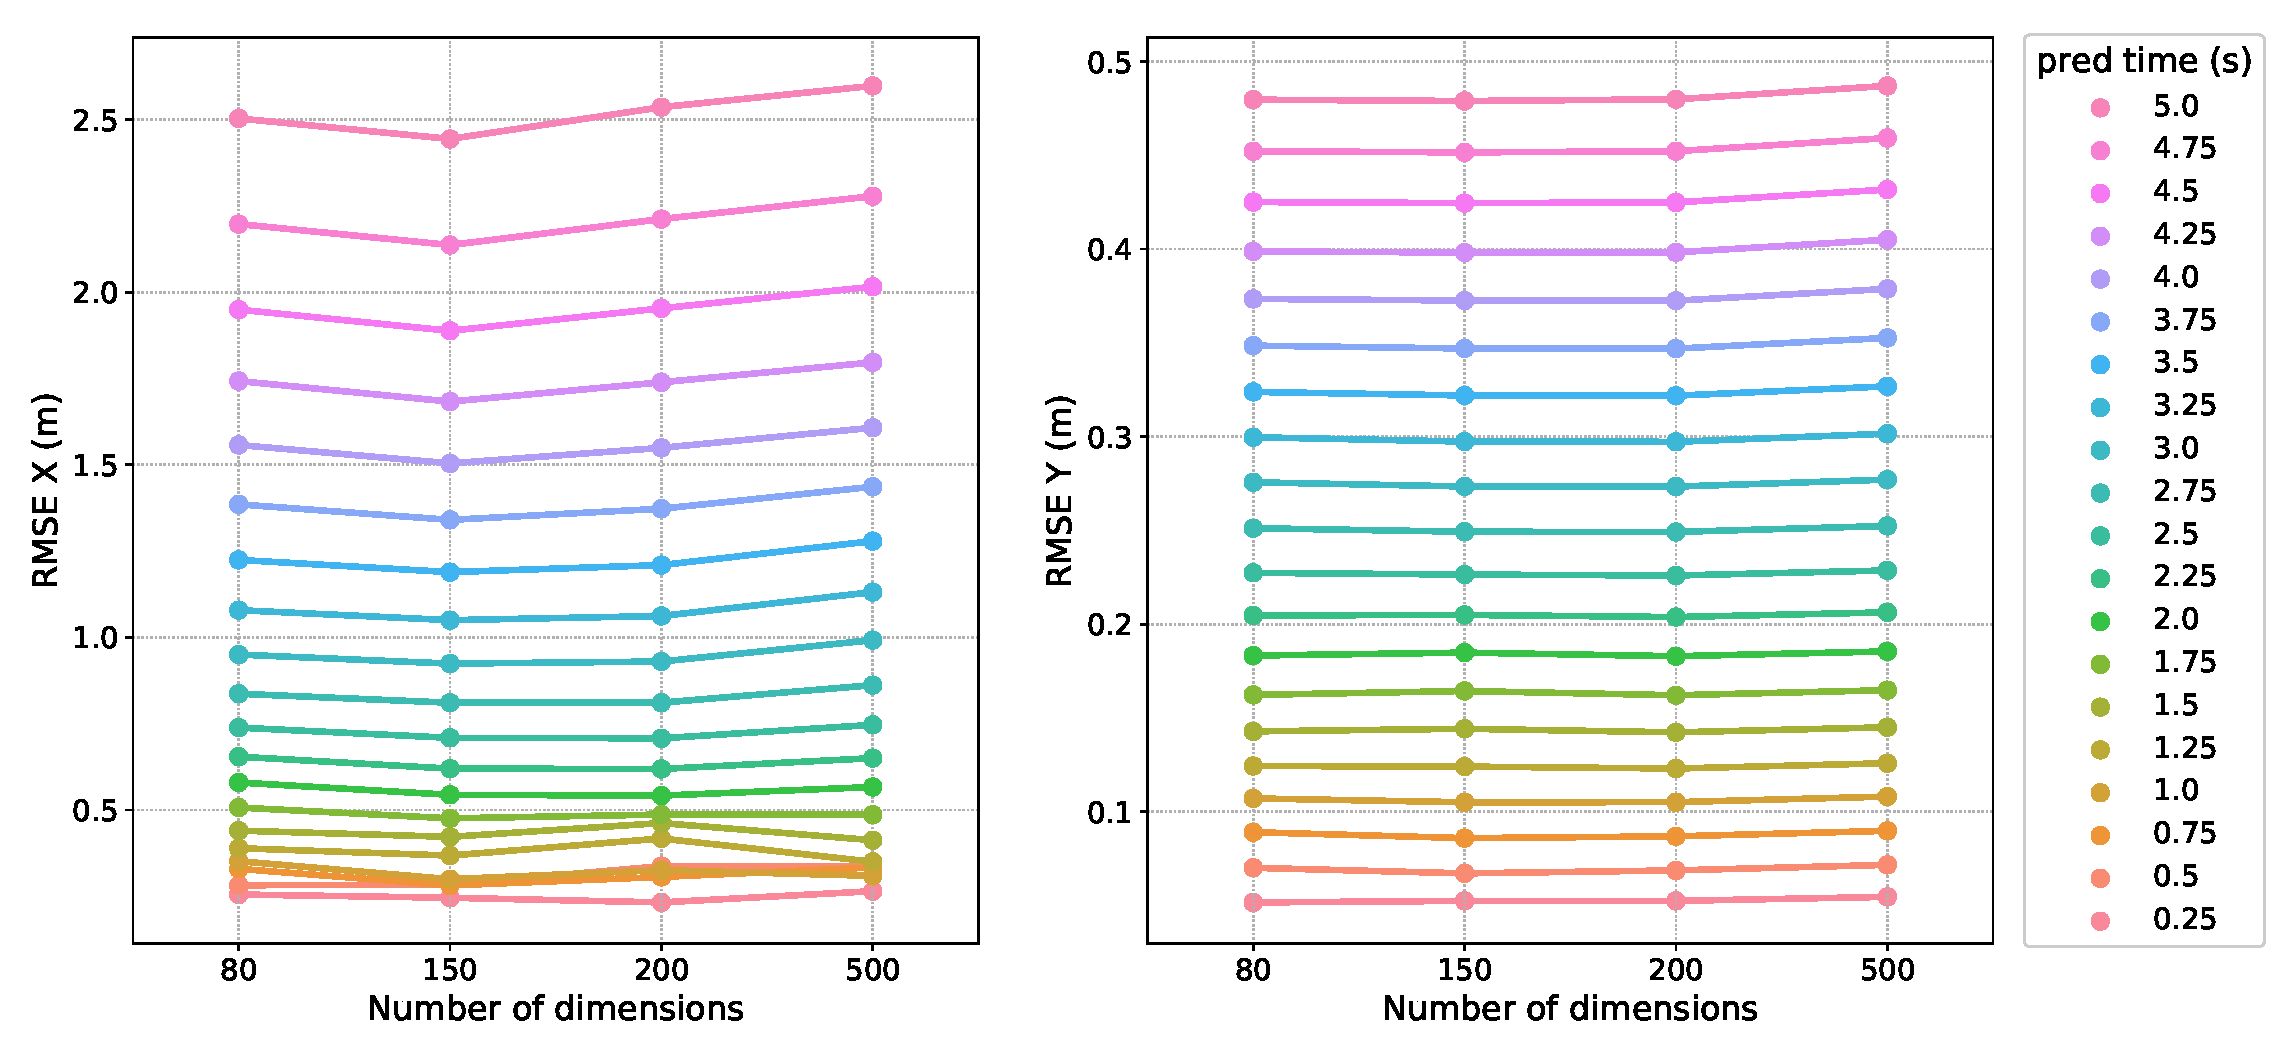
\includegraphics[width=\columnwidth]{imgs/lstm_units_analysis.eps}
    }
    \vspace{-0.3cm}
    \subfloat[\label{subfig:lstm_layers_analysis}]{%
        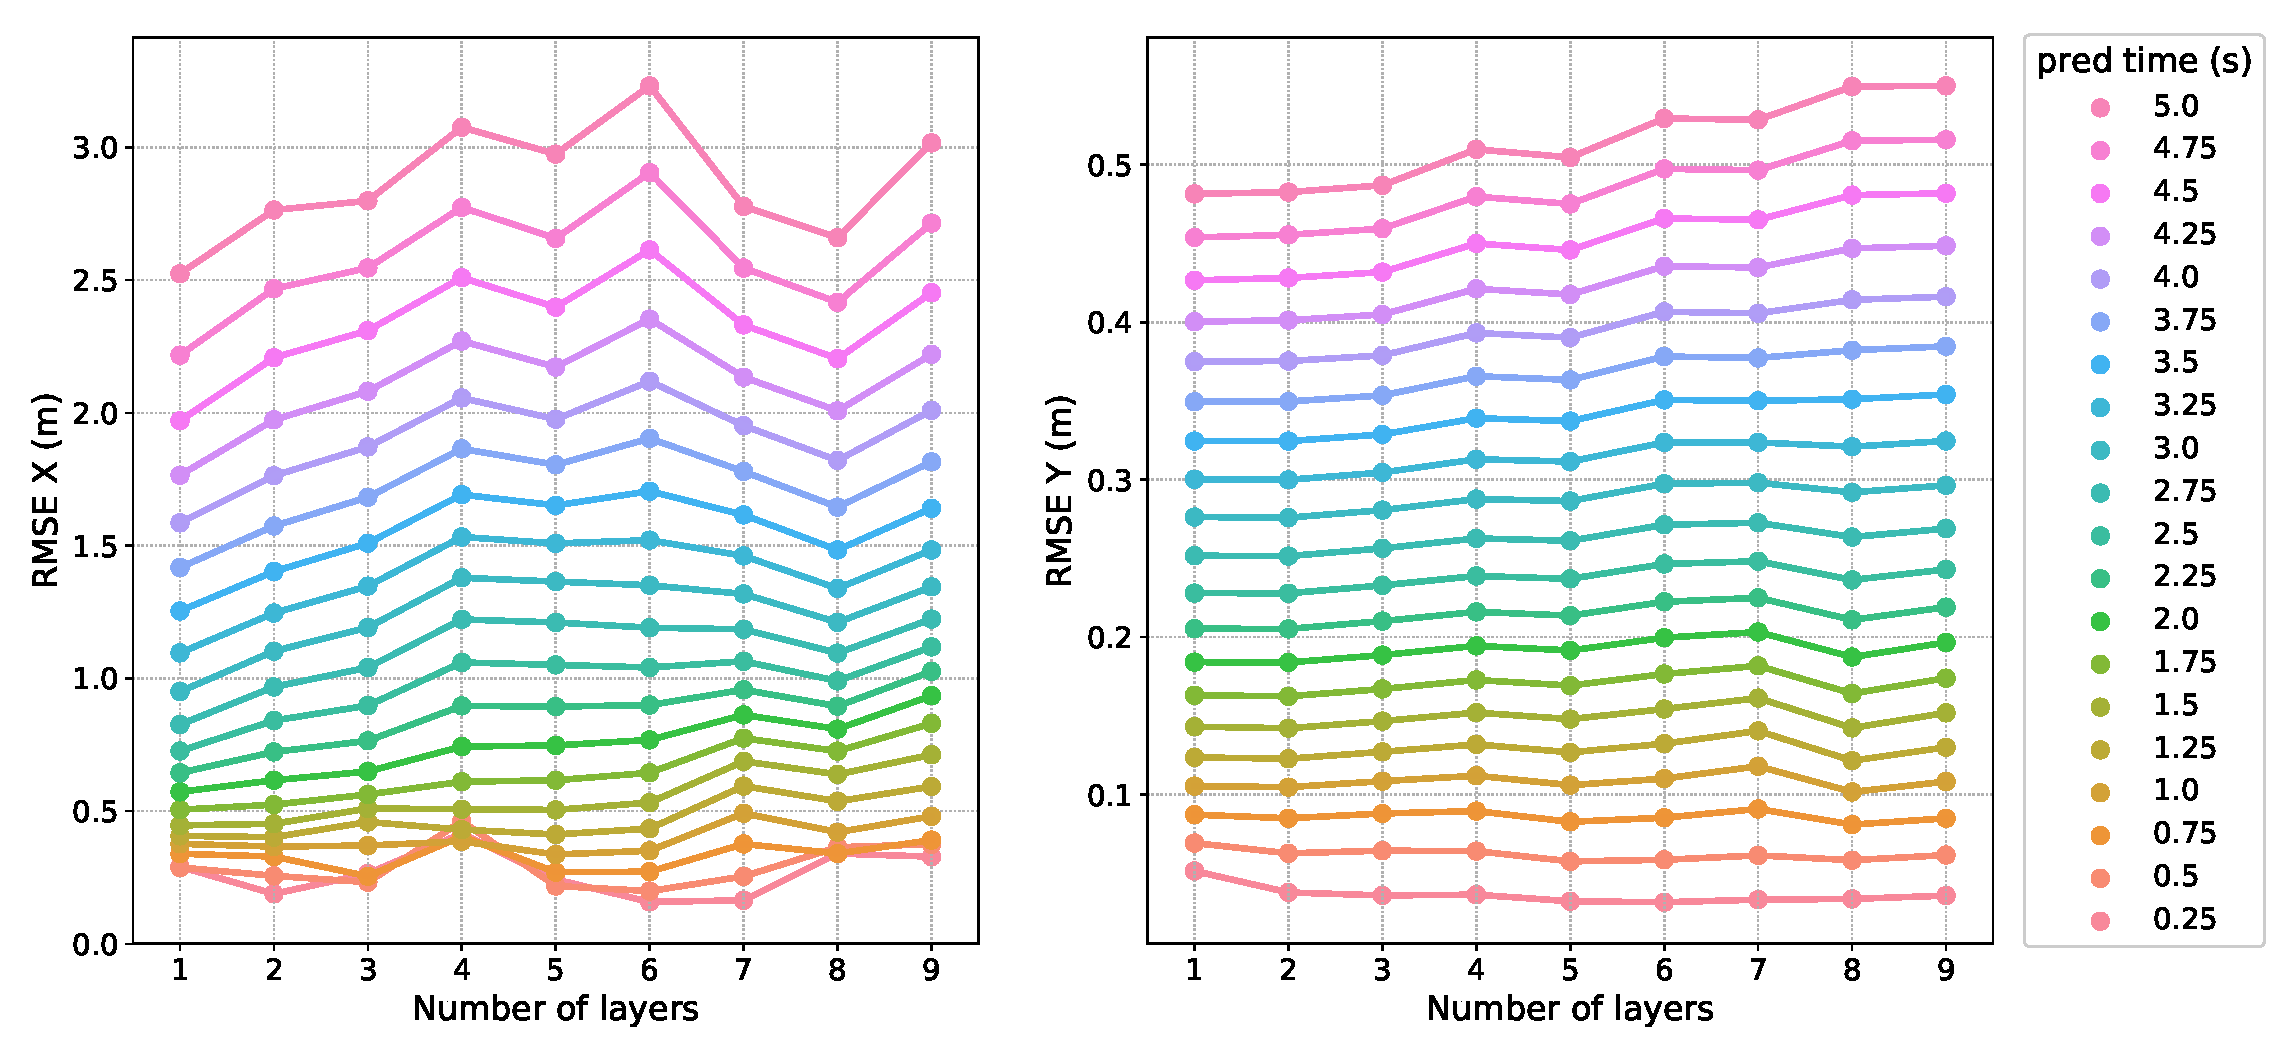
\includegraphics[width=\columnwidth]{imgs/lstm_layers_analysis.eps}
    }
    \caption{Visualization of the \ac{RMSE} for different parameter tests of our \ac{LSTM}-model trained on the \emph{On-board} data set for \num{8} epochs:~\protect\subref{subfig:lstm_units_analysis} depicts the \ac{RMSE} when varying the number of dimensions in each \ac{LSTM} cell~\protect\subref{subfig:lstm_layers_analysis} visualizes the \ac{RMSE} when varying the number of layers, i.e., the number of encoder and decoder \ac{LSTM} cells are used in the network.}
    \label{fig:lstm_units_layers_analysis}
\end{figure}
Furthermore, the target vehicle's acceleration does not yield further significant improvements given its velocity is available.
Interestingly, setup \num{6} using only the target vehicle's velocity as additional information is closely behind the best setting in $x$-direction.
Furthermore, the performance boost of the setting using all available information (setup \num{15} or the rightmost tick) over the prior setting comes from the ego-vehicle's steering, which only appears when its acceleration information is also available.
For the $y$-direction, we observe similar trends in that the target vehicle's acceleration does not yield significant improvements if its velocity is already given.
Here however, the information about the ego-vehicle's distance to the lane borders appears to be the input that gives the most significant improvements in $y$-direction (setup \num{2} vs. \num{3}, setup \num{7} vs. \num{8} and setup \num{12} vs. \num{13}).
That makes sense, since these inputs encode information about the ego-vehicle's motion in $y$-direction when, for instance, performing lane changes.
As setup \num{15} using all available information (the rightmost tick in Fig.~\ref{fig:lstm_input_data_analysis}) is by far outperforming all other settings in $x$-direction and is on par with the best in $y$-direction, we use this data setup for further analyzing the hyperparameters of the \ac{LSTM}-model.

\begin{figure}[t!]
  \centering
  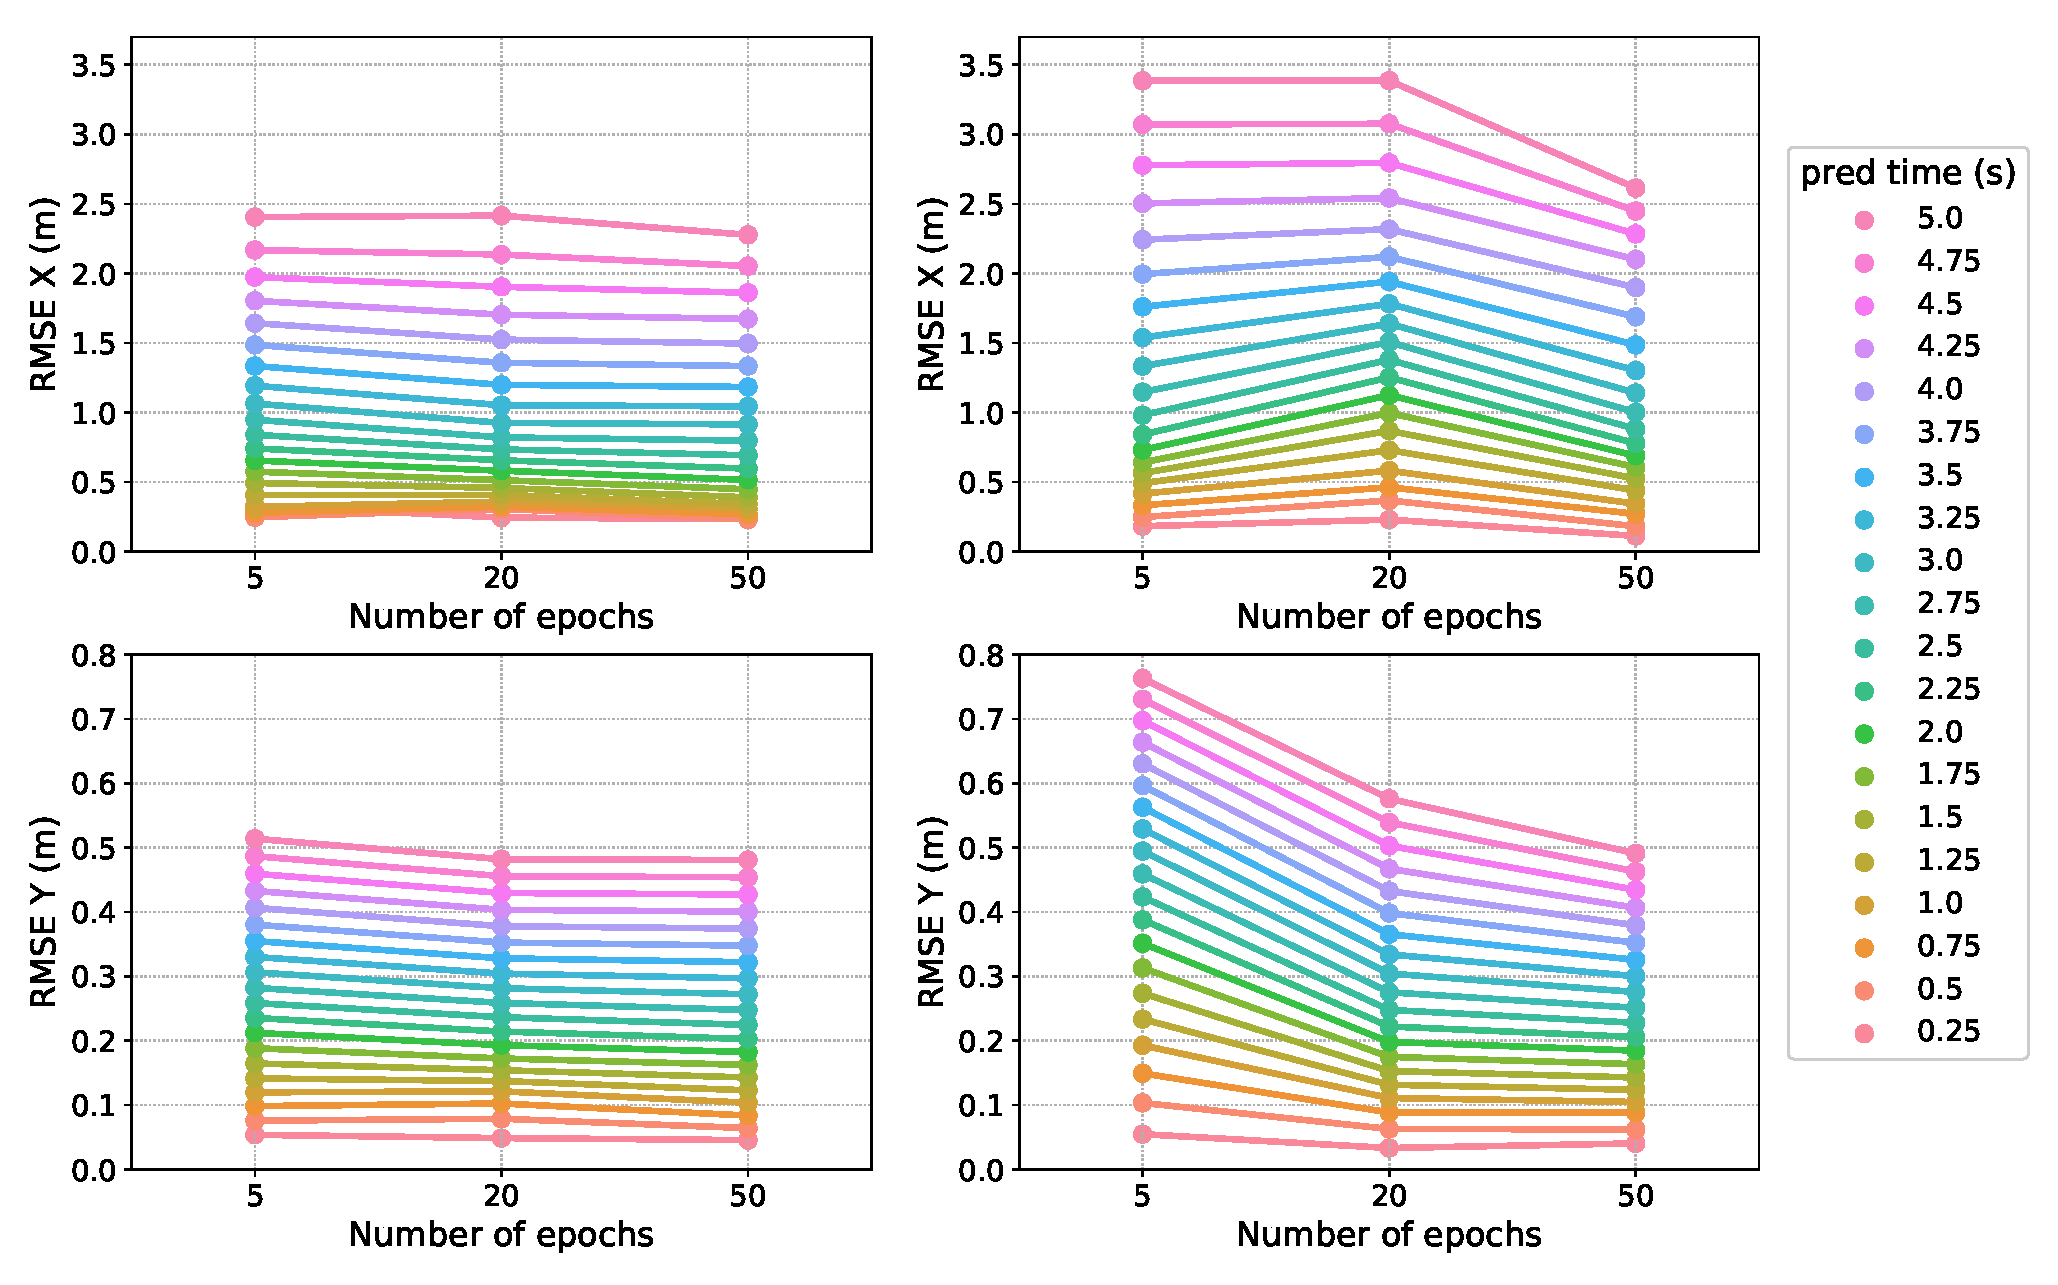
\includegraphics[width=0.9\textwidth]{imgs/lstm_layers_epochs_analysis.eps}
  \caption{Analysis of the \ac{RMSE} varying the number of layers and epochs of our \ac{LSTM} model trained on the \emph{On-board} data set. The left column shows the \ac{RMSE} of a model with only one layer trained for \num{5}, \num{20} and \num{50} epochs, while the right column shows the \ac{RMSE} of a model with \num{10} layers trained for \num{5}, \num{20} and \num{50} epochs.}
  \label{fig:lstm_layers_epochs_analysis}
\end{figure}

We continue our hyperparameter analysis by inspecting the number of dimensions within the \ac{LSTM} cells.
In our initial experiment, we used \num{80} dimensions in each of the \ac{LSTM} encoder and decoder cell.
Here, we investigate if adding more dimensions improves the models' prediction performance.
Again, we train the model for \num{8} epochs.
Figure~\ref{subfig:lstm_units_analysis} depicts the \ac{RMSE} for models with \num{80}, \num{150}, \num{200} and \num{500} dimensions in the \ac{LSTM} cells.
We observe that the model with \num{150} dimensions performs best in $x$-direction whereas all models show comparable performance in $y$-direction.
However, increasing the number of dimensions beyond \num{150} per \ac{LSTM} does not improve the models' accuracy but rather deteriorates the performance.
Therefore, we fix the number of dimensions within the \ac{LSTM} cells to \num{150} for further investigation.

In the next step, we inspect how the number of layers in our network architecture influences the model's performance.
Here, one layer is a pair of one \ac{LSTM} encoder and decoder cell each.
Thus, a model with \num{2} layers consists of a sequence of \num{2} \ac{LSTM} encoder cells followed by a sequence of again \num{2} \ac{LSTM} decoder cells.
Figure~\ref{subfig:lstm_layers_analysis} visualizes the \ac{RMSE} of models with \num{1} up to \num{9} layers trained for \num{8} epochs.
This analysis shows that the model using only one layer performs best and that increasing the number of layers and thus using a deeper network architecture does not improve the model's performance.
On the contrary, more layers lead to worse accuracy in both dimensions.
However, we trained all models for a fixed number of \num{8} epochs whereas deeper network architectures might demand a longer training process.

In the next step, we therefore analyze the number of layers and number of epochs jointly to investigate if larger network architectures trained for more epochs improve prediction performance.
Figure~\ref{fig:lstm_layers_epochs_analysis} visualizes the results of this experiment: the left column depicts the \ac{RMSE} of a model with only one layer trained for \num{5}, \num{20} and \num{50} epochs, whereas the right column shows the \ac{RMSE} of a model with \num{10} layers trained for \num{5}, \num{20} and \num{50} epochs. 
We observe that training a deeper model for more epochs does improve its accuracy.
However, if we compare the left and right plots in Fig.~\ref{fig:lstm_layers_epochs_analysis}, we also find that by training a model with \num{10} layers for \num{50} epochs we only achieve the accuracy of the simpler single-layer \ac{LSTM} model trained for \num{5} epochs.
We conclude, that using more layers even with a longer training process (i.e., increased number of epochs) does not lead to improved prediction results.
Thus, a \ac{LSTM} model with one encoder and decoder cell each is not only the simplest network architecture but also the best in terms of accuracy and time needed for training.

\begin{figure}[t!]
  \centering
  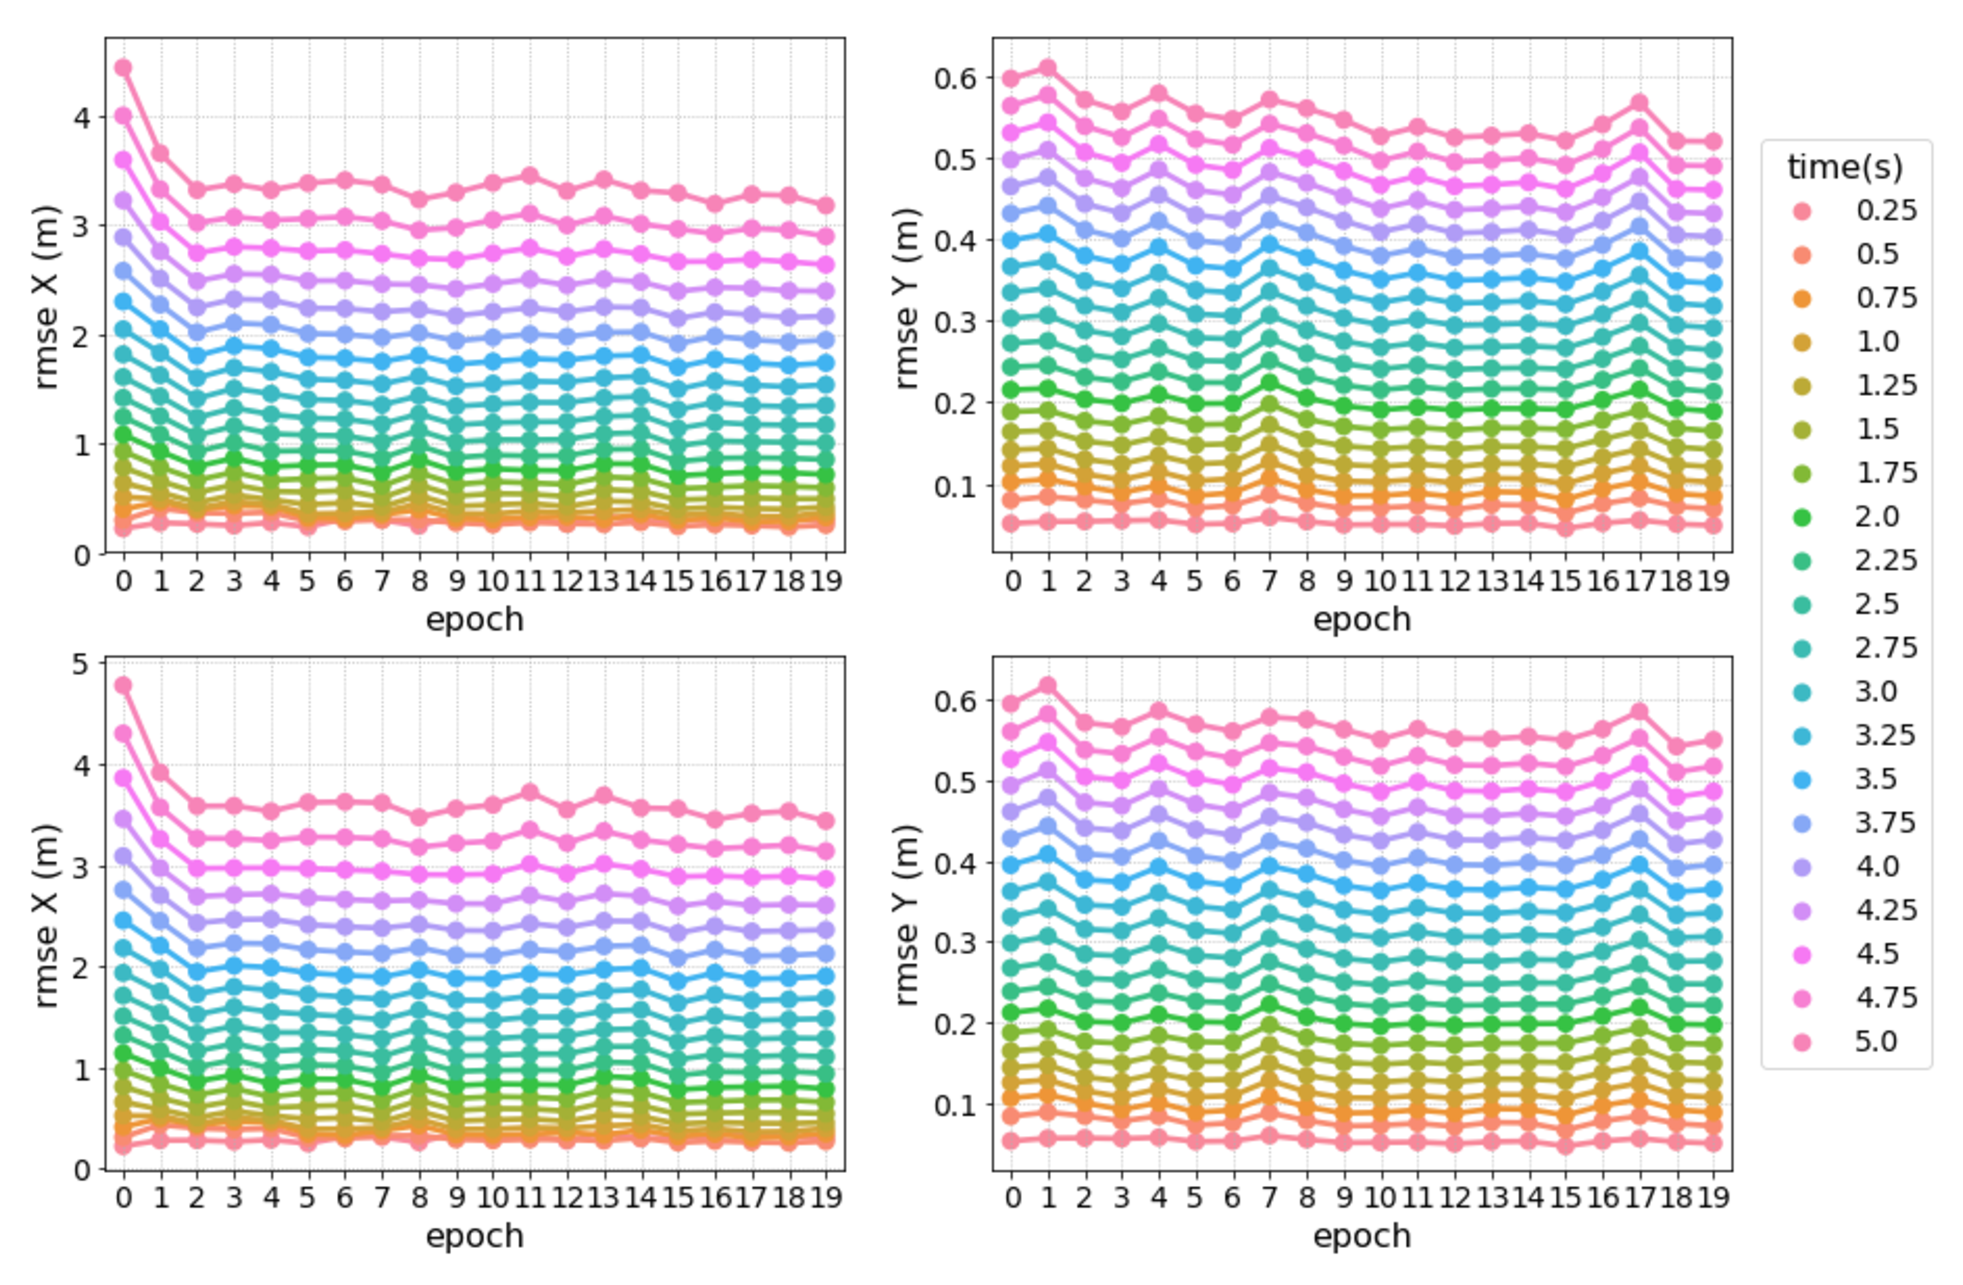
\includegraphics[width=0.95\textwidth]{imgs/rmse_dev_over_epochs.eps}
  \caption{Development of the \ac{RMSE} at every prediction time step during the training process of the \ac{LSTM} \acs{SPA} \num{3} model for each epoch on the training (left column) and validation part (right column) of the \emph{On-board} data set.
  One observes comparable trends on both, training and validation set and that the \ac{RMSE} does not significantly decrease after \num{10} epochs.}\label{fig:rmse_dev_over_epochs}
\end{figure}

We briefly summarize the findings of this section and fix the following set of parameters for subsequent sections: we use a \ac{LSTM} model with one encoder and one decoder cell with \num{150} hidden dimensions each.

\subsubsection{Model training}%
\label{ssubsec:model_training_lstms}

Using the aforementioned network architecture and hyperparameter set, we train one model instantiation for each encoding scheme mentioned in section~\ref{subsec:scene_representation_in_vectors}, whereas only the input dimensionality of the encoder cell changes when varying the representation of the input data.
Importantly, we focus on positional information as the only input for our \ac{LSTM} models in this work for reasons of consistency to make all models as comparable as possible.
Hence, we neglect for example the history of the target (or ego-) vehicle's velocity or acceleration as input here.
Between the two data sets, the only difference between models is the auxiliary data, that is used as additional input to the \ac{LSTM} decoder cell at each time step.
For both data sets, we use the instantaneous velocity of the target vehicle to aid the model predicting the future trajectory at every time step.
As there is no ego-vehicle present in the \emph{\ac{NGSIM}} data set $D_2$, we use no further auxiliary data.
For the \emph{On-board} data set $D_1$, we use the ego-vehicle's predicted acceleration and the estimated curvature of the ego-vehicle's current lane.
Although this is future information, we argue that it is solely about the ego-vehicle, which we expect to be available at the time the prediction is to happen.
We assume, that an automated vehicle, in order to safely navigate, will have an estimation of the future lane curvature as well as the acceleration values of its own planned trajectory.
Furthermore, we employed early stopping, that is, we trained our models for \num{10} epochs as we found that the models' performance stagnate on both, training and validation data sets, when training for up until a total \num{20} epochs.
Figure~\ref{fig:rmse_dev_over_epochs} visualizes this result by showing the development of the \ac{RMSE} of the \ac{LSTM} \acs{SPA} \num{3} model using the \ac{SPA}-power-with-ego vector representation $(\mathbf{S}_{t}^{ego})_{t_0}^{t_N}$ as input for the training (Fig.~\ref{fig:rmse_dev_over_epochs} left column) and validation part (Fig.~\ref{fig:rmse_dev_over_epochs} right column) of the \emph{On-board} data set $D_1$.
On the $y$-axis of each sub-figure, we have the \ac{RMSE} while the $x$-axis from left to right depicts the result after each epoch during the training process.
Each colored line illustrates the \ac{RMSE} of the model for one particular prediction time step while all points with the same value on the $x$-axis depict the model's performance after the respective epoch during the training process.

\subsubsection{Evaluation}%
\label{ssubsec:evaluation_lstms}

\begin{figure}[t!]
	\centering
    \subfloat[\label{subfig:lstm_rmse_all_on_board}]{%
        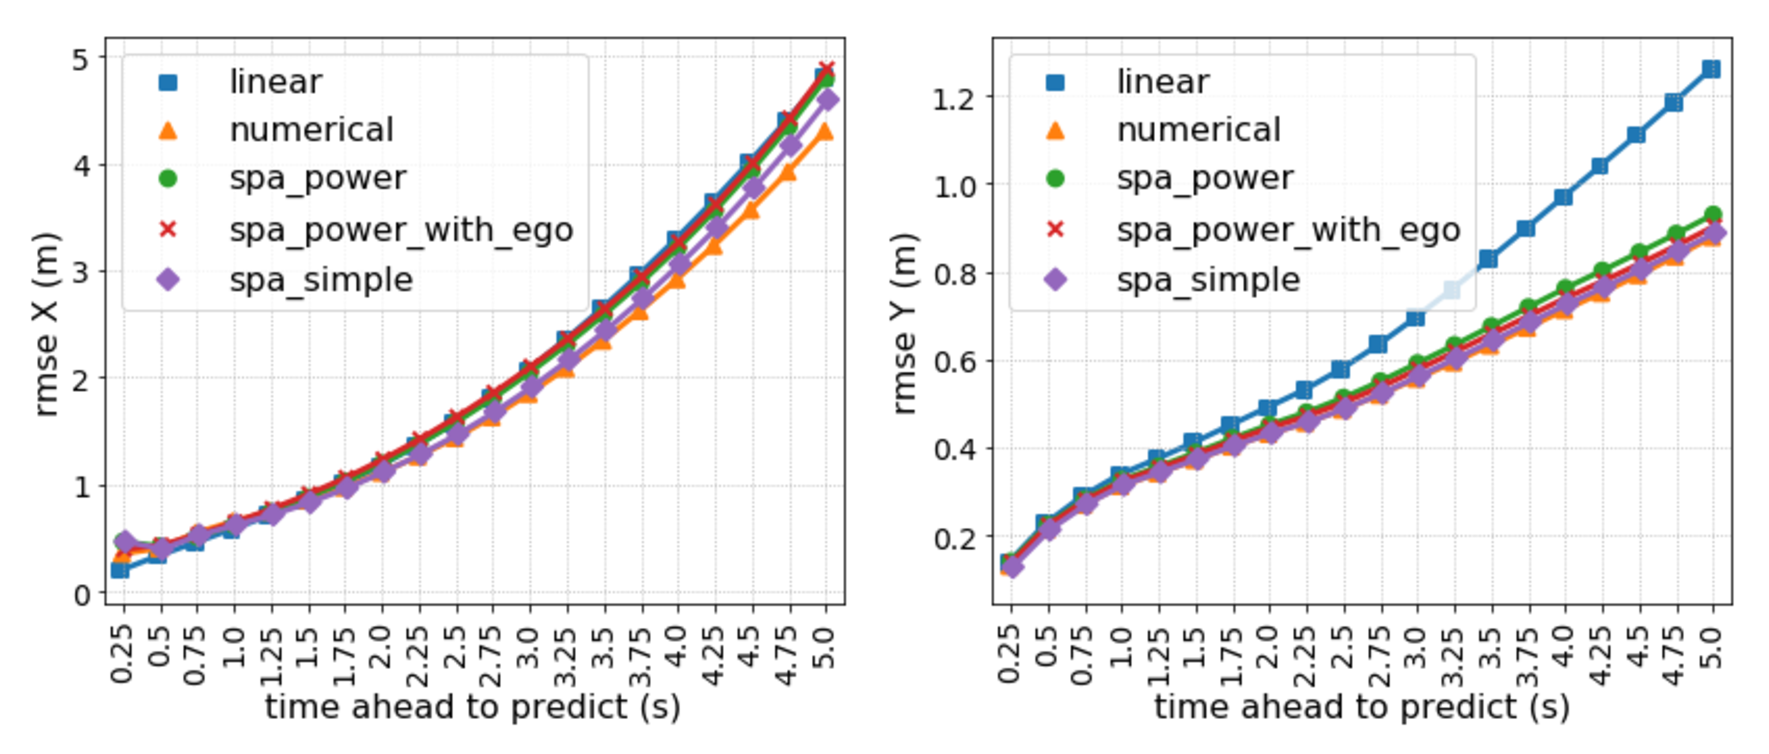
\includegraphics[width=0.5\columnwidth]{imgs/rmse_large_all.eps}
    }
    %\vspace{-0.3cm}
    \subfloat[\label{subfig:lstm_rmse_subset_on_board}]{%
        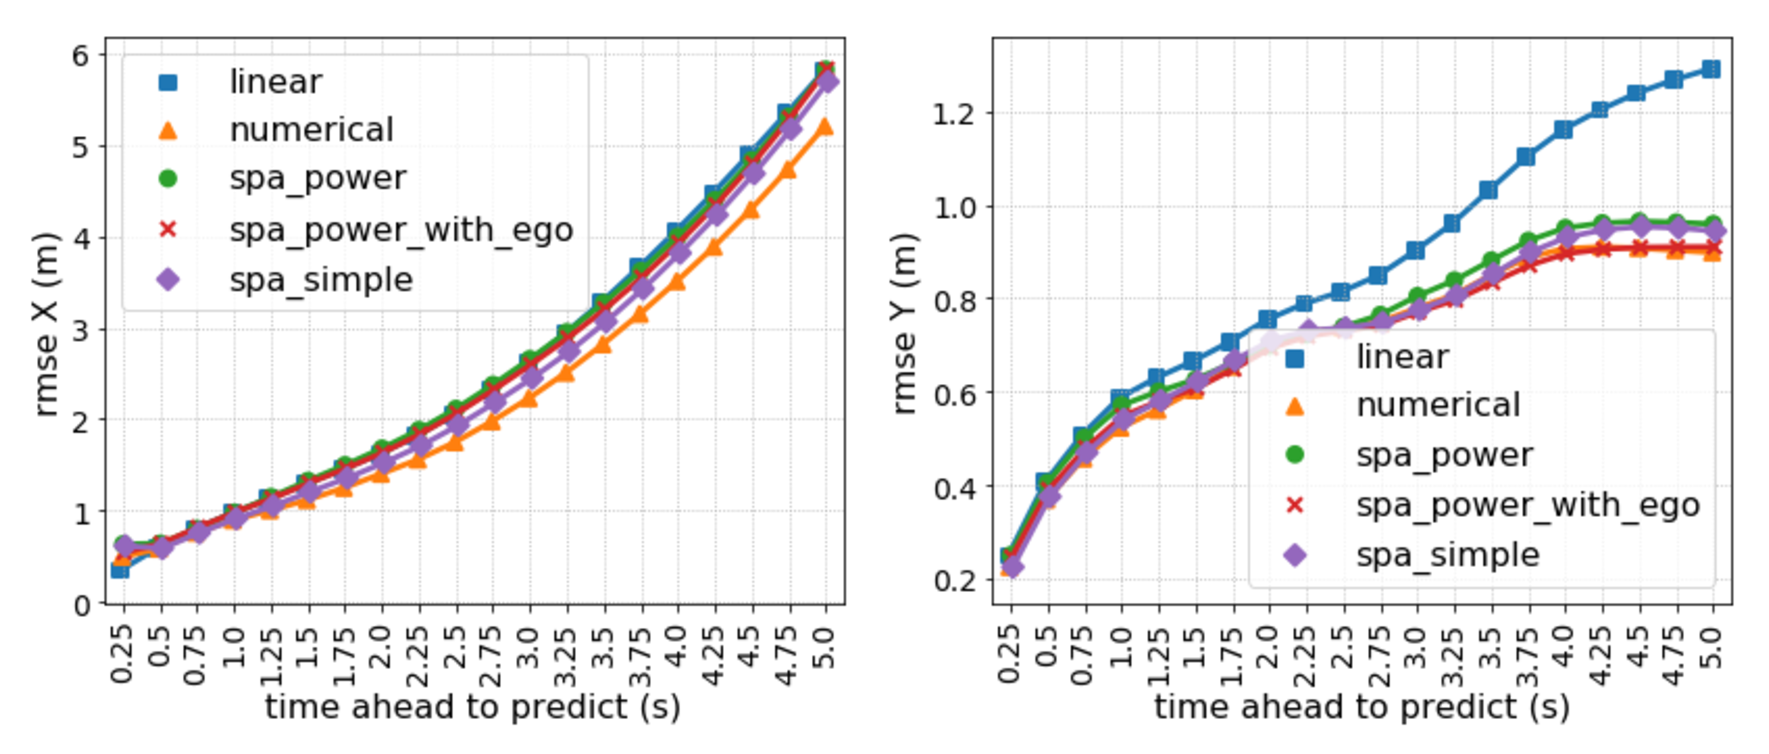
\includegraphics[width=0.5\columnwidth]{imgs/rmse_large_subset.eps}
    }
    \caption{Visualization of the \ac{RMSE} of all \ac{LSTM} models on the \emph{On-board} data set:~\protect\subref{subfig:lstm_rmse_all_on_board} shows the complete validation set $V_1 \subset D_1$~\protect\subref{subfig:lstm_rmse_subset_on_board} shows the subset of situations with at least \num{3} other vehicles present and distance between the target and ego-vehicle lower than  \SI{20}{\meter} and between target and closest other vehicle lower than \SI{10}{\meter}.}\label{fig:rmse_on_board_all}
\end{figure}

Figure~\ref{fig:rmse_on_board_all} visualizes the \ac{RMSE} of all \ac{LSTM}-based models on the validation-set $V_1 \subset D_1$ of the \emph{On-board} data set using \num{512}-dimensional vectors.
Figure~\ref{subfig:lstm_rmse_all_on_board} shows the performance on the complete validation-set, whereas Fig.~\ref{subfig:lstm_rmse_subset_on_board} depicts only situations with at least \num{3} other vehicles present, the distance between the target and the ego-vehicle being lower than \SI{20}{\meter} and the distance between the target and the closest other vehicle being less than \SI{10}{\meter}.
We observe that all approaches yield comparable results with notable differences in certain situations.
Although the models employing the \ac{SPA}-power encoding schemes tend to perform worst in $x$-direction, we observe that they perform better in $y$-direction in crowded situations with closely driving vehicles with the \acs{LSTM} \acs{SPA} \num{3} model ranking best along the \acs{LSTM} numerical model.
\begin{figure}[t!]
    \centering
    \subfloat[\label{subfig:histogram_on_board_1}]{%
        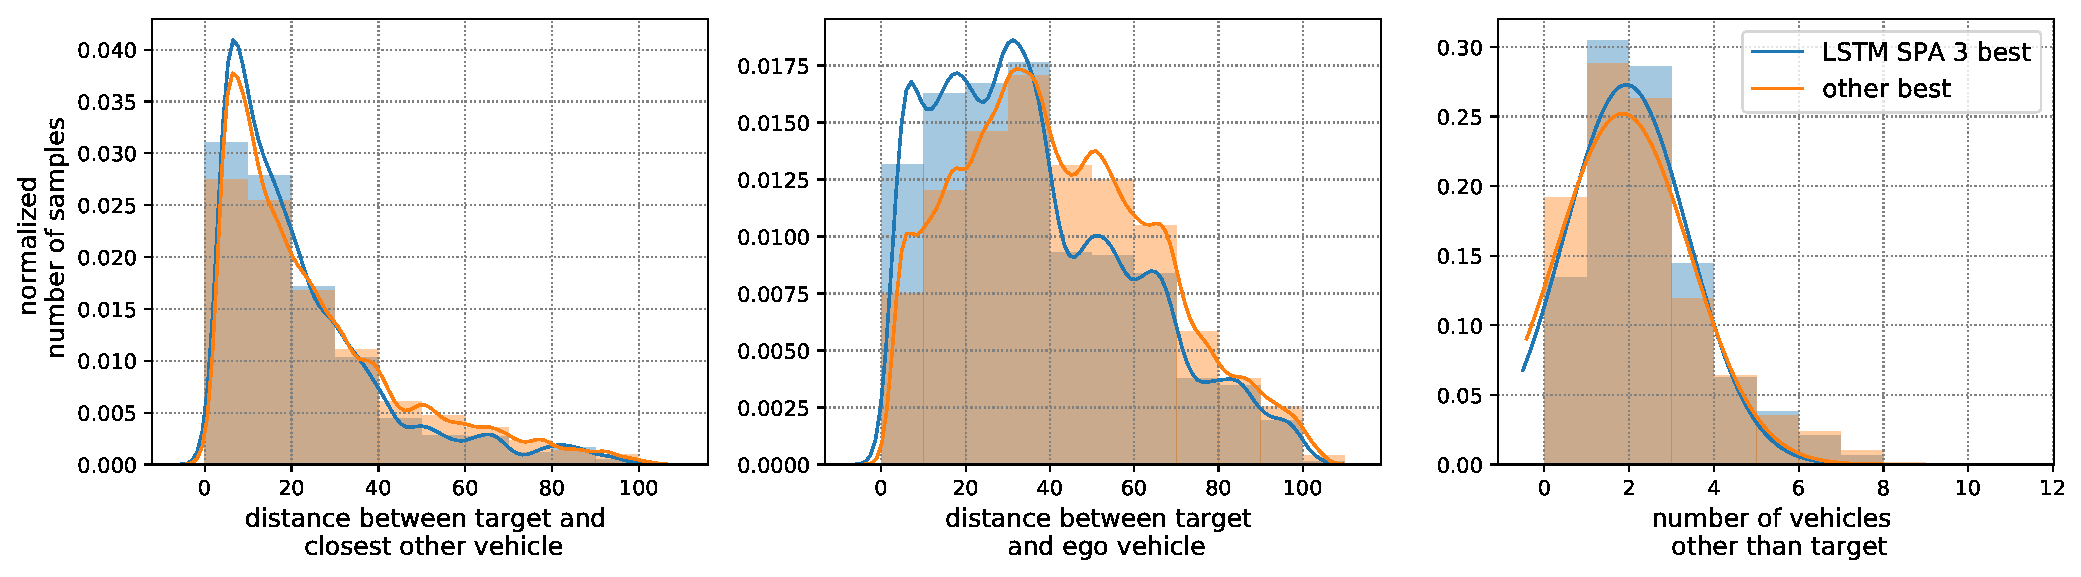
\includegraphics[width=0.95\linewidth]{imgs/histogram_on_board_1.eps}
    }\\
    \subfloat[\label{subfig:histogram_on_board_2}]{%
        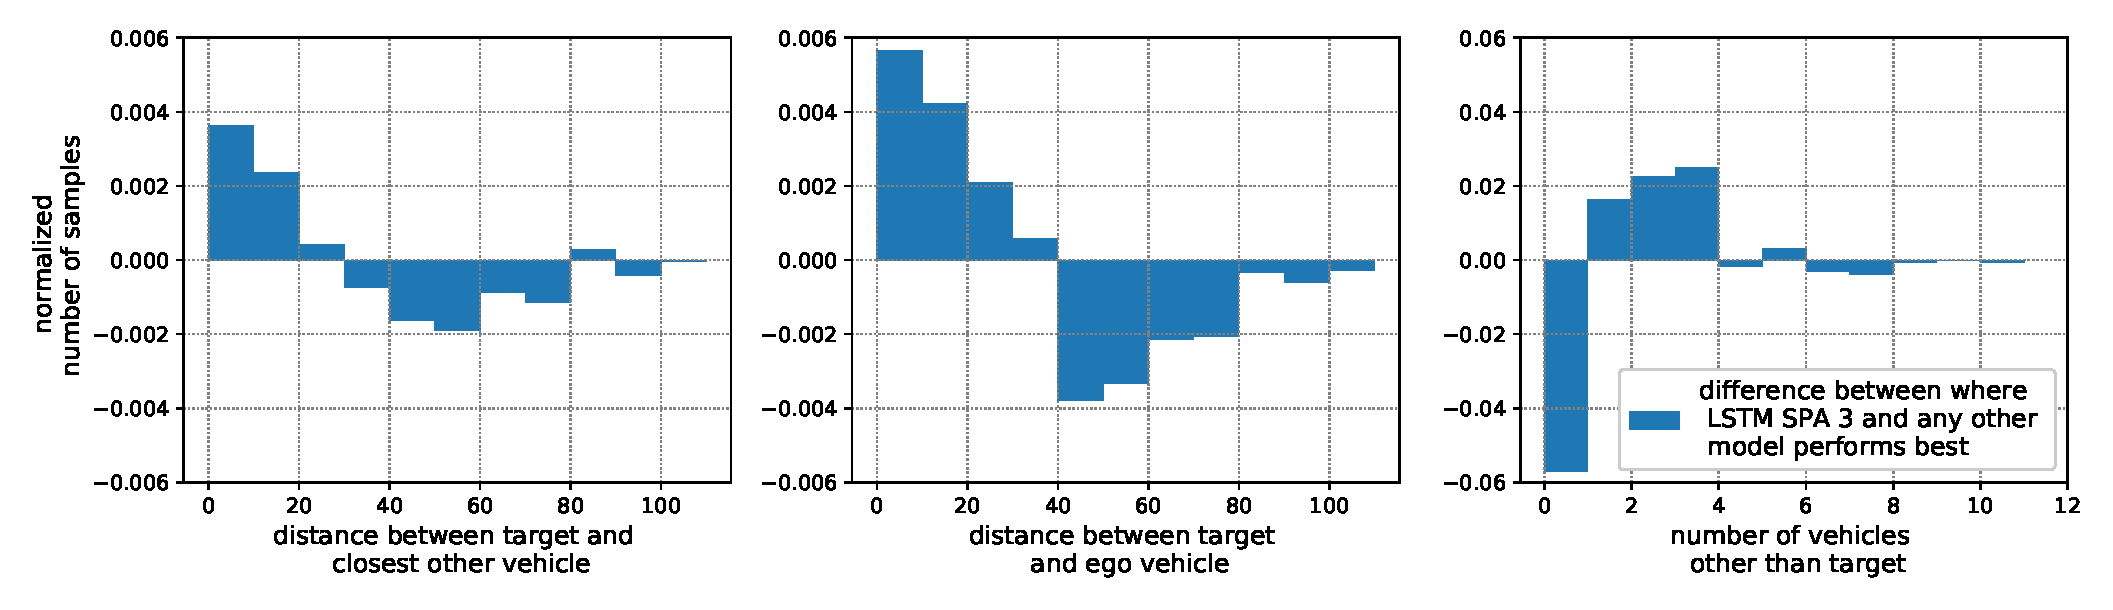
\includegraphics[width=0.95\linewidth]{imgs/histogram_on_board_2.eps}
    }
    \caption{Metric evaluation specifying situations where the \ac{LSTM} \acs{SPA} \num{3} model outperforms all other approaches regarding the \acs{RMSE} in $y$-direction on the \emph{On-board} data set $D_1$.
      In the upper row~\protect\subref{subfig:histogram_on_board_1}, blue bars illustrate samples where \ac{LSTM} \ac{SPA} \num{3} performs better than all other models while the orange bars depict samples where any other model performs best.
      From left to right, the plots in ~\protect\subref{subfig:histogram_on_board_1} illustrate the distance between the target vehicle and the closest other vehicle, the distance between the target and the ego-vehicle and the number of vehicles other than the target.
      The lower row~\protect\subref{subfig:histogram_on_board_2} illustrates the difference between the blue and orange bars in the corresponding plot in~\protect\subref{subfig:histogram_on_board_1}.
    }
    \label{fig:histograms_on_board}
\end{figure}

To further investigate this result, we evaluated certain metrics, chosen to characterize crowded and potentially dangerous situations, for items in the validation set, where the \ac{LSTM} \ac{SPA} \num{3} model outperforms all other approaches with respect to the \ac{RMSE} in $y$-direction (see Fig.~\ref{fig:histograms_on_board}).
We observe that the number of samples, where the distance between the target and the ego-vehicle and/or the closest other object being small is significantly higher when the \ac{LSTM} \ac{SPA} \num{3} model outperforms all other approaches.
For samples where the \ac{LSTM} \ac{SPA} \num{3} model performs best, the number of samples with a distance less than \SI{20}{\meter} between the target and ego-vehicle is \SI{50.5}{\percent} higher compared to samples where any of the other models performs best.
For distances less than \SI{20}{\meter} between the target vehicle and the closest other vehicle, the number of samples is still \SI{11.4}{\percent} higher when the \ac{LSTM} \ac{SPA} \num{3} model performs best.
Finally, the number of situations with at least \num{3} other vehicles present is also \SI{7.8}{\percent} higher compared to samples where any other model performs best.
However, we aim to investigate more sophisticated options such as clustering methods in future work to uncover other, potentially more meaningful features compared to the ones shown in this paper, distinguishing between situations where \ac{LSTM} \ac{SPA} \num{3} performs best compared to another model showing the best performance.

\begin{figure}[t!]
	\centering
    \subfloat[\label{subfig:lstm_rmse_512_ngsim}]{%
        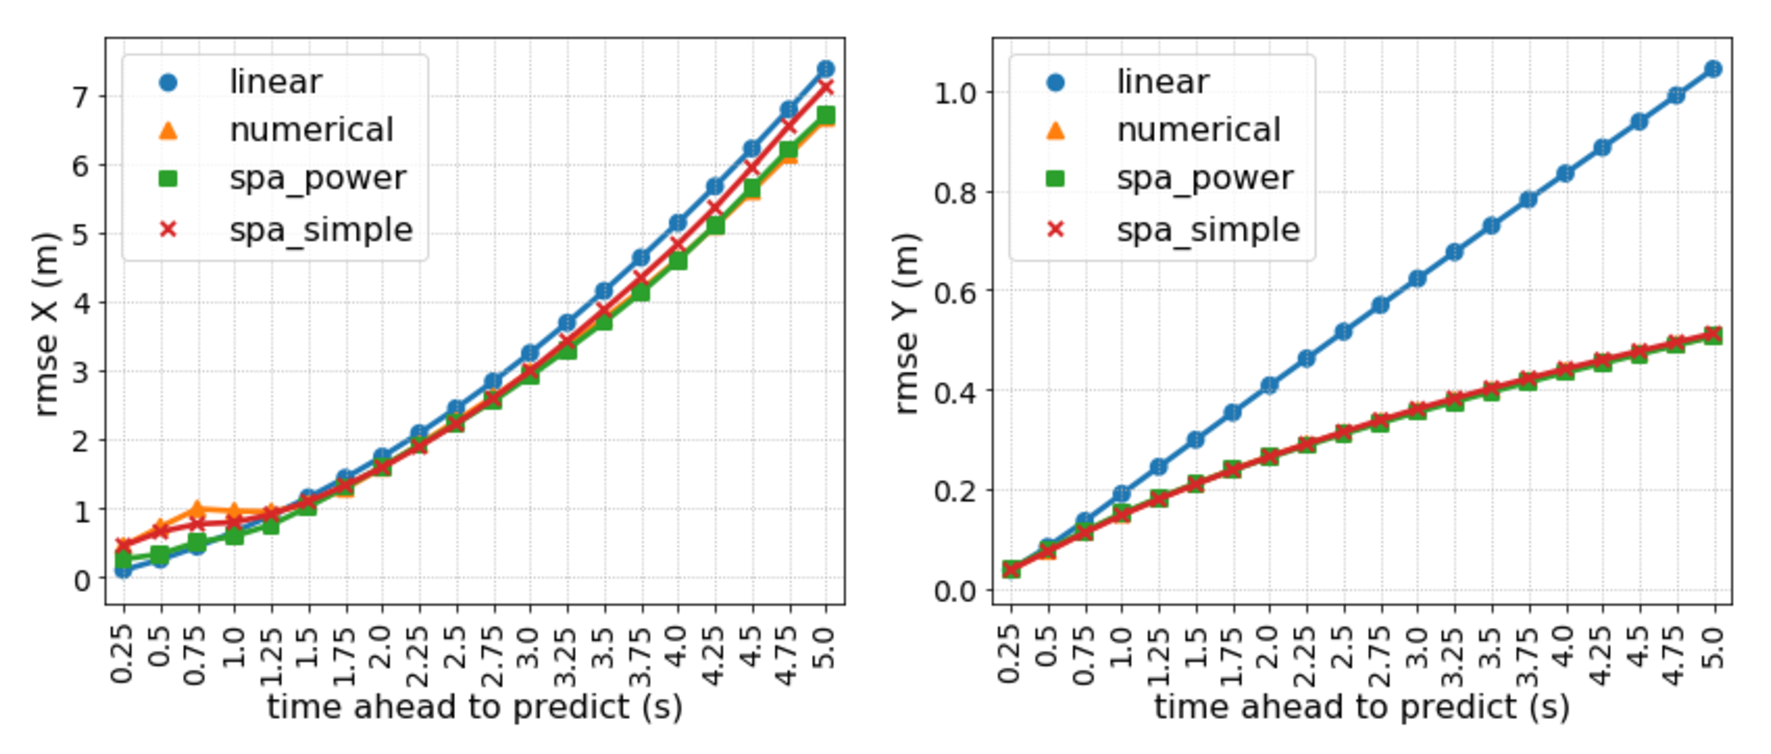
\includegraphics[width=0.5\columnwidth]{imgs/rmse_ngsim_512_10epochs.eps}
    }
    \subfloat[\label{subfig:lstm_rmse_1024_ngsim}]{%
        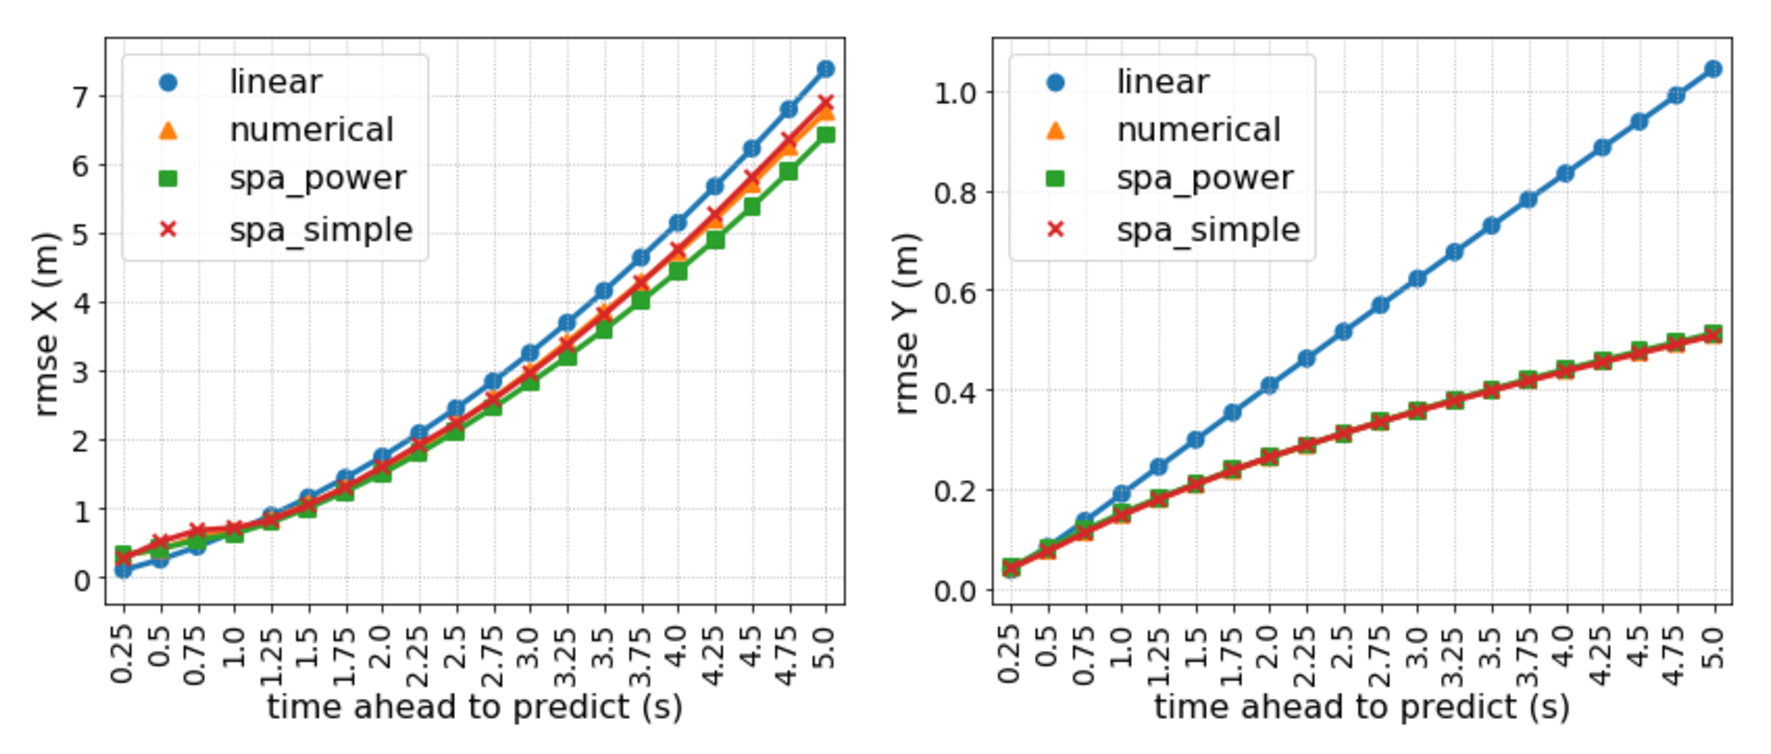
\includegraphics[width=0.5\columnwidth]{imgs/rmse_ngsim_1024_10epochs.eps}
    }

    \caption{Visualization of the \ac{RMSE} of all \ac{LSTM} models on the \emph{\ac{NGSIM}} validation set $V_2 \subset D_2$ using~\protect\subref{subfig:lstm_rmse_512_ngsim} vectors of dimension $512$ for the \ac{SPA}-based models and~\protect\subref{subfig:lstm_rmse_1024_ngsim} using vectors of dimension $1024$ for the \ac{SPA}-based models.}\label{fig:rmse_ngsim_all}

\end{figure}

Figure~\ref{fig:rmse_ngsim_all} visualizes the \ac{RMSE} of all \ac{LSTM}-based models on the validation-set $V_2 \subset D_2$ of the \emph{\ac{NGSIM}} data set for \num{512}-dimensional vectors (Fig.~\ref{subfig:lstm_rmse_512_ngsim}) and for \num{1024}-dimensional vectors (Fig.~\ref{subfig:lstm_rmse_1024_ngsim}).
We observe, that all \ac{LSTM} models achieve a very similar performance (almost identical in $y$-direction) with \ac{LSTM} \ac{SPA} \num{1} achieving the best performance in $x$-direction being on par with the numerical encoding for \num{512}-dimensional vectors.
For \num{1024}-dimensional vectors, \ac{LSTM} \ac{SPA} \num{1} even slightly outperforms all other approaches in $x$-direction, whereas we do not observe significant improvements in $y$-direction.

\paragraph{Evaluation of models trained on data set variations}%
\label{par:evaluation_of_models_trained_on_data_set_variations}
%\todo[inline]{check figure references}

\begin{figure}[th!]
    \centering
    %\subfloat[\label{subfig:rmse_large_all}Trained and evaluated on complete data set]{%
    \subfloat[\label{subfig:rmse_large_all}]{%
        \includegraphics[width=0.25\linewidth]{imgs/rmse_large_all_trained_on_all.eps}
    }
    %\subfloat[\label{subfig:rmse_large_all_trained_on_lc}Trained on lane change samples, evaluated on complete data set]{%
    \subfloat[\label{subfig:rmse_large_all_trained_on_lc}]{%
        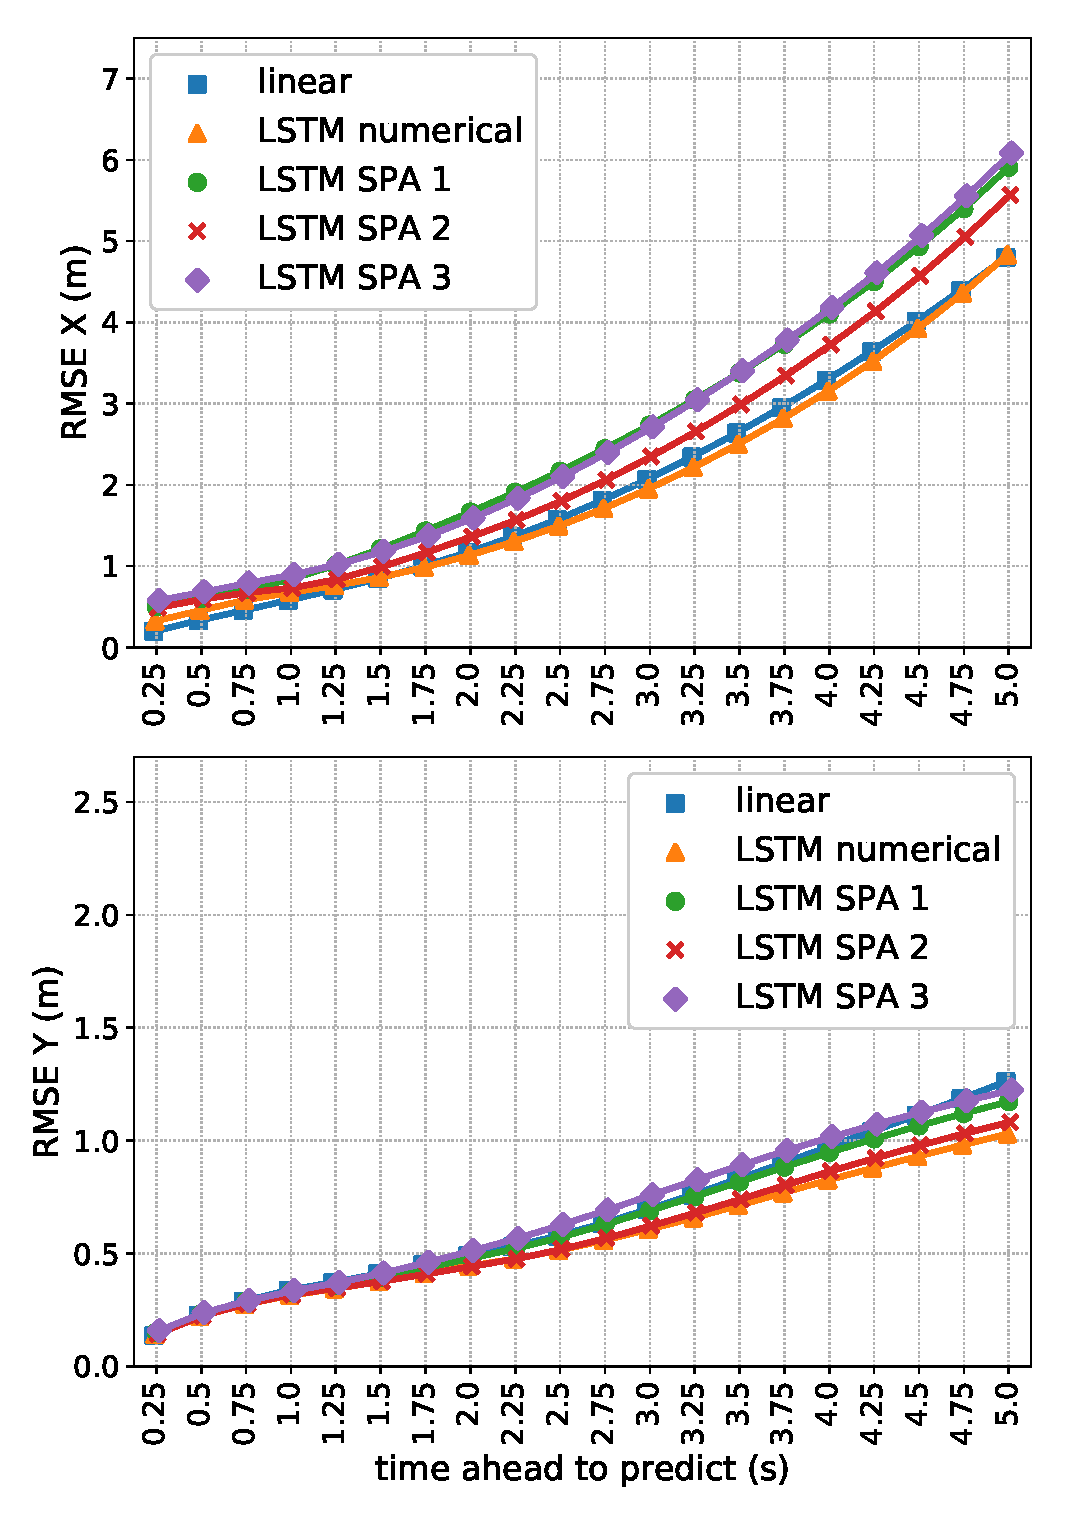
\includegraphics[width=0.25\linewidth]{imgs/rmse_large_all_trained_on_lc.eps}
    }
    %\subfloat[\label{subfig:rmse_large_all_lc_only}Trained on complete data set, evaluated on lane changes samples]{%
    \subfloat[\label{subfig:rmse_large_all_lc_only}]{%
        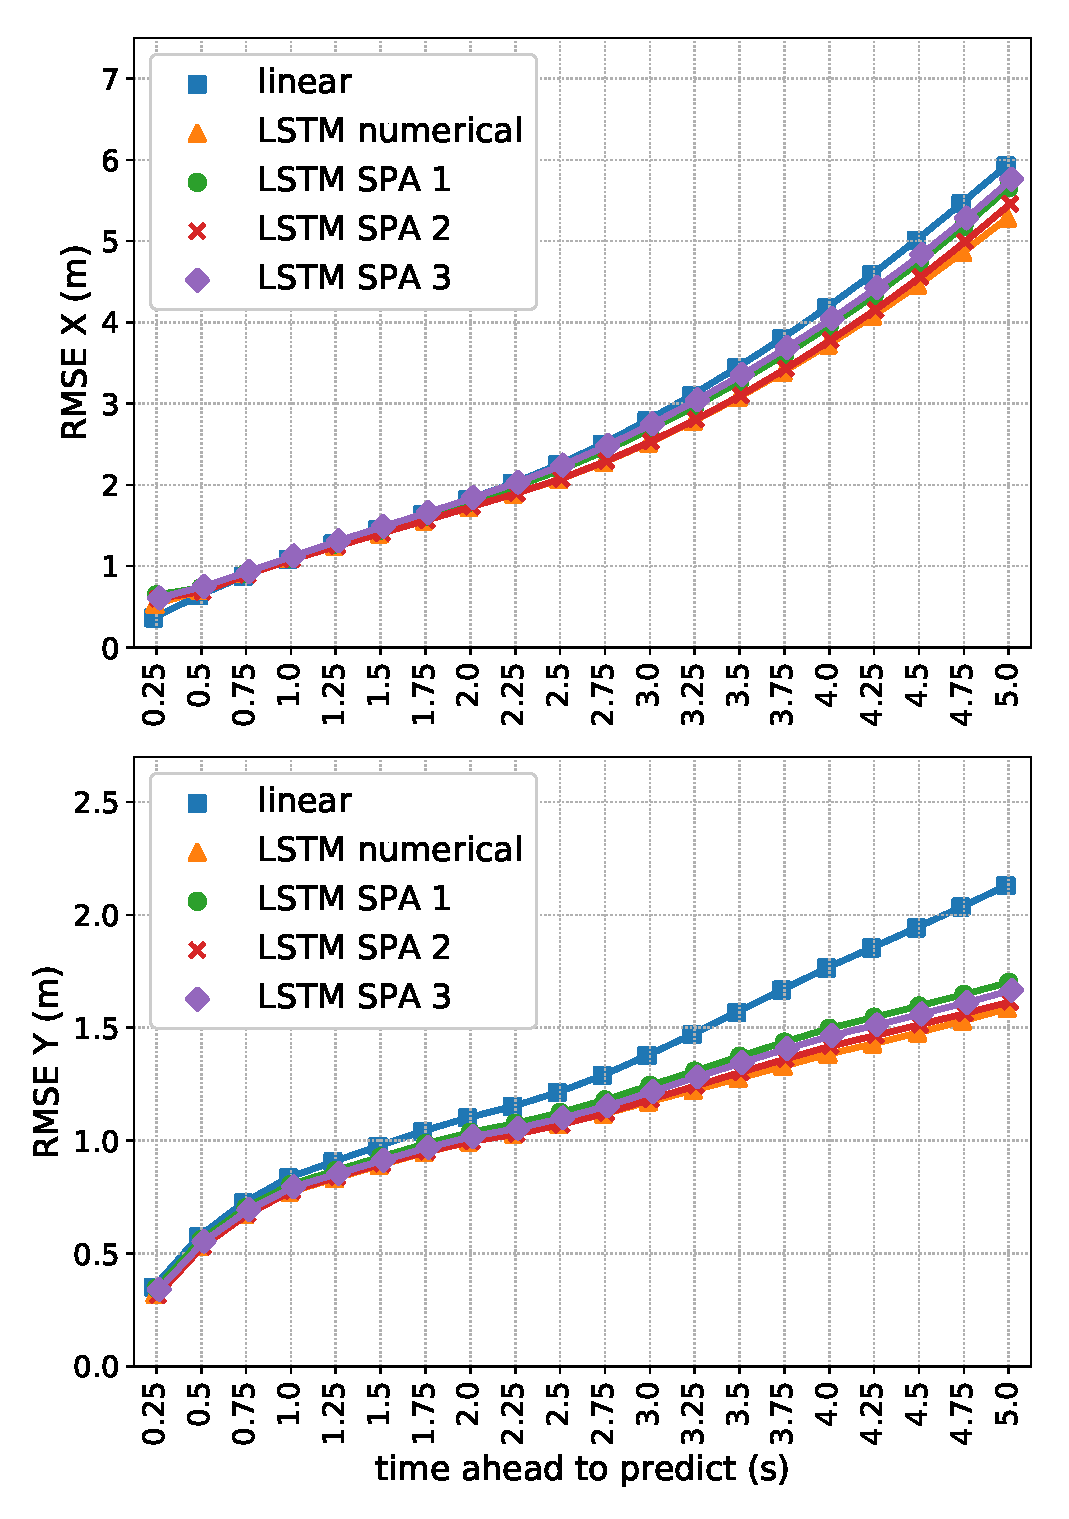
\includegraphics[width=0.25\linewidth]{imgs/rmse_large_all_trained_on_all_evaluated_on_lc.eps}
    }
    %\subfloat[\label{subfig:rmse_large_all_lc_only_trained_on_lc}Trained and evaluated on lane change samples ]{%
    \subfloat[\label{subfig:rmse_large_all_lc_only_trained_on_lc}]{%
        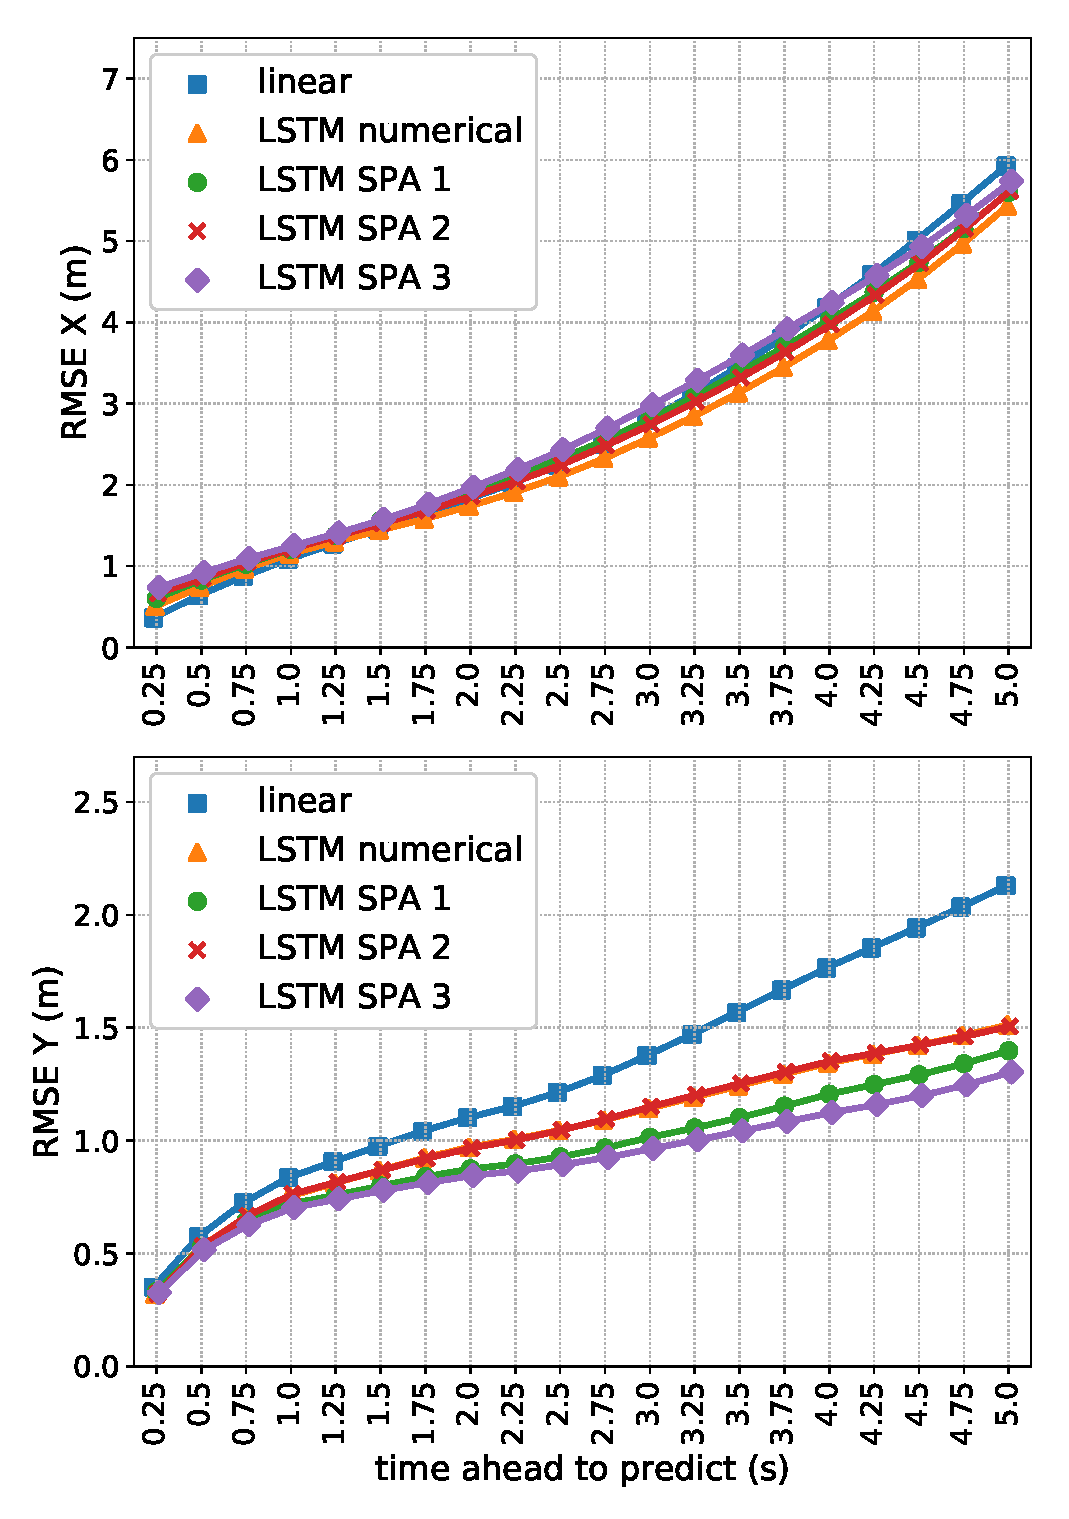
\includegraphics[width=0.25\linewidth]{imgs/rmse_large_all_trained_on_lc_evaluated_on_lc.eps}
    }\\
    %\subfloat[\label{subfig:rmse_large_subset}Trained on complete data set, evaluated on crowded situations]{%
    \subfloat[\label{subfig:rmse_large_subset}]{%
        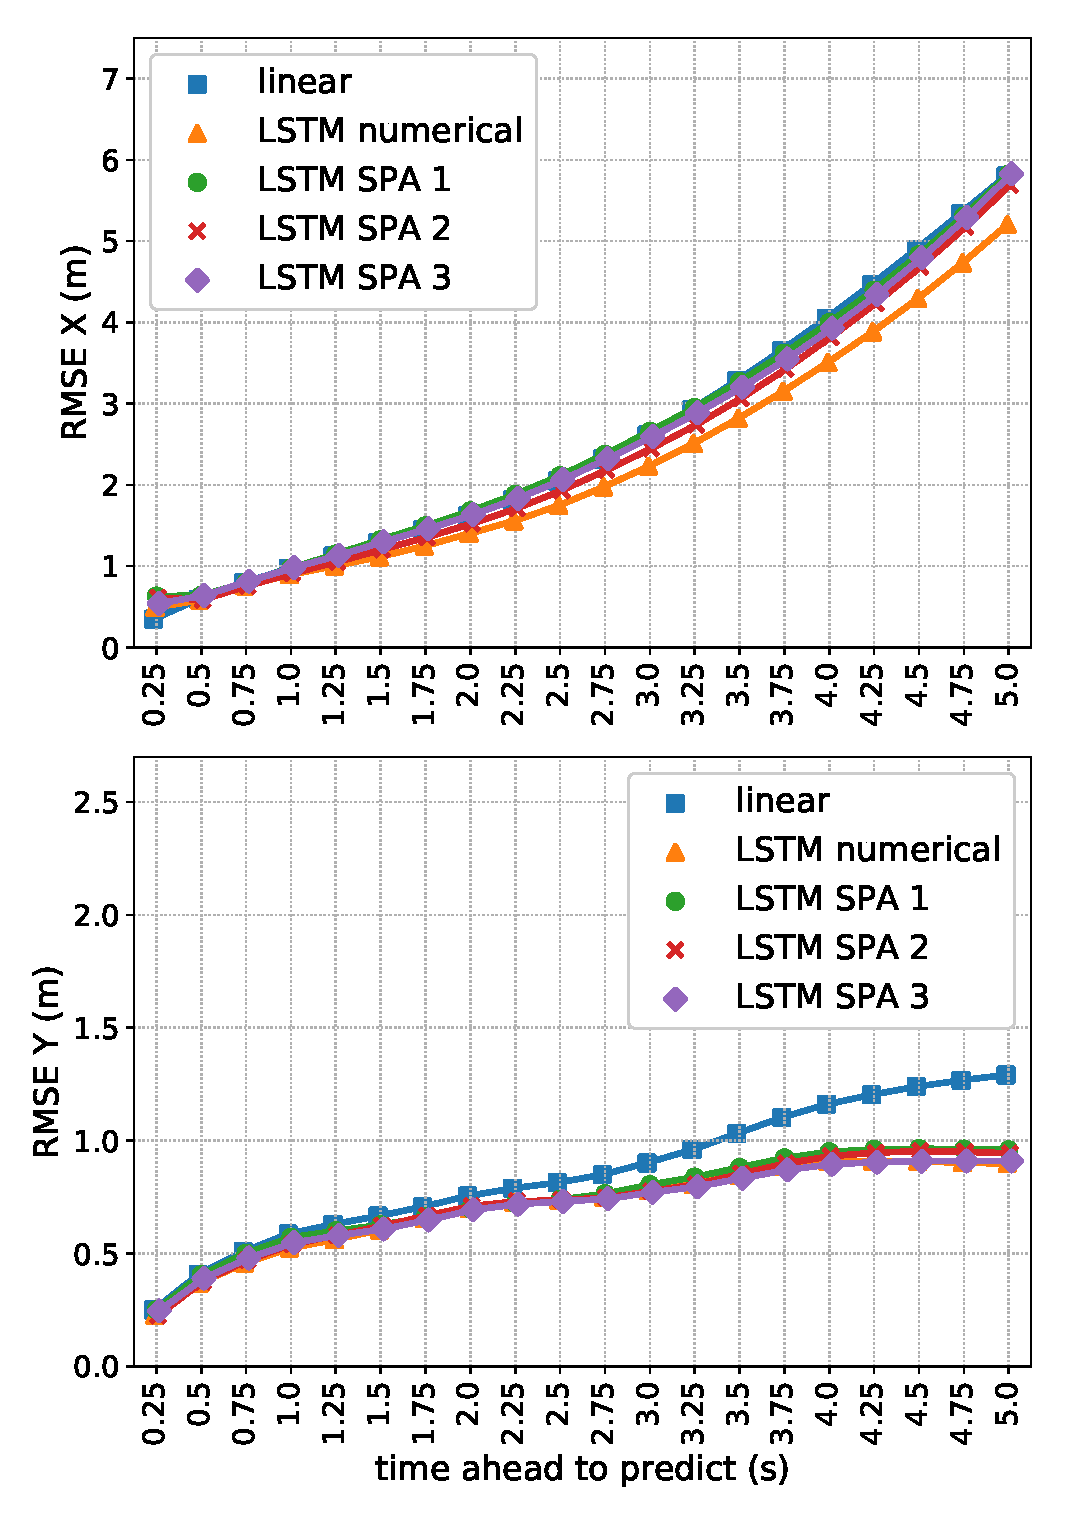
\includegraphics[width=0.25\linewidth]{imgs/rmse_large_subset_trained_on_all.eps}
    }
    %\subfloat[\label{subfig:rmse_large_subset_trained_on_lc}Trained on lane change samples, evaluated on crowded situations]{%
    \subfloat[\label{subfig:rmse_large_subset_trained_on_lc}]{%
        \includegraphics[width=0.25\linewidth]{imgs/rmse_large_subset_trained_on_lc.eps}
    }
    %\subfloat[\label{subfig:rmse_large_subset_lc_only}Trained on complete data set, evaluated on crowded situations with lane changes]{%
    \subfloat[\label{subfig:rmse_large_subset_lc_only}]{%
        \includegraphics[width=0.25\linewidth]{imgs/rmse_large_subset_trained_on_all_evaluated_on_lc.eps}
    }
    %\subfloat[\label{subfig:rmse_large_subset_lc_only_trained_on_lc}Trained on lane change samples, evaluated on crowded situations with lane changes]{%
    \subfloat[\label{subfig:rmse_large_subset_lc_only_trained_on_lc}]{%
        \includegraphics[width=0.25\linewidth]{imgs/rmse_large_subset_trained_on_lc_evaluated_on_lc.eps}
    }
    \caption{Visualization of the \ac{RMSE} performance of our \ac{LSTM} models for different data setups.
    Figures~\protect\subref{subfig:rmse_large_all},~\protect\subref{subfig:rmse_large_all_lc_only},~\protect\subref{subfig:rmse_large_subset} and~\protect\subref{subfig:rmse_large_subset_lc_only} show the \ac{RMSE} for models trained on the complete data set, while
Fig.~\protect\subref{subfig:rmse_large_all_trained_on_lc},~\protect\subref{subfig:rmse_large_all_lc_only_trained_on_lc},~\protect\subref{subfig:rmse_large_subset_trained_on_lc},~\protect\subref{subfig:rmse_large_subset_lc_only_trained_on_lc} show the same models evaluated on the same samples but trained only on the samples including a target vehicle lane change.}
    \label{fig:rmse_on_board_training_data_variation}
\end{figure}


In section~\ref{subsec:data_set_peculiarities}, we have already seen that our prediction models using neural networks have to deal with imbalanced data sets containing significantly more straight driving than lane changes performed by the target vehicle.
Hence, training any learning system on all the samples of both our data sets will expose the system to a significantly higher amount of data, in which most likely already a simple linear prediction model performs reasonably well. 
In this section, we therefore analyze the influence of the training data set on our \ac{LSTM} models and if there are significant differences in the performance of models trained on the complete data sets and on subsets consisting only of such samples that contain a lane change of the target vehicle.
We conduct this analysis on the \emph{On-board} data set only.
Figure~\ref{fig:rmse_on_board_all} showed the performance of our \ac{LSTM}-based models trained on the complete data set.
Here, we train models with the exact same neural network architectures and encoding schemes of the input just on different data sets, namely the subset of samples containing a lane change performed by the target vehicle.
We consider both types of target vehicle lane changes, namely those performed during the trajectory history as well as lane changes performed in the future trajectory to be predicted, as input for the models.
Figure~\ref{fig:rmse_on_board_training_data_variation} shows a comparison of different setups regarding training and evaluation data for our \ac{LSTM}-based trajectory prediction models.
We also keep the simple linear prediction model based on a constant velocity assumption for reference in the figures, since it is not a data-driven learning model and is therefore invariant under the changes of the training data.
Figures~\ref{subfig:rmse_large_all},~\ref{subfig:rmse_large_all_lc_only},~\ref{subfig:rmse_large_subset} and~\ref{subfig:rmse_large_subset_lc_only} show the \ac{RMSE} for models trained on the complete data set while Fig.~\ref{subfig:rmse_large_all_trained_on_lc},~\ref{subfig:rmse_large_all_lc_only_trained_on_lc},~\ref{subfig:rmse_large_subset_trained_on_lc} and~\ref{subfig:rmse_large_subset_lc_only_trained_on_lc} show the same models evaluated on the same samples but trained
only on data samples including a target vehicle lane change.
On the other hand, the upper row of Fig.~\ref{fig:rmse_on_board_training_data_variation}, i.e., Fig.~\ref{subfig:rmse_large_all} -~\ref{subfig:rmse_large_all_lc_only_trained_on_lc}, illustrates the performance of the models evaluated on either the complete data set or only on the lane changes in all data samples, while the lower row of Fig.~\ref{fig:rmse_on_board_training_data_variation}, i.e., Fig.~\ref{subfig:rmse_large_subset} -~\ref{subfig:rmse_large_subset_lc_only_trained_on_lc}, shows the performance
of the models evaluated on samples containing crowded driving situations or crowded situations containing even a target vehicle lane change.

\begin{figure}[t!]
    \centering
    \subfloat[\label{subfig:rmse_large_all_spa_power_trained_on_lc_vs_trained_on_all}All samples]{%
        \includegraphics[width=0.25\linewidth]{imgs/rmse_large_all_spa_power_trained_on_lc_vs_trained_on_all.eps}
    }
    \subfloat[\label{subfig:rmse_large_all_lc_only_spa_power_trained_on_lc_vs_trained_on_all}Lane changes]{%
        \includegraphics[width=0.25\linewidth]{imgs/rmse_large_all_lc_only_spa_power_trained_on_lc_vs_trained_on_all.eps}
    }
    \subfloat[\label{subfig:rmse_large_subset_spa_power_trained_on_lc_vs_trained_on_all}Crowded]{%
        \includegraphics[width=0.25\linewidth]{imgs/rmse_large_subset_spa_power_trained_on_lc_vs_trained_on_all.eps}
    }
    \subfloat[\label{subfig:rmse_large_subset_lc_only_spa_power_trained_on_lc_vs_trained_on_all}Crowded lane changes]{%
        \includegraphics[width=0.25\linewidth]{imgs/rmse_large_subset_lc_only_spa_power_trained_on_lc_vs_trained_on_all.eps}
    }\\
    \subfloat[\label{subfig:rmse_large_all_numerical_trained_on_lc_vs_trained_on_all}All samples]{%
        \includegraphics[width=0.25\linewidth]{imgs/rmse_large_all_numerical_trained_on_lc_vs_trained_on_all.eps}
    }
    \subfloat[\label{subfig:rmse_large_all_lc_only_numerical_trained_on_lc_vs_trained_on_all}Lane changes]{%
        \includegraphics[width=0.25\linewidth]{imgs/rmse_large_all_lc_only_numerical_trained_on_lc_vs_trained_on_all.eps}
    }
    \subfloat[\label{subfig:rmse_large_subset_numerical_trained_on_lc_vs_trained_on_all}Crowded]{%
        \includegraphics[width=0.25\linewidth]{imgs/rmse_large_subset_numerical_trained_on_lc_vs_trained_on_all.eps}
    }
    \subfloat[\label{subfig:rmse_large_subset_lc_only_numerical_trained_on_lc_vs_trained_on_all}Crowded lane changes]{%
        \includegraphics[width=0.25\linewidth]{imgs/rmse_large_subset_lc_only_numerical_trained_on_lc_vs_trained_on_all.eps}
    }
    \caption{Visualization of the changing \ac{RMSE} performance of particular prediction models depending on the data they have been trained on.
        The first four figures~\protect\subref{subfig:rmse_large_all_spa_power_trained_on_lc_vs_trained_on_all} -~\protect\subref{subfig:rmse_large_subset_lc_only_spa_power_trained_on_lc_vs_trained_on_all} illustrate the difference between the \ac{LSTM} \acs{SPA} \num{3} models when changing their training data, while the last four figures~\protect\subref{subfig:rmse_large_all_numerical_trained_on_lc_vs_trained_on_all} -
        ~\protect\subref{subfig:rmse_large_subset_lc_only_numerical_trained_on_lc_vs_trained_on_all} shows the same comparison for the \ac{LSTM} numerical models.
    }
    \label{fig:rmse_on_board_training_all_vs_training_on_lc_only}
\end{figure}

We observe that the models that have been trained only on samples containing a lane change performed by the target vehicle tend to achieve worse results than the models trained on the complete data set, when being evaluated on the entirety of all data samples (Fig.~\ref{subfig:rmse_large_all},,~\ref{subfig:rmse_large_all_lc_only},~\ref{subfig:rmse_large_subset} and~\ref{subfig:rmse_large_subset_lc_only}).
Interestingly, the performance of the models based on the convolutive power encoding scheme (\acs{LSTM} \acs{SPA} \num{1} and \num{3}) deteriorates more significantly compared to the other data-driven models, especially in lateral ($y$) direction.
However, if we evaluate the same models only on the samples containing a target vehicle lane change, their performance changes significantly (Fig.~\ref{subfig:rmse_large_all_trained_on_lc},~\ref{subfig:rmse_large_all_lc_only_trained_on_lc},~\ref{subfig:rmse_large_subset_trained_on_lc},~\ref{subfig:rmse_large_subset_lc_only_trained_on_lc}).
We recapitulate the findings of section~\ref{subsec:data_set_peculiarities} that lane changes influence the lateral ($y$) position values more severely than the longitudinal ($x$) position compared to straight driving samples.
Therefore, the performance difference between the models trained on lane changes only and models trained on the complete data set, as we would expect, is also not that significant in longitudinal direction.
\begin{wraptable}{r}{8cm}
    %\captionof{table}{Summary of the data samples used for the evaluations shown in individual sub-figures of Fig.~\ref{fig:rmse_on_board_training_data_variation}.}
    \resizebox{0.5\textwidth}{!}{%
        \begin{tabular}{|ccc|}
            \hline
            \thead{Setup ID} & \thead{Training set} & \thead{Evaluation set} \\ \hline
            (a) & \makecell{all samples} & \makecell{all samples} \\ \hline
            (b) & \makecell{lane change samples} & \makecell{all samples} \\ \hline
            (c) & \makecell{all samples} & \makecell{lane change samples} \\ \hline
            (d) & \makecell{lane change samples} & \makecell{lane change samples} \\ \hline
            (e) & \makecell{all samples} & \makecell{crowded samples} \\ \hline
            (f) & \makecell{lane change samples} & \makecell{crowded samples} \\ \hline
            (g) & \makecell{all samples} & \makecell{crowded lane change samples} \\ \hline
            (h) & \makecell{lane change samples} & \makecell{crowded lane change samples} \\ \hline
        \end{tabular}
    }
    \caption{Summary of the data samples used for the evaluations shown in individual sub-figures of Fig.~\ref{fig:rmse_on_board_training_data_variation}.}
	\label{tab:eval_setups}
\end{wraptable}
Considering the lateral ($y$) direction however, we observe a significant change between both model and evaluation variants.
If the models are trained only on lane change samples, the \ac{LSTM} \acs{SPA} \num{1} and \num{3} models outperform all other models in lateral direction when evaluated only on the data samples containing a lane change while their performance in longitudinal direction does not change significantly compared to the models trained on the complete data set.

So far, we have only compared either all models trained on the complete data set or all models trained only on the lane change samples.
However, we are also interested in how the performance for particular models changes when modifying the training data set.
Figure~\ref{fig:rmse_on_board_training_all_vs_training_on_lc_only} shows a comparison of the \ac{LSTM}-based models when modifying the training data for the \ac{LSTM} \acs{SPA} \num{3} model (Fig.~\ref{subfig:rmse_large_all_spa_power_trained_on_lc_vs_trained_on_all} -~\ref{subfig:rmse_large_subset_lc_only_spa_power_trained_on_lc_vs_trained_on_all}) as well as the \acs{LSTM} numerical model (Fig.
~\ref{subfig:rmse_large_all_numerical_trained_on_lc_vs_trained_on_all} -~\ref{subfig:rmse_large_subset_lc_only_numerical_trained_on_lc_vs_trained_on_all}).
In this direct comparison, we observe that there is no significant difference in the performance of the numerical \ac{LSTM} models trained on different samples for both evaluation sets containing either the complete data set or only the target vehicle lane changes.
For the \ac{LSTM} \acs{SPA} \num{3} model however, we observe significant improvements for the model trained on the lane change samples when evaluated on the lane changes performed by the target vehicle the model trained on all data samples.
This result indicates that either the numerical model trained on all samples generalizes sufficiently well to all possible situations compared to the convolutive power based model.
However, we have already seen, that both trajectory data sets show a significant imbalance towards straight driving compared to lane change maneuvers (cf.\ section~\ref{subsec:data_set_peculiarities}), which is the same for all models.
On the other hand, the results shown here could also hint, that the convolutive power model encapsulating the prior motion not only of the target vehicle but also other vehicles in its surroundings is better suited to predict lane change maneuvers given a more balanced data set.
These results suggest, that there is not only room for improvement for the models investigated here, but also other data-driven models used for trajectory prediction in the literature, by researching and evaluating the influence of the distribution of driving situations within the training data.

\subsection{Evaluation of \acs{NEF}-based feed-forward prediction models}%
\label{subsec:evaluation_of_nef_based_feed_forward_prediction_models}

In this section, we evaluate the simpler, feed-forward neural networks for trajectory prediction to compare our \ac{LSTM}-based models to.

\subsubsection{Hyperparameter analysis}%
\label{ssubsec:hyperparameter_analysis_nef}

\begin{figure}[t!]
  \centering
  \includegraphics[width=0.95\textwidth]{imgs/nef_num_neurons_analysis.eps}
  \caption{Analysis of the \ac{RMSE} for a varying number of neurons in the learning population of our \ac{NEF} model trained on numerical input from the \emph{On-board} data set.}
  \label{fig:nef_num_neurons_analysis}
\end{figure}

For our \ac{NEF} networks, the main parameter influencing the models' performance is the number of neurons in the learning population, i.e., the hidden layer in terms of traditional neural networks, as well as the neuron model.
For simplicity, we use \acs{Nengo}'s rate-variant of the \ac{LIF} neuron model.
Here, we inspect the number of neurons in the learning population in more detail.
From the \ac{NEF}-theory \parencite{Eliasmith2003} we know that increasing the number of neurons in a population yields a more accurate representation of the data encoded in the population's activity.
Thus, we expect more accurate predictions when increasing the number of neurons.
Figure~\ref{fig:nef_num_neurons_analysis} shows the \ac{RMSE} of different model instantiations with varying number of neurons, namely \num{1000}, \num{3000}, \num{5000} and \num{8000} neurons.
We observe that a number of \num{3000} spiking neurons is sufficient and further increasing the number of neurons does not improve the model's prediction accuracy.
Note that the order of magnitude of the \ac{RMSE} in Fig.~\ref{fig:nef_num_neurons_analysis} is significantly higher than for the figures visualizing the \ac{LSTM} models \ac{RMSE} inspected in the previous section. 
This is due to the fact that the \ac{NEF} models investigated here receive less amount of information, namely only position data and instantaneous velocity of the target vehicle, compared to the \ac{LSTM} models.
Here, we are only interested to find the best possible parameter setup, whereas we will evaluate both models with comparable setups in later sections.

\subsubsection{Model training}%
\label{ssubsec:model_training_nef}

We train two different variants of our simpler \ac{NEF}-models using numerical input (\acs{NEF} numerical) as well as the \ac{SPA}-power-with-ego (\acs{NEF} \acs{SPA} \num{1}) and \ac{SPA}-power encoding (\acs{NEF} \acs{SPA} \num{2}) for the \emph{On-board} and the \emph{\ac{NGSIM}} data set respectively.
The neural weights are calculated using \acs{Nengo}'s default least-squares-optimization method with the exception, that we calculate the weights over smaller subsets of the input data for computational reasons.
Here, we adapt the input data such that for the numerical \ac{NEF}-model, we use the vector $(x_{t_{0}}, \ldots, x_{t_{N}}, y_{t_{0}}, \ldots, y_{t_{N}}, v)$ as input with $v$ denoting the instantaneous velocity of the target vehicle.
For the \ac{SPA}-power encoding schemes, instead of flattening the whole sequence of vectors into one giant single vector, we created a single semantic vector by summing the first, middle and last element of the original vector sequences

\begin{figure}[t!]
	\centering
    \subfloat[\label{subfig:nef_rmse_512_onboard}]{%
        \includegraphics[width=0.5\columnwidth]{imgs/rmse_on_board_nef_nets.eps}
    }
    \subfloat[\label{subfig:nef_rmse_1024_ngsim}]{%
        \includegraphics[width=0.5\columnwidth]{imgs/rmse_ngsim_nef_nets.eps}
    }
    \caption{Visualization of the \ac{RMSE} of all \ac{NEF}-network models~\protect\subref{subfig:nef_rmse_512_onboard} on the \emph{On-board} validation set $V_1 \subset D_1$ using \num{512}-dimensional vectors for the \ac{SPA}-power vectors and~\protect\subref{subfig:nef_rmse_1024_ngsim} on the \emph{\ac{NGSIM}} data set $D_2$ using \num{1024}-dimensional vectors for the \ac{SPA}-power vectors.}\label{fig:rmse_nef_nets}

\end{figure}

\begin{equation}
  \hat{\mathbf{S}} =  \mathbf{S}_{t_0} \oplus \mathbf{S}_{t_{\nicefrac{N}{2}}} \oplus \mathbf{S}_{t_N} = (\hat{s}_0, \ldots, \hat{s}_{D-1}).
\end{equation}
We only sum up these vectors instead of the whole sequence $(\mathbf{S}_{t})_{t_0}^{t_N}$ to avoid the accumulation of noise in the vector representation.
Note that thereby the \ac{NEF} model using the \ac{SPA}-power representation does not use the full trajectory history but only selected time steps, namely those visualized in Fig.~\ref{fig:spa_power}.
We also include the instantaneous velocity $v$ of the target vehicle as an additional vector element, which yields $(\hat{s}_0, \ldots, \hat{s}_{D-1}, v)$ as input of our model.
To make these simpler models as comparable as possible to the \ac{LSTM} models in terms of information available to the network, we add the instantaneously velocity of the target vehicle as an additional element to the input, since there is no intermediate embedding vector here where it could be included.

\subsubsection{Evaluation}%
\label{ssubsec:evaluation_nef}

Figure~\ref{fig:rmse_nef_nets} visualizes the \ac{RMSE} of our \ac{NEF}-network models on both data sets.
The \ac{NEF}-network using the \ac{SPA}-power encoding schemes processes \num{512}-dimensional for the \emph{On-board} (\ac{NEF} \ac{SPA} \num{1}) and \num{1024}-dimensional vectors for the \emph{\ac{NGSIM}} data set (\ac{NEF} \ac{SPA} \num{2}).
For reference, we included the performance of the most relevant \ac{LSTM} models, namely \ac{LSTM} \ac{SPA} \num{1} and \num{3} for the \emph{\ac{NGSIM}} and \emph{On-board} data set respectively as well as \ac{LSTM} numerical, in Fig.~\ref{fig:rmse_nef_nets} as well.
We observe that, despite a simpler network architecture and learning algorithm, the \ac{NEF}-networks achieve a performance comparable to the more sophisticated \ac{LSTM} models on both data sets.
For the \emph{\ac{NGSIM}} data set, the \ac{NEF} \ac{SPA} \num{1} model performs on par with its \ac{LSTM} model counterpart \ac{LSTM} \ac{SPA} \num{3}.
In this case, the \ac{NEF}-model is not only simpler, but also has access to less information as its input data is a sum of a subset of the input sequence used for the corresponding \ac{LSTM}-model.

\subsection{Evaluation of the unsupervised anomaly detection}%
\label{subsec:evaluation_of_the_unsupervised_anomaly_detection}

\begin{figure}[t]
	\centering
	\resizebox{.8\textwidth}{!}{%
	\begin{tikzpicture}[%
	auto,
	multilayer,
	]
    \Vertices{data/autoenc_vertices.csv}
    \Edges{data/autoenc_edges.csv}
    \draw (-4.0,-1.6)--(-4.0,-1.6) node[below, text width=2.5cm]{input \\layer};
    \draw (-3.0,0.5)--(-3.0,0.5) node[below, text width=2.5cm]{enc layer \num{1}\\ \num{64} neurons};
    \draw (-2.0,3)--(-2.0,3) node[below, text width=2.5cm]{enc layer \num{2}\\ \num{32} neurons};
    \draw (-2.0,5.5)--(-2.0,5.5) node[below, text width=2.5cm]{dec layer \num{1}\\ \num{32} neurons};
    \draw (-3.0,8)--(-3.0,8) node[below, text width=2.5cm]{dec layer \num{2}\\ \num{64} neurons};
    \draw (-4.0,10.5)--(-4.0,10.5) node[below, text width=2.5cm]{reconstruct\\layer};
    \draw (-4.0,-1.6)--(-4.0,-1.6) node[below, text width=2.5cm]{input \\layer};
    \end{tikzpicture}
	}
    \caption{A schematic visualization of our autoencoder neural network architecture.} 
    \label{fig:autoenc_arch}
\end{figure}

In this section, we analyze and evaluate the results of the performance of the anomaly detection network introduced in section~\ref{subsec:excursion_on_unsupervised_anomaly_detection}.
We train a fully-connected autoencoder neural network with \num{4} hidden layers consisting of \num{64}, \num{32}, \num{32} and \num{64} neurons in unsupervised fashion to generate replicates of the original vectors used as input to the network.
Figure~\ref{fig:autoenc_arch} shows a schematic visualization of the network's architecture.
We use the reconstruction error between the original vectors and the replicates generated by the neural network as anomaly score and calculate a threshold for the error to detect outliers based on the percentage of anomalies we expect in the data set.
For this evaluation, we use \SI{10}{\percent} for the amount of expected outliers within the data set and trained the network for \num{100} epochs on the vectors encoding the current scene using the convolutive power representation as described in section~\ref{ssubsec:convolutive_power_representation}.

\begin{figure}[t]
    \centering
    \subfloat[\label{subfig:anomalies_on_board_boxplots_distances}]{%
        \includegraphics[width=0.5\linewidth]{imgs/anomalies_on_board_boxplots_distances.eps}
    }
    \subfloat[\label{subfig:anomalies_on_board_boxplots_other_vehicles}]{%
        \includegraphics[width=0.5\linewidth]{imgs/anomalies_on_board_boxplots_other_vehicles.eps}
    }\\
    \subfloat[\label{subfig:anomalies_on_board_histograms_distances}]{%
        \includegraphics[width=0.5\linewidth]{imgs/anomalies_on_board_histograms_distances.eps}
    }
    \subfloat[\label{subfig:anomalies_on_board_histograms_other_vehicles}]{%
        \includegraphics[width=0.5\linewidth]{imgs/anomalies_on_board_histograms_other_vehicles.eps}
    }
    \caption{Visualization of the results of the autoencoder neural network used for unsupervised anomaly detection on the \emph{On-board} data set.
        The figures show the distribution of certain characteristic values, namely distances between the target and other vehicles (Fig.~\protect\subref{subfig:anomalies_on_board_boxplots_distances} and~\protect\subref{subfig:anomalies_on_board_histograms_distances}) as well as the number of other vehicles (Fig.~\protect\subref{subfig:anomalies_on_board_boxplots_other_vehicles} and~\protect\subref{subfig:anomalies_on_board_histograms_other_vehicles}), for situations classified as anomalies and for the complete data set.
        The upper row shows box plots to visualize the difference between anomalies and the complete data set, whereas the lower row shows histograms for a more in-depth visualization of the metrics' distribution.
}
    \label{fig:anomaly_on_board}
\end{figure}

Since the data we are using to train the network is unlabeled, i.e., we do not have any information available which vectors belong to unusual or atypical situations, we have no way of comparing the results produced by the neural network with actual ground truth data.
Hence, our only option is to analyze the anomalies detected by our neural network with respect to certain characteristic values describing the driving situation and compare them to the values of the complete data set.
If this comparison uncovers significant differences between the anomalies detected by the neural network and the entirety of all data samples, we can at least conclude that the anomalies are reasonably different from the rest of the data set and furthermore, that there is sufficient information encoded in our vector representation to unravel them.
For this analysis, we use the same metrics already analyzed in section~\ref{ssubsec:evaluation_nef} to characterize crowded and potentially dangerous driving situations, namely the distance between the target and the ego-vehicle, the distance between the target and the closest other vehicle and the number of other vehicles present in the scene.
Figure~\ref{fig:anomaly_on_board} visualizes the distribution of these metrics on the set of anomalies produced by the neural network and on all data samples in the \emph{On-board} data set.
Figure~\ref{subfig:anomalies_on_board_boxplots_distances} shows box plots of the distances between the target and the closest other vehicle (left plot in Fig.~\ref{subfig:anomalies_on_board_boxplots_distances}) as well the target and the closest other vehicle (right plot in Fig.~\ref{subfig:anomalies_on_board_boxplots_distances}) while Fig.~\ref{subfig:anomalies_on_board_histograms_distances} shows the same data, but illustrated as histograms.
Figure~\ref{subfig:anomalies_on_board_boxplots_other_vehicles} and~\ref{subfig:anomalies_on_board_histograms_other_vehicles} visualize a similar evaluation for the number of other vehicles within a certain distance (left plots), namely \SI{40}{\meter}, and all other vehicles in the scene (right plots).

\begin{figure}[t]
    \centering
    \resizebox{.9\textwidth}{!}{%
        \subfloat[\label{subfig:anomalies_ngsim_boxplot_distance}]{%
            \includegraphics[height=3cm]{imgs/anomalies_ngsim_boxplot_distance.eps}
        }
        \subfloat[\label{subfig:anomalies_ngsim_histogram_distance}]{%
            \includegraphics[height=3cm]{imgs/anomalies_ngsim_histogram_distance.eps}
        }
    }\\
    \resizebox{.9\textwidth}{!}{%
        \subfloat[\label{subfig:anomalies_ngsim_boxplot_other_vehicles}]{%
            \includegraphics[height=3cm]{imgs/anomalies_ngsim_boxplot_other_vehicles.eps}
        }
        \subfloat[\label{subfig:anomalies_ngsim_histogram_other_vehicles}]{%
            \includegraphics[height=3cm]{imgs/anomalies_ngsim_histogram_other_vehicles.eps}
        }
    }
    \caption{Visualization of the results of the autoencoder neural network used for unsupervised anomaly detection on the \emph{\ac{NGSIM}} data set.
        The figures show the distribution of distances between the target and other vehicles (Fig.~\protect\subref{subfig:anomalies_ngsim_boxplot_distance} and~\protect\subref{subfig:anomalies_ngsim_histogram_other_vehicles}) as well as the number of other vehicles (Fig.~\protect\subref{subfig:anomalies_ngsim_boxplot_other_vehicles} and~\protect\subref{subfig:anomalies_ngsim_histogram_other_vehicles}), for situations classified as anomalies and for the complete data set.
    The left figures (Fig.~\protect\subref{subfig:anomalies_ngsim_boxplot_distance} and~\protect\subref{subfig:anomalies_ngsim_boxplot_other_vehicles}) show box plots to visualize the difference between anomalies and the complete data set, whereas the right figures (Fig.~\protect\subref{subfig:anomalies_ngsim_histogram_distance} and~\protect\subref{subfig:anomalies_ngsim_histogram_other_vehicles}) show histograms for a more in-depth visualization of the metrics' distribution.}
    \label{fig:anomaly_ngsim}
\end{figure}

We observe a clear difference for both, the evaluation of the distances and the number of other vehicles, between the anomalies detected by our neural network and the complete set of data samples.
Focusing on the distance information, the number of instances with smaller distances between the ego-vehicle or the closest other vehicle and the target is significantly higher for the anomalies than for the complete data set.
While the mean distance between the target and closest other vehicle is slightly below \SI{20}{\meter} for the complete data set, the mean distance for the anomalies is \SI{10}{\meter} (cf.\ Fig.~\ref{subfig:anomalies_on_board_boxplots_distances}) with clear concentration below \SIrange{0}{15}{\meter} (cf.\ Fig.~\ref{subfig:anomalies_on_board_histograms_distances}).
We observe a similar distribution for the distance between the target and the ego-vehicle, where the distances are more or less equally distributed around the mean of \SI{40}{\meter} for the complete data set.
For the anomalies, we observe a concentration of the distances between the target and the ego-vehicle below \SI{40}{\meter} around the mean of \SI{25}{\meter}.
Regarding the number of other vehicles, the difference between the complete data set and the anomalies detected by our neural network is even clearer.
For the complete data set, the mean number of other vehicles within \SI{40}{\meter} to the target vehicle is \num{2}, while the total mean number of other vehicles is around \num{4}.
Both numbers are significantly higher for the anomalies with a mean number of \num{5} other vehicles within \SI{40}{\meter} and a mean of \num{7} other vehicles in total (cf.\ Fig.~\ref{subfig:anomalies_on_board_boxplots_other_vehicles}).
Looking at the distribution shown in the histograms in Fig.~\ref{subfig:anomalies_on_board_histograms_other_vehicles}, the picture becomes even clearer. 
There are no situations with less then \num{3} other vehicles within \SI{40}{\meter} to the target vehicle in the set of anomalies, whereas in this same range fall the majority of samples of the complete data set.
We observe a similar distribution for the total number of other vehicles in the scene with the anomaly samples having at least \num{3} and the majority of examples having at least \num{4} other vehicles present in the scene.
In contrast, the great majority of samples from the complete data set has at most \num{7} other vehicles present and the overall distribution is somewhat inverse to that of the anomalies.

Figure~\ref{fig:anomaly_ngsim} shows a similar analysis for the \emph{\ac{NGSIM}} data set with a few systematic differences.
Since the \emph{\ac{NGSIM}} data set is recorded with external cameras observing highway traffic, there is no ego-vehicle to evaluate regarding the distance to the target vehicle.
Hence, we only analyze the distance between the target vehicle and the closest other vehicle (see Fig.~\ref{subfig:anomalies_ngsim_boxplot_distance} and~\ref{subfig:anomalies_ngsim_histogram_distance}).
Furthermore, since the external cameras record highway traffic on \num{6} lanes on a segment of \SI{640}{\meter} length for the \emph{\ac{NGSIM}} data set, we needed to reduce the number of vehicles to be included in our vector representation to the ones most relevant for the prediction task.
Therefore, we focus on vehicles within a distance of \SI{40}{\meter} on lanes adjacent to the target vehicle's lane for the analysis of our anomaly detection network here as well (see Fig.~\ref{subfig:anomalies_ngsim_boxplot_other_vehicles} and~\ref{subfig:anomalies_ngsim_histogram_other_vehicles}).
While the differences between anomalies and the complete data set regarding the distance between the target and the closest other vehicle is not as significant for the \emph{\ac{NGSIM}} data set in comparison to the \emph{On-board} data set, we still observe a similar tendency for the anomalies to capture situations with smaller distances between the target and the closest other vehicle.
For the number of other vehicles however, we also observe that the samples detected as anomalies by our autoencoder network tend to have more vehicles in the target vehicle's surroundings present than for all the samples within the \emph{\ac{NGSIM}} data set.

In conclusion, our autoencoder neural network is able to detect a subset of anomalies consistently for both, the \emph{On-board} and \emph{\ac{NGSIM}} data set, which show sufficiently significant differences to the complete data set regarding certain metrics.
The results indicate, that the anomalies detected by the network have a tendency towards crowded situations with rather small distances between the target vehicle and the other vehicles in its surroundings.
Since these are the kind of situations, where our prediction models based on the \ac{SPA}-based convolutive power encoding tend to perform better than the other reference models, these results offer interesting directions for future research.
For instance, we could combine the anomaly detection network based on our vector representation presented in this section with the behavior prediction networks to decide whether the current driving situation is potentially hazardous and needs more accurate predictions than less crowded or dangerous situations. 
We have already seen in section~\ref{subsec:evaluation_of_the_lstm_based_prediction_models}, that the \ac{LSTM} models employing the convolutive power representation (\ac{LSTM} \ac{SPA} \num{1} and \num{3}) outperform the other models in such situations particularly in lateral direction. 
Furthermore, one could also imagine to let the outlier detection network guide the training process of the behavior prediction networks.
That is, we could train prediction models particularly on lane changes, the outliers and a similar amount of \enquote{normal} samples to create a more balanced training data set.
We have already seen that the networks using semantic vectors benefit from a more focused and specific training data set, since the models trained particularly on lane changes improved especially in lane change situations compared to network variants trained on all samples.
Finally, we could also investigate other anomaly detection algorithms in addition to the autoencoder models shown here to get a better idea what sort of data samples are actually  outliers by evaluating how different models classify anomalies differently.

\section{Summary}%
\label{sec:summary_behavior_prediction}

In this chapter, we showed a novel approach to encapsulate spatial information of multiple objects in a sequence of semantic pointers of fixed vector length.
We used a \ac{LSTM} sequence to sequence model as well as a simple feed-forward \acl{SNN} to predict future vehicle positions from this representation.
For each of those models, we implemented at least one reference model using other encoding schemes to compare their performance to.
Furthermore, we compared all our models to a simple linear predictor based on a constant velocity assumption.
We evaluated our models on two different data sets, one recorded with on-board sensors from a driving vehicle and one publicly available trajectory data set recorded with an external camera observing a highway segment and conducted a thorough analysis.

For the trained neural networks, simple feed-forward \ac{NEF} models and more sophisticated \ac{LSTM} models alike, we observe that most improvements over the linear model are achieved in $y$-direction.
That makes sense as linear prediction is unable to account for lane-changes or driving curves, which are mainly characterized by non-linear changes in $y$-direction.
We found that the \ac{LSTM} models based on our \ac{SPA}-power representation achieve promising results on both data sets.
However, for the \emph{On-board} data set, this encoding scheme achieves its best result in crowded and potentially dangerous driving situations, without clearly outperforming the other approaches on the whole data set (see section~\ref{subsec:evaluation_of_the_lstm_based_prediction_models} and Fig.~\ref{fig:rmse_on_board_all}).
Given these finding, we investigated situations, where the \ac{SPA}-power representation does outperform all other approaches in $y$-direction and thereby came up with metrics characterizing such crowded situations (see Fig. \ref{fig:histograms_on_board}).
This result did not hold that clearly on the \emph{\ac{NGSIM}} data set $D_2$, since the \ac{LSTM} models achieve an almost identical performance in $y$-direction on this data set.
On the other hand, employing an unsupervised learning method for anomaly detection yielded a significantly higher amount of such crowded situations within the samples classified as anomalies compared to the normal samples.
Additionally, we found that when training the \ac{LSTM} models only on data samples containing a lane change performed by the target vehicle, that the model employing the \ac{SPA}-power representation clearly outperforms all other approaches in $y$-direction when evaluated on the samples containing a lane change.
These results suggest that training the whole system on a more balanced data set containing equally many lane change and straight driving samples could improve overall model performance.

Another interesting result of our experiments is the fact that the simple, feed-forward \ac{NEF} networks show results comparable to the more sophisticated \ac{LSTM} models.
For those simple models, the \ac{SPA}-power representation shows promising results comparable to the \ac{NEF} model using numerical input on the \emph{On-board} data set and clearly outperforming it on the \emph{\ac{NGSIM}} data set (Fig. \ref{fig:rmse_nef_nets}).
Although the \ac{NEF} models do not clearly outperform the \ac{LSTM} models (which would be surprising), it is quite remarkable that they achieve results comparable to the more sophisticated models with a simpler network architecture, training procedure and, partly, less information.
These results make those simple models using our proposed vector-representation as well as a numerical encoding scheme (possibly in combination with an online learning system like the one proposed in chapter~\ref{chap:mix_online_learning}) potential candidates to be deployed on dedicated neuromorphic hardware in mobile applications, as they can be efficiently implemented in a spiking neuron substrate.
This could be an interesting, power-efficient approach in future automated vehicles.

Finally, given the results that there is not one model clearly outperforming all the others in all evaluated situations, we aim to implement an online model meant to be trained at run time to weight the predictions of several models, which have been trained offline, to improve over the individual predictors.
We will introduce and evaluate such a model in the next chapter.

\chapter{A mixture of experts online learning system}
\label{chap:mix_online_learning}

In this chapter, we continue our work on behavior prediction from chapter ~\ref{chap:behav_pred}.
Although the various models developed there show already promising results, they are intended to be trained offline and without any adaptation at run time.
Furthermore, our analysis has shown, that each of the developed models has its own strengths and weaknesses in particular driving situations or even perform differently regarding the direction of motion.
Hence, relying on just one specific predictor would lead to sub-optimal performance in situations where one of the other models is superior.
Therefore, we implement mixture-of-experts models, that choose at run time between several available prediction models.
Thereby, we tackle the aforementioned issues with only one prediction model that has been trained offline, i.e.\ before deployment.
By training a model at run time, we expect improved performance of the mixture model over the individual input predictors.
One option for investigating such an online learning system is the information based on which the model optimizes its weights.
In its simplest form, the model adjusts its weight only based on the prediction error, i.e.\ the difference between its prediction and the actual motion of the target vehicle.
However, we have seen in sec. ~\ref{subsec:eval_behav_pred} that the performance of the individual models heavily depend on the current driving situation.
Therefore, we also investigate online learning models, that adjust their predictions based on some sort of contextual information.
We use the findings from sec. ~\ref{subsec:eval_behav_pred} as a first hint regarding potential context information.\\  
However, there are several potential problems with such an online learning approach: we need to make sure, that the model trained online actually yields improvements without ruining the performance.
Furthermore, as the actual motion of the predicted vehicle is not available at the moment when the prediction needs to happen.
Therefore, we need to find a mechanism to propagate the error between the actual motion of the target vehicle and the model's prediction back in time to update the weights correctly.
%This could yield to poor model adaptation whil

\section{Instantiating a context-free online learning model}
\label{sec:context_free_online}

Given that we have multiple models for predicting vehicle positions, we define our mixture-of-experts model in the following way.
The output of our model is a weighted sum of the outputs from the other  models.
Let us assume we have $M$ different models for vehicle prediction and let $p_i$ for $i=1, \ldots, M$ be the predictions of these models.
Then the output of our mixture-of-experts model will be,
\begin{equation}
    p_{mixture} = \sum_{i=1}^{M} w_i p_i,
    \label{eq:mixture_of_experts}
\end{equation}
where $w_i$ is the weight associated with the prediction of the $i$th model.
As each model produces a prediction of the $x$ and $y$ positions at $N$ different time steps into the future and we have $M$ models, $w$ will be an $M \times N \times 2$ tensor.
In other words, the particular weighting of models for predicting 0.5 seconds into the future may be very different from the weighting when predicting 5.0 seconds into the future.\\
The simplest way to generate these weights is to use standard delta-rule learning
\begin{equation}
	\label{eq:delta_rule}
    \Delta w_i = \kappa p_i \epsilon
\end{equation}
where $\kappa$ is a learning rate and $\epsilon = p_{actual} - p_{mixture}$ is the current prediction error.
Here, we initialize the weights $w_i$ to be $1/M$, i.e.\ an equal weighting across all $M$ models.

\section{Instantiating a context-sensitive online learning}
\label{sec:context_sensitive_online}
The above model attempts to find the best weighting of the base models based only on the prediction error.
However, it is also possible to learn a weighting that is based on the current \textit{context}.
That is, instead of learning $w$, we can learn the function $f_w(c)=w$, where $c$ is some currently available sensor information.

Since neural networks are good function approximators, we implement this context-sensitive mixture-of-experts model as a single-hidden-layer \ac{ANN} whose inputs are $c$ and whose outputs are $w$.
As with the context-free mixture-of-experts model, we initialize the output to always produce $1/M$, and then train the network based on the prediction error.

Importantly, this context-sensitive mixture-of-experts model is meant to be trained \textit{online}.
That is, we do not pre-train it on a large corpus of data and then fix the final weights.  Instead, we run the neural network training \textit{while the system is running}, just like the context-free version.
Indeed, the context-free version is equivalent to the context-sensitive model if the context is kept constant.

While any neural network learning algorithm could be used here, for simplicity we use delta rule again, and note that the delta rule is the first step of the classic backpropagation neural network learning algorithm.
In other words, we just adjust the weights between the hidden layer and the output layer, and leave the other set of weights at their initial randomly generated values.
This greatly reduces the computation cost of performing the online learning.
\begin{figure}[t!]
    \centering
    \includegraphics[width=\textwidth]{imgs/mix_of_experts.eps}
    \caption{Visualization of the network architecture of the context-sensitive mixture-of-experts online learning system. The red arrow indicates the learning connection, whereas the dotted green arrow indicates that the error signal is used to updated the weights of this connection using delta-rule learning.}\label{fig:data_example}
\end{figure}

There are two different possible variants to our mixture-of-experts online learning model.
One issue of such a learning system is that the actual position information of the target vehicle $p_{actual}$ and thus the error $\epsilon$ in eq.~\ref{eq:mixture_of_experts} is not available instantaneously but timely delayed.
Here, we show a first prototype that, for simplicity, ignores this delay issue and assumes that position information of the target vehicle $p_{actual}$ actually is available at prediction time.
In the future, we aim to investigate an online learning system that updates its weights $w_i$ once the error signal $\epsilon$ gradually becomes available.
However, the architecture of the model itself remains the same.
The only difference to the prototype shown here is the time when eq.~\ref{eq:mixture_of_experts} is applied to update the neural weights.
For the context-sensitive mixture-of-experts model, we use information about the current driving situation as identified in Sec.~\ref{subsubsec:eval_lstm} and Fig.~\ref{fig:histograms_on_board} as context $c$ for the learning system.
For the \emph{\ac{NGSIM}} data-set, we use the distance between the target-vehicle and the closest other vehicle as well as the number of surrounding relevant vehicles as context information.
Relevant means that those vehicles that are included in the \ac{SPA}-power representation are counted (see Sec.~\ref{subsubsec:encoding_schemes}).
For the \emph{On-board} data-set, the distance between the target and the ego-vehicle is additionally included in the context.

In this work, we employ the pre-trained \ac{LSTM} models using numerical inputs, the best-performing \ac{SPA}-power encoding scheme for each data-set, and a simple linear prediction as experts for our online learning prototype.
For training the model, we simulate online deployment by presenting the \ac{LSTM} models' predictions on the validation subsets to the system.
Thereby, the individual experts perform their prediction on previously unseen data samples.
We conduct individual simulation runs for each of both data-sets.

\section{Summary}
\label{sec:online_learn_summ}


\chapter{Closed-loop neuromorphic control systems}%
\label{chap:closed_loop_neuromorphic_control_systems}

In this chapter, we present a first step towards a neuromorphic control architecture, that can be used to implement generic control algorithms in the language of \acfp{SNN}.
This offers the advantage that the overall task can be divided into several sub-networks.
We develop two sample instantiations of neurally-inspired control algorithms, namely for mobile robot manipulation and vehicle trajectory control based on reinforcement learning.
Here, we partly depart from the application of automated driving using real-world data, which is an intentional choice.
As mentioned earlier, control of an automated vehicle is an extremely safety-critical task.
Furthermore, current vehicle hardware architectures are designed neither to include neuromorphic hardware nor to efficiently process \acp{SNN}.
Therefore, we demonstrate the general feasibility of this neuromorphic control architecture on the task of bringing order in a sequence of unordered visual stimuli detected using a neuromorphic vision sensor, the \ac{DVS} (section~\ref{sec:sensorimotor_adaptation_for_mobile_robotic_manipulation}). 
The second demonstration scenario is closer to automotive context, presenting a system employing reinforcement learning for short-term vehicle trajectory planning evaluated in the simulated environment of \acf{TORCS} \parencite{TORCS}.
Both applications demonstrate certain aspects of the control architecture: the mobile manipulation tasks shows how the principles of neural engineering can be used to manually program non-trivial tasks in a spiking neural substrate.
This can be useful, to either bootstrap learning to improve task performance without having to start the process from an initial blank state or to complement learning networks with manually designed networks involving human expert knowledge.
The second task presents such a combination in an instantiation of the neuromorphic control architecture, with a trajectory selection module employing reinforcement learning while all other modules are manually designed for simplicity.
This also allows to train and validate learning systems solving certain sub-tasks decoupled from the rest of the system.


\section{Sensorimotor adaptation for mobile robotic manipulation}%
\label{sec:sensorimotor_adaptation_for_mobile_robotic_manipulation}

In this section, we propose a novel neural controller for a mobile manipulator platform that can adapt its control policy for grasping different objects within a visual scene.
Although the structure of the task is invariant, the scene changes. 
Our algorithm is not dedicated to solving a single scene, rather is able to robustly accommodate changes in it without any prior knowledge about the changes. 
Such behavior is a fundamental aspect in sensorimotor control. 
We propose a system which uses a spiking neural substrate for representation and computation, that allows the system to approximate sensorimotor correlations for both basic and complex motion and grasping scenarios. 
Constructing such a system entirely with simulated neurons gives us two unique advantages.
First, the resulting system can be run on energy-efficient neuromorphic hardware.
Second, we can use the network that we design here as the starting point for learning from experience (as opposed to traditional neural network solutions, which learn from a blank state).
Such a processing substrate supports learning and allows the system to adapt during operation to unforeseen changes in the task. 
However, in order to generate an initial functioning neural network model that could be used to bootstrap learning, we need a way to program such a network using something similar to traditional engineering programming methods.
The proposed system describes a unified design approach that links low-level sensorimotor data representation with high-level reasoning using a generic computational substrate.

\subsection{Neuromorphic system architecture}%
\label{subsec:neuromorphic_system_architecture}

\subsubsection{Hardware setup}%
\label{ssubsec:hardware_setup}

The mobile manipulator used in this project is comprised of a custom developed omni-directional mobile platform, depicted in Figure~\ref{fig:omniarmbot}, with embedded low-level motor control and elementary sensory acquisition. 
The on-board ARM7 micro-controller receives desired motion commands and continuously adapts three \ac{PID} motor control signals to achieve desired velocities. 
The robot's integrated sensors include wheel encoders for estimating odometry, a $9$ degrees of freedom \ac{IMU}, a bump-sensor ring, which triggers binary contact switches upon contact with objects in the environment, and three silicon retinas providing visual sensor input. 
Two of these cameras are fixed on the mobile base, while one retina is attached to the end-effector to monitor the workspace of the robotic arm. 
The silicon retinas are \acp{eDVS} and provide discrete events as response to temporal contrast. 
All $128 \times 128$ pixels of the \ac{DVS} operate asynchronously and illumination changes are signaled within a few microseconds after occurrence (without having to wait for a frame to send information). 
Such information is communicated through spikes, representing a quantized change of log intensity at a particular location. 
The mobile platform is equipped with a $6$-axis robotic arm with a working space between \SI{10}{\centi\metre} and \SI{41}{\centi\metre}. 
The robotic arm is composed of a set of links connected together by revolute joints and has a lifting weight force up to \SI{800}{\gram}. 
The mobile platform contains an on-board battery of \SI{12}{\volt} @ \SI{30}{\amperehour}; thereby providing a total of \SI{360}{\watt}, which allows autonomous operation for well above \SI{5}{\hour}.

\begin{figure}[t]
    \centering
    \includegraphics[width=0.8\linewidth]{imgs/omniarmbot.png}
    \caption{Robotic platform}
    \label{fig:omniarmbot}
\end{figure}

\subsubsection{Software setup}%
\label{ssubsec:software_setup}

The overall software architecture is based on a modular design allowing the extension of the current sensorimotor capabilities of the robotic platform by adding more sensors and actuators. 
The software architecture is comprised of an embedded sensorimotor platform running on-board the robot and a neurocomputing platform suitable to run on various computing backends like \ac{CPU}, \ac{GPU} and \ac{NPU}, as shown in Figure~\ref{fig:neurocomputing_platform}. 
The embedded platform is responsible for the low-level sensory perception, low-level motor control, and the bi-directional communication (i.e., outgoing data streaming and incoming commands) with the neurocomputing platform. 
\begin{figure}[t]
    \centering
    \includegraphics[width=0.8\linewidth]{imgs/neurocomputing_platform.eps}
    \caption{Generic architecture: Embedded Robotic Platform and Neurocomputing Platform}
    \label{fig:neurocomputing_platform}
\end{figure}
Decoupling low-level sensorimotor control from the high level behavior, the neurocomputing platform offers a generic interface to implement neurocontrol algorithms. 
This is achieved by separating the representation of the sensorimotor streams, the transformation to be applied on these streams and the actual dynamics of the algorithm. 
Using such a decoupling and a high-level description of the task, the neurocomputing platform acts as a neural compiler. 
Such a neural compiler is able to encode real-world sensorimotor streams in spiking activity over populations of neurons. 
This representation is highly informative and can support efficient computation and learning needed in closed-loop robotic applications, where data uncertainty, noise and unstructured environments yield adaptive behavior. 
Supporting intrinsically parallelizable processing mechanisms (i.e., neural networks) the neurocomputing platform can accelerate computation by natively mapping the neural controller on parallel computing hardware.

\subsubsection{Interface infrastructure}%
\label{ssubsec:interface_infrastructure}

The interface between the embedded platform and the neurocomputing platform is designed to abstract the elementary data acquisition and control. 
It encapsulates it in spiking neural activity of neural populations that represent sensory data or generate motor commands as provided by \ac{Nengo}. 
Such an interface allows the neurocomputing platform to natively operate on either real-valued encodings of the sensory data and motor commands or their spike based representations.

\subsection{Neural algorithm development}%
\label{subsec:neural_algorithm_development}

Our overall goal is to develop robotic control systems that are programmable and, at the same time, implemented as neural networks. 
We want them to be programmable so that we can leverage expert knowledge about the steps required to perform a task. 
We want them to be implemented as neural networks partly so that we can make use of energy-efficient neuromorphic hardware, but mostly because neural networks allow for gradual improvement of task performance via learning. 
However, neural networks on their own generally start with zero knowledge (random connection weights) and can often take a long time to learn, or completely fail to learn complex tasks.
What we thus need is a method for taking a complex algorithm (i.e., the program we want to implement) and breaking it down into smaller components. 
Each of those components can then be implemented in a neural network. 
These individual neural networks can then be combined into one large neural network that can perform the entire task. 
This final network can then be implemented in neuromorphic hardware, and it could also be used as the starting point for further learning.
Crucially, it should be noted that we are not trying to implement a perfect version of a task. 
Rather, we want to program a somewhat competent, initial version of a task that could then be further refined using a variety of neural network learning algorithms. 
In particular, \textcite{Duan2016} provide a comprehensive survey of Deep Reinforcement Learning algorithms that are suitable for robotic control learning. 
Most of these algorithms are based around adjusting the connection weights of a neural network in order to improve performance on a task, based on occasional “positive” and “negative” reward values. 
Our long-term research goal is to apply these learning systems to the programmed neural networks that we describe in this section.

\paragraph{Network composition}%
\label{par:network_composition}


\begin{figure}
    \centering
    \resizebox{.9\textwidth}{!}{%
        \subfloat[\label{subfig:combined_net} Combined network.]{
        \begin{tikzpicture}[%
        auto,
        multilayer,
        ]
        \Vertices{data/net_1_vertices.csv}
        \Edges{data/net_1_edges.csv}
        \draw (0.5,0)--(0.5,0) node[below]{$y$};
        \draw (4,-2.5)--(4,-2.5) node[above]{$y=f(x)$};
        \draw (0.5,-5)--(0.5,-5) node[below]{$x$};
        \draw (-2.5,-5)--(-2.5,-5) node[below]{$w$};
        \draw (-4,-2.5)--(-4,-2.5) node[below]{$z=g(w)$};
        \draw (-2.5,0)--(-2.5,0) node[below]{$z$};
        \draw (-0.5,5)--(-0.5,5) node[below]{$m$};
        \draw (-2,2.5)--(-2,2.5) node[below]{$m=h(y,z)$};
        \draw (-4.5,0)--(-4.5,0) node[below]{$m=h(f(x),g(w))$};
        \end{tikzpicture}}\qquad
    \subfloat[\label{subfig:direct_net} Direct network.]{
    \begin{tikzpicture}
        \Vertices{data/net_2_vertices.csv}
        \Edges{data/net_2_edges.csv}
        \draw (-2.5,0.5)--(-2.5,0.5) node[below]{$x$};
        \draw (-2.5,-2.5)--(-2.5,-2.5) node[below]{$w$};
        \draw (4.05,0.25)--(4.05,0.25) node[below]{$m$};
        \draw (1.25,-3.25)--(1.25,-3.25) node[below]{$m=h(f(x),g(w))$};
    \end{tikzpicture}}
}
    \caption{Schematic visualization of two neural networks computing a complex function $m=h(f(x), g(w))$:
~\protect\subref{subfig:combined_net} shows a combined network computing $m=h(f(x),g(w))$ while the network in~\protect\subref{subfig:direct_net} computes the function directly.
}
\end{figure}

In order to build larger systems with complex algorithms, we can combine multiple neural networks together.
For example, Figure~\ref{subfig:combined_net} shows a system where we not only have $y=f(x)$, but we also have $z=g(w)$, and our final output is a function of the outputs of both of the other two networks, $m=h(y, z)$.
By creating networks to compute these intermediate functions and then combining them together, we can implement complex computations. 
One crucial question, however, is what advantage do we get by breaking this complex function down into smaller, simpler functions. 
After all, it would have been possible to just make one single network that directly approximates the desired function.
The primary reason not to combine functions together is that of scaling. 
As algorithms become more complex, it becomes harder and harder for neural networks to approximate them. 
The traditional solutions are to either increase the number of neurons in the middle layer, or to add more layers. 
Both of these approaches make it harder for the learning algorithms to find the connection weights that best approximate the function, and make the network require more neurons, and thus more computational resources are needed.
Importantly, one can think of Figure~\ref{subfig:combined_net} as the result of starting with Figure~\ref{subfig:direct_net}, adding in more hidden layers, and adjusting the connectivity. 
In other words, by building a complex network out of smaller networks, we are imposing structure on the network. 
We are specifically indicating that $y$ and $z$ are useful intermediate results that the network should find as an intermediate step before computing $m$. 
If we, as programmers, are correct in our decisions about this intermediate structure, then we can greatly simplify the process of creating these networks.

Given these tools, we can use \ac{Nengo} to automatically construct large neural networks for us. 
In order to do this, we have to take our desired algorithm and break it into small parts, each of which is a function computed on an input vector or a differential equation.

\subsection{Neural task implementation}%
\label{subsec:neural_task_implementation}

Even the simplest behaviors are exploiting relations (i.e., functions) between sensory streams and motor commands. 
In order to design a neural controller able to adaptively switch control policies, it is natural to extract such functions in a reliable way, given the variability and uncertainty in the sensorimotor streams. 
The relatively complex and nonlinear interactions among the sensors on the robot and its actuators, makes the derivation of analytical forms of such functions hard. 
Alleviating the need for such precise and task-dependent modeling, neural networks are able to approximate such functions just from observations of the available sensorimotor streams. 
Moreover, using learning mechanisms, such systems can ultimately autonomously extract such functions from the data. 
In general, adaptive behavior is regarded as autonomous when the actions performed by the agent result from the interaction between its internal dynamics and the environment. 
Following such a perspective, our system is able to incrementally build up complex behaviors by superimposing more simple, basic behaviors.

In the current instantiation of our framework, we want to solve a non-trivial mobile manipulation task. 
Using our mobile platform, the task is to manipulate objects with LED stimuli blinking at different frequencies to bring them in order. 
More precisely, the task can be seen as a grasp and sort task, in which the robot will select a certain control policy depending on the current sensory streams (mainly visual input) to find the misplaced stimulus and place it in the correct location. 
Action selection is performed using a model of a biologically plausible neural circuit, namely the Basal Ganglia. 
The Basal Ganglia, according to \textcite{Stewart2010}, is an action selector that chooses whatever action has the best \enquote{salience} or \enquote{goodness}. 
Selection is done on the basis of a context dependent utility signal for each possible action. 
Actions that are inappropriate for the current context may have low utility, and the task of the Basal Ganglia is to select the action that currently has the highest utility value.
The Basal Ganglia will choose between the four possible behavior stacks: Grab, Hold And Move Side, Put Down or Finish.
We design our control network by defining a set of intermediate-level networks, namely Grab, Hold And Move Side, Put Down and Finish that are composed of various different low-level behaviors, and then we create a high-level network whose outputs activate and deactivate the low-level networks. 
To accomplish this, each of the low-level networks will have an input $a$ which indicates its level of activation. 
If $a$ is $0$ then the output from that network should be $0$, and if $a$ is $1$ then it should perform its basic activity. 
It should be noted that this sort of control system design is strongly reminiscent of the classic subsumption architecture \parencite{Brooks1986}.
For each of these behaviors, we used \ac{Nengo} to take the functions provided, generate input and output training data, use that data to generate individual neural networks.

\subsubsection{Perception and motor-control: low-level reflex behaviors}%
\label{ssubsec:perception_and_motor_control_low_level_reflex_behaviors}

\paragraph{Orient Left/Right using all cameras}
This behavior uses the $x$-position location of the target in all three camera views to control the rotation of the robot. 
If the object is on the left, it turns left, and if it is on the right, it turns right. 
This should cause the robot to turn to face the object. If it can not see the object, it does nothing. 
If the object can not be seen by a particular camera, it does not contribute.

\paragraph{Orient Left/Right Using Arm Camera Only} 
This behavior is similar to the previous one, but only uses the arm camera. 
This is meant to be used when the arm camera has a good view of the target, allowing for a more fine-grained close-up control.

\paragraph{Move Forward/Backward to Grasping Distance} 
\label{orientFB}
Here, we use the binocular disparity to the object to control whether we should move forward or backward. 
This behavior will output $0$ if the object is not mostly in front of the robot (as computed by averaging the $x$ positions in the left and right camera). 
If it is in front of the robot, then we move forward or backward to achieve the desired disparity (hard-coded to be $0.8$).

\paragraph{Move arm to grasping position} 
\label{grasppos}
This behavior simply moves the arm from its resting position to a position suitable for grasping.

\paragraph{Move Backwards} 
\label{moveback}
This simply moves the robot base backwards.

\paragraph{Close grip} 
\label{grip}
This simply closes the gripper.

\paragraph{Move sideways} 
\label{moveside}
This behavior moves the robot base sideways towards a goal position and rotates the base to keep the goal position in the middle of the field of view of the robot. 
We make use of the target positions of the neighboring objects (cf. \emph{Out of Order} Network), where the middle between them is the goal position of this behavior.

\paragraph{Move arm to put-down position} 
\label{putdownpos}
This behavior simply moves the arm from its holding position to a position suitable for putting down the object again.

\subsubsection{Reasoning: higher-level, cognitive behaviors}%
\label{ssubsec:reasoning_higher_level_cognitive_behaviors}

\paragraph{Out of Order Network} 
\label{outoforder}

\begin{figure}[t]
    \centering
    \resizebox{.9\textwidth}{!}{%
        \subfloat[\label{subfig:omni_bot_out_of_order_net}]{%
            \includegraphics[height=3cm]{imgs/omni_bot_out_of_order_net.png}
        }
        \subfloat[\label{subfig:omni_bot_grab_net}]{%
            \includegraphics[height=3cm]{imgs/omni_bot_grab_net.png}
        }
    }
    \caption{Schematic visualization of two sub-networks of our model with sets of white circles indicating neural populations while boxes depict sub-networks.
       ~\protect\subref{subfig:omni_bot_out_of_order_net} shows the \emph{Out of Order} network, which detects if one frequency does not fit the assumed order as target and keeps this object’s information in a memory.
~\protect\subref{subfig:omni_bot_grab_net} illustrates the \emph{Perform Grasping Action} network, which finds an object and grabs it.
}
    \label{fig:omni_bot_nets}
\end{figure}

This network computes the object to manipulate and serves as basis for all following behaviors built on top of it. 
Assuming the objects' blinking frequencies are given in descending order, this network detects if one frequency does not fit the assumed order, indicates the corresponding object as target and keeps this object's information in a memory. 
Furthermore, the network detects those frequencies, which should be the neighbors of our detected target if in correct order and keeps their information in a memory as well.
Figure~\ref{subfig:omni_bot_out_of_order_net} gives a schematic visualization of the network and its individual components.
The $x$-values ensemble encodes $x$-positions of stimuli in \ac{DVS}-image, the diff ensemble encodes pairwise differences between $x$-positions, the negative-min ensemble indicates if the minimal difference is negative, odd encodes the frequency, which is out of order (inhibited by negative min when all differences are positive), the evidence networks integrate evidence for the target object and the neighbor frequencies if in correct order.
Figure~\ref{subfig:omni_bot_out_of_order_net_behavior} shows an example of actual \ac{DVS} input data from the embedded tracking algorithm as well as the decoded output of the network’s sub-components activity: during the first \SI{5}{\second} the stimuli are in correct descending order from left to right in the \ac{DVS}-image (first plot in the left column of Fig.~\ref{subfig:omni_bot_out_of_order_net_behavior}), so the minimum pairwise difference is non-negative (second and third
plots in the left column of Fig.~\ref{subfig:omni_bot_out_of_order_net_behavior}). 
In the interval \SIrange{5}{15}{\second}, the \SI{250}{\hertz} stimulus is put between the \SI{150}{\hertz} and \SI{200}{\hertz} stimuli, so now the sequence is out of order and the \SI{250}{\hertz} frequency is detected by the odd ensemble (last row in the left column of Fig.~\ref{subfig:omni_bot_out_of_order_net_behavior}) while the evidence networks integrate accordingly (second to last row in the right column of Fig.~\ref{subfig:omni_bot_out_of_order_net_behavior}). 
Starting from around \SI{15}{\second} the \SI{250}{\hertz} and \SI{350}{\hertz} stimuli are interchanged and the network's outputs change accordingly (left column of Fig.~\ref{subfig:omni_bot_out_of_order_net_behavior}).
However, the evidence networks - as desired - still keep the information about the old target until a forget mechanism (first row of the right column in Fig.~\ref{subfig:omni_bot_out_of_order_net_behavior}) is triggered in the interval \SIrange{20}{25}{\second} allowing the evidence networks to recover for new input (right column of Fig.~\ref{subfig:omni_bot_out_of_order_net_behavior}).

\paragraph{Perform Grasping Action} 
\label{grasp}

\begin{figure}[th!]
    \centering
    \subfloat[\label{subfig:omni_bot_out_of_order_net_behavior}Decoded output of the \emph{Out of Order} network's neural components based on \ac{DVS} input data from embedded tracking]{%
        \includegraphics[width=0.9\linewidth]{imgs/omni_bot_out_of_order_net_behavior.eps}
    }
    \vspace{-0.3cm}
    \subfloat[\label{subfig:omni_bot_grab_net_behavior}Decoded output of the \emph{Grab} network's neural components]{%
        \includegraphics[width=0.9\linewidth]{imgs/omni_bot_grab_net_behavior.eps}
    }
    \caption{Illustration of the \emph{Out of Order} and \emph{Grab} networks neural populations decoded output.}
    \label{fig:omni_bot_nets_results}
\end{figure}

This is a high-level behavior that uses the low-level behaviors.
The idea here is to find the object. If the robot is unable to see it in both cameras, then it backs up until it can and moves forward and backward until the robot is at the right distance. 
If the robot can see the object with the arm camera, then it uses the arm camera for orientation, otherwise it uses all three cameras.
Also, if the robot is unable to detect the object with the arm camera, then it backs up. 
Note that the \emph{MoveBack} behavior and the \emph{Orientation} behaviors both move the robot forward and backward, so when they are both active the robot will end up achieving a position farther away from the object than when just \emph{Orientation} behavior is active (the motor commands are summed). 
This positions the robot such that it can move forward and grab the object. 
Finally, if the robot is at the correct distance from the object (as measured by binocular disparity), and it is right in front of it, then it closes the gripper. 
This combination of actions serves to successfully grab the object. 
Figure~\ref{subfig:omni_bot_grab_net} gives a schematic visualization of this network.
The \emph{TargetInfo} ensemble encodes sensory information ($x$- and $y$-position in the image, as well as radius and track-certainty for each \ac{DVS}) of the target object (coming from the \emph{evidence} sub-network in the out of order network), which serves as input for the low-level behaviors.
The \emph{has-grabbed} ensemble keeps the information once the object was grabbed in memory to indicate this task finished successfully.
Figure~\ref{subfig:omni_bot_grab_net_behavior} shows the activation levels of the high- and low-level behaviors (first two rows of Fig.~\ref{subfig:omni_bot_grab_net_behavior}) as well as the sensory information the behaviors make use of, namely tracking certainty and disparity and $x$-position of the target object in the arm retina (last two rows in Fig.~\ref{subfig:omni_bot_grab_net_behavior}). 

\paragraph{Hold Object and Move To Goal Position} 
\label{holdmoveside}
This behavior combines holding an object by keeping the gripper closed while moving to the goal position at the same time. 
Here, we make use of the stored information about the target object`s neighbors to calculate the goal position. 
Therefore, we use the mean value of the lateral positions of the left neighbor in the left base camera and the right neighbor in the right base camera as an estimation of the middle between the neighbor objects, which is where we want to place our target object. 
This value is used to control sideways and rotation motion of the base to navigate the robot to the correct position for putting down the target object (see Fig.~\ref{subfig:omni_bot_hold_and_move_behavior} in the interval from \SIrange{28}{37}{\second}). 
Figure~\ref{subfig:omni_bot_hold_and_move_net} gives a schematic visualization of this network. 
The Left/Right \emph{TargetInfo} ensembles encode sensory information ($x$- and $y$-position in the image, as well as radius and track-certainty for each \ac{DVS}) of the neighbor objects (coming from the left/right evidence networks in the out of order network), which serves as input for the low-level behaviors.
The \emph{MoveSideways} behavior uses the mean value of the lateral positions of the left and right neighbor in the left and right base camera respectively as an estimation of the middle between the neighbor objects and moves the base to this position, while the \emph{Grip} behavior keeps the gripper closed.
The \emph{Reached position} ensemble serves as a memory integrating evidence once the goal position is reached to indicate that this sub-tasks finished successfully.
Figure~\ref{subfig:omni_bot_grab_and_sort_net_behavior} shows the activation levels of the high- and low-level behaviors.

\begin{figure}[t]
    \centering
    \resizebox{.9\textwidth}{!}{%
        \subfloat[\label{subfig:omni_bot_hold_and_move_net}]{%
            \includegraphics[height=3cm]{imgs/omni_bot_hold_and_move_net.png}
        }
        \subfloat[\label{subfig:omni_bot_grab_and_sort_net}]{%
            \includegraphics[height=3cm]{imgs/omni_bot_grab_and_sort_net.png}
        }
    }
    \caption{Schematic visualization of two networks of our model with sets of white circles indicating neural populations while boxes depict sub-networks.
       ~\protect\subref{subfig:omni_bot_hold_and_move_net} shows the \emph{HoldAndMove} network, while~\protect\subref{subfig:omni_bot_grab_and_sort_net} illustrates the complete Sorting network.
The boxes in the lower part visualize the subtask-networks, which are activated by the upper network chain for action selection incorporating the Basal Ganglia and Thalamus networks pre-implemented in \ac{Nengo}.
    }
    \label{fig:omni_bot_nets_sort}
\end{figure}

\paragraph{Put Object Down} 
\label{putdown}
This behavior simply moves the arm from its gripping position to a position suitable for releasing an object, while opening the gripper and moving the base slightly backwards at the same time to ensure smooth and safe placement of the target object.

\paragraph{Finish Task} 
\label{finish}

This behavior simply makes the robot base back off from the manipulated objects. 
After stopping the base - implicitly by deactivating all other behaviors - the arm moves to back resting position automatically, which indicates that the whole sequence of tasks is completed.

\paragraph{Perform Sorting Task} 
\label{sort}

\begin{figure}[th!]
    \centering
    \subfloat[\label{subfig:omni_bot_hold_and_move_behavior}Decoded output of the \emph{HoldAndMove} network's neural components]{%
        \includegraphics[width=0.9\linewidth]{imgs/omni_bot_hold_and_move_behavior.eps}
    }
    \vspace{-0.3cm}
    \subfloat[\label{subfig:omni_bot_grab_and_sort_net_behavior}Decoded output of the \emph{Sorting} network's neural components]{%
        \includegraphics[width=0.9\linewidth]{imgs/omni_bot_grab_and_sort_behav.eps}
    }
    \caption{Illustration of the \emph{HoldAndMove} and \emph{Sorting} networks neural populations decoded output.}
    \label{fig:omni_bot_nets_sort_results}
\end{figure}

This is a high-level behavior combining all the other behaviors described so far to complete the whole task of moving the target object to its correct position in the sequence of frequencies. 
To choose the appropriate action to take, we used models of the Basal Ganglia and Thalamus proposed by \textcite{Stewart2010}, which are available as pre-implemented networks in \ac{Nengo}.
Corresponding to each of the high-level behaviors, we created input values for the Basal Ganglia network to choose from. 
Initially, \emph{Perform Grasping Action} is enabled. 
Once the robot picked up the target object and built up sufficient evidence, the Basal Ganglia network activates the behavior to hold the (target) object and navigate the robot to the goal position. 
As soon as the robot reached its goal position between the neighbor objects and the according network built sufficient evidence, the \emph{PutDown} behavior to put down the target object is activated. 
As soon as this behavior is completed, the whole sequence is wrapped up by activating the \emph{Finish} behavior. 
Figure~\ref{subfig:omni_bot_grab_and_sort_net} gives a schematic visualization of the network. 
Figure~\ref{fig:omni_bot_example_run} illustrates the most important stages of one example run while Figure~\ref{subfig:omni_bot_grab_and_sort_net_behavior} gives a visualization of the decoded output of the network’s components: once the \emph{Out of Order} network detected the target object (roughly the first \SI{5}{\second}), the \emph{Grab} behavior is activated to find and grasp the target object (Fig.~\ref{fig:omni_bot_example_run} a-c,
Fig.~\ref{subfig:omni_bot_grab_and_sort_net_behavior}, $t=$\SIrange{8}{26}{\second}). 
The different low-level behaviors for orientation and navigation are enabled based on the certainty and disparity of the tracked stimuli. 
Once the robot grabbed the target object, the \emph{Basal Ganglia} activates the \emph{HoldAndMoveSide} behavior (Fig.~\ref{fig:omni_bot_example_run}d-e, Fig.~\ref{subfig:omni_bot_grab_and_sort_net_behavior}, $t=$\SIrange{26}{39}{\second}). 

The main sensory input in this phase is the $x$-position of the neighbor objects (last row in Fig.~\ref{subfig:omni_bot_grab_and_sort_net_behavior}). 
A clear indicator for successful pick-up is the decrease of certainty in the base-retinas (forth row in Fig.~\ref{subfig:omni_bot_grab_and_sort_net_behavior}). 
Once the robot reached its goal position between the neighboring objects, the \emph{PutDown} behavior is activated (Fig.~\ref{fig:omni_bot_example_run} f-g). 
Finally the whole task is wrapped up by the Finish behavior and all other behaviors are deactivated (Fig.~\ref{fig:omni_bot_example_run} h) to put the robot back into resting position.

\begin{figure}[t!]
    \centering
    \includegraphics[width=0.85\linewidth]{imgs/omni_bot_example_run.png}
    \caption{Selected stages of an example run of the \emph{Perform Sorting Task}.}
    \label{fig:omni_bot_example_run}
\end{figure}
\subsection{Summary}%
\label{subsec:summary_mobile_manipulation}

In this section, we have shown a mobile robotic manipulator capable of solving a pick-and-place task, with algorithmic components completely implemented in the framework of \aclp{SNN}. 
This makes our approach not only suitable to expand its functionality with supervised and unsupervised learning methods but also highly scalable. 
The underlying \ac{Nengo}-based neural compiler supports the use of dedicated neuromorphic hardware systems, which allows to run even large-scale neural networks in real-time. 
The possibility to introduce learning will eventually enable such systems to adapt their control policies and decision making to unpredictable changes in the environment. 
Furthermore, the neural implementation is beneficial in terms of allowing to combine networks “hand-programmed” by experts/engineers with learning networks that improve themselves over time with increasing data/experience. 
Here, our ultimate goal is to design systems that are capable of adapting to new task during operation time while at the same time using experience from previous tasks and expert knowledge.

\subsubsection{Limitations}%
\label{ssubsec:limitations}

The current algorithmic implementation has some inherent limitations. 
For now, the network is only able to detect one object not fitting in the sequence of frequencies. 
To overcome this limitation, the \emph{Out of Order} network could be enhanced to solve the sorting-problem in a neural fashion. 
An intermediate workaround could be to repeat the current simple task and thereby solve the sorting problem incrementally. 
Another obvious limitation of the current implementation is the need for neighbor objects to find the goal position for put-down. 
This makes it impossible to solve the task for those objects blinking at a maximum or a minimum frequency. 
As for the first limitation, the \emph{Out of Order} network needs to become more sophisticated to detect the goal position in these edge-cases when a border-object needs to be manipulated. 
One possibility could be detect one neighbor and to use the maximum of the pairwise differences as distance estimation for the offset. 

\subsubsection{Outlook}%
\label{ssubsec:outlook}

A long-term goal is to use the current implementation as a starting point for self-improving learning systems. 
As the current implementation is built in the framework of \acfp{SNN}, it naturally supports learning. 
One direction for future research could be to use the current low-level behaviors for initialization and to let the system learn and improve them incrementally by experience. 
For instance, one problem in learning robotic systems such as policy search for motor control \parencite{Levine2015}, is the acquisition of sufficiently large training data sets. 
Recording large amounts of training data by repeating one specific task with real robotic systems is time-consuming and often infeasible, while training-data from simulation is usually not realistic enough to capture the complexity of noisy real-world data. 
In these cases, a system which is able to use expert-knowledge for certain (sub-) tasks as a starting point could significantly speed-up the learning process. 
We believe that our current approach is a promising first step for further research in this direction.


\section{Neuromorphic reinforcement learning for vehicle trajectory control}%
\label{sec:neuromorphic_reinforcement_learning_for_vehicle_trajectory_control}

In this section, we propose a neuromorphic system for vehicle control.
Our system is implemented entirely in a spiking neuron substrate using the \ac{Nengo} simulator \parencite{Bekolay2014} and is designed to be both distributed and hierarchical.
In a sample instantiation, we train a trajectory selection module using reinforcement learning to investigate the feasibility of a learnable, neuromorphic control system in an automotive context.
This approach has been selected in order to be decoupled from the quality of training data in this first investigation.
We evaluate our approach in \ac{TORCS}, which allows us to generate training data in a safe and controlled simulation environment.
Furthermore, \ac{TORCS} offers an advanced vehicle physics simulation as well as a variety of sensors and actors for interaction \parencite{TORCS}.

\subsection{Neuromorphic control architecture}%
\label{subsec:neuromorphic_control_architecture}

\begin{figure}[t!]
\centering
  \includegraphics[width=0.95\textwidth]{imgs/Distributed-System-narrow.eps}
\caption{Proposed distributed neuromorphic architecture utilizing individual modules for separate control signal calculation. \label{fig:architecture}}
\end{figure}

The architecture of our proposed system is visualized in Fig.~\ref{fig:architecture}.
Interactions with the \ac{TORCS} environment \parencite[see][for detailed information on the sensor and actuator setup]{Loiacono2010} are channeled over several \ac{ROS} nodes used for the gateway communication.
For evaluation and training purposes, a controller using the global position and orientation of the vehicle is implemented in \ac{ROS} to determine control signals to follow a given trajectory or the roadways centerline at a fixed speed\footnote{The \ac{TORCS}-to-\ac{ROS} interface can be found at \url{https://github.com/fmirus/torcs_ros}.
The Nengo and \ac{ROS} implementation of the trajectory selection module and the framework that is built upon it can be found at \url{https://github.com/fmirus/torcs_neural_trajectory_ctrl}}.\par

The proposed architecture for a learnable and energy-efficient vehicle control system is a holistic neuromorphic approach for determining steering, gas and brake pedal as well as gear signals.
It is a distributed system in the sense that these signals are calculated separately in different modules.
In addition, it is a hierarchical system as several intermediate values have to be calculated and different modules and subsystems are dependent upon each other.
The modules' vertical alignments within Fig.~\ref{fig:architecture} indicate the distinction of three core subsystems, each responsible for one of the control signals (\emph{gear selection}, \emph{breaking/acceleration} and \emph{steering}).
We envision each of these sub-modules to be learnable either by supervised or reinforcement learning.
Some of the depicted modules are heavily dependent on each other and will have to be trained in parallel rather than independently. 

Here, we focus on the \emph{trajectory selection} module to be the only learning module for simplicity.
Therefore, gear selection and acceleration are determined from the engine's \ac{VehRPM} and a desired velocity set to a fixed value for now.
The \emph{trajectory following} module determines the control values for steering from the chosen trajectory.
We envision the \emph{time horizon} module to estimate the time window for the next trajectory to be followed.
Assuming a perfect control algorithm and the desired speed to be the actual speed, this equates to determining the trajectory's end point's longitudinal position.
Accordingly, the \emph{trajectory selection} module is an action selection module for the agent to choose a trajectory type as well as the lateral component of the trajectory's end point from a set of predefined options.

\begin{figure}[t!]
\centering
\subfloat[Simplified visualization of the \ac{SNN} for \textit{trajectory selection}. The yellow ($A$) resp. cyan networks ($B$) implement action selection resp. weight optimization for three exemplary trajectory choices \label{fig:snn}]{
  \includegraphics[width=0.65\textwidth]{imgs/SNN.eps}}
\hfill
\subfloat[Visualization of a set of exemplary trajectories.\label{fig:trajectories}]{\includegraphics[width=0.3\textwidth]{imgs/trajectories.eps}}
\caption{\ac{SNN} for \emph{trajectory selection} and exemplary set of trajectories}
\end{figure}

\subsubsection{Trajectory selection module}%
\label{ssubsec:trajectory_selection_module}

We focus on the \emph{trajectory selection} module isolated from the other modules.
Therefore, we use a classical controller to steer the vehicle along the chosen trajectories at a fixed velocity of \SI[per-mode=symbol]{34}{\kilo\metre\per\hour} with the trajectories' end points' longitudinal component set to \SI{20}{\metre}, which emulates a simplified version of \emph{trajectory following}. \par
We implemented a set of \num{15} trajectories to describe varying degrees of different behaviors (see Fig.~\ref{fig:trajectories}).
We use straight lines to emulate lane following, cubic splines (with their derivative set to \num{0} at the extremities) to model lane change maneuvers and quadratic interpolations between a start and end point to perform a change in orientation.
The latter trajectories are intended for driving curves or to correct slight misalignments between the vehicle and the road.

\subsection{Reinforcement Learning}%
\label{subsec:reinforcement_learning_network}

The core of this section is the learning \acl{SNN} for \emph{trajectory selection}, which  is visualized in Fig.~\ref{fig:snn} and consists of two sub-networks.
It was built using the Nengo neural simulator \parencite{Bekolay2013}, which implements the principles of the \ac{NEF} \parencite{Eliasmith2003}.
The first sub-network $A$ (yellow components in Fig.~\ref{fig:snn}) encodes the current state in a neural population.
This population feeds its output to an array of downstream populations, each representing the utility value $Q$ associated to one of the possible actions.
Unless an exploration step is enforced, the highest filtered utility value determines the next action to be performed.
As we want to adapt the mapping between input (state) and utility values by learning the respective connection weights, their decoders are initialized to a fixed value. 
The second sub-network $B$ (cyan components in Fig.~\ref{fig:snn}) encodes the reward received from the environment (cf.\ Equation \eqref{eq:reward}).
From this reward, the offset to the current utility values is calculated, which in turn is used to adapt the weights of sub-network $A$'s learning connection.

\subsubsection{Learning rule}%
\label{ssubsec:learning_rule}

The associative learning process is implemented using the \ac{PES} \parencite{Bekolay2013} learning rule, which modifies connection weights based on a (multi-dimensional) error signal $\textbf{e}$.
We calculate the error from the reward function
\begin{align}
r(t) = \lvert p(t) \rvert~\beta_1 \cdot \lvert \theta(t) \rvert ~ \beta_2+ \lvert p(t)-p(t-1) \rvert ~ \beta_3+ \lvert \theta(t)-\theta(t-1) \rvert ~ \beta_4 \text{,}
\label{eq:reward}
\end{align}
where $p$ describes the vehicle's lateral position along the road at successive time steps $t$ and $t-1$ (a value of \num{1} being centered and \num{0} being at the track boundary), $\theta$ describes the vehicle's orientation with respect to the road's centerline (values of \num{1} resp. \num{0} indicate parallel resp.\ perpendicular alignment) and $\beta_k$ being scalar weights.
Thus, the reward function is designed to blend the two objectives of driving aligned with and centered on the road.

With each ensemble representing a utility value $Q(s,a_j)$ of the state $s$  when taking action $a_j$, we define the error for dimension $j$ as

\begin{figure}[t!]
\centering
\subfloat[Training]{
  \includegraphics[height=5cm]{imgs/CG2.eps}
}
\hspace{1cm}
\subfloat[Validation]{
  \includegraphics[height=5cm]{imgs/CG1.eps}
}
\caption{Visualization of the chosen training and validation tracks.}
\label{fig:tracks}
\end{figure}

\begin{align}
e_j = \begin{cases}
r(t) - Q(s(t),a_j) & \text{if } a_j \text{ is selected}\\
0 & \text{else}.
\end{cases}
\end{align}

Here, we have chosen to limit the agent's knowledge to immediate rewards.
Therefore, we neglect the correlation between the \emph{trajectory selection} and \emph{time horizon} modules, as it will introduce a temporal component to the discretization.
Hence, the training procedure needs to be adjusted once both modules are trained jointly.
Naturally, such a limited approach will impair the quality of our results.
Our goal, however, is to show general feasibility of our approach which is why we postpone the coupling with other distributed modules to future work.

\subsubsection{Training procedure}%
\label{ssubsec:training_procedure}

In order to evaluate the derived policy's performance, we chose one training and one validation track (Fig.~\ref{fig:tracks}) that show similar characteristics in road width and occurring curvatures. 
Therefore, they show comparable features while being distinct enough to identify if a straight mapping to the training track were to happen.
Whenever the vehicle leaves the track during training, the simulation is reset and a reward of \num{0} is awarded as the track sensors become unreliable in such a scenario.
After every five training runs, three runs until the vehicle goes off-track are driven on the validation course without updating any weights. This process constitutes one training/validation episode.

We use the percentage of completion on the validation track multiplied by the collected average reward in that validation episode as a measure of reliability performance. 
This measure is additionally normalized by the maximally achievable reward for the utilized parameter set.
As the reset leads to a large bias in the experience of states close to the starting line during training, several cyclic points of interests have been defined up-front as substitute starting points before which a non-neuromorphic controller handles the vehicle.
This procedure ensures a large exploration of different possible states and accelerates learning. 
During training, a linearly decaying epsilon exploration is utilized.

\subsubsection{Results}%
\label{ssubsec:results}

\begin{figure}[t!]
\centering
  \includegraphics[width=0.95\textwidth]{imgs/CG1-val-updated.eps}
\caption{Results (mean reward and lap completion) for three validation runs per episode \label{fig:results}}
\end{figure}
Figure~\ref{fig:results} visualizes the performance of the derived control policy on the validation track after each episode.
The average performance tends to increase, indicating an overall improvement of the policy given the state values approximated by the \ac{SNN}.
The neuromorphic controller is able to reliably complete the validation lap after roughly \num{35} episodes without having performed any training on it.
This indicates that the \ac{SNN} is able to learn a meaningful policy and to generalize beyond the training track given the sensors' uncertainties.

\subsection{Summary}%
\label{subsec:summary_vehicle_control}

Our investigation in this section shows promise to be a first step in the direction of a neuromorphic vehicle control.
Although we chose a very limited approach in associative reinforcement learning, our system is able to fulfill the initial requirement to complete laps on the unknown validation track.
However, tests on other validation tracks revealed issues with this approach.
Successive curves are a problematic situation as the vehicle manages to pass the first curve but oftentimes maneuvers itself into a position where it is impossible to complete the second curve with the available trajectories.
This problem can not be identified timely, and therefore solved with the current approach, as there is no temporal component in associative reinforcement learning. 

\subsubsection{Outlook}%
\label{ssubsec:outlook}

We envision to tackle the temporal issue using Q-learning with \textit{dual learning}.
Another direction for future work is to couple the \emph{trajectory selection} with the \emph{time horizon} module to enable planning over time while remaining within a discretized domain and delaying the continuous control to the \emph{trajectory following} module.
These modules could be trained separately or jointly to evaluate applicability of this more sophisticated approach.


\section{Summary}%
\label{sec:summary_closed_loop_systems}

In this chapter, we have presented a first step towards a neuromorphic control architecture.
Due to the absence of a suitable vehicle demonstrator, lacking integration of neuromorphic prototypes into current vehicle hardware architectures and finally due to safety considerations, we have demonstrated the general feasibility of such a neuromorphic control architecture in two sample instantiation.
First, we presented a proof-of-concept implementation of a non-trivial mobile robot manipulation tasks in the substrate of \acp{SNN}.
We showed that our architecture can be used to induce human expert knowledge into neural task implementations.
Such manually designed networks can either be used to complement other, decoupled learning networks or serve as a basis to bootstrap learning to avoid starting the training procedure from a completely blank state.
The second proof-of-concept implementation combines manually designed and automatically learned networks in the context of short-term vehicle trajectory planning.
We use reinforcement learning in \acp{SNN} to select trajectories for a classical controller, which is decoupled from the learning network.
Thereby, we demonstrate that neuromorphic principles can be used in the context of vehicle control.
However, today's vehicle architectures are not designed yet to integrate neuromorphic hardware, which on the other hand have not reached the technical and commercial maturity to be integrated in such architectures.
This lack of integration prohibits the adoption of any algorithm implemented in a spiking neuron substrate into vehicle applications, since the advantages of this algorithmic substrate are closely coupled to energy-efficient deployment on dedicated hardware.
That is, one of the unique strengths of \acp{SNN} in contrast to more traditional learning approaches is their ability to be efficiently processed on neuromorphic hardware mostly leading to a trade-off between efficiency and higher accuracy delivered by traditional approaches.



\chapter{Discussion}%
\label{chap:discussion}

This thesis presented a novel perspective on several automotive tasks with regard to cognitive modeling and/or neuromorphic principles, particularly representation of the environment around the vehicle.
After giving an overview on recent research in the field of neuromorphic engineering regarding both hardware and software, cognitive modeling as well as automated driving in chapter~\ref{chap:research_context}, we proceeded to the theoretical background in chapter~\ref{chap:introduction_to_vsas}, the backbone of the thesis.
We established a coherent mathematical formalism to describe the theory and properties behind \acp{VSA}, a family of modeling techniques deploying representations based on high-dimensional vectors.
In this coherence, such a description is not available in the literature except for treatments of particular instantiations of \acp{VSA} such as in \textcites{Plate1994}{Gayler1998}{Kanerva2009}.
We proceeded to describe the theory of the \ac{SPA}, a special case of the general construct of \acp{VSA}.
We presented essential features like circular convolution, unitary vectors and convolutive powers, which form the basis of structured representations used in later chapters.
Following \textcite{Eliasmith2003}, we presented a brief introduction to the \ac{NEF} and showed how its principles can be applied to implement the \ac{SPA} in a spiking neuron substrate.
Finally, we introduced established approaches to generate structured representations to build cognitive models from them to be used in later chapters.

In chapter~\ref{chap:a_cognitive_approach_to_represent_automotive_scenes}, we established our general approach to represent automotive scenes in the representational substrate of the \ac{SPA}.
Following the workflow of \textcite{Gallant2013}, we present first present different options to generate vocabularies of atomic vectors and secondly, how to generate structured representations from them. 
We proposed several approaches to encapsulate different structures such as visual similarity, semantic similarity and a combination of both in vector vocabularies.
We focus on encoding entities typically occurring in automotive context, namely traffic signs and traffic participants.
While manual vocabulary design is feasible and demonstrated in this context of such rather small vocabularies, we also successfully demonstrated approaches to automatically learn such vocabularies based on \ac{CNN} learning systems for visual similarity and unsupervised word embedding algorithms like word2vec for semantic similarity.
Proceeding to structured representations based on atomic vocabularies, we present several approaches to encapsulate numerical or, more particularly, spatial information in a vector substrate.
The main contribution was the introduction of a representation for spatial information using the convolutive power established in chapter~\ref{chap:introduction_to_vsas}.
We concluded the chapter with an experimental analysis of the amount of information, that can effectively be stored in structured vector representations.
We analyzed the capacity of such representations for simple superposition of concepts as well as superpositions of vector encapsulating spatial information using the convolutive power yielding upper bounds for the total number of concepts or objects being encoded.
 
Starting with chapter~\ref{chap:driving_context_classification}, we proceeded to the third stage as proposed in \textcite{Gallant2013}, which was omitted in chapter~\ref{chap:a_cognitive_approach_to_represent_automotive_scenes}: the output computation stage or, in other words, applying our vector representations to particular tasks.
We presented a spiking neuron model learning to classify the current driving context based on a vector representation of the current scene from real-world driving data.
This model made use of one of the key strengths of vector representations, namely being able to combine symbol-like manipulation with neural network learning.
We demonstrated that our model is able to capture the semantics of the scene to successfully classify the current driving context.
Comparing the model's performance with a traditional deep network trained on the same input data, a \ac{CNN} trained on raw visual input as well as human level-performance, we demonstrated that the representation was successful in abstracting away visual features irrelevant for the task at hand.
However, the data set used in this chapter has clear limitations in terms of size and diversity with human bias being imposed through the manual labeling process.
We concluded the chapter by analyzing the influence of structured vocabularies created in chapter~\ref{chap:a_cognitive_approach_to_represent_automotive_scenes} on the model's performance. 
Although imposing more structure into led to measurable differences in the models classification accuracy, most of the structured vocabularies only deteriorated performance with only the visual-semantic vocabulary achieving subtle improvements.
We assume that limited amount of data as well as the rather small vocabulary, with not even all vectors absorbing the similarity structure, are the main reasons for these results.

Proceeding to another essential task in automotive context in chapter~\ref{chap:behav_pred}, we encapsulated spatial positions of several objects into one coherent vector representation using the convolutive power and trained several learning models to predict the future trajectory of one target vehicle based on that vector representation.
On the one hand, we employed traditional deep learning models based on \ac{LSTM} cells to predict the future trajectory based on a sequence of semantic vectors and compared them to similar networks making prediction based on other, reference encoding schemes of the input data and a simple linear predictor.
Evaluating these systems on two real-world driving data sets, we observed subtle performance nuances without any model clearly outperforming the others while simple linear prediction already offers solid prediction accuracy especially for short term horizons.
The main reason for this result is the composition of both data sets with straight driving constituting the majority of the samples compared to more challenging maneuvers such as lane changes.
However, we were able to demonstrate that the models using the convolutive power representation tended to perform better in situations where the target vehicle drives close to other vehicles in crowded situations.
Furthermore, the model was able to predict lane change situation better than all other models when trained on a subset of the training data consisting these particular situations, whereas the other models did not show a similar adaptation behavior.
Hence, we expect the models to improve with a more balanced data set since the data sets used in this work show a strong imbalance towards straight driving compared to lane change maneuvers.
Finally, we observed when training an unsupervised learning algorithm for detecting anomalies on the convolutive vector representation, that it tended to label crowded situations with a higher number of vehicles driving close to the target as outliers.
Therefore, we conclude, that the encoding the scene are able to capture the essential semantics of the spatial information of the driving scene.
Additionally, we compared the \ac{LSTM} models to simpler single-layer \acp{SNN}, which achieved results slightly worse, but comparable to the more complex networks.

In chapter~\ref{chap:mix_online_learning}, we extended our work on vehicle trajectory prediction by developing a novel, mixture-of-experts online learning model trained at run time to refine the anticipations of several individual prediction models using delta-rule learning and spiking neurons.
We tackled the issue of delayed error signals introducing potentially long lags into the learning process through a temporal spreading of the error signal.
That is, the model delays the error signal of earlier prediction step to later prediction steps assuming that the general direction of the error is the same for earlier and further prediction horizons.
We presented a context-free model variant updating its weights simply based on the prediction error as well as a model incorporating the current driving context.
We used the indicators for crowded situations identified in chapter~\ref{chap:a_cognitive_approach_to_represent_automotive_scenes} as description for this context.
We conducted a thorough analysis and showed, that this context-sensitive model performs significantly better than the context-free version.
Furthermore, we showed that the model employing temporal spreading is successful in learning to predict trajectories already after being presented with a small number of vehicles.

Finally in chapter~\ref{chap:closed_loop_neuromorphic_control_systems}, we introduced a neuromorphic control architecture to provide a first step towards linking the more knowledge representation and higher-level tasks of earlier chapters to actual control. 
We showed, that implementing control algorithms in this spiking neuron substrate has two key advantages: it allows to manually program certain networks inducing human expert knowledge while employing automated learning in other, decoupled models, which can be validated separately.
Furthermore, the manually implemented networks could function as initialization of the learning networks to refine task performance by bootstrapping the learning process instead of starting from a completely blank state.
We demonstrated these principles on two proof-of-concepts implementations: a non-trivial mobile robot manipulation task as well as a simple reinforcement learning model short-term vehicle trajectory control in a simulated environment.

\section{Conclusion and outlook}%
\label{sec:conclusion_and_outlook}

The results achieved in this thesis allow a novel perspective on knowledge representation, modeling and computation in automotive context through distributed representations and \acp{SNN}.
We introduced a novel kind of representational substrate to encapsulate automotive scenes in high-dimensional vectors that additionally can be implemented in the language of \acp{SNN}.
After evaluating the properties and limitations of this representation approach, we applied it to two automotive tasks, namely driving context classification and vehicle trajectory prediction.
One key feature of vector representations is their distributed nature as well as their ability to encapsulate symbol-like concepts as well as numerical information.
We learned however, that there are certain limitations depending on the dimension of the representational vector space to the amount of information the vectors are able to capture.
We presented upper bounds for simple superposition representations as well as more complex encodings of spatial structures employing convolutive powers.
However, these bound impose specific limitations on the representations themselves: when encapsulating increasingly complex structures through the architecture's algebraic operations, the limits enforce a certain focus on the most relevant features to encode.

Additionally, our analysis in chapter~\ref{chap:driving_context_classification} showed, that encoding certain similarity structures within the underlying vector vocabularies themselves does not necessarily improve the performance of downstream learning models employing such representations.
Hence, good care has to be taken when deciding for similarities to be encoded in the vector vocabulary since random vocabularies, although not following an inherent structure, already have some desirable properties.
Furthermore, it might be beneficial, to generate several vocabularies to encode different similarities to encapsulate several aspects of the same concepts.
For instance, we as humans have a very wide understanding of perceived entities for example visual appearance, sound, smell, taste or their linguistic meaning: the word \emph{apple} can stand for a fruit with a certain look, taste and smell, while it also could be referring to several electrical devices.
This approach of generating different vocabularies for aspects of objects has not been investigated in this thesis.
Another idea regarding vocabularies could be to learn the embedding based on the performance of a learning model on the task to be solved.
That is, starting out with a randomly chosen vocabulary used by a model solving the desired task and then, based on this model's task performance, employ randomization, unsupervised learning or evolutionary algorithms to adapt the underlying vocabulary to let it converge to one best suitable for solving the particular task at hand. 
This also circumvents the human bias often explicitly imposed on the structure encoded in such vocabularies through either manually engineering the desired similarity structure or deciding for one to be automatically learned.
On the other hand, the evaluation of the driving context classification model showed, that vector representations of driving situations are able to capture the relevant semantics of the scene abstracting away potentially unnecessary features.
However, current sensor systems do not natively produce such vector representations as output, which could be an alternative as low-dimensional semantic compression of high-dimensional raw sensory values.
Once perception of the outside world would be available directly in such a vector substrate, we could avoid the intermediate step of vectorization by engineering the structured representations of the scene.

We proceeded to investigate models for vehicle trajectory prediction models based on our vector representation encoding spatial information through the convolutive vector power in chapter~\ref{chap:behav_pred}.
There were three key findings to point out: first, there is not one model or representational substrate of the input data that outperforms all other models in all driving situations.
In contrast, each model and representation showed particular strengths and weaknesses, which we are able to draw a connection to the current driving context.
For instance, the models using the convolutive power representation of the current scene tended to perform better in crowded and potentially dangerous situations with multiple vehicles driving close to one another.
These findings were further investigated in chapter~\ref{chap:mix_online_learning} introducing a novel online learning model employing a mixture-of-experts approach to weight several prediction models based either solely on their prediction error or by incorporating contextual information.
This weighting is intended to be learned while the model is running for being able to adapt to unexpected behavior of particular vehicles and adjust the model accordingly, which is not possible for models trained and validated offline.
We demonstrated that it is possible to improve over the individual models through this online learning approach, applying temporal spreading of the error signal from earlier to later prediction horizons to avoid lags in the learning process.
However, the advanced model having to deal with temporally delayed error signals was not able to achieve results comparable to a simplified model variant, which was virtually given access to the future error at prediction time.
This simplified model was investigated to decide between the context-free and context-sensitive version while also serving as an upper bound for the more complex model having to deal with delayed error signals.
Thus, there is still room for improvement for this online learning system in terms of parameter tuning.
Furthermore, it could be investigated how varying contextual information influence the model's performance.
For instance, we could simply use the vector representing the current scene as context information or include other descriptive values into the context.
Additionally, other online learning approaches, which are more advanced than the simple delta-rule learning rule investigated in this thesis, could be investigated.

The second key finding regarding trajectory prediction is that the data set used for training has a significant impact on the learning capabilities of the models.
This is not a new finding: deep learning approaches mainly rely on vast amounts of data to adjust their multitude of parameters.
However, the issue of composition of data sets is rather rarely investigated.
We found for the particular task of vehicle trajectory prediction, that both our data sets consist predominantly of straight driving with rather rarely occurring samples containing a lane change of the target vehicle.
We demonstrated significant changes in the models' performance when trained solely on the samples containing a lane change of the target vehicle.
This supports the hypothesis that a more balanced data set would most likely improve the learning models' performance on critical data samples that can not be predicted using simple linear regression.
However, we expect that the prediction of lane change maneuvers could even be further improved when incorporating additional information such as lane information (which lane are the vehicles driving, how large is the distance to the lane border) or dynamical information such as velocity or acceleration.
The imbalanced composition of the data, however, was somewhat expected, since both data sets mainly consist of highway driving, which reveals a second issue: although our models learned to reasonably predict vehicle behavior based on the presented training data, the same models would most likely show weaker performance when presented with data consisting of interurban or inner-city driving.
Hence, we would either have to train on even larger data sets containing a well-balanced mix of city, interurban and highway driving with all of these sub-categories being more balanced as the current data sets or we could also train separate models for each driving context category and select at run time the best suitable model variant.
The latter approach would offer the interesting possibility to combine all models presented in this thesis: a driving context classification model predicting the current context, which in turn could be used as contextual information for an online learning model, that decides for the most suitable prediction model in the current situation.

An additional evaluation of unsupervised anomaly detection supports the third key finding that there is sufficient information encoded in our vector representation to at least classify driving situations as outliers and thus potentially dangerous, since there are more objects present and closer to the target and ego-vehicle than in the \enquote{normal} samples.
However, the outliers do not contain proportionally more lane change samples than the complete data set.
Additionally, the anomaly detection system was trained with an unsupervised learning approach on an unlabeled data set.
Hence, it was impossible to qualitatively evaluate the model's performance against known ground truth data.

Finally, in chapter~\ref{chap:closed_loop_neuromorphic_control_systems}, we introduced a novel neuromorphic control architecture to demonstrate at least general feasibility and usability of neuromorphic control principles employing spiking neurons as algorithmic substrate.
We presented two proof-of-concept implementations for mobile robot manipulation on a real robotic system and a simplified vehicle trajectory planning system using reinforcement learning in an open source race car simulator.
We demonstrated that our neuromorphic control architecture employing \acp{SNN} allows to decouple manually designed networks from learning networks, or even combine the two by using a manual implementation as starting point to bootstrap the neural network's learning phase.
However, we did not actually explore this possibility of extending an existing manual task implementation in spiking neurons to further improve task performance through learning.
Furthermore, although both proof-of-concept implementations translated sensory stimuli to complex control behaviors, they are not fully coupled or integrated into neuromorphic computing hardware.

In conclusion, higher level cognition and lower level perception/action are not two separate aspects of the same system, but tightly coupled and integrated in biological organisms.
While artificial systems already show advanced capabilities regarding perception and action, the principles and functions in humans are less well understood.
The first coherent integration of both aspects into a large-scale cognitive model making sense out of complex sensor stream into active motion was presented in \textcite{Eliasmith2012}.
However, the overall question of how biological organism effectively integrate and combine low-level behaviors and higher-level cognitive functions is still an unsolved scientific problem.
Furthermore, a complete integration of such a \emph{brain model} in an actual \emph{body} of hardware is yet to be developed.
The goal of this thesis was to propose a first step into the direction of cognitive automated vehicles.
However, it was originally intended to complement the thesis at hand with another, more hardware oriented thesis, which was unfortunately not completed.
Revisiting the original motivation introduced in chapter~\ref{chap:introduction}, we achieved promising results regarding neuromorphic principles in an automotive context on both \enquote{ends} of the perception-action-cycle.
However, an coupled integration, into one coherent system as well as the integration into neuromorphic hardware to demonstrate benefits regarding energy-efficiency of our proposed approaches is still missing and an interesting task for future work.
There are several promising neuromorphic hardware prototypes such as \ac{SpiNNaker}, IBM's TrueNorth and Intel's Loihi chip each offering a unique perspective on spike-based computation, which could be evaluated with the models proposed in this work and possible extensions.


%------------------Bibliography-----------------------
\cleardoublepage
\phantomsection
\addcontentsline{toc}{chapter}{Bibliography}
% to avoid overfull lines in the bibliography
\setlength{\emergencystretch}{3em}
\printbibliography
%-------------------Backmatter------------------------
\input{backmatter/declaration}
%-----------------------------------------------------
\end{document}
%------------------END DOCUMENT-----------------------
